% 高一129_立达中学_期中.tex
%   —— 高一上数学"2026-2027 年立达中学高一上期中"（试卷版/答案版）
% 试卷版：xelatex 高一129_立达中学_期中.tex
% 答案版：xelatex "\def\isanswer{1}% 高一129_立达中学_期中.tex
%   —— 高一上数学"2026-2027 年立达中学高一上期中"（试卷版/答案版）
% 试卷版：xelatex 高一129_立达中学_期中.tex
% 答案版：xelatex "\def\isanswer{1}% 高一129_立达中学_期中.tex
%   —— 高一上数学"2026-2027 年立达中学高一上期中"（试卷版/答案版）
% 试卷版：xelatex 高一129_立达中学_期中.tex
% 答案版：xelatex "\def\isanswer{1}% 高一129_立达中学_期中.tex
%   —— 高一上数学"2026-2027 年立达中学高一上期中"（试卷版/答案版）
% 试卷版：xelatex 高一129_立达中学_期中.tex
% 答案版：xelatex "\def\isanswer{1}\input{高一129_立达中学_期中.tex}"
% 紧凑版：xelatex "\def\iscompact{1}\input{高一129_立达中学_期中.tex}"
%
% 原始材料：微信公众号"魔都数学加油站"文章，作者破晓，2026-11-12 18:56 发布；
% 连载"27学年高一129"，原文标题"27学年高一129——2026-2027年上海市立达中学高一上期中"；
% 原文链接：https://mp.weixin.qq.com/s/gJhGsOBiWi7gW62u8EWLYA。
% 正文为 8 张 PNG 页（01、02、03、05、06 为 4762x6735，04、07、08 为 2560x3620），
% 题目下印有【解析】或【答案】，为讲评版。题目、解析均据原图转录；
% 卷面粉红色水印"魔都数学加油站"及公众号页脚未录入。全卷仅第 19 题有 1 幅插图。
%
% 卷首标题：原卷印作"2026-2027 年立达中学高一上期中"（公众号标题中的"上海市"
% 卷面标题行没有，本稿照卷面），年份区间按全稿惯例排 en dash；原卷未印副标题，
% 本卷为期中卷、跨集合与常用逻辑用语／不等式／函数三章，按题目内容标为
% "集合与常用逻辑用语、不等式、函数"（与 125、126 同为期中卷，口径相同）：
% 集合与逻辑见 Q3、Q4、Q13、Q20，不等式见 Q5、Q6、Q7、Q9、Q10、Q11、Q12、
% Q14、Q15、Q16、Q17、Q18、Q21，函数（含二次函数、基本不等式应用）见 Q8、Q19、Q21。
%
% 与原卷的排版差异：
%   ① 原文从第 3 题起，填空题编号为 3—12、选择题为 13—16、解答题为 17—21，本稿保留原题号；
%   ② 原卷每题下直接印【解析】／【答案】，本稿按全稿惯例置于答案版；第 3、5 题只印
%      【答案】，另提 \ans{}；第 13—16 题答案均在【解析】末句"故选 …"，题干括号内留空、
%      不另提 \ans{}；四道选择题括号内原卷均未印答案；
%   ③ 原卷未印副标题，本稿按"知识模块"口径补出（见上"卷首标题"）；
%   ④ 原卷填空横线按全稿惯例排为 \blankline[4.4em]；选择题括号排 \mbox{（\quad）}、
%      选项段前按惯例加 \keepwithprev；解答题不留作答区（原卷为讲评版，与 109—128 同）；
%   ⑤ 原卷数集排斜体 $R$，按全稿惯例改 \R；绝对值排 \lvert…\rvert，集合描述竖线排 \mid；
%      不等号按全稿惯例排 \leqslant／\geqslant；子题标号原卷一律用半角括号 (1)(2)(3)，本稿照录；
%   ⑥ 原卷第 19 题插图浮排在 Q18 解析右侧、"19."题干之上，本稿按体例就近置于 Q19
%      题干"如图所示"之后（居中 \includegraphics），图取原卷截图去水印；题前按惯例加
%      \needvspace{7cm} 守卫（照 高一120／127 成例），保证"题干 + 图"整块不被页边界切开；
%   ⑦ 原卷 Q8 解析续头印在第 2 页页首、Q17 解析续头印在第 5 页页首、Q19 题干续在第 6 页、
%      Q20 解析跨 6—7 页、Q21 解析续头印在第 8 页页首，本稿按题合并连续排版；
%      末页第 8 页为 Q21 解析的续尾，按实际印刷行单列（照 高一127 第 09 页续尾成例）。
%
% 判别式字形：第 8 题解析 $\Delta=m^2+4m>0$、第 10 题解析 $\Delta=k^2+6k=k(k+6)<0$、
%   第 20 题 (3) 解析 $\Delta=[2(m+1)]^2-4(m^2-5)=8(m+3)$ 三处原卷均排 $\Delta$
%   （等腰、高；回原图逐处放大核对、三处字形一致），照录 \Delta；全卷未出现 \triangle
%   （等边、扁）。
%
% 子集符号：第 13 题 ② $\{0,1,2\}\subseteq\{2,1,0\}$、③ $\varnothing\subseteq\{0,1,2\}$，
%   第 17 题 (2)② $B\subseteq A$、$B\subseteq(3,+\infty)$，第 20 题 (3) $C\subseteq\{1,2\}$
%   均印带下划线，照录 \subseteq；全卷未出现单线 \subset（回原图放大逐处确认）。
%
% 原卷存疑照录：
%   第 15 题解析"即 $m=4$，$n=3$ 时取等号"与题干 $\dfrac1m+n=1$、等号条件
%     $mn=\dfrac9{mn}$ 均不一致（按题应为 $n=\dfrac34$），照录、未统一；
%   第 18 题 (1) 题干"设 $M=2x^2+3x-1,N=7x-3$ 比较 $M$ 与 $N$ 两个数的大小"
%     两式间用半角逗号、且"$N=7x-3$"后无标点直接接"比较"，照录；
%   第 11 题解析"$1-x+2x-1=-(3x-2), 4x=2, x=\dfrac12$"、第 14 题解析
%     "$a=2, b=1, c=4, d=0$"、第 19 题解析"$6x+\dfrac{8000}{x}+48, x>0$"、
%     第 20 题解析"$\Delta<0, C=\varnothing$"与"$(x-2)^2=0, C=\{2\}$"、
%     第 12 题解析"$(x+y)^2=3+t\geqslant0,(x-y)^2=3-3t\geqslant0$"等处数学式内
%     用半角逗号，照录；
%   第 19 题题干"如图所示（图中单位：米）设绿地东西方向的边长为 $x$"在右括号后
%     无标点直接续"设"，照录；
%   第 21 题 (3) 解析先按 $a>0$、$a=0$、$a<0$ 分述解集，又在"综上"处重列全部
%     五类（含已给出的 $a>0$、$a=0$），照录；
%   第 21 题 (2) 题干与解析均作 $f(x)\geqslant-2$（与 $a(x^2-x+1)+x\geqslant0$ 相符），
%     照录，勿误读为 $f(x)\geqslant2$。
%
% 行数复核：逐题数 \step 条数，合计 93 条（Q3：0；Q4：2；Q5：0；Q6：3；Q7：3；
% Q8：2；Q9：4；Q10：3；Q11：5；Q12：5；Q13：1；Q14：3；Q15：3；Q16：7；
% Q17：7；Q18：8；Q19：8；Q20：13；Q21：16），与原卷印刷行逐题相等
% （cases 块作一个印刷行计）。第 3、5 题只印【答案】，提 \ans{}，不计入 \step 账；
% 四道选择题答案均在解析末句，括号内留空、不另提 \ans{}。
%
\documentclass[a4paper,11pt]{article}
\usepackage{common}

\begin{document}

\examtitlest[3]{2026--2027 年立达中学高一上期中}{集合与常用逻辑用语、不等式、函数}

\bigsec{一、填空题}

\begin{enumerate}
\setcounter{enumi}{2}

\item 若 $A=\{x\mid -3<x\leqslant2\},B=\{x\mid 1<x\leqslant3\}$，则 $A\cup B=$\blankline[4.4em].

\ifanswer
\ans{$(-3,3]$}
\fi

\item 若 $A$ 是 $B$ 的必要非充分条件，$B$ 是 $C$ 的充要条件，$C$ 是 $D$ 的必要非充分条件，则 $D$ 是 $A$ 的\blankline[4.4em]条件.

\ifanswer
\solbegin
\step{$D\Rightarrow C\Leftrightarrow B\Rightarrow A$，且 $A\nRightarrow B$，因此 $D\Rightarrow A$ 且 $A\nRightarrow D$，}
\step{故 $D$ 是 $A$ 的充分非必要条件.}
\solend
\fi

\item 不等式 $\dfrac1x<1$ 的解集为\blankline[4.4em].

\ifanswer
\ans{$(-\infty,0)\cup(1,+\infty)$}
\fi

\item 已知正实数 $x$、$y$ 满足 $2x+y=2$，则 $xy$ 的最大值为\blankline[4.4em].

\ifanswer
\solbegin
\step{因为 $x>0$，$y>0$，所以 $2x+y\geqslant2\sqrt{2xy}$（当且仅当 $2x=y$ 时，取等号），}
\step{又因为 $2x+y=2$，所以 $2\geqslant2\sqrt{2xy}$（当且仅当 $2x=y$ 时，取等号），}
\step{即 $xy\leqslant\dfrac12$，则 $xy$ 的最大值为 $\dfrac12$.}
\solend
\fi

\item 已知 $x\in\R$，函数 $y=\lvert x+2\rvert+\lvert x-3\rvert$ 的最小值为\blankline[4.4em].

\ifanswer
\solbegin
\step{由 $\lvert x+2\rvert+\lvert x-3\rvert\geqslant\lvert(x+2)-(x-3)\rvert=5$，}
\step{当且仅当 $(x+2)(x-3)\leqslant0$，即 $-2\leqslant x\leqslant3$ 时，上式取等号，}
\step{则函数 $y=\lvert x+2\rvert+\lvert x-3\rvert$ 的最小值是 5.}
\solend
\fi

\item 已知实系数一元二次方程 $x^2+mx-m=0$ 的两根分别为 $x_1,x_2$，且 $\lvert x_1-x_2\rvert=\sqrt{21}$，实数 $m$ 的值为\blankline[4.4em].

\ifanswer
\solbegin
\step{由题意得 $\Delta=m^2+4m>0$，解得 $m>0$ 或 $m<-4,x_1+x_2=-m,x_1x_2=-m$，}
\step{则 $\lvert x_1-x_2\rvert=\sqrt{(x_1+x_2)^2-4x_1x_2}=\sqrt{m^2+4m}=\sqrt{21}$，解得 $m=-7$ 或 $3$.}
\solend
\fi

\item 已知不等式 $ax^2-5x+b>0$ 的解集是 $\{x\mid -3<x<-2\}$，则不等式 $bx^2-5x+a>0$ 的解集是\blankline[4.4em].

\ifanswer
\solbegin
\step{$ax^2-5x+b=a(x+3)(x+2)$，比较系数得 $5a=-5,b=6a$，}
\step{即 $a=-1,b=-6$.}
\step{$bx^2-5x+a>0\Leftrightarrow(3x+1)(2x+1)<0\Leftrightarrow-\dfrac12<x<-\dfrac13$，}
\step{故解集为 $\left\{x\mid -\dfrac12<x<-\dfrac13\right\}$.}
\solend
\fi

\item 不等式 $4kx^2+kx-\dfrac38<0$ 对于一切实数 $x$ 都成立，则实数 $k$ 的取值范围是\blankline[4.4em].

\ifanswer
\solbegin
\step{$k=0$ 时，不等式恒成立；}
\step{$k\neq0$ 时，须 $4k<0$ 且 $\Delta=k^2+6k=k(k+6)<0$，解得 $-6<k<0$.}
\step{因此 $k\in(-6,0]$.}
\solend
\fi

\item 设 $x\in\R$，方程 $\lvert 1-x\rvert+\lvert 2x-1\rvert=\lvert 3x-2\rvert$ 的解集为\blankline[4.4em].

\ifanswer
\solbegin
\step{当 $x\leqslant\dfrac12$ 时，方程化为 $1-x-(2x-1)=-(3x-2)$，$2-3x=-3x+2$，恒成立，}
\step{当 $\dfrac12<x\leqslant\dfrac23$ 时，方程化为 $1-x+2x-1=-(3x-2), 4x=2, x=\dfrac12$，不合题意，}
\step{当 $\dfrac23<x\leqslant1$ 时，方程化为 $1-x+2x-1=3x-2$，$2x=2$，解得 $x=1$，}
\step{当 $x>1$ 时，方程化为 $-(1-x)+2x-1=3x-2$，$3x-2=3x-2$，恒成立，}
\step{综上所述，$\lvert 1-x\rvert+\lvert 2x-1\rvert=\lvert 3x-2\rvert$ 的解集为 $\left(-\infty,\dfrac12\right]\cup[1,+\infty)$.}
\solend
\fi

\item 已知非零实数 $x,y$ 满足 $x^2+xy+y^2=3$，则 $x^2-xy+y^2$ 的取值范围是\blankline[4.4em].

\ifanswer
\solbegin
\step{令 $t=xy\neq0$，由 $(x+y)^2=3+t\geqslant0,(x-y)^2=3-3t\geqslant0$，}
\step{得 $t\in[-3,0)\cup(0,1]$.}
\step{对上述任意 $t$，联立 $x+y=\sqrt{3+t},x-y=\sqrt{3-3t}$，所得 $x,y$ 满足原条件，}
\step{因此上述 $t$ 均可取到.}
\step{于是 $x^2-xy+y^2=3-2t$ 的取值范围为 $[1,3)\cup(3,9]$.}
\solend
\fi

\end{enumerate}

\bigsec{二、选择题}

\begin{enumerate}
\setcounter{enumi}{12}

\item 下列各式中，正确的个数是\mbox{（\quad）}

① $\{0\}\in\{0,1,2\}$；② $\{0,1,2\}\subseteq\{2,1,0\}$；③ $\varnothing\subseteq\{0,1,2\}$；④ $\varnothing=\{0\}$；⑤ $\{0,1\}=\{(0,1)\}$；

⑥ $0=\{0\}$.

\keepwithprev
A. $1$\qquad\qquad B. $2$\qquad\qquad C. $3$\qquad\qquad D. $4$

\ifanswer
\solbegin
\step{①不正确，②正确，③正确，④不正确，⑤不正确，⑥不正确. 故选 $B$.}
\solend
\fi

\item 下列四个命题中，为真命题的是\mbox{（\quad）}

\keepwithprev
A. 若 $a>b$，则 $ac^2>bc^2$\qquad\qquad B. 若 $a>b,c>d$，则 $a-c>b-d$

C. 若 $ac^2>bc^2$，则 $a>b$\qquad\qquad D. 若 $a>b$，则 $\dfrac1a<\dfrac1b$

\ifanswer
\solbegin
\step{C 中，$(a-b)c^2>0$，必有 $c^2>0$ 且 $a-b>0$，即 $a>b$.}
\step{A 取 $c=0$；B 取 $a=2, b=1, c=4, d=0$；D 取 $a=1, b=-1$，均不成立.}
\step{故选 $C$.}
\solend
\fi

\item 已知 $m$、$n\in(0,+\infty)$，$\dfrac1m+n=1$，则 $m+\dfrac9n$ 的最小值为\mbox{（\quad）}

\keepwithprev
A. $13$\qquad\qquad B. $16$\qquad\qquad C. $3$\qquad\qquad D. $6$

\ifanswer
\solbegin
\step{因为 $m$、$n\in(0,+\infty)$，$\dfrac1m+n=1$，}
\step{所以 $m+\dfrac9n=(m+\dfrac9n)(\dfrac1m+n)=10+mn+\dfrac9{mn}\geqslant10+2\sqrt{mn\cdot\dfrac9{mn}}=16$，}
\step{当且仅当 $mn=\dfrac9{mn}$，即 $m=4$，$n=3$ 时取等号. 故选 $B$.}
\solend
\fi

\item 下列不等式：① $\left\lvert x+\dfrac1x\right\rvert\geqslant2$；② $x^2+2x+1>0$；③ $\lvert x\rvert+\lvert x-1\rvert\geqslant1$；④ $\dfrac{x}{x^2+x+1}<1$；

解集为 $\R$ 的不等式的个数是\mbox{（\quad）}

\keepwithprev
A. $0$\qquad\qquad B. $1$\qquad\qquad C. $2$\qquad\qquad D. $3$

\ifanswer
\solbegin
\step{对于①，当 $x=0$ 时，$\dfrac1x$ 无意义，故 $\left\lvert x+\dfrac1x\right\rvert\geqslant2$ 的解集不是 $\R$，错误；}
\step{对于②，$x^2+2x+1=(x+1)^2\geqslant0$，当 $x=-1$ 取到等号，解集不是 $\R$，故错误；}
\step{对于③，$\lvert x\rvert+\lvert x-1\rvert\geqslant\lvert x-(x-1)\rvert=1$，当 $x(x-1)\leqslant0$ 时取等号，解集为 $\R$，}
\step{故正确；}
\step{对于④，由于 $x^2+x+1>0$ 恒成立，}
\step{故 $\dfrac{x}{x^2+x+1}<1$ 等价于 $x<x^2+x+1\Rightarrow x^2+1>0$ 恒成立，故解集为 $\R$，正确，}
\step{故正确的有③④，故选 $C$.}
\solend
\fi

\end{enumerate}

\bigsec{三、解答题}

\begin{enumerate}
\setcounter{enumi}{16}

\item (1) 解不等式组 $\begin{cases}\dfrac{x+3}{x+1}\leqslant2\\\lvert 2x-3\rvert\leqslant2\end{cases}$.

(2) 已知集合 $A=\{x\mid -x+3<0\},B=\{x\mid a\leqslant x\leqslant a+3\}$.

①当 $a=2$，求集合 $A\cap B$；

②若 $A\cup B=A$，求实数 $a$ 的取值范围.

\ifanswer
\solbegin
\step{(1) 由 $\begin{cases}\dfrac{x+3}{x+1}\leqslant2\\\lvert 2x-3\rvert\leqslant2\end{cases}$ 得 $\begin{cases}\dfrac{x+3-2x-2}{x+1}\leqslant0\\-2\leqslant2x-3\leqslant2\end{cases}$，即 $\begin{cases}\dfrac{-x+1}{x+1}\leqslant0\\1\leqslant2x\leqslant5\end{cases}$，则 $\begin{cases}\dfrac{x-1}{x+1}\geqslant0\\\dfrac12\leqslant x\leqslant\dfrac52\end{cases}$，}
\step{解得 $1\leqslant x\leqslant\dfrac52$，即原不等式组的解集为 $\left[1,\dfrac52\right]$.}
\step{(2) $-x+3<0\Leftrightarrow x>3$，所以 $A=(3,+\infty)$.}
\step{①当 $a=2$ 时，$B=[2,5], A\cap B=(3,+\infty)\cap[2,5]=(3,5]$.}
\step{②$A\cup B=A\Leftrightarrow B\subseteq A$.}
\step{因为 $B=[a,a+3]$，且左端点 $a\in B$，所以 $B\subseteq(3,+\infty)\Leftrightarrow a>3$，}
\step{实数 $a$ 的取值范围为 $(3,+\infty)$.}
\solend
\fi

\item (1) 设 $M=2x^2+3x-1,N=7x-3$ 比较 $M$ 与 $N$ 两个数的大小.

(2) 解关于 $x$ 的不等式：$x^2-(a+3)x+3a<0$，$a\in\R$.

\ifanswer
\solbegin
\step{(1) $M-N=2x^2+3x-1-(7x-3)=2(x-1)^2$.}
\step{$x=1$ 时，$M-N=0$，即 $M=N$.}
\step{$x\neq1$ 时，$M-N>0$，即 $M>N$.}
\step{(2) 不等式 $x^2-(a+3)x+3a<0$ 可化为 $(x-3)(x-a)<0$，}
\step{不等式对应方程的解为 $a$ 和 3，}
\step{当 $a<3$ 时，不等式 $x^2-(a+3)x+3a<0$ 的解集为 $(a,3)$，}
\step{当 $a=3$ 时，不等式 $x^2-(a+3)x+3a<0$ 的解集为 $\varnothing$，}
\step{当 $a>3$ 时，不等式 $x^2-(a+3)x+3a<0$ 的解集为 $(3,a)$.}
\solend
\fi

% 第 19 题是"题干 + 图"约 7cm 的一整块，答案版实测断点落在题干之后（图被推到次页页首），
% 照 高一120／127 成例在题前先量一次页高，不够就把"题干 + 图"整块一起挪到次页。
\needvspace{7cm}
\item 某新建居民小区欲建一面积为 1000 平方米的矩形绿地，在绿地四周铺设人行道，设计要求绿地南北两侧人行道宽 3 米，东西两侧人行道宽 4 米，如图所示（图中单位：米）设绿地东西方向的边长为 $x$，人行道的占地面积为 $S$.

\begin{center}
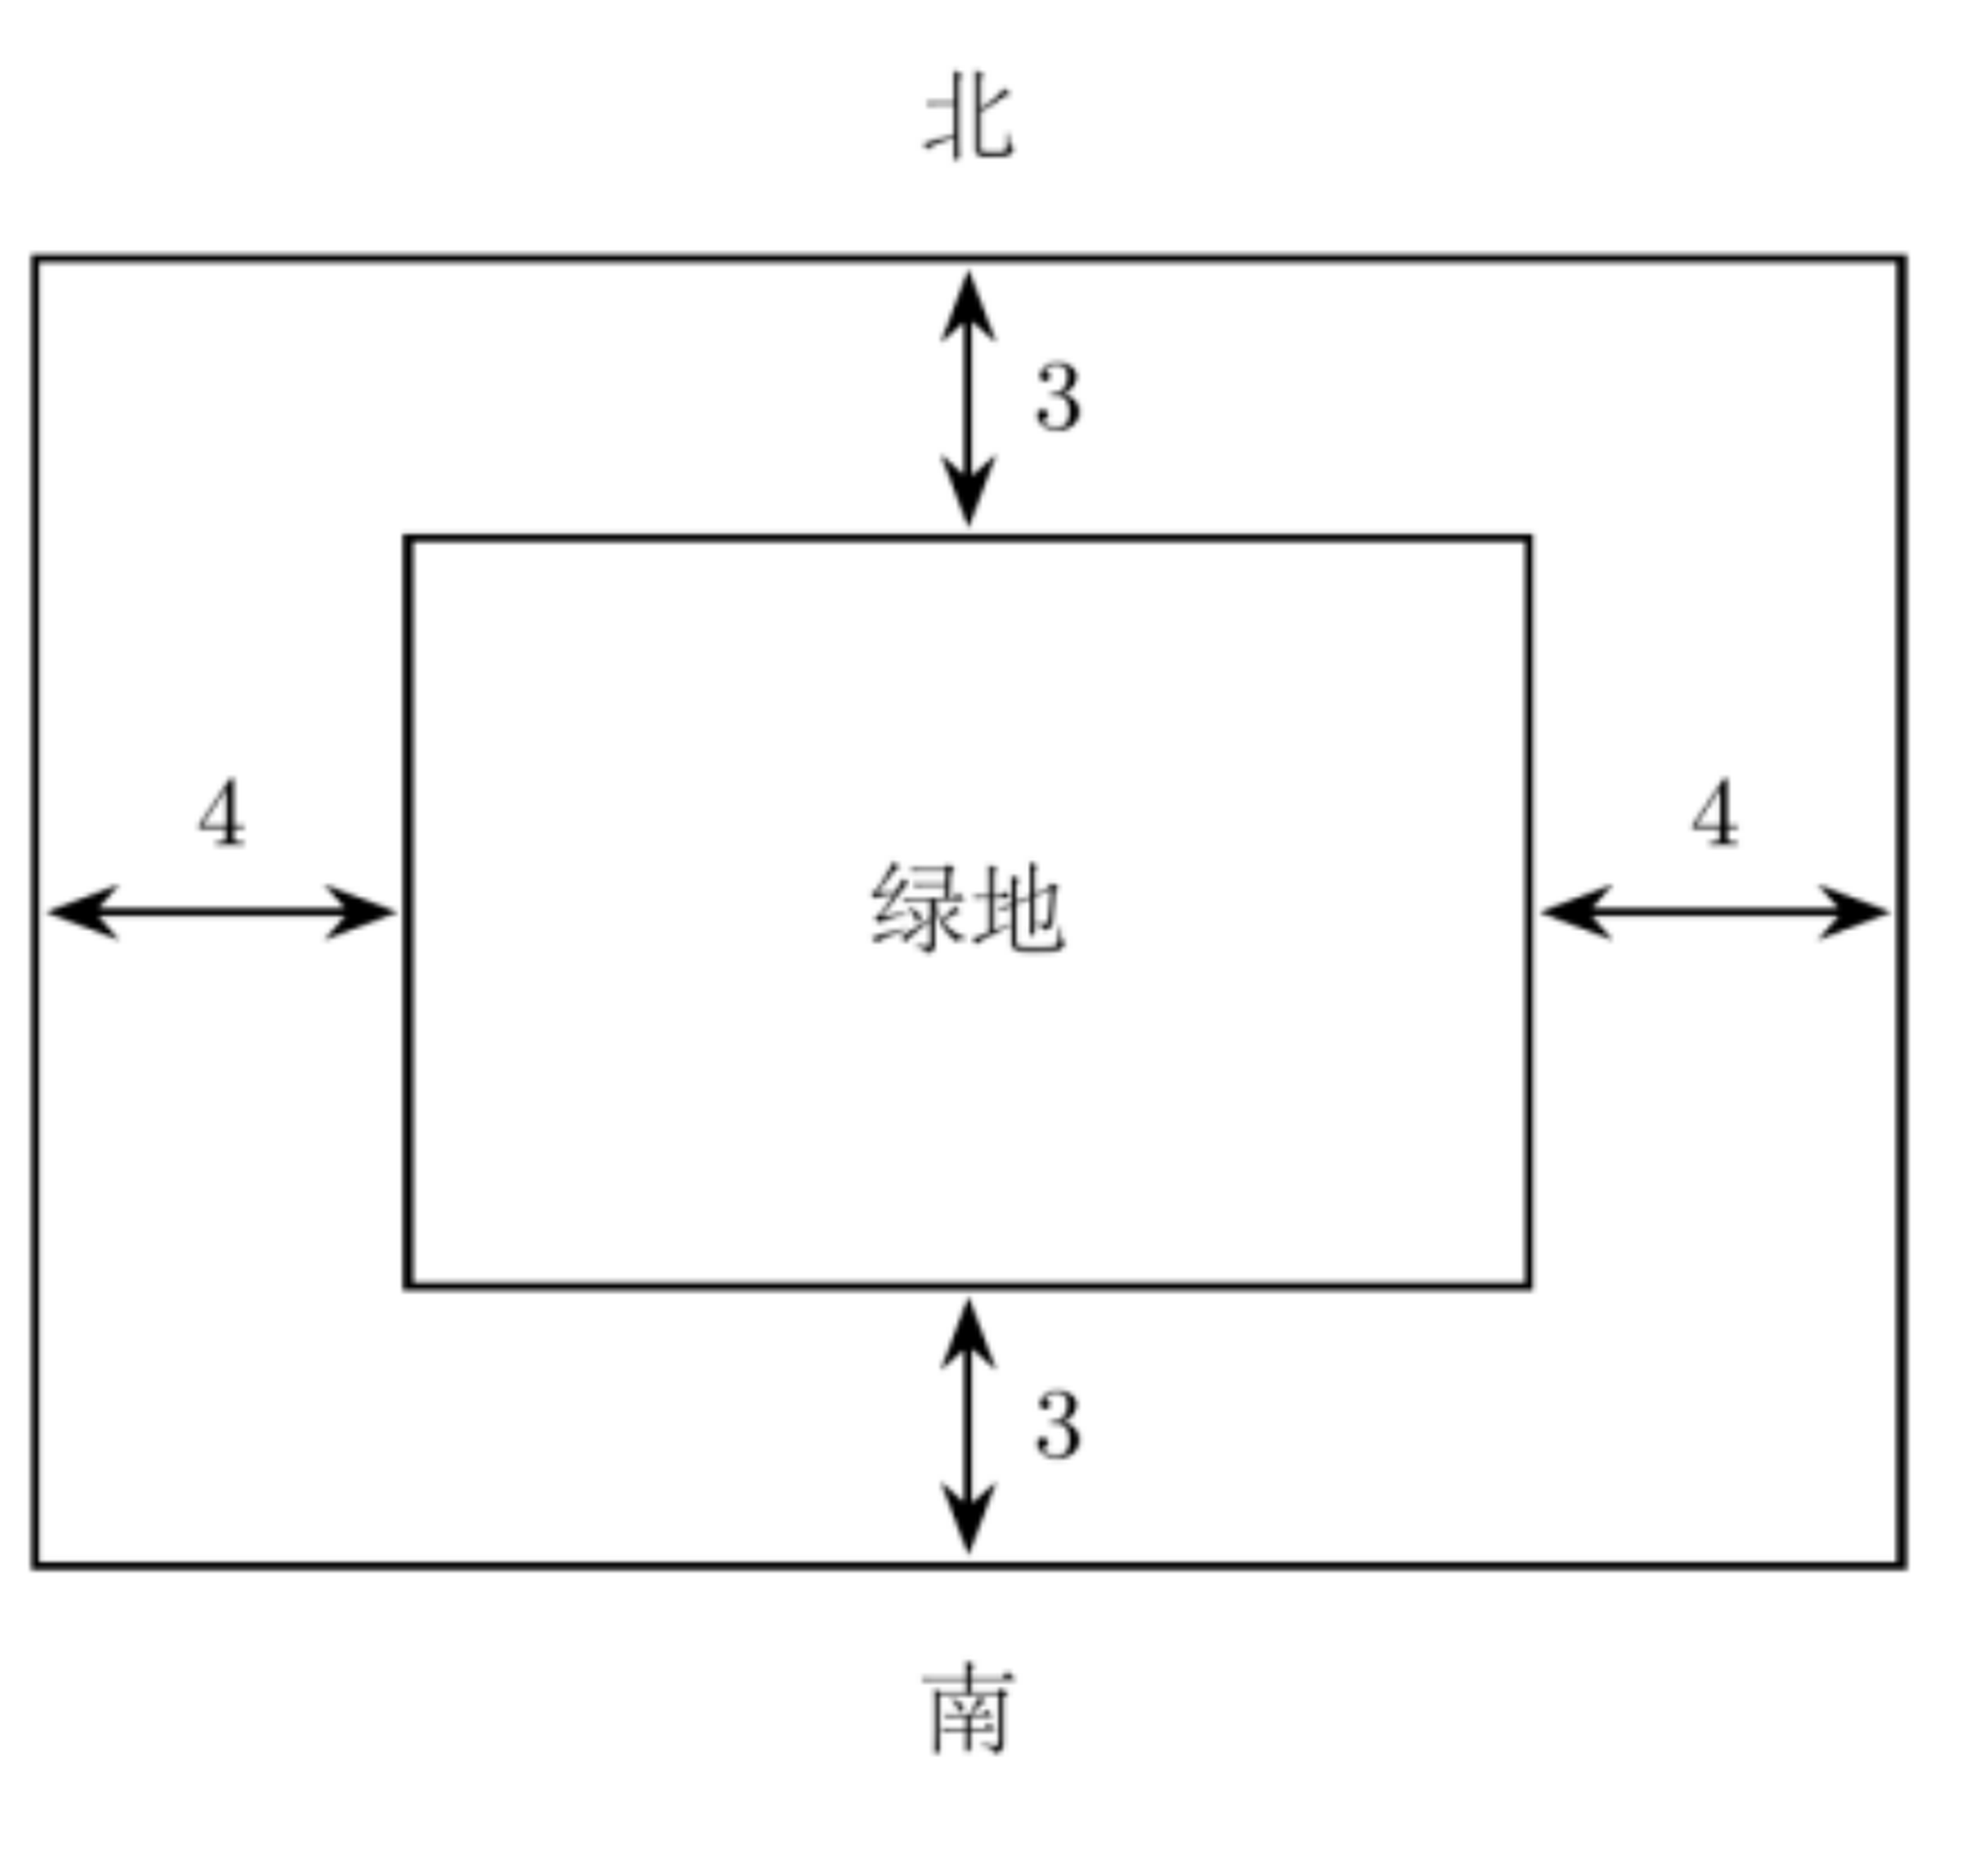
\includegraphics[width=0.32\textwidth]{figures/gao129_q19.png}
\end{center}

(1) 将 $S$ 表示为 $x$ 的函数；

(2) 试确定绿地东西方向的边长和南北方向的边长，使人行道的占地面积最小，并求出人行道的占地最小面积（结果精确到 0.1 米）

\ifanswer
\solbegin
\step{(1) 绿地南北方向的边长为 $\dfrac{1000}{x}$ 米，$x>0$.}
\step{外矩形东西、南北方向的边长分别为 $x+8$ 米、$\dfrac{1000}{x}+6$ 米.}
\step{因此 $S=(x+8)\left(\dfrac{1000}{x}+6\right)-1000=6x+\dfrac{8000}{x}+48, x>0$.}
\step{(2) 因为 $x>0,S=6x+\dfrac{8000}{x}+48\geqslant2\sqrt{6x\cdot\dfrac{8000}{x}}+48=48+80\sqrt{30}$.}
\step{等号当且仅当 $6x=\dfrac{8000}{x}$，即 $x=\dfrac{20\sqrt{30}}{3}\approx36.5$ 时成立，}
\step{此时绿地南北方向的边长为 $\dfrac{1000}{x}=\dfrac{1000}{\dfrac{20\sqrt{30}}{3}}=5\sqrt{30}\approx27.4$（米），}
\step{所以绿地东西方向、南北方向的边长分别约为 36.5 米、27.4 米时，}
\step{人行道的占地面积最小，最小面积为 $S_{min}=48+80\sqrt{30}\approx486.2$ 平方米.}
\solend
\fi

\item 已知集合 $A=\{x\mid x^2-3x+2=0\},B=\{x\mid x^2-ax+a-1=0\}$，

$C=\{x\mid x^2+2(m+1)x+m^2-5=0\}$.

(1) 若 $A=B$，求实数 $a$ 的值；

(2) 若 $B=\{1\}$，求实数 $a$ 的值；

(3) 若 $A\cap C=C$，求实数 $m$ 的取值范围.

\ifanswer
\solbegin
\step{(1) $A=\{1,2\}$，且 $x^2-ax+a-1=(x-1)(x-a+1)$，所以 $B=\{1,a-1\}$，}
\step{因此 $A=B\Leftrightarrow a-1=2\Leftrightarrow a=3$.}
\step{(2) $B=\{1\}$ 表示原方程只有一个不同的实数根，}
\step{得 $a-1=1$，即 $a=2$.}
\step{当 $a=2$ 时，原方程为 $(x-1)^2=0$，符合题意.}
\step{(3) $A\cap C=C\Leftrightarrow C\subseteq\{1,2\}$，}
\step{方程的判别式为 $\Delta=[2(m+1)]^2-4(m^2-5)=8(m+3)$.}
\step{当 $m<-3$ 时，$\Delta<0, C=\varnothing$，满足条件.}
\step{当 $m=-3$ 时，原方程为 $(x-2)^2=0, C=\{2\}$，满足条件.}
\step{当 $m>-3$ 时，方程有两个不同的实数根，必须有 $C=\{1,2\}$，}
\step{由韦达定理，$\begin{cases}-2(m+1)=1+2=3\\m^2-5=1\cdot2=2\end{cases}$，}
\step{第一式得 $m=-\dfrac52$，但此时 $m^2-5=\dfrac54\neq2$，不合题意.}
\step{因此 $m$ 的取值范围为 $(-\infty,-3]$.}
\solend
\fi

\item 设函数 $f(x)=ax^2+(1-a)x+a-2(a\in\R)$.

(1) 若关于 $x$ 的不等式 $f(x)\leqslant0$ 的解集为 $\left[0,\dfrac12\right]$，求实数 $a$ 的值；

(2) 若不等式 $f(x)\geqslant-2$ 对于实数 $a\in[-1,1]$ 时恒成立，求 $x$ 的取值范围；

(3) 解关于 $x$ 的不等式：$f(x)<a-1$.

\ifanswer
\solbegin
\step{(1) 由题意得 $0,\dfrac12$ 是方程 $ax^2+(1-a)x+a-2=0$ 的两个根，}
\step{则 $\begin{cases}0+\dfrac12=-\dfrac{1-a}{a}\\0\times\dfrac12=\dfrac{a-2}{a}\end{cases}\Rightarrow a=2$；}
\step{(2) $ax^2+(1-a)x+a-2\geqslant-2\Rightarrow a(x^2-x+1)+x\geqslant0$ 对 $a\in[-1,1]$ 恒成立，}
\step{则 $\begin{cases}-(x^2-x+1)+x\geqslant0\\(x^2-x+1)+x\geqslant0\end{cases}\Rightarrow\begin{cases}x=1\\x\in\R\end{cases}\Rightarrow x=1$，则 $x$ 的取值范围为 $\{1\}$；}
\step{(3) $f(x)<a-1$ 等价于 $ax^2+(1-a)x-1<0$，}
\step{当 $a=0$ 时，不等式可化为 $x<1$，解集为 $\{x\mid x<1\}$，}
\step{当 $a>0$ 时，不等式可化为 $(ax+1)(x-1)<0$，解集为 $\{x\mid -\dfrac1a<x<1\}$；}
\step{当 $a<0$ 时，不等式化为 $(ax+1)(x-1)<0$，}
\step{①当 $a=-1$ 时，$-\dfrac1a=1$，不等式的解集为 $\{x\mid x\neq1\}$；}
\step{②当 $-1<a<0$ 时，$-\dfrac1a>1$，不等式的解集为 $\{x\mid x<1$ 或 $x>-\dfrac1a\}$；}
\step{③当 $a<-1$ 时，$-\dfrac1a<1$，不等式的解集为 $\{x\mid x<-\dfrac1a$ 或 $x>1\}$；}
\step{综上，当 $a<-1$ 时，解集为 $\{x\mid x<-\dfrac1a$ 或 $x>1\}$；}
\step{当 $a=-1$ 时，解集为 $\{x\mid x\neq1\}$；}
\step{当 $-1<a<0$ 时，解集为 $\{x\mid x<1$ 或 $x>-\dfrac1a\}$；}
\step{当 $a=0$ 时，解集为 $\{x\mid x<1\}$；}
\step{当 $a>0$ 时，解集为 $\{x\mid -\dfrac1a<x<1\}$.}
\solend
\fi

\end{enumerate}

\end{document}
"
% 紧凑版：xelatex "\def\iscompact{1}% 高一129_立达中学_期中.tex
%   —— 高一上数学"2026-2027 年立达中学高一上期中"（试卷版/答案版）
% 试卷版：xelatex 高一129_立达中学_期中.tex
% 答案版：xelatex "\def\isanswer{1}\input{高一129_立达中学_期中.tex}"
% 紧凑版：xelatex "\def\iscompact{1}\input{高一129_立达中学_期中.tex}"
%
% 原始材料：微信公众号"魔都数学加油站"文章，作者破晓，2026-11-12 18:56 发布；
% 连载"27学年高一129"，原文标题"27学年高一129——2026-2027年上海市立达中学高一上期中"；
% 原文链接：https://mp.weixin.qq.com/s/gJhGsOBiWi7gW62u8EWLYA。
% 正文为 8 张 PNG 页（01、02、03、05、06 为 4762x6735，04、07、08 为 2560x3620），
% 题目下印有【解析】或【答案】，为讲评版。题目、解析均据原图转录；
% 卷面粉红色水印"魔都数学加油站"及公众号页脚未录入。全卷仅第 19 题有 1 幅插图。
%
% 卷首标题：原卷印作"2026-2027 年立达中学高一上期中"（公众号标题中的"上海市"
% 卷面标题行没有，本稿照卷面），年份区间按全稿惯例排 en dash；原卷未印副标题，
% 本卷为期中卷、跨集合与常用逻辑用语／不等式／函数三章，按题目内容标为
% "集合与常用逻辑用语、不等式、函数"（与 125、126 同为期中卷，口径相同）：
% 集合与逻辑见 Q3、Q4、Q13、Q20，不等式见 Q5、Q6、Q7、Q9、Q10、Q11、Q12、
% Q14、Q15、Q16、Q17、Q18、Q21，函数（含二次函数、基本不等式应用）见 Q8、Q19、Q21。
%
% 与原卷的排版差异：
%   ① 原文从第 3 题起，填空题编号为 3—12、选择题为 13—16、解答题为 17—21，本稿保留原题号；
%   ② 原卷每题下直接印【解析】／【答案】，本稿按全稿惯例置于答案版；第 3、5 题只印
%      【答案】，另提 \ans{}；第 13—16 题答案均在【解析】末句"故选 …"，题干括号内留空、
%      不另提 \ans{}；四道选择题括号内原卷均未印答案；
%   ③ 原卷未印副标题，本稿按"知识模块"口径补出（见上"卷首标题"）；
%   ④ 原卷填空横线按全稿惯例排为 \blankline[4.4em]；选择题括号排 \mbox{（\quad）}、
%      选项段前按惯例加 \keepwithprev；解答题不留作答区（原卷为讲评版，与 109—128 同）；
%   ⑤ 原卷数集排斜体 $R$，按全稿惯例改 \R；绝对值排 \lvert…\rvert，集合描述竖线排 \mid；
%      不等号按全稿惯例排 \leqslant／\geqslant；子题标号原卷一律用半角括号 (1)(2)(3)，本稿照录；
%   ⑥ 原卷第 19 题插图浮排在 Q18 解析右侧、"19."题干之上，本稿按体例就近置于 Q19
%      题干"如图所示"之后（居中 \includegraphics），图取原卷截图去水印；题前按惯例加
%      \needvspace{7cm} 守卫（照 高一120／127 成例），保证"题干 + 图"整块不被页边界切开；
%   ⑦ 原卷 Q8 解析续头印在第 2 页页首、Q17 解析续头印在第 5 页页首、Q19 题干续在第 6 页、
%      Q20 解析跨 6—7 页、Q21 解析续头印在第 8 页页首，本稿按题合并连续排版；
%      末页第 8 页为 Q21 解析的续尾，按实际印刷行单列（照 高一127 第 09 页续尾成例）。
%
% 判别式字形：第 8 题解析 $\Delta=m^2+4m>0$、第 10 题解析 $\Delta=k^2+6k=k(k+6)<0$、
%   第 20 题 (3) 解析 $\Delta=[2(m+1)]^2-4(m^2-5)=8(m+3)$ 三处原卷均排 $\Delta$
%   （等腰、高；回原图逐处放大核对、三处字形一致），照录 \Delta；全卷未出现 \triangle
%   （等边、扁）。
%
% 子集符号：第 13 题 ② $\{0,1,2\}\subseteq\{2,1,0\}$、③ $\varnothing\subseteq\{0,1,2\}$，
%   第 17 题 (2)② $B\subseteq A$、$B\subseteq(3,+\infty)$，第 20 题 (3) $C\subseteq\{1,2\}$
%   均印带下划线，照录 \subseteq；全卷未出现单线 \subset（回原图放大逐处确认）。
%
% 原卷存疑照录：
%   第 15 题解析"即 $m=4$，$n=3$ 时取等号"与题干 $\dfrac1m+n=1$、等号条件
%     $mn=\dfrac9{mn}$ 均不一致（按题应为 $n=\dfrac34$），照录、未统一；
%   第 18 题 (1) 题干"设 $M=2x^2+3x-1,N=7x-3$ 比较 $M$ 与 $N$ 两个数的大小"
%     两式间用半角逗号、且"$N=7x-3$"后无标点直接接"比较"，照录；
%   第 11 题解析"$1-x+2x-1=-(3x-2), 4x=2, x=\dfrac12$"、第 14 题解析
%     "$a=2, b=1, c=4, d=0$"、第 19 题解析"$6x+\dfrac{8000}{x}+48, x>0$"、
%     第 20 题解析"$\Delta<0, C=\varnothing$"与"$(x-2)^2=0, C=\{2\}$"、
%     第 12 题解析"$(x+y)^2=3+t\geqslant0,(x-y)^2=3-3t\geqslant0$"等处数学式内
%     用半角逗号，照录；
%   第 19 题题干"如图所示（图中单位：米）设绿地东西方向的边长为 $x$"在右括号后
%     无标点直接续"设"，照录；
%   第 21 题 (3) 解析先按 $a>0$、$a=0$、$a<0$ 分述解集，又在"综上"处重列全部
%     五类（含已给出的 $a>0$、$a=0$），照录；
%   第 21 题 (2) 题干与解析均作 $f(x)\geqslant-2$（与 $a(x^2-x+1)+x\geqslant0$ 相符），
%     照录，勿误读为 $f(x)\geqslant2$。
%
% 行数复核：逐题数 \step 条数，合计 93 条（Q3：0；Q4：2；Q5：0；Q6：3；Q7：3；
% Q8：2；Q9：4；Q10：3；Q11：5；Q12：5；Q13：1；Q14：3；Q15：3；Q16：7；
% Q17：7；Q18：8；Q19：8；Q20：13；Q21：16），与原卷印刷行逐题相等
% （cases 块作一个印刷行计）。第 3、5 题只印【答案】，提 \ans{}，不计入 \step 账；
% 四道选择题答案均在解析末句，括号内留空、不另提 \ans{}。
%
\documentclass[a4paper,11pt]{article}
\usepackage{common}

\begin{document}

\examtitlest[3]{2026--2027 年立达中学高一上期中}{集合与常用逻辑用语、不等式、函数}

\bigsec{一、填空题}

\begin{enumerate}
\setcounter{enumi}{2}

\item 若 $A=\{x\mid -3<x\leqslant2\},B=\{x\mid 1<x\leqslant3\}$，则 $A\cup B=$\blankline[4.4em].

\ifanswer
\ans{$(-3,3]$}
\fi

\item 若 $A$ 是 $B$ 的必要非充分条件，$B$ 是 $C$ 的充要条件，$C$ 是 $D$ 的必要非充分条件，则 $D$ 是 $A$ 的\blankline[4.4em]条件.

\ifanswer
\solbegin
\step{$D\Rightarrow C\Leftrightarrow B\Rightarrow A$，且 $A\nRightarrow B$，因此 $D\Rightarrow A$ 且 $A\nRightarrow D$，}
\step{故 $D$ 是 $A$ 的充分非必要条件.}
\solend
\fi

\item 不等式 $\dfrac1x<1$ 的解集为\blankline[4.4em].

\ifanswer
\ans{$(-\infty,0)\cup(1,+\infty)$}
\fi

\item 已知正实数 $x$、$y$ 满足 $2x+y=2$，则 $xy$ 的最大值为\blankline[4.4em].

\ifanswer
\solbegin
\step{因为 $x>0$，$y>0$，所以 $2x+y\geqslant2\sqrt{2xy}$（当且仅当 $2x=y$ 时，取等号），}
\step{又因为 $2x+y=2$，所以 $2\geqslant2\sqrt{2xy}$（当且仅当 $2x=y$ 时，取等号），}
\step{即 $xy\leqslant\dfrac12$，则 $xy$ 的最大值为 $\dfrac12$.}
\solend
\fi

\item 已知 $x\in\R$，函数 $y=\lvert x+2\rvert+\lvert x-3\rvert$ 的最小值为\blankline[4.4em].

\ifanswer
\solbegin
\step{由 $\lvert x+2\rvert+\lvert x-3\rvert\geqslant\lvert(x+2)-(x-3)\rvert=5$，}
\step{当且仅当 $(x+2)(x-3)\leqslant0$，即 $-2\leqslant x\leqslant3$ 时，上式取等号，}
\step{则函数 $y=\lvert x+2\rvert+\lvert x-3\rvert$ 的最小值是 5.}
\solend
\fi

\item 已知实系数一元二次方程 $x^2+mx-m=0$ 的两根分别为 $x_1,x_2$，且 $\lvert x_1-x_2\rvert=\sqrt{21}$，实数 $m$ 的值为\blankline[4.4em].

\ifanswer
\solbegin
\step{由题意得 $\Delta=m^2+4m>0$，解得 $m>0$ 或 $m<-4,x_1+x_2=-m,x_1x_2=-m$，}
\step{则 $\lvert x_1-x_2\rvert=\sqrt{(x_1+x_2)^2-4x_1x_2}=\sqrt{m^2+4m}=\sqrt{21}$，解得 $m=-7$ 或 $3$.}
\solend
\fi

\item 已知不等式 $ax^2-5x+b>0$ 的解集是 $\{x\mid -3<x<-2\}$，则不等式 $bx^2-5x+a>0$ 的解集是\blankline[4.4em].

\ifanswer
\solbegin
\step{$ax^2-5x+b=a(x+3)(x+2)$，比较系数得 $5a=-5,b=6a$，}
\step{即 $a=-1,b=-6$.}
\step{$bx^2-5x+a>0\Leftrightarrow(3x+1)(2x+1)<0\Leftrightarrow-\dfrac12<x<-\dfrac13$，}
\step{故解集为 $\left\{x\mid -\dfrac12<x<-\dfrac13\right\}$.}
\solend
\fi

\item 不等式 $4kx^2+kx-\dfrac38<0$ 对于一切实数 $x$ 都成立，则实数 $k$ 的取值范围是\blankline[4.4em].

\ifanswer
\solbegin
\step{$k=0$ 时，不等式恒成立；}
\step{$k\neq0$ 时，须 $4k<0$ 且 $\Delta=k^2+6k=k(k+6)<0$，解得 $-6<k<0$.}
\step{因此 $k\in(-6,0]$.}
\solend
\fi

\item 设 $x\in\R$，方程 $\lvert 1-x\rvert+\lvert 2x-1\rvert=\lvert 3x-2\rvert$ 的解集为\blankline[4.4em].

\ifanswer
\solbegin
\step{当 $x\leqslant\dfrac12$ 时，方程化为 $1-x-(2x-1)=-(3x-2)$，$2-3x=-3x+2$，恒成立，}
\step{当 $\dfrac12<x\leqslant\dfrac23$ 时，方程化为 $1-x+2x-1=-(3x-2), 4x=2, x=\dfrac12$，不合题意，}
\step{当 $\dfrac23<x\leqslant1$ 时，方程化为 $1-x+2x-1=3x-2$，$2x=2$，解得 $x=1$，}
\step{当 $x>1$ 时，方程化为 $-(1-x)+2x-1=3x-2$，$3x-2=3x-2$，恒成立，}
\step{综上所述，$\lvert 1-x\rvert+\lvert 2x-1\rvert=\lvert 3x-2\rvert$ 的解集为 $\left(-\infty,\dfrac12\right]\cup[1,+\infty)$.}
\solend
\fi

\item 已知非零实数 $x,y$ 满足 $x^2+xy+y^2=3$，则 $x^2-xy+y^2$ 的取值范围是\blankline[4.4em].

\ifanswer
\solbegin
\step{令 $t=xy\neq0$，由 $(x+y)^2=3+t\geqslant0,(x-y)^2=3-3t\geqslant0$，}
\step{得 $t\in[-3,0)\cup(0,1]$.}
\step{对上述任意 $t$，联立 $x+y=\sqrt{3+t},x-y=\sqrt{3-3t}$，所得 $x,y$ 满足原条件，}
\step{因此上述 $t$ 均可取到.}
\step{于是 $x^2-xy+y^2=3-2t$ 的取值范围为 $[1,3)\cup(3,9]$.}
\solend
\fi

\end{enumerate}

\bigsec{二、选择题}

\begin{enumerate}
\setcounter{enumi}{12}

\item 下列各式中，正确的个数是\mbox{（\quad）}

① $\{0\}\in\{0,1,2\}$；② $\{0,1,2\}\subseteq\{2,1,0\}$；③ $\varnothing\subseteq\{0,1,2\}$；④ $\varnothing=\{0\}$；⑤ $\{0,1\}=\{(0,1)\}$；

⑥ $0=\{0\}$.

\keepwithprev
A. $1$\qquad\qquad B. $2$\qquad\qquad C. $3$\qquad\qquad D. $4$

\ifanswer
\solbegin
\step{①不正确，②正确，③正确，④不正确，⑤不正确，⑥不正确. 故选 $B$.}
\solend
\fi

\item 下列四个命题中，为真命题的是\mbox{（\quad）}

\keepwithprev
A. 若 $a>b$，则 $ac^2>bc^2$\qquad\qquad B. 若 $a>b,c>d$，则 $a-c>b-d$

C. 若 $ac^2>bc^2$，则 $a>b$\qquad\qquad D. 若 $a>b$，则 $\dfrac1a<\dfrac1b$

\ifanswer
\solbegin
\step{C 中，$(a-b)c^2>0$，必有 $c^2>0$ 且 $a-b>0$，即 $a>b$.}
\step{A 取 $c=0$；B 取 $a=2, b=1, c=4, d=0$；D 取 $a=1, b=-1$，均不成立.}
\step{故选 $C$.}
\solend
\fi

\item 已知 $m$、$n\in(0,+\infty)$，$\dfrac1m+n=1$，则 $m+\dfrac9n$ 的最小值为\mbox{（\quad）}

\keepwithprev
A. $13$\qquad\qquad B. $16$\qquad\qquad C. $3$\qquad\qquad D. $6$

\ifanswer
\solbegin
\step{因为 $m$、$n\in(0,+\infty)$，$\dfrac1m+n=1$，}
\step{所以 $m+\dfrac9n=(m+\dfrac9n)(\dfrac1m+n)=10+mn+\dfrac9{mn}\geqslant10+2\sqrt{mn\cdot\dfrac9{mn}}=16$，}
\step{当且仅当 $mn=\dfrac9{mn}$，即 $m=4$，$n=3$ 时取等号. 故选 $B$.}
\solend
\fi

\item 下列不等式：① $\left\lvert x+\dfrac1x\right\rvert\geqslant2$；② $x^2+2x+1>0$；③ $\lvert x\rvert+\lvert x-1\rvert\geqslant1$；④ $\dfrac{x}{x^2+x+1}<1$；

解集为 $\R$ 的不等式的个数是\mbox{（\quad）}

\keepwithprev
A. $0$\qquad\qquad B. $1$\qquad\qquad C. $2$\qquad\qquad D. $3$

\ifanswer
\solbegin
\step{对于①，当 $x=0$ 时，$\dfrac1x$ 无意义，故 $\left\lvert x+\dfrac1x\right\rvert\geqslant2$ 的解集不是 $\R$，错误；}
\step{对于②，$x^2+2x+1=(x+1)^2\geqslant0$，当 $x=-1$ 取到等号，解集不是 $\R$，故错误；}
\step{对于③，$\lvert x\rvert+\lvert x-1\rvert\geqslant\lvert x-(x-1)\rvert=1$，当 $x(x-1)\leqslant0$ 时取等号，解集为 $\R$，}
\step{故正确；}
\step{对于④，由于 $x^2+x+1>0$ 恒成立，}
\step{故 $\dfrac{x}{x^2+x+1}<1$ 等价于 $x<x^2+x+1\Rightarrow x^2+1>0$ 恒成立，故解集为 $\R$，正确，}
\step{故正确的有③④，故选 $C$.}
\solend
\fi

\end{enumerate}

\bigsec{三、解答题}

\begin{enumerate}
\setcounter{enumi}{16}

\item (1) 解不等式组 $\begin{cases}\dfrac{x+3}{x+1}\leqslant2\\\lvert 2x-3\rvert\leqslant2\end{cases}$.

(2) 已知集合 $A=\{x\mid -x+3<0\},B=\{x\mid a\leqslant x\leqslant a+3\}$.

①当 $a=2$，求集合 $A\cap B$；

②若 $A\cup B=A$，求实数 $a$ 的取值范围.

\ifanswer
\solbegin
\step{(1) 由 $\begin{cases}\dfrac{x+3}{x+1}\leqslant2\\\lvert 2x-3\rvert\leqslant2\end{cases}$ 得 $\begin{cases}\dfrac{x+3-2x-2}{x+1}\leqslant0\\-2\leqslant2x-3\leqslant2\end{cases}$，即 $\begin{cases}\dfrac{-x+1}{x+1}\leqslant0\\1\leqslant2x\leqslant5\end{cases}$，则 $\begin{cases}\dfrac{x-1}{x+1}\geqslant0\\\dfrac12\leqslant x\leqslant\dfrac52\end{cases}$，}
\step{解得 $1\leqslant x\leqslant\dfrac52$，即原不等式组的解集为 $\left[1,\dfrac52\right]$.}
\step{(2) $-x+3<0\Leftrightarrow x>3$，所以 $A=(3,+\infty)$.}
\step{①当 $a=2$ 时，$B=[2,5], A\cap B=(3,+\infty)\cap[2,5]=(3,5]$.}
\step{②$A\cup B=A\Leftrightarrow B\subseteq A$.}
\step{因为 $B=[a,a+3]$，且左端点 $a\in B$，所以 $B\subseteq(3,+\infty)\Leftrightarrow a>3$，}
\step{实数 $a$ 的取值范围为 $(3,+\infty)$.}
\solend
\fi

\item (1) 设 $M=2x^2+3x-1,N=7x-3$ 比较 $M$ 与 $N$ 两个数的大小.

(2) 解关于 $x$ 的不等式：$x^2-(a+3)x+3a<0$，$a\in\R$.

\ifanswer
\solbegin
\step{(1) $M-N=2x^2+3x-1-(7x-3)=2(x-1)^2$.}
\step{$x=1$ 时，$M-N=0$，即 $M=N$.}
\step{$x\neq1$ 时，$M-N>0$，即 $M>N$.}
\step{(2) 不等式 $x^2-(a+3)x+3a<0$ 可化为 $(x-3)(x-a)<0$，}
\step{不等式对应方程的解为 $a$ 和 3，}
\step{当 $a<3$ 时，不等式 $x^2-(a+3)x+3a<0$ 的解集为 $(a,3)$，}
\step{当 $a=3$ 时，不等式 $x^2-(a+3)x+3a<0$ 的解集为 $\varnothing$，}
\step{当 $a>3$ 时，不等式 $x^2-(a+3)x+3a<0$ 的解集为 $(3,a)$.}
\solend
\fi

% 第 19 题是"题干 + 图"约 7cm 的一整块，答案版实测断点落在题干之后（图被推到次页页首），
% 照 高一120／127 成例在题前先量一次页高，不够就把"题干 + 图"整块一起挪到次页。
\needvspace{7cm}
\item 某新建居民小区欲建一面积为 1000 平方米的矩形绿地，在绿地四周铺设人行道，设计要求绿地南北两侧人行道宽 3 米，东西两侧人行道宽 4 米，如图所示（图中单位：米）设绿地东西方向的边长为 $x$，人行道的占地面积为 $S$.

\begin{center}
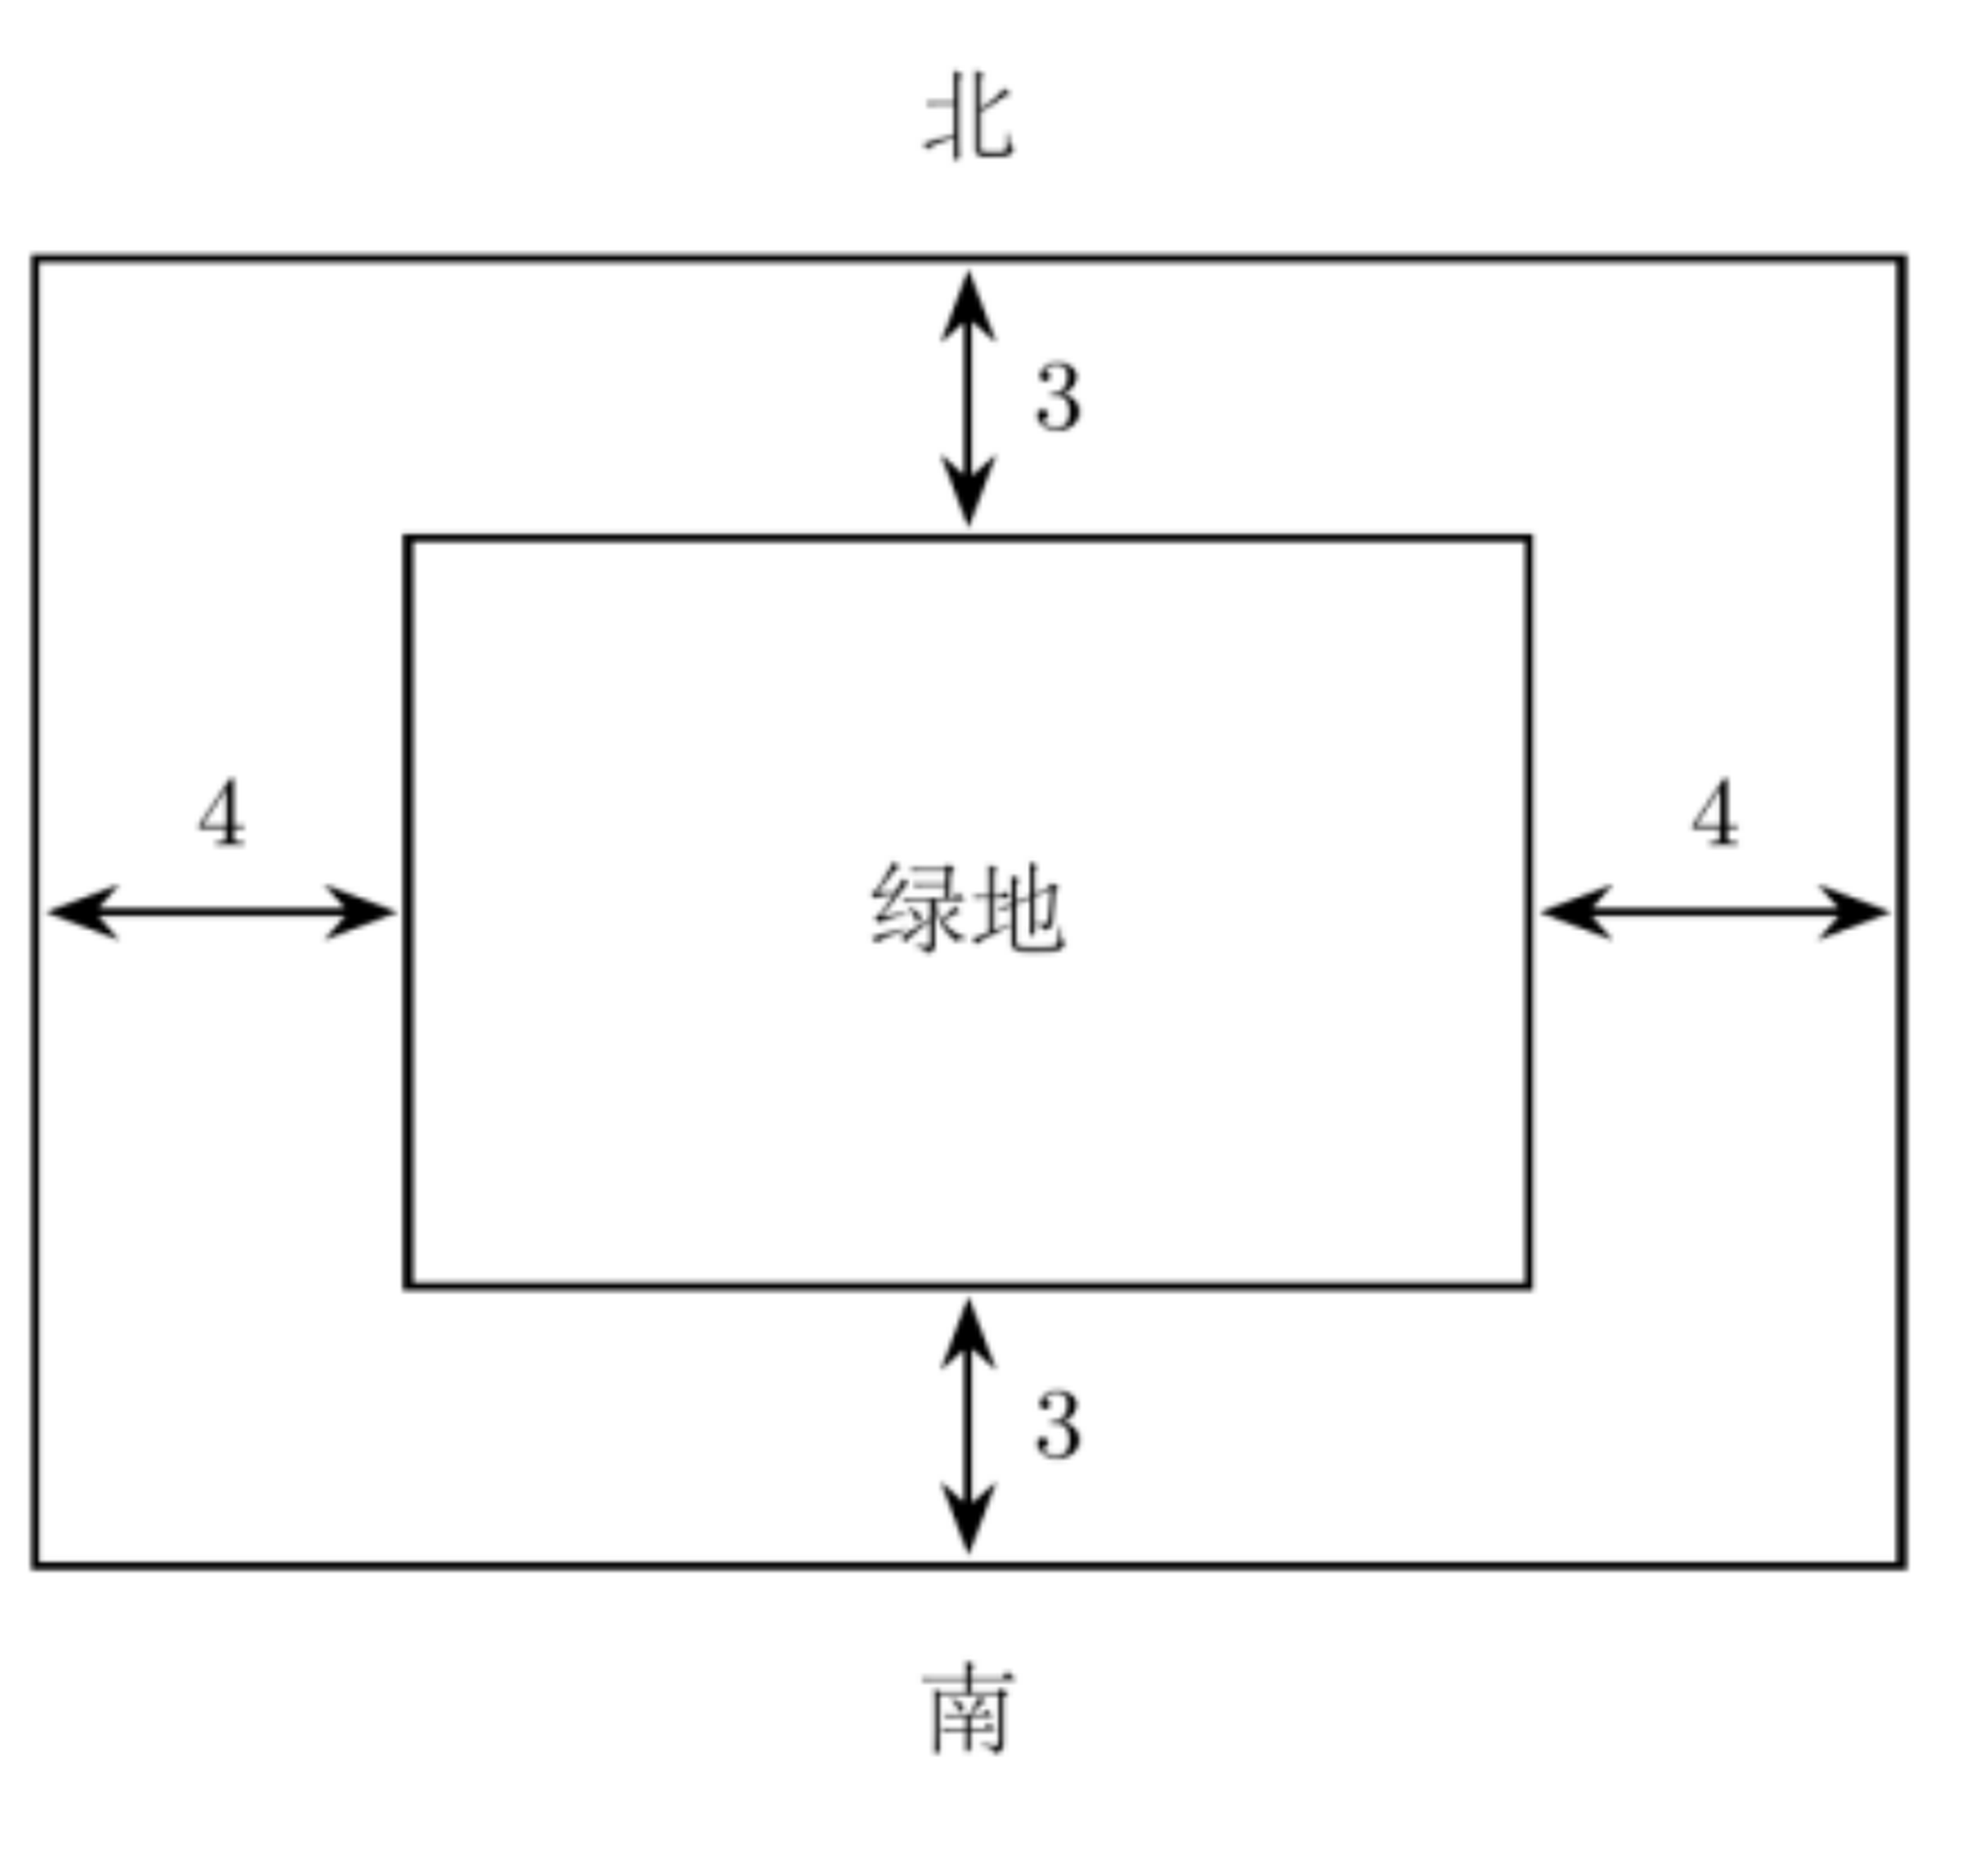
\includegraphics[width=0.32\textwidth]{figures/gao129_q19.png}
\end{center}

(1) 将 $S$ 表示为 $x$ 的函数；

(2) 试确定绿地东西方向的边长和南北方向的边长，使人行道的占地面积最小，并求出人行道的占地最小面积（结果精确到 0.1 米）

\ifanswer
\solbegin
\step{(1) 绿地南北方向的边长为 $\dfrac{1000}{x}$ 米，$x>0$.}
\step{外矩形东西、南北方向的边长分别为 $x+8$ 米、$\dfrac{1000}{x}+6$ 米.}
\step{因此 $S=(x+8)\left(\dfrac{1000}{x}+6\right)-1000=6x+\dfrac{8000}{x}+48, x>0$.}
\step{(2) 因为 $x>0,S=6x+\dfrac{8000}{x}+48\geqslant2\sqrt{6x\cdot\dfrac{8000}{x}}+48=48+80\sqrt{30}$.}
\step{等号当且仅当 $6x=\dfrac{8000}{x}$，即 $x=\dfrac{20\sqrt{30}}{3}\approx36.5$ 时成立，}
\step{此时绿地南北方向的边长为 $\dfrac{1000}{x}=\dfrac{1000}{\dfrac{20\sqrt{30}}{3}}=5\sqrt{30}\approx27.4$（米），}
\step{所以绿地东西方向、南北方向的边长分别约为 36.5 米、27.4 米时，}
\step{人行道的占地面积最小，最小面积为 $S_{min}=48+80\sqrt{30}\approx486.2$ 平方米.}
\solend
\fi

\item 已知集合 $A=\{x\mid x^2-3x+2=0\},B=\{x\mid x^2-ax+a-1=0\}$，

$C=\{x\mid x^2+2(m+1)x+m^2-5=0\}$.

(1) 若 $A=B$，求实数 $a$ 的值；

(2) 若 $B=\{1\}$，求实数 $a$ 的值；

(3) 若 $A\cap C=C$，求实数 $m$ 的取值范围.

\ifanswer
\solbegin
\step{(1) $A=\{1,2\}$，且 $x^2-ax+a-1=(x-1)(x-a+1)$，所以 $B=\{1,a-1\}$，}
\step{因此 $A=B\Leftrightarrow a-1=2\Leftrightarrow a=3$.}
\step{(2) $B=\{1\}$ 表示原方程只有一个不同的实数根，}
\step{得 $a-1=1$，即 $a=2$.}
\step{当 $a=2$ 时，原方程为 $(x-1)^2=0$，符合题意.}
\step{(3) $A\cap C=C\Leftrightarrow C\subseteq\{1,2\}$，}
\step{方程的判别式为 $\Delta=[2(m+1)]^2-4(m^2-5)=8(m+3)$.}
\step{当 $m<-3$ 时，$\Delta<0, C=\varnothing$，满足条件.}
\step{当 $m=-3$ 时，原方程为 $(x-2)^2=0, C=\{2\}$，满足条件.}
\step{当 $m>-3$ 时，方程有两个不同的实数根，必须有 $C=\{1,2\}$，}
\step{由韦达定理，$\begin{cases}-2(m+1)=1+2=3\\m^2-5=1\cdot2=2\end{cases}$，}
\step{第一式得 $m=-\dfrac52$，但此时 $m^2-5=\dfrac54\neq2$，不合题意.}
\step{因此 $m$ 的取值范围为 $(-\infty,-3]$.}
\solend
\fi

\item 设函数 $f(x)=ax^2+(1-a)x+a-2(a\in\R)$.

(1) 若关于 $x$ 的不等式 $f(x)\leqslant0$ 的解集为 $\left[0,\dfrac12\right]$，求实数 $a$ 的值；

(2) 若不等式 $f(x)\geqslant-2$ 对于实数 $a\in[-1,1]$ 时恒成立，求 $x$ 的取值范围；

(3) 解关于 $x$ 的不等式：$f(x)<a-1$.

\ifanswer
\solbegin
\step{(1) 由题意得 $0,\dfrac12$ 是方程 $ax^2+(1-a)x+a-2=0$ 的两个根，}
\step{则 $\begin{cases}0+\dfrac12=-\dfrac{1-a}{a}\\0\times\dfrac12=\dfrac{a-2}{a}\end{cases}\Rightarrow a=2$；}
\step{(2) $ax^2+(1-a)x+a-2\geqslant-2\Rightarrow a(x^2-x+1)+x\geqslant0$ 对 $a\in[-1,1]$ 恒成立，}
\step{则 $\begin{cases}-(x^2-x+1)+x\geqslant0\\(x^2-x+1)+x\geqslant0\end{cases}\Rightarrow\begin{cases}x=1\\x\in\R\end{cases}\Rightarrow x=1$，则 $x$ 的取值范围为 $\{1\}$；}
\step{(3) $f(x)<a-1$ 等价于 $ax^2+(1-a)x-1<0$，}
\step{当 $a=0$ 时，不等式可化为 $x<1$，解集为 $\{x\mid x<1\}$，}
\step{当 $a>0$ 时，不等式可化为 $(ax+1)(x-1)<0$，解集为 $\{x\mid -\dfrac1a<x<1\}$；}
\step{当 $a<0$ 时，不等式化为 $(ax+1)(x-1)<0$，}
\step{①当 $a=-1$ 时，$-\dfrac1a=1$，不等式的解集为 $\{x\mid x\neq1\}$；}
\step{②当 $-1<a<0$ 时，$-\dfrac1a>1$，不等式的解集为 $\{x\mid x<1$ 或 $x>-\dfrac1a\}$；}
\step{③当 $a<-1$ 时，$-\dfrac1a<1$，不等式的解集为 $\{x\mid x<-\dfrac1a$ 或 $x>1\}$；}
\step{综上，当 $a<-1$ 时，解集为 $\{x\mid x<-\dfrac1a$ 或 $x>1\}$；}
\step{当 $a=-1$ 时，解集为 $\{x\mid x\neq1\}$；}
\step{当 $-1<a<0$ 时，解集为 $\{x\mid x<1$ 或 $x>-\dfrac1a\}$；}
\step{当 $a=0$ 时，解集为 $\{x\mid x<1\}$；}
\step{当 $a>0$ 时，解集为 $\{x\mid -\dfrac1a<x<1\}$.}
\solend
\fi

\end{enumerate}

\end{document}
"
%
% 原始材料：微信公众号"魔都数学加油站"文章，作者破晓，2026-11-12 18:56 发布；
% 连载"27学年高一129"，原文标题"27学年高一129——2026-2027年上海市立达中学高一上期中"；
% 原文链接：https://mp.weixin.qq.com/s/gJhGsOBiWi7gW62u8EWLYA。
% 正文为 8 张 PNG 页（01、02、03、05、06 为 4762x6735，04、07、08 为 2560x3620），
% 题目下印有【解析】或【答案】，为讲评版。题目、解析均据原图转录；
% 卷面粉红色水印"魔都数学加油站"及公众号页脚未录入。全卷仅第 19 题有 1 幅插图。
%
% 卷首标题：原卷印作"2026-2027 年立达中学高一上期中"（公众号标题中的"上海市"
% 卷面标题行没有，本稿照卷面），年份区间按全稿惯例排 en dash；原卷未印副标题，
% 本卷为期中卷、跨集合与常用逻辑用语／不等式／函数三章，按题目内容标为
% "集合与常用逻辑用语、不等式、函数"（与 125、126 同为期中卷，口径相同）：
% 集合与逻辑见 Q3、Q4、Q13、Q20，不等式见 Q5、Q6、Q7、Q9、Q10、Q11、Q12、
% Q14、Q15、Q16、Q17、Q18、Q21，函数（含二次函数、基本不等式应用）见 Q8、Q19、Q21。
%
% 与原卷的排版差异：
%   ① 原文从第 3 题起，填空题编号为 3—12、选择题为 13—16、解答题为 17—21，本稿保留原题号；
%   ② 原卷每题下直接印【解析】／【答案】，本稿按全稿惯例置于答案版；第 3、5 题只印
%      【答案】，另提 \ans{}；第 13—16 题答案均在【解析】末句"故选 …"，题干括号内留空、
%      不另提 \ans{}；四道选择题括号内原卷均未印答案；
%   ③ 原卷未印副标题，本稿按"知识模块"口径补出（见上"卷首标题"）；
%   ④ 原卷填空横线按全稿惯例排为 \blankline[4.4em]；选择题括号排 \mbox{（\quad）}、
%      选项段前按惯例加 \keepwithprev；解答题不留作答区（原卷为讲评版，与 109—128 同）；
%   ⑤ 原卷数集排斜体 $R$，按全稿惯例改 \R；绝对值排 \lvert…\rvert，集合描述竖线排 \mid；
%      不等号按全稿惯例排 \leqslant／\geqslant；子题标号原卷一律用半角括号 (1)(2)(3)，本稿照录；
%   ⑥ 原卷第 19 题插图浮排在 Q18 解析右侧、"19."题干之上，本稿按体例就近置于 Q19
%      题干"如图所示"之后（居中 \includegraphics），图取原卷截图去水印；题前按惯例加
%      \needvspace{7cm} 守卫（照 高一120／127 成例），保证"题干 + 图"整块不被页边界切开；
%   ⑦ 原卷 Q8 解析续头印在第 2 页页首、Q17 解析续头印在第 5 页页首、Q19 题干续在第 6 页、
%      Q20 解析跨 6—7 页、Q21 解析续头印在第 8 页页首，本稿按题合并连续排版；
%      末页第 8 页为 Q21 解析的续尾，按实际印刷行单列（照 高一127 第 09 页续尾成例）。
%
% 判别式字形：第 8 题解析 $\Delta=m^2+4m>0$、第 10 题解析 $\Delta=k^2+6k=k(k+6)<0$、
%   第 20 题 (3) 解析 $\Delta=[2(m+1)]^2-4(m^2-5)=8(m+3)$ 三处原卷均排 $\Delta$
%   （等腰、高；回原图逐处放大核对、三处字形一致），照录 \Delta；全卷未出现 \triangle
%   （等边、扁）。
%
% 子集符号：第 13 题 ② $\{0,1,2\}\subseteq\{2,1,0\}$、③ $\varnothing\subseteq\{0,1,2\}$，
%   第 17 题 (2)② $B\subseteq A$、$B\subseteq(3,+\infty)$，第 20 题 (3) $C\subseteq\{1,2\}$
%   均印带下划线，照录 \subseteq；全卷未出现单线 \subset（回原图放大逐处确认）。
%
% 原卷存疑照录：
%   第 15 题解析"即 $m=4$，$n=3$ 时取等号"与题干 $\dfrac1m+n=1$、等号条件
%     $mn=\dfrac9{mn}$ 均不一致（按题应为 $n=\dfrac34$），照录、未统一；
%   第 18 题 (1) 题干"设 $M=2x^2+3x-1,N=7x-3$ 比较 $M$ 与 $N$ 两个数的大小"
%     两式间用半角逗号、且"$N=7x-3$"后无标点直接接"比较"，照录；
%   第 11 题解析"$1-x+2x-1=-(3x-2), 4x=2, x=\dfrac12$"、第 14 题解析
%     "$a=2, b=1, c=4, d=0$"、第 19 题解析"$6x+\dfrac{8000}{x}+48, x>0$"、
%     第 20 题解析"$\Delta<0, C=\varnothing$"与"$(x-2)^2=0, C=\{2\}$"、
%     第 12 题解析"$(x+y)^2=3+t\geqslant0,(x-y)^2=3-3t\geqslant0$"等处数学式内
%     用半角逗号，照录；
%   第 19 题题干"如图所示（图中单位：米）设绿地东西方向的边长为 $x$"在右括号后
%     无标点直接续"设"，照录；
%   第 21 题 (3) 解析先按 $a>0$、$a=0$、$a<0$ 分述解集，又在"综上"处重列全部
%     五类（含已给出的 $a>0$、$a=0$），照录；
%   第 21 题 (2) 题干与解析均作 $f(x)\geqslant-2$（与 $a(x^2-x+1)+x\geqslant0$ 相符），
%     照录，勿误读为 $f(x)\geqslant2$。
%
% 行数复核：逐题数 \step 条数，合计 93 条（Q3：0；Q4：2；Q5：0；Q6：3；Q7：3；
% Q8：2；Q9：4；Q10：3；Q11：5；Q12：5；Q13：1；Q14：3；Q15：3；Q16：7；
% Q17：7；Q18：8；Q19：8；Q20：13；Q21：16），与原卷印刷行逐题相等
% （cases 块作一个印刷行计）。第 3、5 题只印【答案】，提 \ans{}，不计入 \step 账；
% 四道选择题答案均在解析末句，括号内留空、不另提 \ans{}。
%
\documentclass[a4paper,11pt]{article}
\usepackage{common}

\begin{document}

\examtitlest[3]{2026--2027 年立达中学高一上期中}{集合与常用逻辑用语、不等式、函数}

\bigsec{一、填空题}

\begin{enumerate}
\setcounter{enumi}{2}

\item 若 $A=\{x\mid -3<x\leqslant2\},B=\{x\mid 1<x\leqslant3\}$，则 $A\cup B=$\blankline[4.4em].

\ifanswer
\ans{$(-3,3]$}
\fi

\item 若 $A$ 是 $B$ 的必要非充分条件，$B$ 是 $C$ 的充要条件，$C$ 是 $D$ 的必要非充分条件，则 $D$ 是 $A$ 的\blankline[4.4em]条件.

\ifanswer
\solbegin
\step{$D\Rightarrow C\Leftrightarrow B\Rightarrow A$，且 $A\nRightarrow B$，因此 $D\Rightarrow A$ 且 $A\nRightarrow D$，}
\step{故 $D$ 是 $A$ 的充分非必要条件.}
\solend
\fi

\item 不等式 $\dfrac1x<1$ 的解集为\blankline[4.4em].

\ifanswer
\ans{$(-\infty,0)\cup(1,+\infty)$}
\fi

\item 已知正实数 $x$、$y$ 满足 $2x+y=2$，则 $xy$ 的最大值为\blankline[4.4em].

\ifanswer
\solbegin
\step{因为 $x>0$，$y>0$，所以 $2x+y\geqslant2\sqrt{2xy}$（当且仅当 $2x=y$ 时，取等号），}
\step{又因为 $2x+y=2$，所以 $2\geqslant2\sqrt{2xy}$（当且仅当 $2x=y$ 时，取等号），}
\step{即 $xy\leqslant\dfrac12$，则 $xy$ 的最大值为 $\dfrac12$.}
\solend
\fi

\item 已知 $x\in\R$，函数 $y=\lvert x+2\rvert+\lvert x-3\rvert$ 的最小值为\blankline[4.4em].

\ifanswer
\solbegin
\step{由 $\lvert x+2\rvert+\lvert x-3\rvert\geqslant\lvert(x+2)-(x-3)\rvert=5$，}
\step{当且仅当 $(x+2)(x-3)\leqslant0$，即 $-2\leqslant x\leqslant3$ 时，上式取等号，}
\step{则函数 $y=\lvert x+2\rvert+\lvert x-3\rvert$ 的最小值是 5.}
\solend
\fi

\item 已知实系数一元二次方程 $x^2+mx-m=0$ 的两根分别为 $x_1,x_2$，且 $\lvert x_1-x_2\rvert=\sqrt{21}$，实数 $m$ 的值为\blankline[4.4em].

\ifanswer
\solbegin
\step{由题意得 $\Delta=m^2+4m>0$，解得 $m>0$ 或 $m<-4,x_1+x_2=-m,x_1x_2=-m$，}
\step{则 $\lvert x_1-x_2\rvert=\sqrt{(x_1+x_2)^2-4x_1x_2}=\sqrt{m^2+4m}=\sqrt{21}$，解得 $m=-7$ 或 $3$.}
\solend
\fi

\item 已知不等式 $ax^2-5x+b>0$ 的解集是 $\{x\mid -3<x<-2\}$，则不等式 $bx^2-5x+a>0$ 的解集是\blankline[4.4em].

\ifanswer
\solbegin
\step{$ax^2-5x+b=a(x+3)(x+2)$，比较系数得 $5a=-5,b=6a$，}
\step{即 $a=-1,b=-6$.}
\step{$bx^2-5x+a>0\Leftrightarrow(3x+1)(2x+1)<0\Leftrightarrow-\dfrac12<x<-\dfrac13$，}
\step{故解集为 $\left\{x\mid -\dfrac12<x<-\dfrac13\right\}$.}
\solend
\fi

\item 不等式 $4kx^2+kx-\dfrac38<0$ 对于一切实数 $x$ 都成立，则实数 $k$ 的取值范围是\blankline[4.4em].

\ifanswer
\solbegin
\step{$k=0$ 时，不等式恒成立；}
\step{$k\neq0$ 时，须 $4k<0$ 且 $\Delta=k^2+6k=k(k+6)<0$，解得 $-6<k<0$.}
\step{因此 $k\in(-6,0]$.}
\solend
\fi

\item 设 $x\in\R$，方程 $\lvert 1-x\rvert+\lvert 2x-1\rvert=\lvert 3x-2\rvert$ 的解集为\blankline[4.4em].

\ifanswer
\solbegin
\step{当 $x\leqslant\dfrac12$ 时，方程化为 $1-x-(2x-1)=-(3x-2)$，$2-3x=-3x+2$，恒成立，}
\step{当 $\dfrac12<x\leqslant\dfrac23$ 时，方程化为 $1-x+2x-1=-(3x-2), 4x=2, x=\dfrac12$，不合题意，}
\step{当 $\dfrac23<x\leqslant1$ 时，方程化为 $1-x+2x-1=3x-2$，$2x=2$，解得 $x=1$，}
\step{当 $x>1$ 时，方程化为 $-(1-x)+2x-1=3x-2$，$3x-2=3x-2$，恒成立，}
\step{综上所述，$\lvert 1-x\rvert+\lvert 2x-1\rvert=\lvert 3x-2\rvert$ 的解集为 $\left(-\infty,\dfrac12\right]\cup[1,+\infty)$.}
\solend
\fi

\item 已知非零实数 $x,y$ 满足 $x^2+xy+y^2=3$，则 $x^2-xy+y^2$ 的取值范围是\blankline[4.4em].

\ifanswer
\solbegin
\step{令 $t=xy\neq0$，由 $(x+y)^2=3+t\geqslant0,(x-y)^2=3-3t\geqslant0$，}
\step{得 $t\in[-3,0)\cup(0,1]$.}
\step{对上述任意 $t$，联立 $x+y=\sqrt{3+t},x-y=\sqrt{3-3t}$，所得 $x,y$ 满足原条件，}
\step{因此上述 $t$ 均可取到.}
\step{于是 $x^2-xy+y^2=3-2t$ 的取值范围为 $[1,3)\cup(3,9]$.}
\solend
\fi

\end{enumerate}

\bigsec{二、选择题}

\begin{enumerate}
\setcounter{enumi}{12}

\item 下列各式中，正确的个数是\mbox{（\quad）}

① $\{0\}\in\{0,1,2\}$；② $\{0,1,2\}\subseteq\{2,1,0\}$；③ $\varnothing\subseteq\{0,1,2\}$；④ $\varnothing=\{0\}$；⑤ $\{0,1\}=\{(0,1)\}$；

⑥ $0=\{0\}$.

\keepwithprev
A. $1$\qquad\qquad B. $2$\qquad\qquad C. $3$\qquad\qquad D. $4$

\ifanswer
\solbegin
\step{①不正确，②正确，③正确，④不正确，⑤不正确，⑥不正确. 故选 $B$.}
\solend
\fi

\item 下列四个命题中，为真命题的是\mbox{（\quad）}

\keepwithprev
A. 若 $a>b$，则 $ac^2>bc^2$\qquad\qquad B. 若 $a>b,c>d$，则 $a-c>b-d$

C. 若 $ac^2>bc^2$，则 $a>b$\qquad\qquad D. 若 $a>b$，则 $\dfrac1a<\dfrac1b$

\ifanswer
\solbegin
\step{C 中，$(a-b)c^2>0$，必有 $c^2>0$ 且 $a-b>0$，即 $a>b$.}
\step{A 取 $c=0$；B 取 $a=2, b=1, c=4, d=0$；D 取 $a=1, b=-1$，均不成立.}
\step{故选 $C$.}
\solend
\fi

\item 已知 $m$、$n\in(0,+\infty)$，$\dfrac1m+n=1$，则 $m+\dfrac9n$ 的最小值为\mbox{（\quad）}

\keepwithprev
A. $13$\qquad\qquad B. $16$\qquad\qquad C. $3$\qquad\qquad D. $6$

\ifanswer
\solbegin
\step{因为 $m$、$n\in(0,+\infty)$，$\dfrac1m+n=1$，}
\step{所以 $m+\dfrac9n=(m+\dfrac9n)(\dfrac1m+n)=10+mn+\dfrac9{mn}\geqslant10+2\sqrt{mn\cdot\dfrac9{mn}}=16$，}
\step{当且仅当 $mn=\dfrac9{mn}$，即 $m=4$，$n=3$ 时取等号. 故选 $B$.}
\solend
\fi

\item 下列不等式：① $\left\lvert x+\dfrac1x\right\rvert\geqslant2$；② $x^2+2x+1>0$；③ $\lvert x\rvert+\lvert x-1\rvert\geqslant1$；④ $\dfrac{x}{x^2+x+1}<1$；

解集为 $\R$ 的不等式的个数是\mbox{（\quad）}

\keepwithprev
A. $0$\qquad\qquad B. $1$\qquad\qquad C. $2$\qquad\qquad D. $3$

\ifanswer
\solbegin
\step{对于①，当 $x=0$ 时，$\dfrac1x$ 无意义，故 $\left\lvert x+\dfrac1x\right\rvert\geqslant2$ 的解集不是 $\R$，错误；}
\step{对于②，$x^2+2x+1=(x+1)^2\geqslant0$，当 $x=-1$ 取到等号，解集不是 $\R$，故错误；}
\step{对于③，$\lvert x\rvert+\lvert x-1\rvert\geqslant\lvert x-(x-1)\rvert=1$，当 $x(x-1)\leqslant0$ 时取等号，解集为 $\R$，}
\step{故正确；}
\step{对于④，由于 $x^2+x+1>0$ 恒成立，}
\step{故 $\dfrac{x}{x^2+x+1}<1$ 等价于 $x<x^2+x+1\Rightarrow x^2+1>0$ 恒成立，故解集为 $\R$，正确，}
\step{故正确的有③④，故选 $C$.}
\solend
\fi

\end{enumerate}

\bigsec{三、解答题}

\begin{enumerate}
\setcounter{enumi}{16}

\item (1) 解不等式组 $\begin{cases}\dfrac{x+3}{x+1}\leqslant2\\\lvert 2x-3\rvert\leqslant2\end{cases}$.

(2) 已知集合 $A=\{x\mid -x+3<0\},B=\{x\mid a\leqslant x\leqslant a+3\}$.

①当 $a=2$，求集合 $A\cap B$；

②若 $A\cup B=A$，求实数 $a$ 的取值范围.

\ifanswer
\solbegin
\step{(1) 由 $\begin{cases}\dfrac{x+3}{x+1}\leqslant2\\\lvert 2x-3\rvert\leqslant2\end{cases}$ 得 $\begin{cases}\dfrac{x+3-2x-2}{x+1}\leqslant0\\-2\leqslant2x-3\leqslant2\end{cases}$，即 $\begin{cases}\dfrac{-x+1}{x+1}\leqslant0\\1\leqslant2x\leqslant5\end{cases}$，则 $\begin{cases}\dfrac{x-1}{x+1}\geqslant0\\\dfrac12\leqslant x\leqslant\dfrac52\end{cases}$，}
\step{解得 $1\leqslant x\leqslant\dfrac52$，即原不等式组的解集为 $\left[1,\dfrac52\right]$.}
\step{(2) $-x+3<0\Leftrightarrow x>3$，所以 $A=(3,+\infty)$.}
\step{①当 $a=2$ 时，$B=[2,5], A\cap B=(3,+\infty)\cap[2,5]=(3,5]$.}
\step{②$A\cup B=A\Leftrightarrow B\subseteq A$.}
\step{因为 $B=[a,a+3]$，且左端点 $a\in B$，所以 $B\subseteq(3,+\infty)\Leftrightarrow a>3$，}
\step{实数 $a$ 的取值范围为 $(3,+\infty)$.}
\solend
\fi

\item (1) 设 $M=2x^2+3x-1,N=7x-3$ 比较 $M$ 与 $N$ 两个数的大小.

(2) 解关于 $x$ 的不等式：$x^2-(a+3)x+3a<0$，$a\in\R$.

\ifanswer
\solbegin
\step{(1) $M-N=2x^2+3x-1-(7x-3)=2(x-1)^2$.}
\step{$x=1$ 时，$M-N=0$，即 $M=N$.}
\step{$x\neq1$ 时，$M-N>0$，即 $M>N$.}
\step{(2) 不等式 $x^2-(a+3)x+3a<0$ 可化为 $(x-3)(x-a)<0$，}
\step{不等式对应方程的解为 $a$ 和 3，}
\step{当 $a<3$ 时，不等式 $x^2-(a+3)x+3a<0$ 的解集为 $(a,3)$，}
\step{当 $a=3$ 时，不等式 $x^2-(a+3)x+3a<0$ 的解集为 $\varnothing$，}
\step{当 $a>3$ 时，不等式 $x^2-(a+3)x+3a<0$ 的解集为 $(3,a)$.}
\solend
\fi

% 第 19 题是"题干 + 图"约 7cm 的一整块，答案版实测断点落在题干之后（图被推到次页页首），
% 照 高一120／127 成例在题前先量一次页高，不够就把"题干 + 图"整块一起挪到次页。
\needvspace{7cm}
\item 某新建居民小区欲建一面积为 1000 平方米的矩形绿地，在绿地四周铺设人行道，设计要求绿地南北两侧人行道宽 3 米，东西两侧人行道宽 4 米，如图所示（图中单位：米）设绿地东西方向的边长为 $x$，人行道的占地面积为 $S$.

\begin{center}
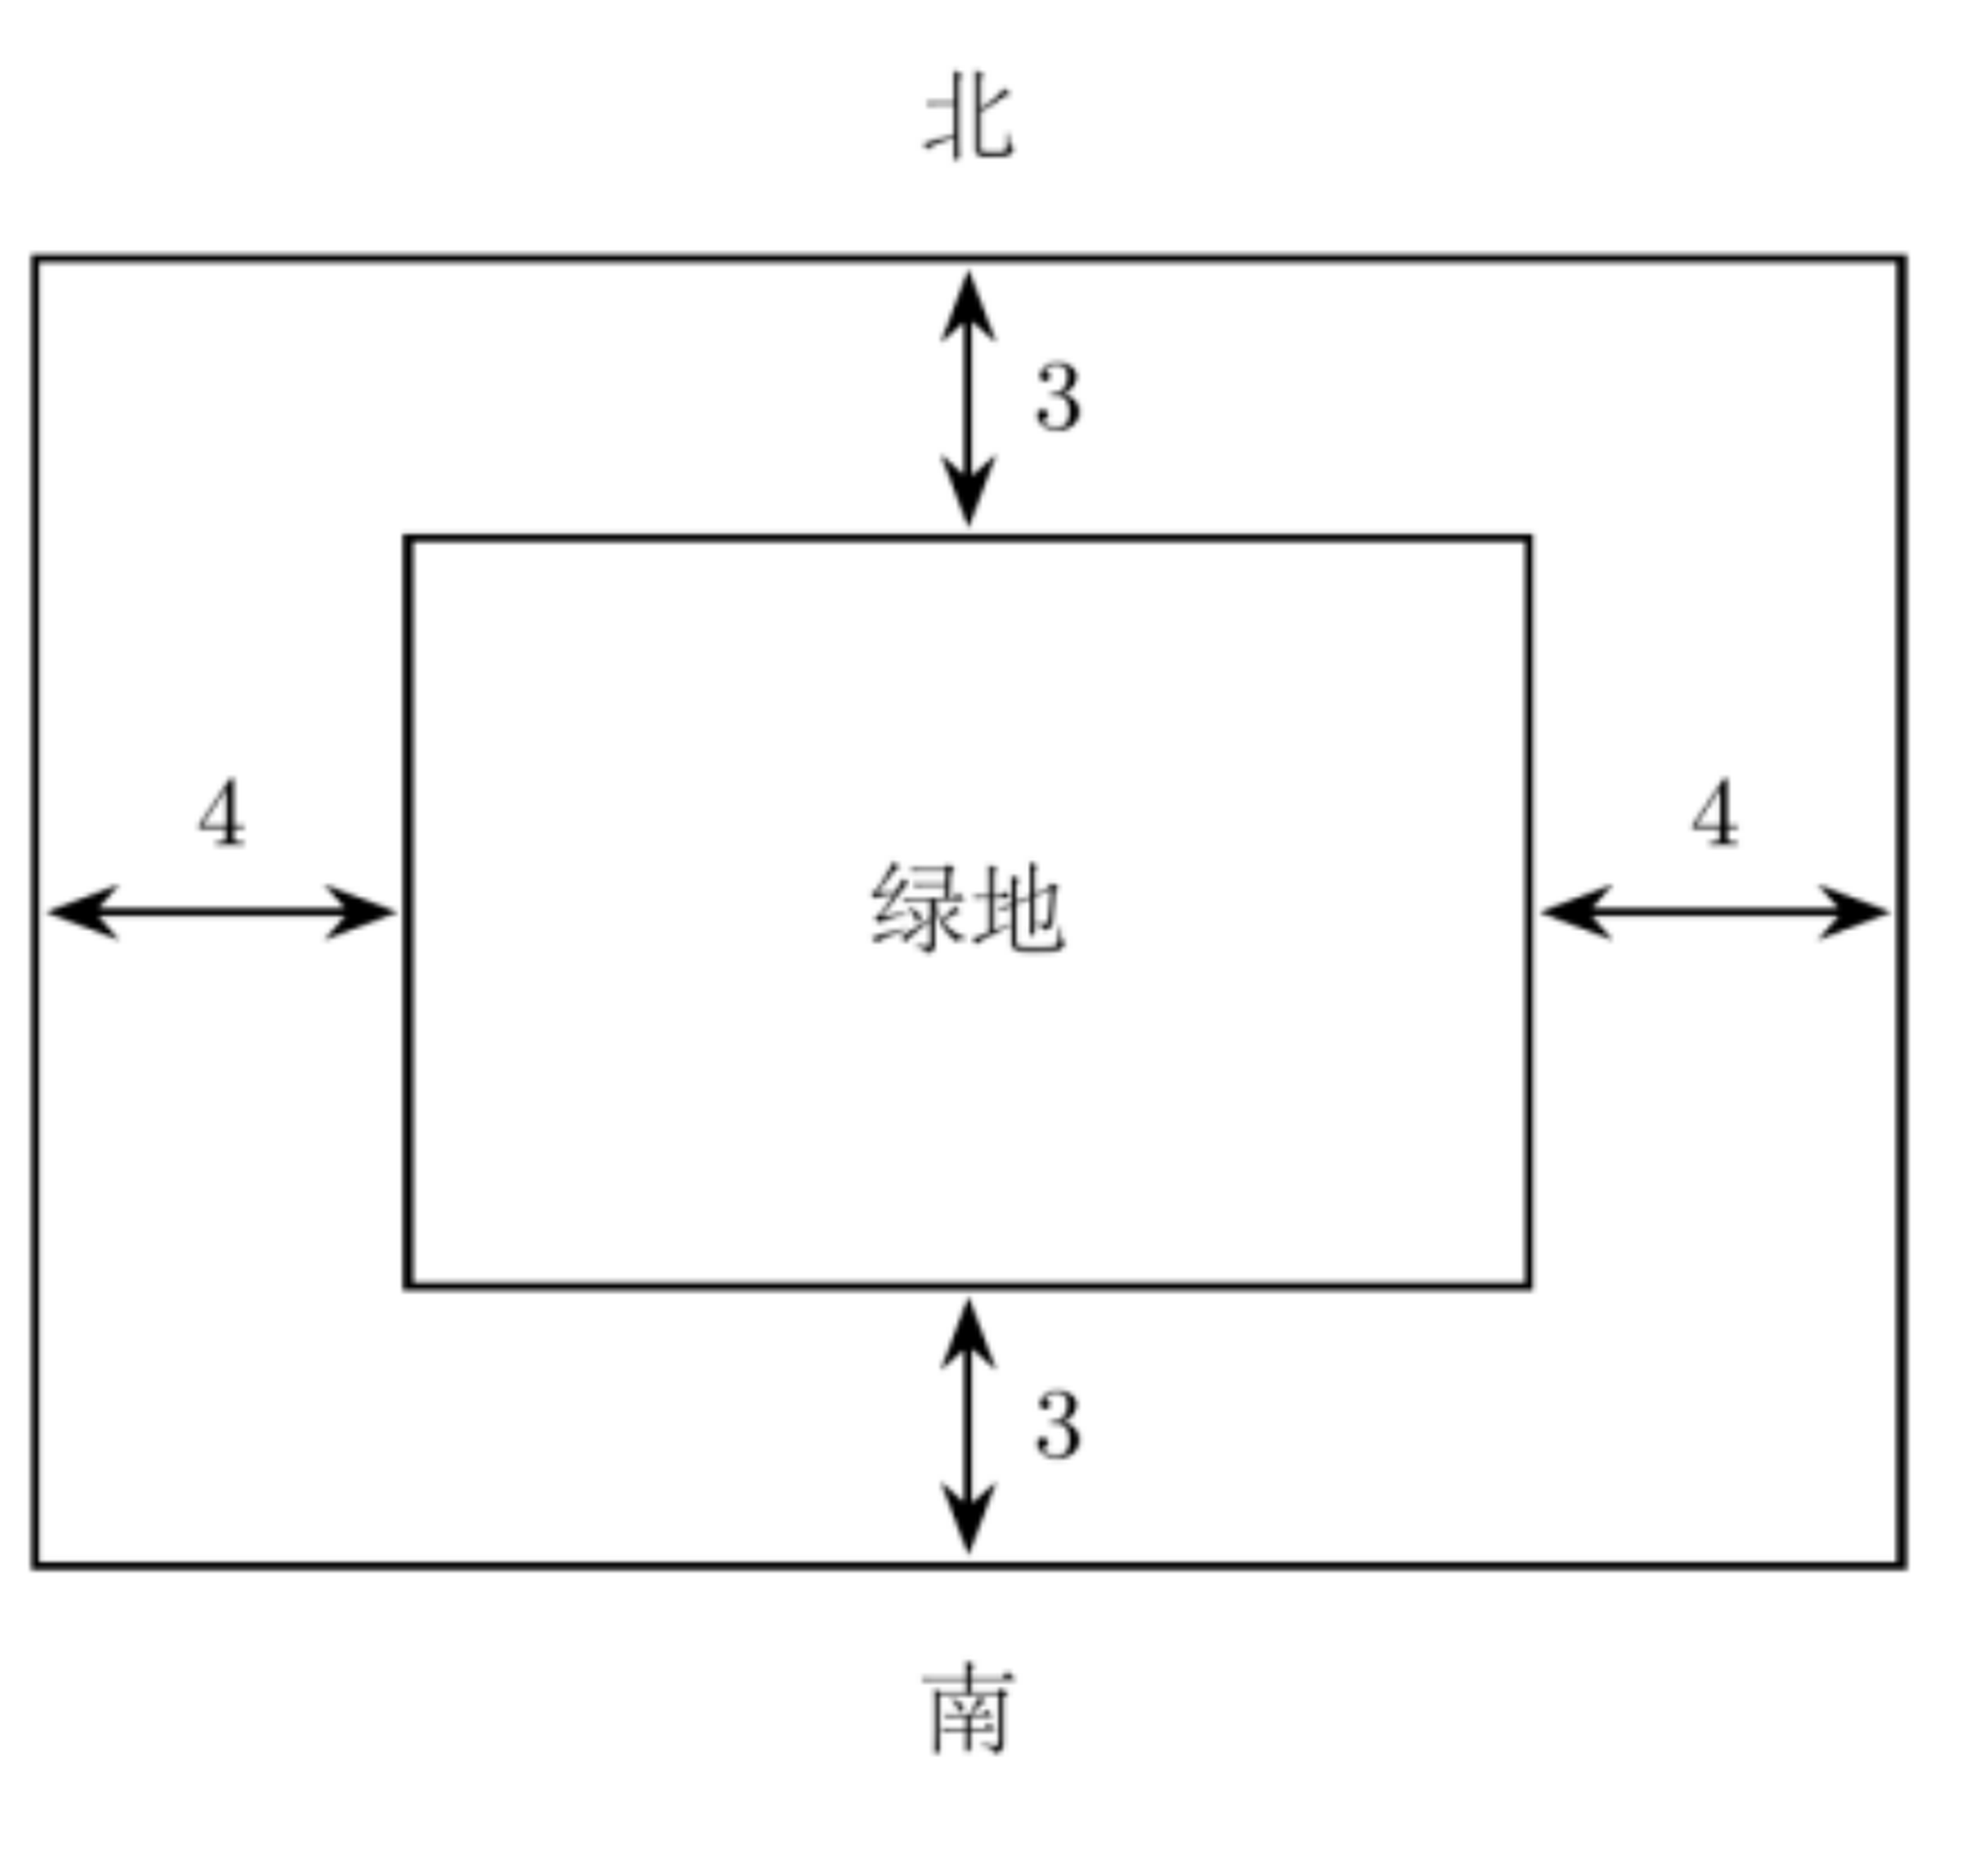
\includegraphics[width=0.32\textwidth]{figures/gao129_q19.png}
\end{center}

(1) 将 $S$ 表示为 $x$ 的函数；

(2) 试确定绿地东西方向的边长和南北方向的边长，使人行道的占地面积最小，并求出人行道的占地最小面积（结果精确到 0.1 米）

\ifanswer
\solbegin
\step{(1) 绿地南北方向的边长为 $\dfrac{1000}{x}$ 米，$x>0$.}
\step{外矩形东西、南北方向的边长分别为 $x+8$ 米、$\dfrac{1000}{x}+6$ 米.}
\step{因此 $S=(x+8)\left(\dfrac{1000}{x}+6\right)-1000=6x+\dfrac{8000}{x}+48, x>0$.}
\step{(2) 因为 $x>0,S=6x+\dfrac{8000}{x}+48\geqslant2\sqrt{6x\cdot\dfrac{8000}{x}}+48=48+80\sqrt{30}$.}
\step{等号当且仅当 $6x=\dfrac{8000}{x}$，即 $x=\dfrac{20\sqrt{30}}{3}\approx36.5$ 时成立，}
\step{此时绿地南北方向的边长为 $\dfrac{1000}{x}=\dfrac{1000}{\dfrac{20\sqrt{30}}{3}}=5\sqrt{30}\approx27.4$（米），}
\step{所以绿地东西方向、南北方向的边长分别约为 36.5 米、27.4 米时，}
\step{人行道的占地面积最小，最小面积为 $S_{min}=48+80\sqrt{30}\approx486.2$ 平方米.}
\solend
\fi

\item 已知集合 $A=\{x\mid x^2-3x+2=0\},B=\{x\mid x^2-ax+a-1=0\}$，

$C=\{x\mid x^2+2(m+1)x+m^2-5=0\}$.

(1) 若 $A=B$，求实数 $a$ 的值；

(2) 若 $B=\{1\}$，求实数 $a$ 的值；

(3) 若 $A\cap C=C$，求实数 $m$ 的取值范围.

\ifanswer
\solbegin
\step{(1) $A=\{1,2\}$，且 $x^2-ax+a-1=(x-1)(x-a+1)$，所以 $B=\{1,a-1\}$，}
\step{因此 $A=B\Leftrightarrow a-1=2\Leftrightarrow a=3$.}
\step{(2) $B=\{1\}$ 表示原方程只有一个不同的实数根，}
\step{得 $a-1=1$，即 $a=2$.}
\step{当 $a=2$ 时，原方程为 $(x-1)^2=0$，符合题意.}
\step{(3) $A\cap C=C\Leftrightarrow C\subseteq\{1,2\}$，}
\step{方程的判别式为 $\Delta=[2(m+1)]^2-4(m^2-5)=8(m+3)$.}
\step{当 $m<-3$ 时，$\Delta<0, C=\varnothing$，满足条件.}
\step{当 $m=-3$ 时，原方程为 $(x-2)^2=0, C=\{2\}$，满足条件.}
\step{当 $m>-3$ 时，方程有两个不同的实数根，必须有 $C=\{1,2\}$，}
\step{由韦达定理，$\begin{cases}-2(m+1)=1+2=3\\m^2-5=1\cdot2=2\end{cases}$，}
\step{第一式得 $m=-\dfrac52$，但此时 $m^2-5=\dfrac54\neq2$，不合题意.}
\step{因此 $m$ 的取值范围为 $(-\infty,-3]$.}
\solend
\fi

\item 设函数 $f(x)=ax^2+(1-a)x+a-2(a\in\R)$.

(1) 若关于 $x$ 的不等式 $f(x)\leqslant0$ 的解集为 $\left[0,\dfrac12\right]$，求实数 $a$ 的值；

(2) 若不等式 $f(x)\geqslant-2$ 对于实数 $a\in[-1,1]$ 时恒成立，求 $x$ 的取值范围；

(3) 解关于 $x$ 的不等式：$f(x)<a-1$.

\ifanswer
\solbegin
\step{(1) 由题意得 $0,\dfrac12$ 是方程 $ax^2+(1-a)x+a-2=0$ 的两个根，}
\step{则 $\begin{cases}0+\dfrac12=-\dfrac{1-a}{a}\\0\times\dfrac12=\dfrac{a-2}{a}\end{cases}\Rightarrow a=2$；}
\step{(2) $ax^2+(1-a)x+a-2\geqslant-2\Rightarrow a(x^2-x+1)+x\geqslant0$ 对 $a\in[-1,1]$ 恒成立，}
\step{则 $\begin{cases}-(x^2-x+1)+x\geqslant0\\(x^2-x+1)+x\geqslant0\end{cases}\Rightarrow\begin{cases}x=1\\x\in\R\end{cases}\Rightarrow x=1$，则 $x$ 的取值范围为 $\{1\}$；}
\step{(3) $f(x)<a-1$ 等价于 $ax^2+(1-a)x-1<0$，}
\step{当 $a=0$ 时，不等式可化为 $x<1$，解集为 $\{x\mid x<1\}$，}
\step{当 $a>0$ 时，不等式可化为 $(ax+1)(x-1)<0$，解集为 $\{x\mid -\dfrac1a<x<1\}$；}
\step{当 $a<0$ 时，不等式化为 $(ax+1)(x-1)<0$，}
\step{①当 $a=-1$ 时，$-\dfrac1a=1$，不等式的解集为 $\{x\mid x\neq1\}$；}
\step{②当 $-1<a<0$ 时，$-\dfrac1a>1$，不等式的解集为 $\{x\mid x<1$ 或 $x>-\dfrac1a\}$；}
\step{③当 $a<-1$ 时，$-\dfrac1a<1$，不等式的解集为 $\{x\mid x<-\dfrac1a$ 或 $x>1\}$；}
\step{综上，当 $a<-1$ 时，解集为 $\{x\mid x<-\dfrac1a$ 或 $x>1\}$；}
\step{当 $a=-1$ 时，解集为 $\{x\mid x\neq1\}$；}
\step{当 $-1<a<0$ 时，解集为 $\{x\mid x<1$ 或 $x>-\dfrac1a\}$；}
\step{当 $a=0$ 时，解集为 $\{x\mid x<1\}$；}
\step{当 $a>0$ 时，解集为 $\{x\mid -\dfrac1a<x<1\}$.}
\solend
\fi

\end{enumerate}

\end{document}
"
% 紧凑版：xelatex "\def\iscompact{1}% 高一129_立达中学_期中.tex
%   —— 高一上数学"2026-2027 年立达中学高一上期中"（试卷版/答案版）
% 试卷版：xelatex 高一129_立达中学_期中.tex
% 答案版：xelatex "\def\isanswer{1}% 高一129_立达中学_期中.tex
%   —— 高一上数学"2026-2027 年立达中学高一上期中"（试卷版/答案版）
% 试卷版：xelatex 高一129_立达中学_期中.tex
% 答案版：xelatex "\def\isanswer{1}\input{高一129_立达中学_期中.tex}"
% 紧凑版：xelatex "\def\iscompact{1}\input{高一129_立达中学_期中.tex}"
%
% 原始材料：微信公众号"魔都数学加油站"文章，作者破晓，2026-11-12 18:56 发布；
% 连载"27学年高一129"，原文标题"27学年高一129——2026-2027年上海市立达中学高一上期中"；
% 原文链接：https://mp.weixin.qq.com/s/gJhGsOBiWi7gW62u8EWLYA。
% 正文为 8 张 PNG 页（01、02、03、05、06 为 4762x6735，04、07、08 为 2560x3620），
% 题目下印有【解析】或【答案】，为讲评版。题目、解析均据原图转录；
% 卷面粉红色水印"魔都数学加油站"及公众号页脚未录入。全卷仅第 19 题有 1 幅插图。
%
% 卷首标题：原卷印作"2026-2027 年立达中学高一上期中"（公众号标题中的"上海市"
% 卷面标题行没有，本稿照卷面），年份区间按全稿惯例排 en dash；原卷未印副标题，
% 本卷为期中卷、跨集合与常用逻辑用语／不等式／函数三章，按题目内容标为
% "集合与常用逻辑用语、不等式、函数"（与 125、126 同为期中卷，口径相同）：
% 集合与逻辑见 Q3、Q4、Q13、Q20，不等式见 Q5、Q6、Q7、Q9、Q10、Q11、Q12、
% Q14、Q15、Q16、Q17、Q18、Q21，函数（含二次函数、基本不等式应用）见 Q8、Q19、Q21。
%
% 与原卷的排版差异：
%   ① 原文从第 3 题起，填空题编号为 3—12、选择题为 13—16、解答题为 17—21，本稿保留原题号；
%   ② 原卷每题下直接印【解析】／【答案】，本稿按全稿惯例置于答案版；第 3、5 题只印
%      【答案】，另提 \ans{}；第 13—16 题答案均在【解析】末句"故选 …"，题干括号内留空、
%      不另提 \ans{}；四道选择题括号内原卷均未印答案；
%   ③ 原卷未印副标题，本稿按"知识模块"口径补出（见上"卷首标题"）；
%   ④ 原卷填空横线按全稿惯例排为 \blankline[4.4em]；选择题括号排 \mbox{（\quad）}、
%      选项段前按惯例加 \keepwithprev；解答题不留作答区（原卷为讲评版，与 109—128 同）；
%   ⑤ 原卷数集排斜体 $R$，按全稿惯例改 \R；绝对值排 \lvert…\rvert，集合描述竖线排 \mid；
%      不等号按全稿惯例排 \leqslant／\geqslant；子题标号原卷一律用半角括号 (1)(2)(3)，本稿照录；
%   ⑥ 原卷第 19 题插图浮排在 Q18 解析右侧、"19."题干之上，本稿按体例就近置于 Q19
%      题干"如图所示"之后（居中 \includegraphics），图取原卷截图去水印；题前按惯例加
%      \needvspace{7cm} 守卫（照 高一120／127 成例），保证"题干 + 图"整块不被页边界切开；
%   ⑦ 原卷 Q8 解析续头印在第 2 页页首、Q17 解析续头印在第 5 页页首、Q19 题干续在第 6 页、
%      Q20 解析跨 6—7 页、Q21 解析续头印在第 8 页页首，本稿按题合并连续排版；
%      末页第 8 页为 Q21 解析的续尾，按实际印刷行单列（照 高一127 第 09 页续尾成例）。
%
% 判别式字形：第 8 题解析 $\Delta=m^2+4m>0$、第 10 题解析 $\Delta=k^2+6k=k(k+6)<0$、
%   第 20 题 (3) 解析 $\Delta=[2(m+1)]^2-4(m^2-5)=8(m+3)$ 三处原卷均排 $\Delta$
%   （等腰、高；回原图逐处放大核对、三处字形一致），照录 \Delta；全卷未出现 \triangle
%   （等边、扁）。
%
% 子集符号：第 13 题 ② $\{0,1,2\}\subseteq\{2,1,0\}$、③ $\varnothing\subseteq\{0,1,2\}$，
%   第 17 题 (2)② $B\subseteq A$、$B\subseteq(3,+\infty)$，第 20 题 (3) $C\subseteq\{1,2\}$
%   均印带下划线，照录 \subseteq；全卷未出现单线 \subset（回原图放大逐处确认）。
%
% 原卷存疑照录：
%   第 15 题解析"即 $m=4$，$n=3$ 时取等号"与题干 $\dfrac1m+n=1$、等号条件
%     $mn=\dfrac9{mn}$ 均不一致（按题应为 $n=\dfrac34$），照录、未统一；
%   第 18 题 (1) 题干"设 $M=2x^2+3x-1,N=7x-3$ 比较 $M$ 与 $N$ 两个数的大小"
%     两式间用半角逗号、且"$N=7x-3$"后无标点直接接"比较"，照录；
%   第 11 题解析"$1-x+2x-1=-(3x-2), 4x=2, x=\dfrac12$"、第 14 题解析
%     "$a=2, b=1, c=4, d=0$"、第 19 题解析"$6x+\dfrac{8000}{x}+48, x>0$"、
%     第 20 题解析"$\Delta<0, C=\varnothing$"与"$(x-2)^2=0, C=\{2\}$"、
%     第 12 题解析"$(x+y)^2=3+t\geqslant0,(x-y)^2=3-3t\geqslant0$"等处数学式内
%     用半角逗号，照录；
%   第 19 题题干"如图所示（图中单位：米）设绿地东西方向的边长为 $x$"在右括号后
%     无标点直接续"设"，照录；
%   第 21 题 (3) 解析先按 $a>0$、$a=0$、$a<0$ 分述解集，又在"综上"处重列全部
%     五类（含已给出的 $a>0$、$a=0$），照录；
%   第 21 题 (2) 题干与解析均作 $f(x)\geqslant-2$（与 $a(x^2-x+1)+x\geqslant0$ 相符），
%     照录，勿误读为 $f(x)\geqslant2$。
%
% 行数复核：逐题数 \step 条数，合计 93 条（Q3：0；Q4：2；Q5：0；Q6：3；Q7：3；
% Q8：2；Q9：4；Q10：3；Q11：5；Q12：5；Q13：1；Q14：3；Q15：3；Q16：7；
% Q17：7；Q18：8；Q19：8；Q20：13；Q21：16），与原卷印刷行逐题相等
% （cases 块作一个印刷行计）。第 3、5 题只印【答案】，提 \ans{}，不计入 \step 账；
% 四道选择题答案均在解析末句，括号内留空、不另提 \ans{}。
%
\documentclass[a4paper,11pt]{article}
\usepackage{common}

\begin{document}

\examtitlest[3]{2026--2027 年立达中学高一上期中}{集合与常用逻辑用语、不等式、函数}

\bigsec{一、填空题}

\begin{enumerate}
\setcounter{enumi}{2}

\item 若 $A=\{x\mid -3<x\leqslant2\},B=\{x\mid 1<x\leqslant3\}$，则 $A\cup B=$\blankline[4.4em].

\ifanswer
\ans{$(-3,3]$}
\fi

\item 若 $A$ 是 $B$ 的必要非充分条件，$B$ 是 $C$ 的充要条件，$C$ 是 $D$ 的必要非充分条件，则 $D$ 是 $A$ 的\blankline[4.4em]条件.

\ifanswer
\solbegin
\step{$D\Rightarrow C\Leftrightarrow B\Rightarrow A$，且 $A\nRightarrow B$，因此 $D\Rightarrow A$ 且 $A\nRightarrow D$，}
\step{故 $D$ 是 $A$ 的充分非必要条件.}
\solend
\fi

\item 不等式 $\dfrac1x<1$ 的解集为\blankline[4.4em].

\ifanswer
\ans{$(-\infty,0)\cup(1,+\infty)$}
\fi

\item 已知正实数 $x$、$y$ 满足 $2x+y=2$，则 $xy$ 的最大值为\blankline[4.4em].

\ifanswer
\solbegin
\step{因为 $x>0$，$y>0$，所以 $2x+y\geqslant2\sqrt{2xy}$（当且仅当 $2x=y$ 时，取等号），}
\step{又因为 $2x+y=2$，所以 $2\geqslant2\sqrt{2xy}$（当且仅当 $2x=y$ 时，取等号），}
\step{即 $xy\leqslant\dfrac12$，则 $xy$ 的最大值为 $\dfrac12$.}
\solend
\fi

\item 已知 $x\in\R$，函数 $y=\lvert x+2\rvert+\lvert x-3\rvert$ 的最小值为\blankline[4.4em].

\ifanswer
\solbegin
\step{由 $\lvert x+2\rvert+\lvert x-3\rvert\geqslant\lvert(x+2)-(x-3)\rvert=5$，}
\step{当且仅当 $(x+2)(x-3)\leqslant0$，即 $-2\leqslant x\leqslant3$ 时，上式取等号，}
\step{则函数 $y=\lvert x+2\rvert+\lvert x-3\rvert$ 的最小值是 5.}
\solend
\fi

\item 已知实系数一元二次方程 $x^2+mx-m=0$ 的两根分别为 $x_1,x_2$，且 $\lvert x_1-x_2\rvert=\sqrt{21}$，实数 $m$ 的值为\blankline[4.4em].

\ifanswer
\solbegin
\step{由题意得 $\Delta=m^2+4m>0$，解得 $m>0$ 或 $m<-4,x_1+x_2=-m,x_1x_2=-m$，}
\step{则 $\lvert x_1-x_2\rvert=\sqrt{(x_1+x_2)^2-4x_1x_2}=\sqrt{m^2+4m}=\sqrt{21}$，解得 $m=-7$ 或 $3$.}
\solend
\fi

\item 已知不等式 $ax^2-5x+b>0$ 的解集是 $\{x\mid -3<x<-2\}$，则不等式 $bx^2-5x+a>0$ 的解集是\blankline[4.4em].

\ifanswer
\solbegin
\step{$ax^2-5x+b=a(x+3)(x+2)$，比较系数得 $5a=-5,b=6a$，}
\step{即 $a=-1,b=-6$.}
\step{$bx^2-5x+a>0\Leftrightarrow(3x+1)(2x+1)<0\Leftrightarrow-\dfrac12<x<-\dfrac13$，}
\step{故解集为 $\left\{x\mid -\dfrac12<x<-\dfrac13\right\}$.}
\solend
\fi

\item 不等式 $4kx^2+kx-\dfrac38<0$ 对于一切实数 $x$ 都成立，则实数 $k$ 的取值范围是\blankline[4.4em].

\ifanswer
\solbegin
\step{$k=0$ 时，不等式恒成立；}
\step{$k\neq0$ 时，须 $4k<0$ 且 $\Delta=k^2+6k=k(k+6)<0$，解得 $-6<k<0$.}
\step{因此 $k\in(-6,0]$.}
\solend
\fi

\item 设 $x\in\R$，方程 $\lvert 1-x\rvert+\lvert 2x-1\rvert=\lvert 3x-2\rvert$ 的解集为\blankline[4.4em].

\ifanswer
\solbegin
\step{当 $x\leqslant\dfrac12$ 时，方程化为 $1-x-(2x-1)=-(3x-2)$，$2-3x=-3x+2$，恒成立，}
\step{当 $\dfrac12<x\leqslant\dfrac23$ 时，方程化为 $1-x+2x-1=-(3x-2), 4x=2, x=\dfrac12$，不合题意，}
\step{当 $\dfrac23<x\leqslant1$ 时，方程化为 $1-x+2x-1=3x-2$，$2x=2$，解得 $x=1$，}
\step{当 $x>1$ 时，方程化为 $-(1-x)+2x-1=3x-2$，$3x-2=3x-2$，恒成立，}
\step{综上所述，$\lvert 1-x\rvert+\lvert 2x-1\rvert=\lvert 3x-2\rvert$ 的解集为 $\left(-\infty,\dfrac12\right]\cup[1,+\infty)$.}
\solend
\fi

\item 已知非零实数 $x,y$ 满足 $x^2+xy+y^2=3$，则 $x^2-xy+y^2$ 的取值范围是\blankline[4.4em].

\ifanswer
\solbegin
\step{令 $t=xy\neq0$，由 $(x+y)^2=3+t\geqslant0,(x-y)^2=3-3t\geqslant0$，}
\step{得 $t\in[-3,0)\cup(0,1]$.}
\step{对上述任意 $t$，联立 $x+y=\sqrt{3+t},x-y=\sqrt{3-3t}$，所得 $x,y$ 满足原条件，}
\step{因此上述 $t$ 均可取到.}
\step{于是 $x^2-xy+y^2=3-2t$ 的取值范围为 $[1,3)\cup(3,9]$.}
\solend
\fi

\end{enumerate}

\bigsec{二、选择题}

\begin{enumerate}
\setcounter{enumi}{12}

\item 下列各式中，正确的个数是\mbox{（\quad）}

① $\{0\}\in\{0,1,2\}$；② $\{0,1,2\}\subseteq\{2,1,0\}$；③ $\varnothing\subseteq\{0,1,2\}$；④ $\varnothing=\{0\}$；⑤ $\{0,1\}=\{(0,1)\}$；

⑥ $0=\{0\}$.

\keepwithprev
A. $1$\qquad\qquad B. $2$\qquad\qquad C. $3$\qquad\qquad D. $4$

\ifanswer
\solbegin
\step{①不正确，②正确，③正确，④不正确，⑤不正确，⑥不正确. 故选 $B$.}
\solend
\fi

\item 下列四个命题中，为真命题的是\mbox{（\quad）}

\keepwithprev
A. 若 $a>b$，则 $ac^2>bc^2$\qquad\qquad B. 若 $a>b,c>d$，则 $a-c>b-d$

C. 若 $ac^2>bc^2$，则 $a>b$\qquad\qquad D. 若 $a>b$，则 $\dfrac1a<\dfrac1b$

\ifanswer
\solbegin
\step{C 中，$(a-b)c^2>0$，必有 $c^2>0$ 且 $a-b>0$，即 $a>b$.}
\step{A 取 $c=0$；B 取 $a=2, b=1, c=4, d=0$；D 取 $a=1, b=-1$，均不成立.}
\step{故选 $C$.}
\solend
\fi

\item 已知 $m$、$n\in(0,+\infty)$，$\dfrac1m+n=1$，则 $m+\dfrac9n$ 的最小值为\mbox{（\quad）}

\keepwithprev
A. $13$\qquad\qquad B. $16$\qquad\qquad C. $3$\qquad\qquad D. $6$

\ifanswer
\solbegin
\step{因为 $m$、$n\in(0,+\infty)$，$\dfrac1m+n=1$，}
\step{所以 $m+\dfrac9n=(m+\dfrac9n)(\dfrac1m+n)=10+mn+\dfrac9{mn}\geqslant10+2\sqrt{mn\cdot\dfrac9{mn}}=16$，}
\step{当且仅当 $mn=\dfrac9{mn}$，即 $m=4$，$n=3$ 时取等号. 故选 $B$.}
\solend
\fi

\item 下列不等式：① $\left\lvert x+\dfrac1x\right\rvert\geqslant2$；② $x^2+2x+1>0$；③ $\lvert x\rvert+\lvert x-1\rvert\geqslant1$；④ $\dfrac{x}{x^2+x+1}<1$；

解集为 $\R$ 的不等式的个数是\mbox{（\quad）}

\keepwithprev
A. $0$\qquad\qquad B. $1$\qquad\qquad C. $2$\qquad\qquad D. $3$

\ifanswer
\solbegin
\step{对于①，当 $x=0$ 时，$\dfrac1x$ 无意义，故 $\left\lvert x+\dfrac1x\right\rvert\geqslant2$ 的解集不是 $\R$，错误；}
\step{对于②，$x^2+2x+1=(x+1)^2\geqslant0$，当 $x=-1$ 取到等号，解集不是 $\R$，故错误；}
\step{对于③，$\lvert x\rvert+\lvert x-1\rvert\geqslant\lvert x-(x-1)\rvert=1$，当 $x(x-1)\leqslant0$ 时取等号，解集为 $\R$，}
\step{故正确；}
\step{对于④，由于 $x^2+x+1>0$ 恒成立，}
\step{故 $\dfrac{x}{x^2+x+1}<1$ 等价于 $x<x^2+x+1\Rightarrow x^2+1>0$ 恒成立，故解集为 $\R$，正确，}
\step{故正确的有③④，故选 $C$.}
\solend
\fi

\end{enumerate}

\bigsec{三、解答题}

\begin{enumerate}
\setcounter{enumi}{16}

\item (1) 解不等式组 $\begin{cases}\dfrac{x+3}{x+1}\leqslant2\\\lvert 2x-3\rvert\leqslant2\end{cases}$.

(2) 已知集合 $A=\{x\mid -x+3<0\},B=\{x\mid a\leqslant x\leqslant a+3\}$.

①当 $a=2$，求集合 $A\cap B$；

②若 $A\cup B=A$，求实数 $a$ 的取值范围.

\ifanswer
\solbegin
\step{(1) 由 $\begin{cases}\dfrac{x+3}{x+1}\leqslant2\\\lvert 2x-3\rvert\leqslant2\end{cases}$ 得 $\begin{cases}\dfrac{x+3-2x-2}{x+1}\leqslant0\\-2\leqslant2x-3\leqslant2\end{cases}$，即 $\begin{cases}\dfrac{-x+1}{x+1}\leqslant0\\1\leqslant2x\leqslant5\end{cases}$，则 $\begin{cases}\dfrac{x-1}{x+1}\geqslant0\\\dfrac12\leqslant x\leqslant\dfrac52\end{cases}$，}
\step{解得 $1\leqslant x\leqslant\dfrac52$，即原不等式组的解集为 $\left[1,\dfrac52\right]$.}
\step{(2) $-x+3<0\Leftrightarrow x>3$，所以 $A=(3,+\infty)$.}
\step{①当 $a=2$ 时，$B=[2,5], A\cap B=(3,+\infty)\cap[2,5]=(3,5]$.}
\step{②$A\cup B=A\Leftrightarrow B\subseteq A$.}
\step{因为 $B=[a,a+3]$，且左端点 $a\in B$，所以 $B\subseteq(3,+\infty)\Leftrightarrow a>3$，}
\step{实数 $a$ 的取值范围为 $(3,+\infty)$.}
\solend
\fi

\item (1) 设 $M=2x^2+3x-1,N=7x-3$ 比较 $M$ 与 $N$ 两个数的大小.

(2) 解关于 $x$ 的不等式：$x^2-(a+3)x+3a<0$，$a\in\R$.

\ifanswer
\solbegin
\step{(1) $M-N=2x^2+3x-1-(7x-3)=2(x-1)^2$.}
\step{$x=1$ 时，$M-N=0$，即 $M=N$.}
\step{$x\neq1$ 时，$M-N>0$，即 $M>N$.}
\step{(2) 不等式 $x^2-(a+3)x+3a<0$ 可化为 $(x-3)(x-a)<0$，}
\step{不等式对应方程的解为 $a$ 和 3，}
\step{当 $a<3$ 时，不等式 $x^2-(a+3)x+3a<0$ 的解集为 $(a,3)$，}
\step{当 $a=3$ 时，不等式 $x^2-(a+3)x+3a<0$ 的解集为 $\varnothing$，}
\step{当 $a>3$ 时，不等式 $x^2-(a+3)x+3a<0$ 的解集为 $(3,a)$.}
\solend
\fi

% 第 19 题是"题干 + 图"约 7cm 的一整块，答案版实测断点落在题干之后（图被推到次页页首），
% 照 高一120／127 成例在题前先量一次页高，不够就把"题干 + 图"整块一起挪到次页。
\needvspace{7cm}
\item 某新建居民小区欲建一面积为 1000 平方米的矩形绿地，在绿地四周铺设人行道，设计要求绿地南北两侧人行道宽 3 米，东西两侧人行道宽 4 米，如图所示（图中单位：米）设绿地东西方向的边长为 $x$，人行道的占地面积为 $S$.

\begin{center}
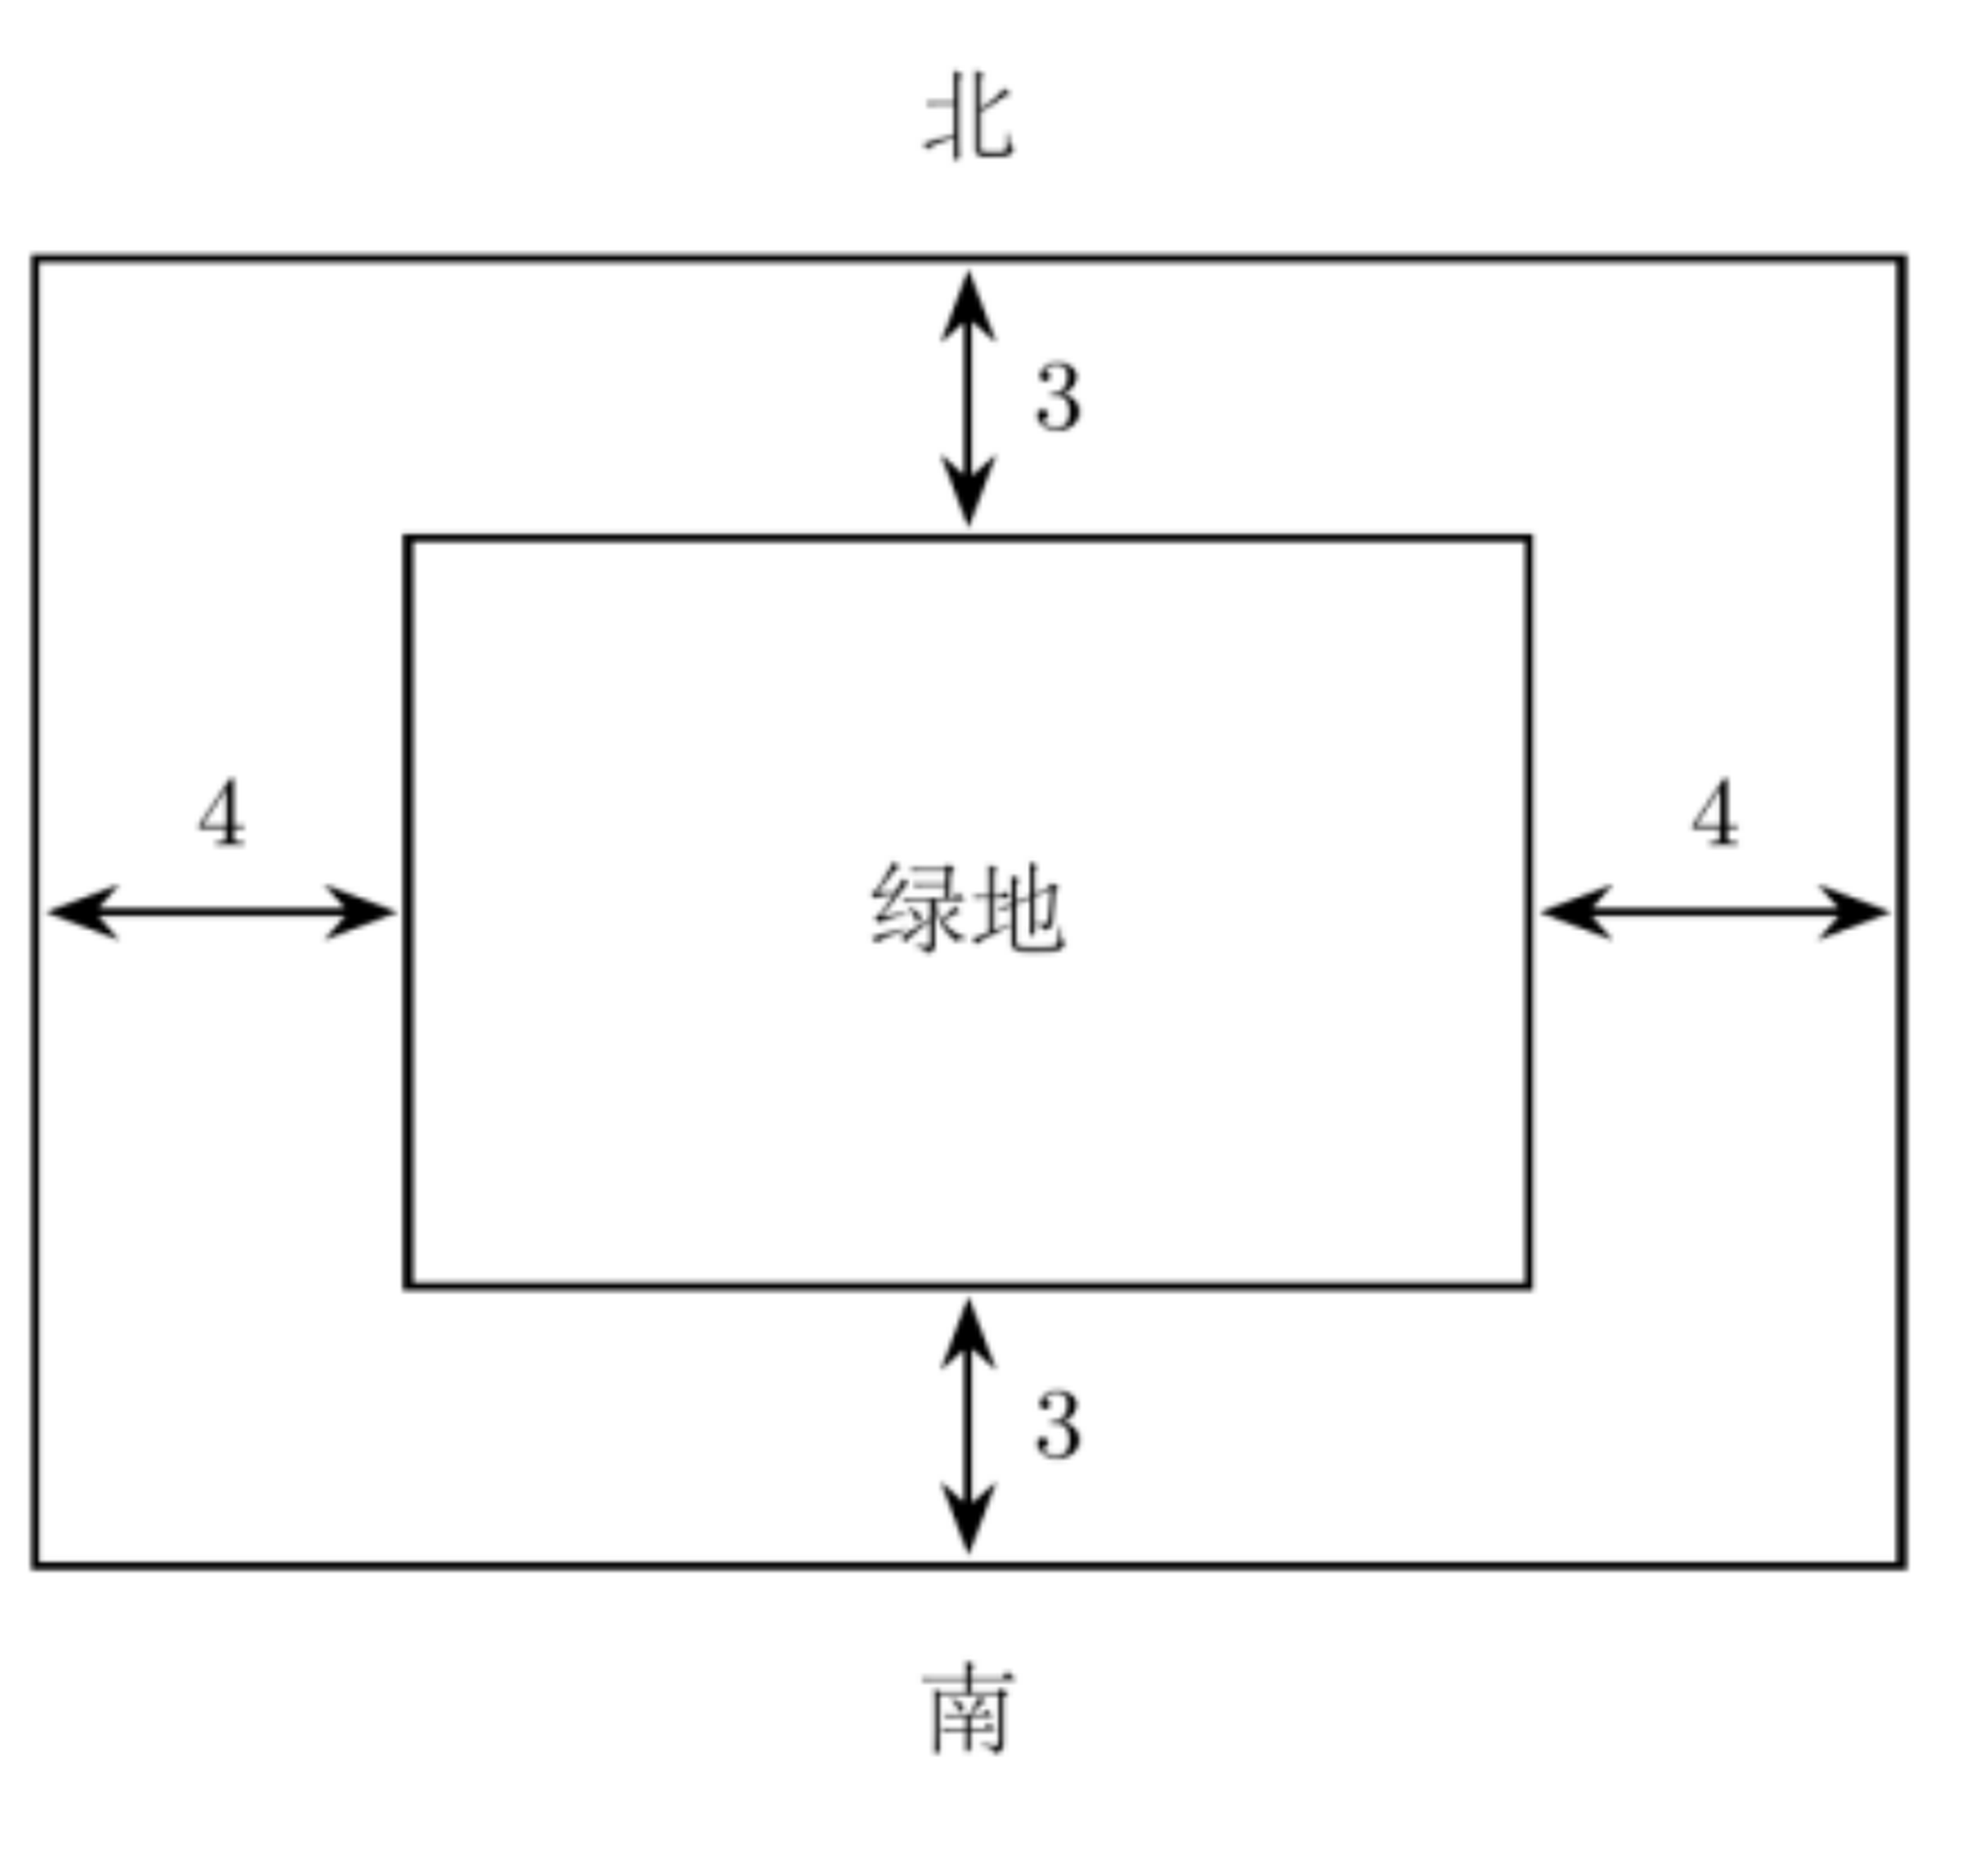
\includegraphics[width=0.32\textwidth]{figures/gao129_q19.png}
\end{center}

(1) 将 $S$ 表示为 $x$ 的函数；

(2) 试确定绿地东西方向的边长和南北方向的边长，使人行道的占地面积最小，并求出人行道的占地最小面积（结果精确到 0.1 米）

\ifanswer
\solbegin
\step{(1) 绿地南北方向的边长为 $\dfrac{1000}{x}$ 米，$x>0$.}
\step{外矩形东西、南北方向的边长分别为 $x+8$ 米、$\dfrac{1000}{x}+6$ 米.}
\step{因此 $S=(x+8)\left(\dfrac{1000}{x}+6\right)-1000=6x+\dfrac{8000}{x}+48, x>0$.}
\step{(2) 因为 $x>0,S=6x+\dfrac{8000}{x}+48\geqslant2\sqrt{6x\cdot\dfrac{8000}{x}}+48=48+80\sqrt{30}$.}
\step{等号当且仅当 $6x=\dfrac{8000}{x}$，即 $x=\dfrac{20\sqrt{30}}{3}\approx36.5$ 时成立，}
\step{此时绿地南北方向的边长为 $\dfrac{1000}{x}=\dfrac{1000}{\dfrac{20\sqrt{30}}{3}}=5\sqrt{30}\approx27.4$（米），}
\step{所以绿地东西方向、南北方向的边长分别约为 36.5 米、27.4 米时，}
\step{人行道的占地面积最小，最小面积为 $S_{min}=48+80\sqrt{30}\approx486.2$ 平方米.}
\solend
\fi

\item 已知集合 $A=\{x\mid x^2-3x+2=0\},B=\{x\mid x^2-ax+a-1=0\}$，

$C=\{x\mid x^2+2(m+1)x+m^2-5=0\}$.

(1) 若 $A=B$，求实数 $a$ 的值；

(2) 若 $B=\{1\}$，求实数 $a$ 的值；

(3) 若 $A\cap C=C$，求实数 $m$ 的取值范围.

\ifanswer
\solbegin
\step{(1) $A=\{1,2\}$，且 $x^2-ax+a-1=(x-1)(x-a+1)$，所以 $B=\{1,a-1\}$，}
\step{因此 $A=B\Leftrightarrow a-1=2\Leftrightarrow a=3$.}
\step{(2) $B=\{1\}$ 表示原方程只有一个不同的实数根，}
\step{得 $a-1=1$，即 $a=2$.}
\step{当 $a=2$ 时，原方程为 $(x-1)^2=0$，符合题意.}
\step{(3) $A\cap C=C\Leftrightarrow C\subseteq\{1,2\}$，}
\step{方程的判别式为 $\Delta=[2(m+1)]^2-4(m^2-5)=8(m+3)$.}
\step{当 $m<-3$ 时，$\Delta<0, C=\varnothing$，满足条件.}
\step{当 $m=-3$ 时，原方程为 $(x-2)^2=0, C=\{2\}$，满足条件.}
\step{当 $m>-3$ 时，方程有两个不同的实数根，必须有 $C=\{1,2\}$，}
\step{由韦达定理，$\begin{cases}-2(m+1)=1+2=3\\m^2-5=1\cdot2=2\end{cases}$，}
\step{第一式得 $m=-\dfrac52$，但此时 $m^2-5=\dfrac54\neq2$，不合题意.}
\step{因此 $m$ 的取值范围为 $(-\infty,-3]$.}
\solend
\fi

\item 设函数 $f(x)=ax^2+(1-a)x+a-2(a\in\R)$.

(1) 若关于 $x$ 的不等式 $f(x)\leqslant0$ 的解集为 $\left[0,\dfrac12\right]$，求实数 $a$ 的值；

(2) 若不等式 $f(x)\geqslant-2$ 对于实数 $a\in[-1,1]$ 时恒成立，求 $x$ 的取值范围；

(3) 解关于 $x$ 的不等式：$f(x)<a-1$.

\ifanswer
\solbegin
\step{(1) 由题意得 $0,\dfrac12$ 是方程 $ax^2+(1-a)x+a-2=0$ 的两个根，}
\step{则 $\begin{cases}0+\dfrac12=-\dfrac{1-a}{a}\\0\times\dfrac12=\dfrac{a-2}{a}\end{cases}\Rightarrow a=2$；}
\step{(2) $ax^2+(1-a)x+a-2\geqslant-2\Rightarrow a(x^2-x+1)+x\geqslant0$ 对 $a\in[-1,1]$ 恒成立，}
\step{则 $\begin{cases}-(x^2-x+1)+x\geqslant0\\(x^2-x+1)+x\geqslant0\end{cases}\Rightarrow\begin{cases}x=1\\x\in\R\end{cases}\Rightarrow x=1$，则 $x$ 的取值范围为 $\{1\}$；}
\step{(3) $f(x)<a-1$ 等价于 $ax^2+(1-a)x-1<0$，}
\step{当 $a=0$ 时，不等式可化为 $x<1$，解集为 $\{x\mid x<1\}$，}
\step{当 $a>0$ 时，不等式可化为 $(ax+1)(x-1)<0$，解集为 $\{x\mid -\dfrac1a<x<1\}$；}
\step{当 $a<0$ 时，不等式化为 $(ax+1)(x-1)<0$，}
\step{①当 $a=-1$ 时，$-\dfrac1a=1$，不等式的解集为 $\{x\mid x\neq1\}$；}
\step{②当 $-1<a<0$ 时，$-\dfrac1a>1$，不等式的解集为 $\{x\mid x<1$ 或 $x>-\dfrac1a\}$；}
\step{③当 $a<-1$ 时，$-\dfrac1a<1$，不等式的解集为 $\{x\mid x<-\dfrac1a$ 或 $x>1\}$；}
\step{综上，当 $a<-1$ 时，解集为 $\{x\mid x<-\dfrac1a$ 或 $x>1\}$；}
\step{当 $a=-1$ 时，解集为 $\{x\mid x\neq1\}$；}
\step{当 $-1<a<0$ 时，解集为 $\{x\mid x<1$ 或 $x>-\dfrac1a\}$；}
\step{当 $a=0$ 时，解集为 $\{x\mid x<1\}$；}
\step{当 $a>0$ 时，解集为 $\{x\mid -\dfrac1a<x<1\}$.}
\solend
\fi

\end{enumerate}

\end{document}
"
% 紧凑版：xelatex "\def\iscompact{1}% 高一129_立达中学_期中.tex
%   —— 高一上数学"2026-2027 年立达中学高一上期中"（试卷版/答案版）
% 试卷版：xelatex 高一129_立达中学_期中.tex
% 答案版：xelatex "\def\isanswer{1}\input{高一129_立达中学_期中.tex}"
% 紧凑版：xelatex "\def\iscompact{1}\input{高一129_立达中学_期中.tex}"
%
% 原始材料：微信公众号"魔都数学加油站"文章，作者破晓，2026-11-12 18:56 发布；
% 连载"27学年高一129"，原文标题"27学年高一129——2026-2027年上海市立达中学高一上期中"；
% 原文链接：https://mp.weixin.qq.com/s/gJhGsOBiWi7gW62u8EWLYA。
% 正文为 8 张 PNG 页（01、02、03、05、06 为 4762x6735，04、07、08 为 2560x3620），
% 题目下印有【解析】或【答案】，为讲评版。题目、解析均据原图转录；
% 卷面粉红色水印"魔都数学加油站"及公众号页脚未录入。全卷仅第 19 题有 1 幅插图。
%
% 卷首标题：原卷印作"2026-2027 年立达中学高一上期中"（公众号标题中的"上海市"
% 卷面标题行没有，本稿照卷面），年份区间按全稿惯例排 en dash；原卷未印副标题，
% 本卷为期中卷、跨集合与常用逻辑用语／不等式／函数三章，按题目内容标为
% "集合与常用逻辑用语、不等式、函数"（与 125、126 同为期中卷，口径相同）：
% 集合与逻辑见 Q3、Q4、Q13、Q20，不等式见 Q5、Q6、Q7、Q9、Q10、Q11、Q12、
% Q14、Q15、Q16、Q17、Q18、Q21，函数（含二次函数、基本不等式应用）见 Q8、Q19、Q21。
%
% 与原卷的排版差异：
%   ① 原文从第 3 题起，填空题编号为 3—12、选择题为 13—16、解答题为 17—21，本稿保留原题号；
%   ② 原卷每题下直接印【解析】／【答案】，本稿按全稿惯例置于答案版；第 3、5 题只印
%      【答案】，另提 \ans{}；第 13—16 题答案均在【解析】末句"故选 …"，题干括号内留空、
%      不另提 \ans{}；四道选择题括号内原卷均未印答案；
%   ③ 原卷未印副标题，本稿按"知识模块"口径补出（见上"卷首标题"）；
%   ④ 原卷填空横线按全稿惯例排为 \blankline[4.4em]；选择题括号排 \mbox{（\quad）}、
%      选项段前按惯例加 \keepwithprev；解答题不留作答区（原卷为讲评版，与 109—128 同）；
%   ⑤ 原卷数集排斜体 $R$，按全稿惯例改 \R；绝对值排 \lvert…\rvert，集合描述竖线排 \mid；
%      不等号按全稿惯例排 \leqslant／\geqslant；子题标号原卷一律用半角括号 (1)(2)(3)，本稿照录；
%   ⑥ 原卷第 19 题插图浮排在 Q18 解析右侧、"19."题干之上，本稿按体例就近置于 Q19
%      题干"如图所示"之后（居中 \includegraphics），图取原卷截图去水印；题前按惯例加
%      \needvspace{7cm} 守卫（照 高一120／127 成例），保证"题干 + 图"整块不被页边界切开；
%   ⑦ 原卷 Q8 解析续头印在第 2 页页首、Q17 解析续头印在第 5 页页首、Q19 题干续在第 6 页、
%      Q20 解析跨 6—7 页、Q21 解析续头印在第 8 页页首，本稿按题合并连续排版；
%      末页第 8 页为 Q21 解析的续尾，按实际印刷行单列（照 高一127 第 09 页续尾成例）。
%
% 判别式字形：第 8 题解析 $\Delta=m^2+4m>0$、第 10 题解析 $\Delta=k^2+6k=k(k+6)<0$、
%   第 20 题 (3) 解析 $\Delta=[2(m+1)]^2-4(m^2-5)=8(m+3)$ 三处原卷均排 $\Delta$
%   （等腰、高；回原图逐处放大核对、三处字形一致），照录 \Delta；全卷未出现 \triangle
%   （等边、扁）。
%
% 子集符号：第 13 题 ② $\{0,1,2\}\subseteq\{2,1,0\}$、③ $\varnothing\subseteq\{0,1,2\}$，
%   第 17 题 (2)② $B\subseteq A$、$B\subseteq(3,+\infty)$，第 20 题 (3) $C\subseteq\{1,2\}$
%   均印带下划线，照录 \subseteq；全卷未出现单线 \subset（回原图放大逐处确认）。
%
% 原卷存疑照录：
%   第 15 题解析"即 $m=4$，$n=3$ 时取等号"与题干 $\dfrac1m+n=1$、等号条件
%     $mn=\dfrac9{mn}$ 均不一致（按题应为 $n=\dfrac34$），照录、未统一；
%   第 18 题 (1) 题干"设 $M=2x^2+3x-1,N=7x-3$ 比较 $M$ 与 $N$ 两个数的大小"
%     两式间用半角逗号、且"$N=7x-3$"后无标点直接接"比较"，照录；
%   第 11 题解析"$1-x+2x-1=-(3x-2), 4x=2, x=\dfrac12$"、第 14 题解析
%     "$a=2, b=1, c=4, d=0$"、第 19 题解析"$6x+\dfrac{8000}{x}+48, x>0$"、
%     第 20 题解析"$\Delta<0, C=\varnothing$"与"$(x-2)^2=0, C=\{2\}$"、
%     第 12 题解析"$(x+y)^2=3+t\geqslant0,(x-y)^2=3-3t\geqslant0$"等处数学式内
%     用半角逗号，照录；
%   第 19 题题干"如图所示（图中单位：米）设绿地东西方向的边长为 $x$"在右括号后
%     无标点直接续"设"，照录；
%   第 21 题 (3) 解析先按 $a>0$、$a=0$、$a<0$ 分述解集，又在"综上"处重列全部
%     五类（含已给出的 $a>0$、$a=0$），照录；
%   第 21 题 (2) 题干与解析均作 $f(x)\geqslant-2$（与 $a(x^2-x+1)+x\geqslant0$ 相符），
%     照录，勿误读为 $f(x)\geqslant2$。
%
% 行数复核：逐题数 \step 条数，合计 93 条（Q3：0；Q4：2；Q5：0；Q6：3；Q7：3；
% Q8：2；Q9：4；Q10：3；Q11：5；Q12：5；Q13：1；Q14：3；Q15：3；Q16：7；
% Q17：7；Q18：8；Q19：8；Q20：13；Q21：16），与原卷印刷行逐题相等
% （cases 块作一个印刷行计）。第 3、5 题只印【答案】，提 \ans{}，不计入 \step 账；
% 四道选择题答案均在解析末句，括号内留空、不另提 \ans{}。
%
\documentclass[a4paper,11pt]{article}
\usepackage{common}

\begin{document}

\examtitlest[3]{2026--2027 年立达中学高一上期中}{集合与常用逻辑用语、不等式、函数}

\bigsec{一、填空题}

\begin{enumerate}
\setcounter{enumi}{2}

\item 若 $A=\{x\mid -3<x\leqslant2\},B=\{x\mid 1<x\leqslant3\}$，则 $A\cup B=$\blankline[4.4em].

\ifanswer
\ans{$(-3,3]$}
\fi

\item 若 $A$ 是 $B$ 的必要非充分条件，$B$ 是 $C$ 的充要条件，$C$ 是 $D$ 的必要非充分条件，则 $D$ 是 $A$ 的\blankline[4.4em]条件.

\ifanswer
\solbegin
\step{$D\Rightarrow C\Leftrightarrow B\Rightarrow A$，且 $A\nRightarrow B$，因此 $D\Rightarrow A$ 且 $A\nRightarrow D$，}
\step{故 $D$ 是 $A$ 的充分非必要条件.}
\solend
\fi

\item 不等式 $\dfrac1x<1$ 的解集为\blankline[4.4em].

\ifanswer
\ans{$(-\infty,0)\cup(1,+\infty)$}
\fi

\item 已知正实数 $x$、$y$ 满足 $2x+y=2$，则 $xy$ 的最大值为\blankline[4.4em].

\ifanswer
\solbegin
\step{因为 $x>0$，$y>0$，所以 $2x+y\geqslant2\sqrt{2xy}$（当且仅当 $2x=y$ 时，取等号），}
\step{又因为 $2x+y=2$，所以 $2\geqslant2\sqrt{2xy}$（当且仅当 $2x=y$ 时，取等号），}
\step{即 $xy\leqslant\dfrac12$，则 $xy$ 的最大值为 $\dfrac12$.}
\solend
\fi

\item 已知 $x\in\R$，函数 $y=\lvert x+2\rvert+\lvert x-3\rvert$ 的最小值为\blankline[4.4em].

\ifanswer
\solbegin
\step{由 $\lvert x+2\rvert+\lvert x-3\rvert\geqslant\lvert(x+2)-(x-3)\rvert=5$，}
\step{当且仅当 $(x+2)(x-3)\leqslant0$，即 $-2\leqslant x\leqslant3$ 时，上式取等号，}
\step{则函数 $y=\lvert x+2\rvert+\lvert x-3\rvert$ 的最小值是 5.}
\solend
\fi

\item 已知实系数一元二次方程 $x^2+mx-m=0$ 的两根分别为 $x_1,x_2$，且 $\lvert x_1-x_2\rvert=\sqrt{21}$，实数 $m$ 的值为\blankline[4.4em].

\ifanswer
\solbegin
\step{由题意得 $\Delta=m^2+4m>0$，解得 $m>0$ 或 $m<-4,x_1+x_2=-m,x_1x_2=-m$，}
\step{则 $\lvert x_1-x_2\rvert=\sqrt{(x_1+x_2)^2-4x_1x_2}=\sqrt{m^2+4m}=\sqrt{21}$，解得 $m=-7$ 或 $3$.}
\solend
\fi

\item 已知不等式 $ax^2-5x+b>0$ 的解集是 $\{x\mid -3<x<-2\}$，则不等式 $bx^2-5x+a>0$ 的解集是\blankline[4.4em].

\ifanswer
\solbegin
\step{$ax^2-5x+b=a(x+3)(x+2)$，比较系数得 $5a=-5,b=6a$，}
\step{即 $a=-1,b=-6$.}
\step{$bx^2-5x+a>0\Leftrightarrow(3x+1)(2x+1)<0\Leftrightarrow-\dfrac12<x<-\dfrac13$，}
\step{故解集为 $\left\{x\mid -\dfrac12<x<-\dfrac13\right\}$.}
\solend
\fi

\item 不等式 $4kx^2+kx-\dfrac38<0$ 对于一切实数 $x$ 都成立，则实数 $k$ 的取值范围是\blankline[4.4em].

\ifanswer
\solbegin
\step{$k=0$ 时，不等式恒成立；}
\step{$k\neq0$ 时，须 $4k<0$ 且 $\Delta=k^2+6k=k(k+6)<0$，解得 $-6<k<0$.}
\step{因此 $k\in(-6,0]$.}
\solend
\fi

\item 设 $x\in\R$，方程 $\lvert 1-x\rvert+\lvert 2x-1\rvert=\lvert 3x-2\rvert$ 的解集为\blankline[4.4em].

\ifanswer
\solbegin
\step{当 $x\leqslant\dfrac12$ 时，方程化为 $1-x-(2x-1)=-(3x-2)$，$2-3x=-3x+2$，恒成立，}
\step{当 $\dfrac12<x\leqslant\dfrac23$ 时，方程化为 $1-x+2x-1=-(3x-2), 4x=2, x=\dfrac12$，不合题意，}
\step{当 $\dfrac23<x\leqslant1$ 时，方程化为 $1-x+2x-1=3x-2$，$2x=2$，解得 $x=1$，}
\step{当 $x>1$ 时，方程化为 $-(1-x)+2x-1=3x-2$，$3x-2=3x-2$，恒成立，}
\step{综上所述，$\lvert 1-x\rvert+\lvert 2x-1\rvert=\lvert 3x-2\rvert$ 的解集为 $\left(-\infty,\dfrac12\right]\cup[1,+\infty)$.}
\solend
\fi

\item 已知非零实数 $x,y$ 满足 $x^2+xy+y^2=3$，则 $x^2-xy+y^2$ 的取值范围是\blankline[4.4em].

\ifanswer
\solbegin
\step{令 $t=xy\neq0$，由 $(x+y)^2=3+t\geqslant0,(x-y)^2=3-3t\geqslant0$，}
\step{得 $t\in[-3,0)\cup(0,1]$.}
\step{对上述任意 $t$，联立 $x+y=\sqrt{3+t},x-y=\sqrt{3-3t}$，所得 $x,y$ 满足原条件，}
\step{因此上述 $t$ 均可取到.}
\step{于是 $x^2-xy+y^2=3-2t$ 的取值范围为 $[1,3)\cup(3,9]$.}
\solend
\fi

\end{enumerate}

\bigsec{二、选择题}

\begin{enumerate}
\setcounter{enumi}{12}

\item 下列各式中，正确的个数是\mbox{（\quad）}

① $\{0\}\in\{0,1,2\}$；② $\{0,1,2\}\subseteq\{2,1,0\}$；③ $\varnothing\subseteq\{0,1,2\}$；④ $\varnothing=\{0\}$；⑤ $\{0,1\}=\{(0,1)\}$；

⑥ $0=\{0\}$.

\keepwithprev
A. $1$\qquad\qquad B. $2$\qquad\qquad C. $3$\qquad\qquad D. $4$

\ifanswer
\solbegin
\step{①不正确，②正确，③正确，④不正确，⑤不正确，⑥不正确. 故选 $B$.}
\solend
\fi

\item 下列四个命题中，为真命题的是\mbox{（\quad）}

\keepwithprev
A. 若 $a>b$，则 $ac^2>bc^2$\qquad\qquad B. 若 $a>b,c>d$，则 $a-c>b-d$

C. 若 $ac^2>bc^2$，则 $a>b$\qquad\qquad D. 若 $a>b$，则 $\dfrac1a<\dfrac1b$

\ifanswer
\solbegin
\step{C 中，$(a-b)c^2>0$，必有 $c^2>0$ 且 $a-b>0$，即 $a>b$.}
\step{A 取 $c=0$；B 取 $a=2, b=1, c=4, d=0$；D 取 $a=1, b=-1$，均不成立.}
\step{故选 $C$.}
\solend
\fi

\item 已知 $m$、$n\in(0,+\infty)$，$\dfrac1m+n=1$，则 $m+\dfrac9n$ 的最小值为\mbox{（\quad）}

\keepwithprev
A. $13$\qquad\qquad B. $16$\qquad\qquad C. $3$\qquad\qquad D. $6$

\ifanswer
\solbegin
\step{因为 $m$、$n\in(0,+\infty)$，$\dfrac1m+n=1$，}
\step{所以 $m+\dfrac9n=(m+\dfrac9n)(\dfrac1m+n)=10+mn+\dfrac9{mn}\geqslant10+2\sqrt{mn\cdot\dfrac9{mn}}=16$，}
\step{当且仅当 $mn=\dfrac9{mn}$，即 $m=4$，$n=3$ 时取等号. 故选 $B$.}
\solend
\fi

\item 下列不等式：① $\left\lvert x+\dfrac1x\right\rvert\geqslant2$；② $x^2+2x+1>0$；③ $\lvert x\rvert+\lvert x-1\rvert\geqslant1$；④ $\dfrac{x}{x^2+x+1}<1$；

解集为 $\R$ 的不等式的个数是\mbox{（\quad）}

\keepwithprev
A. $0$\qquad\qquad B. $1$\qquad\qquad C. $2$\qquad\qquad D. $3$

\ifanswer
\solbegin
\step{对于①，当 $x=0$ 时，$\dfrac1x$ 无意义，故 $\left\lvert x+\dfrac1x\right\rvert\geqslant2$ 的解集不是 $\R$，错误；}
\step{对于②，$x^2+2x+1=(x+1)^2\geqslant0$，当 $x=-1$ 取到等号，解集不是 $\R$，故错误；}
\step{对于③，$\lvert x\rvert+\lvert x-1\rvert\geqslant\lvert x-(x-1)\rvert=1$，当 $x(x-1)\leqslant0$ 时取等号，解集为 $\R$，}
\step{故正确；}
\step{对于④，由于 $x^2+x+1>0$ 恒成立，}
\step{故 $\dfrac{x}{x^2+x+1}<1$ 等价于 $x<x^2+x+1\Rightarrow x^2+1>0$ 恒成立，故解集为 $\R$，正确，}
\step{故正确的有③④，故选 $C$.}
\solend
\fi

\end{enumerate}

\bigsec{三、解答题}

\begin{enumerate}
\setcounter{enumi}{16}

\item (1) 解不等式组 $\begin{cases}\dfrac{x+3}{x+1}\leqslant2\\\lvert 2x-3\rvert\leqslant2\end{cases}$.

(2) 已知集合 $A=\{x\mid -x+3<0\},B=\{x\mid a\leqslant x\leqslant a+3\}$.

①当 $a=2$，求集合 $A\cap B$；

②若 $A\cup B=A$，求实数 $a$ 的取值范围.

\ifanswer
\solbegin
\step{(1) 由 $\begin{cases}\dfrac{x+3}{x+1}\leqslant2\\\lvert 2x-3\rvert\leqslant2\end{cases}$ 得 $\begin{cases}\dfrac{x+3-2x-2}{x+1}\leqslant0\\-2\leqslant2x-3\leqslant2\end{cases}$，即 $\begin{cases}\dfrac{-x+1}{x+1}\leqslant0\\1\leqslant2x\leqslant5\end{cases}$，则 $\begin{cases}\dfrac{x-1}{x+1}\geqslant0\\\dfrac12\leqslant x\leqslant\dfrac52\end{cases}$，}
\step{解得 $1\leqslant x\leqslant\dfrac52$，即原不等式组的解集为 $\left[1,\dfrac52\right]$.}
\step{(2) $-x+3<0\Leftrightarrow x>3$，所以 $A=(3,+\infty)$.}
\step{①当 $a=2$ 时，$B=[2,5], A\cap B=(3,+\infty)\cap[2,5]=(3,5]$.}
\step{②$A\cup B=A\Leftrightarrow B\subseteq A$.}
\step{因为 $B=[a,a+3]$，且左端点 $a\in B$，所以 $B\subseteq(3,+\infty)\Leftrightarrow a>3$，}
\step{实数 $a$ 的取值范围为 $(3,+\infty)$.}
\solend
\fi

\item (1) 设 $M=2x^2+3x-1,N=7x-3$ 比较 $M$ 与 $N$ 两个数的大小.

(2) 解关于 $x$ 的不等式：$x^2-(a+3)x+3a<0$，$a\in\R$.

\ifanswer
\solbegin
\step{(1) $M-N=2x^2+3x-1-(7x-3)=2(x-1)^2$.}
\step{$x=1$ 时，$M-N=0$，即 $M=N$.}
\step{$x\neq1$ 时，$M-N>0$，即 $M>N$.}
\step{(2) 不等式 $x^2-(a+3)x+3a<0$ 可化为 $(x-3)(x-a)<0$，}
\step{不等式对应方程的解为 $a$ 和 3，}
\step{当 $a<3$ 时，不等式 $x^2-(a+3)x+3a<0$ 的解集为 $(a,3)$，}
\step{当 $a=3$ 时，不等式 $x^2-(a+3)x+3a<0$ 的解集为 $\varnothing$，}
\step{当 $a>3$ 时，不等式 $x^2-(a+3)x+3a<0$ 的解集为 $(3,a)$.}
\solend
\fi

% 第 19 题是"题干 + 图"约 7cm 的一整块，答案版实测断点落在题干之后（图被推到次页页首），
% 照 高一120／127 成例在题前先量一次页高，不够就把"题干 + 图"整块一起挪到次页。
\needvspace{7cm}
\item 某新建居民小区欲建一面积为 1000 平方米的矩形绿地，在绿地四周铺设人行道，设计要求绿地南北两侧人行道宽 3 米，东西两侧人行道宽 4 米，如图所示（图中单位：米）设绿地东西方向的边长为 $x$，人行道的占地面积为 $S$.

\begin{center}
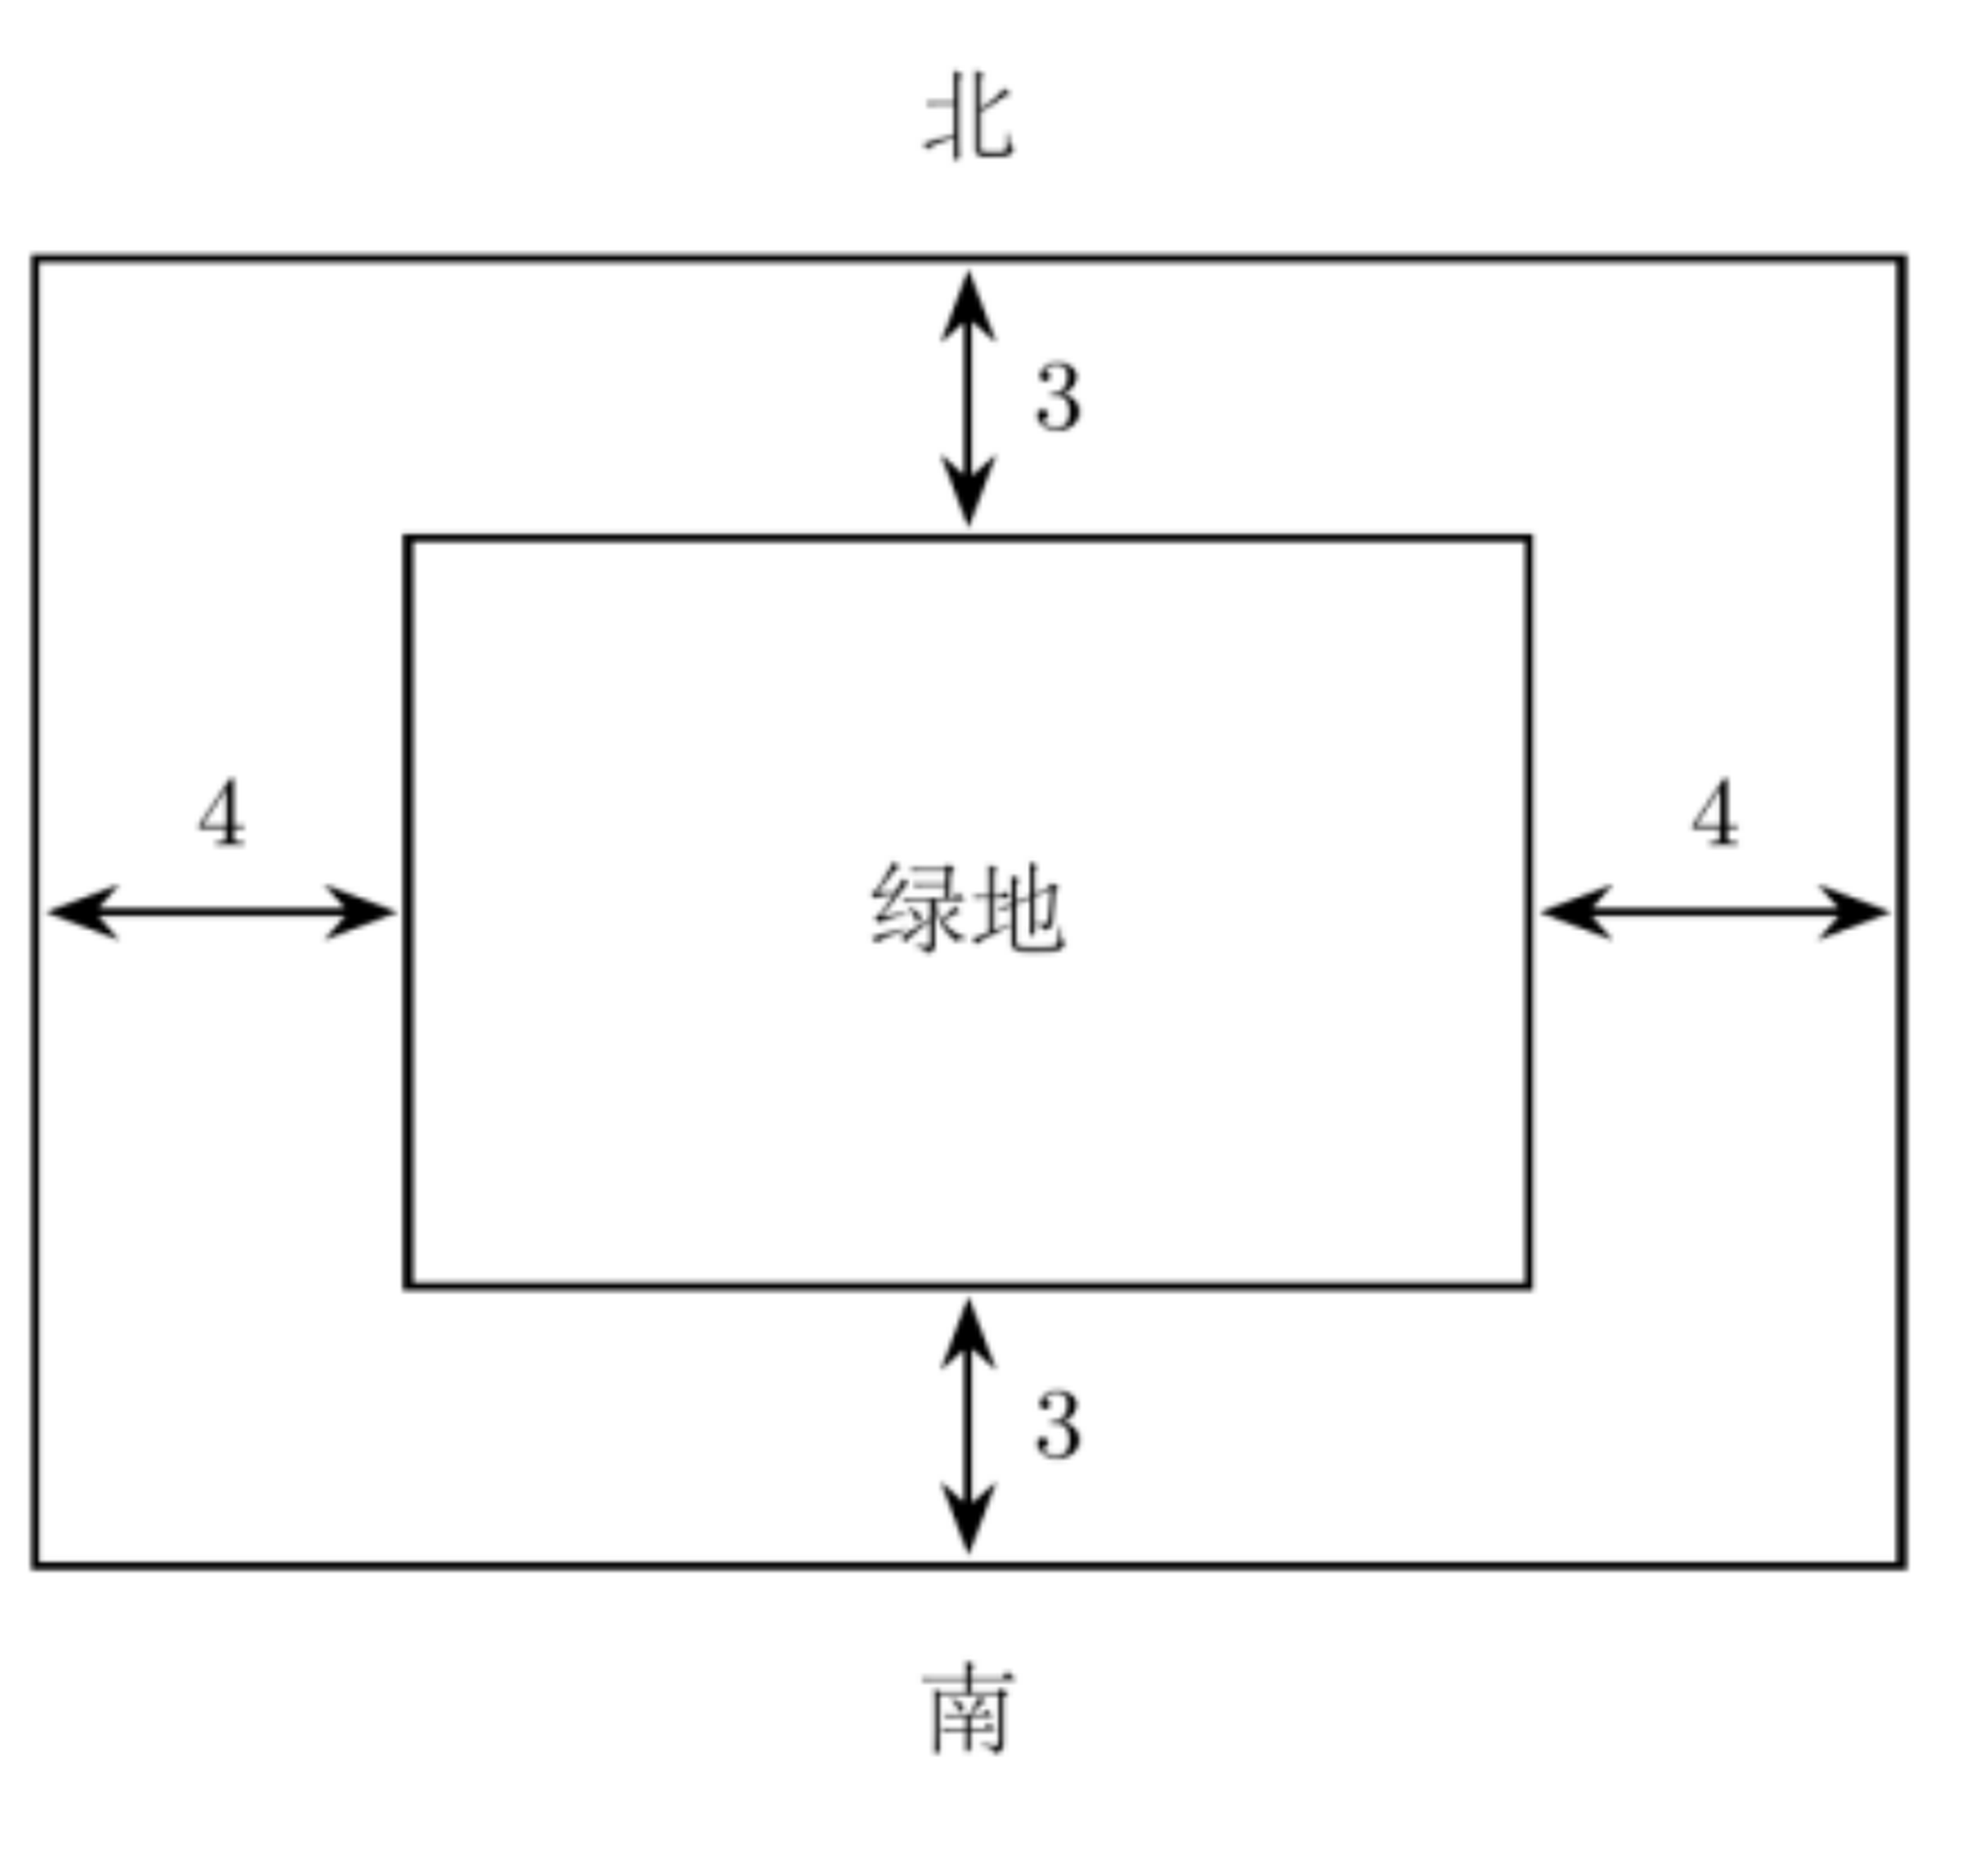
\includegraphics[width=0.32\textwidth]{figures/gao129_q19.png}
\end{center}

(1) 将 $S$ 表示为 $x$ 的函数；

(2) 试确定绿地东西方向的边长和南北方向的边长，使人行道的占地面积最小，并求出人行道的占地最小面积（结果精确到 0.1 米）

\ifanswer
\solbegin
\step{(1) 绿地南北方向的边长为 $\dfrac{1000}{x}$ 米，$x>0$.}
\step{外矩形东西、南北方向的边长分别为 $x+8$ 米、$\dfrac{1000}{x}+6$ 米.}
\step{因此 $S=(x+8)\left(\dfrac{1000}{x}+6\right)-1000=6x+\dfrac{8000}{x}+48, x>0$.}
\step{(2) 因为 $x>0,S=6x+\dfrac{8000}{x}+48\geqslant2\sqrt{6x\cdot\dfrac{8000}{x}}+48=48+80\sqrt{30}$.}
\step{等号当且仅当 $6x=\dfrac{8000}{x}$，即 $x=\dfrac{20\sqrt{30}}{3}\approx36.5$ 时成立，}
\step{此时绿地南北方向的边长为 $\dfrac{1000}{x}=\dfrac{1000}{\dfrac{20\sqrt{30}}{3}}=5\sqrt{30}\approx27.4$（米），}
\step{所以绿地东西方向、南北方向的边长分别约为 36.5 米、27.4 米时，}
\step{人行道的占地面积最小，最小面积为 $S_{min}=48+80\sqrt{30}\approx486.2$ 平方米.}
\solend
\fi

\item 已知集合 $A=\{x\mid x^2-3x+2=0\},B=\{x\mid x^2-ax+a-1=0\}$，

$C=\{x\mid x^2+2(m+1)x+m^2-5=0\}$.

(1) 若 $A=B$，求实数 $a$ 的值；

(2) 若 $B=\{1\}$，求实数 $a$ 的值；

(3) 若 $A\cap C=C$，求实数 $m$ 的取值范围.

\ifanswer
\solbegin
\step{(1) $A=\{1,2\}$，且 $x^2-ax+a-1=(x-1)(x-a+1)$，所以 $B=\{1,a-1\}$，}
\step{因此 $A=B\Leftrightarrow a-1=2\Leftrightarrow a=3$.}
\step{(2) $B=\{1\}$ 表示原方程只有一个不同的实数根，}
\step{得 $a-1=1$，即 $a=2$.}
\step{当 $a=2$ 时，原方程为 $(x-1)^2=0$，符合题意.}
\step{(3) $A\cap C=C\Leftrightarrow C\subseteq\{1,2\}$，}
\step{方程的判别式为 $\Delta=[2(m+1)]^2-4(m^2-5)=8(m+3)$.}
\step{当 $m<-3$ 时，$\Delta<0, C=\varnothing$，满足条件.}
\step{当 $m=-3$ 时，原方程为 $(x-2)^2=0, C=\{2\}$，满足条件.}
\step{当 $m>-3$ 时，方程有两个不同的实数根，必须有 $C=\{1,2\}$，}
\step{由韦达定理，$\begin{cases}-2(m+1)=1+2=3\\m^2-5=1\cdot2=2\end{cases}$，}
\step{第一式得 $m=-\dfrac52$，但此时 $m^2-5=\dfrac54\neq2$，不合题意.}
\step{因此 $m$ 的取值范围为 $(-\infty,-3]$.}
\solend
\fi

\item 设函数 $f(x)=ax^2+(1-a)x+a-2(a\in\R)$.

(1) 若关于 $x$ 的不等式 $f(x)\leqslant0$ 的解集为 $\left[0,\dfrac12\right]$，求实数 $a$ 的值；

(2) 若不等式 $f(x)\geqslant-2$ 对于实数 $a\in[-1,1]$ 时恒成立，求 $x$ 的取值范围；

(3) 解关于 $x$ 的不等式：$f(x)<a-1$.

\ifanswer
\solbegin
\step{(1) 由题意得 $0,\dfrac12$ 是方程 $ax^2+(1-a)x+a-2=0$ 的两个根，}
\step{则 $\begin{cases}0+\dfrac12=-\dfrac{1-a}{a}\\0\times\dfrac12=\dfrac{a-2}{a}\end{cases}\Rightarrow a=2$；}
\step{(2) $ax^2+(1-a)x+a-2\geqslant-2\Rightarrow a(x^2-x+1)+x\geqslant0$ 对 $a\in[-1,1]$ 恒成立，}
\step{则 $\begin{cases}-(x^2-x+1)+x\geqslant0\\(x^2-x+1)+x\geqslant0\end{cases}\Rightarrow\begin{cases}x=1\\x\in\R\end{cases}\Rightarrow x=1$，则 $x$ 的取值范围为 $\{1\}$；}
\step{(3) $f(x)<a-1$ 等价于 $ax^2+(1-a)x-1<0$，}
\step{当 $a=0$ 时，不等式可化为 $x<1$，解集为 $\{x\mid x<1\}$，}
\step{当 $a>0$ 时，不等式可化为 $(ax+1)(x-1)<0$，解集为 $\{x\mid -\dfrac1a<x<1\}$；}
\step{当 $a<0$ 时，不等式化为 $(ax+1)(x-1)<0$，}
\step{①当 $a=-1$ 时，$-\dfrac1a=1$，不等式的解集为 $\{x\mid x\neq1\}$；}
\step{②当 $-1<a<0$ 时，$-\dfrac1a>1$，不等式的解集为 $\{x\mid x<1$ 或 $x>-\dfrac1a\}$；}
\step{③当 $a<-1$ 时，$-\dfrac1a<1$，不等式的解集为 $\{x\mid x<-\dfrac1a$ 或 $x>1\}$；}
\step{综上，当 $a<-1$ 时，解集为 $\{x\mid x<-\dfrac1a$ 或 $x>1\}$；}
\step{当 $a=-1$ 时，解集为 $\{x\mid x\neq1\}$；}
\step{当 $-1<a<0$ 时，解集为 $\{x\mid x<1$ 或 $x>-\dfrac1a\}$；}
\step{当 $a=0$ 时，解集为 $\{x\mid x<1\}$；}
\step{当 $a>0$ 时，解集为 $\{x\mid -\dfrac1a<x<1\}$.}
\solend
\fi

\end{enumerate}

\end{document}
"
%
% 原始材料：微信公众号"魔都数学加油站"文章，作者破晓，2026-11-12 18:56 发布；
% 连载"27学年高一129"，原文标题"27学年高一129——2026-2027年上海市立达中学高一上期中"；
% 原文链接：https://mp.weixin.qq.com/s/gJhGsOBiWi7gW62u8EWLYA。
% 正文为 8 张 PNG 页（01、02、03、05、06 为 4762x6735，04、07、08 为 2560x3620），
% 题目下印有【解析】或【答案】，为讲评版。题目、解析均据原图转录；
% 卷面粉红色水印"魔都数学加油站"及公众号页脚未录入。全卷仅第 19 题有 1 幅插图。
%
% 卷首标题：原卷印作"2026-2027 年立达中学高一上期中"（公众号标题中的"上海市"
% 卷面标题行没有，本稿照卷面），年份区间按全稿惯例排 en dash；原卷未印副标题，
% 本卷为期中卷、跨集合与常用逻辑用语／不等式／函数三章，按题目内容标为
% "集合与常用逻辑用语、不等式、函数"（与 125、126 同为期中卷，口径相同）：
% 集合与逻辑见 Q3、Q4、Q13、Q20，不等式见 Q5、Q6、Q7、Q9、Q10、Q11、Q12、
% Q14、Q15、Q16、Q17、Q18、Q21，函数（含二次函数、基本不等式应用）见 Q8、Q19、Q21。
%
% 与原卷的排版差异：
%   ① 原文从第 3 题起，填空题编号为 3—12、选择题为 13—16、解答题为 17—21，本稿保留原题号；
%   ② 原卷每题下直接印【解析】／【答案】，本稿按全稿惯例置于答案版；第 3、5 题只印
%      【答案】，另提 \ans{}；第 13—16 题答案均在【解析】末句"故选 …"，题干括号内留空、
%      不另提 \ans{}；四道选择题括号内原卷均未印答案；
%   ③ 原卷未印副标题，本稿按"知识模块"口径补出（见上"卷首标题"）；
%   ④ 原卷填空横线按全稿惯例排为 \blankline[4.4em]；选择题括号排 \mbox{（\quad）}、
%      选项段前按惯例加 \keepwithprev；解答题不留作答区（原卷为讲评版，与 109—128 同）；
%   ⑤ 原卷数集排斜体 $R$，按全稿惯例改 \R；绝对值排 \lvert…\rvert，集合描述竖线排 \mid；
%      不等号按全稿惯例排 \leqslant／\geqslant；子题标号原卷一律用半角括号 (1)(2)(3)，本稿照录；
%   ⑥ 原卷第 19 题插图浮排在 Q18 解析右侧、"19."题干之上，本稿按体例就近置于 Q19
%      题干"如图所示"之后（居中 \includegraphics），图取原卷截图去水印；题前按惯例加
%      \needvspace{7cm} 守卫（照 高一120／127 成例），保证"题干 + 图"整块不被页边界切开；
%   ⑦ 原卷 Q8 解析续头印在第 2 页页首、Q17 解析续头印在第 5 页页首、Q19 题干续在第 6 页、
%      Q20 解析跨 6—7 页、Q21 解析续头印在第 8 页页首，本稿按题合并连续排版；
%      末页第 8 页为 Q21 解析的续尾，按实际印刷行单列（照 高一127 第 09 页续尾成例）。
%
% 判别式字形：第 8 题解析 $\Delta=m^2+4m>0$、第 10 题解析 $\Delta=k^2+6k=k(k+6)<0$、
%   第 20 题 (3) 解析 $\Delta=[2(m+1)]^2-4(m^2-5)=8(m+3)$ 三处原卷均排 $\Delta$
%   （等腰、高；回原图逐处放大核对、三处字形一致），照录 \Delta；全卷未出现 \triangle
%   （等边、扁）。
%
% 子集符号：第 13 题 ② $\{0,1,2\}\subseteq\{2,1,0\}$、③ $\varnothing\subseteq\{0,1,2\}$，
%   第 17 题 (2)② $B\subseteq A$、$B\subseteq(3,+\infty)$，第 20 题 (3) $C\subseteq\{1,2\}$
%   均印带下划线，照录 \subseteq；全卷未出现单线 \subset（回原图放大逐处确认）。
%
% 原卷存疑照录：
%   第 15 题解析"即 $m=4$，$n=3$ 时取等号"与题干 $\dfrac1m+n=1$、等号条件
%     $mn=\dfrac9{mn}$ 均不一致（按题应为 $n=\dfrac34$），照录、未统一；
%   第 18 题 (1) 题干"设 $M=2x^2+3x-1,N=7x-3$ 比较 $M$ 与 $N$ 两个数的大小"
%     两式间用半角逗号、且"$N=7x-3$"后无标点直接接"比较"，照录；
%   第 11 题解析"$1-x+2x-1=-(3x-2), 4x=2, x=\dfrac12$"、第 14 题解析
%     "$a=2, b=1, c=4, d=0$"、第 19 题解析"$6x+\dfrac{8000}{x}+48, x>0$"、
%     第 20 题解析"$\Delta<0, C=\varnothing$"与"$(x-2)^2=0, C=\{2\}$"、
%     第 12 题解析"$(x+y)^2=3+t\geqslant0,(x-y)^2=3-3t\geqslant0$"等处数学式内
%     用半角逗号，照录；
%   第 19 题题干"如图所示（图中单位：米）设绿地东西方向的边长为 $x$"在右括号后
%     无标点直接续"设"，照录；
%   第 21 题 (3) 解析先按 $a>0$、$a=0$、$a<0$ 分述解集，又在"综上"处重列全部
%     五类（含已给出的 $a>0$、$a=0$），照录；
%   第 21 题 (2) 题干与解析均作 $f(x)\geqslant-2$（与 $a(x^2-x+1)+x\geqslant0$ 相符），
%     照录，勿误读为 $f(x)\geqslant2$。
%
% 行数复核：逐题数 \step 条数，合计 93 条（Q3：0；Q4：2；Q5：0；Q6：3；Q7：3；
% Q8：2；Q9：4；Q10：3；Q11：5；Q12：5；Q13：1；Q14：3；Q15：3；Q16：7；
% Q17：7；Q18：8；Q19：8；Q20：13；Q21：16），与原卷印刷行逐题相等
% （cases 块作一个印刷行计）。第 3、5 题只印【答案】，提 \ans{}，不计入 \step 账；
% 四道选择题答案均在解析末句，括号内留空、不另提 \ans{}。
%
\documentclass[a4paper,11pt]{article}
\usepackage{common}

\begin{document}

\examtitlest[3]{2026--2027 年立达中学高一上期中}{集合与常用逻辑用语、不等式、函数}

\bigsec{一、填空题}

\begin{enumerate}
\setcounter{enumi}{2}

\item 若 $A=\{x\mid -3<x\leqslant2\},B=\{x\mid 1<x\leqslant3\}$，则 $A\cup B=$\blankline[4.4em].

\ifanswer
\ans{$(-3,3]$}
\fi

\item 若 $A$ 是 $B$ 的必要非充分条件，$B$ 是 $C$ 的充要条件，$C$ 是 $D$ 的必要非充分条件，则 $D$ 是 $A$ 的\blankline[4.4em]条件.

\ifanswer
\solbegin
\step{$D\Rightarrow C\Leftrightarrow B\Rightarrow A$，且 $A\nRightarrow B$，因此 $D\Rightarrow A$ 且 $A\nRightarrow D$，}
\step{故 $D$ 是 $A$ 的充分非必要条件.}
\solend
\fi

\item 不等式 $\dfrac1x<1$ 的解集为\blankline[4.4em].

\ifanswer
\ans{$(-\infty,0)\cup(1,+\infty)$}
\fi

\item 已知正实数 $x$、$y$ 满足 $2x+y=2$，则 $xy$ 的最大值为\blankline[4.4em].

\ifanswer
\solbegin
\step{因为 $x>0$，$y>0$，所以 $2x+y\geqslant2\sqrt{2xy}$（当且仅当 $2x=y$ 时，取等号），}
\step{又因为 $2x+y=2$，所以 $2\geqslant2\sqrt{2xy}$（当且仅当 $2x=y$ 时，取等号），}
\step{即 $xy\leqslant\dfrac12$，则 $xy$ 的最大值为 $\dfrac12$.}
\solend
\fi

\item 已知 $x\in\R$，函数 $y=\lvert x+2\rvert+\lvert x-3\rvert$ 的最小值为\blankline[4.4em].

\ifanswer
\solbegin
\step{由 $\lvert x+2\rvert+\lvert x-3\rvert\geqslant\lvert(x+2)-(x-3)\rvert=5$，}
\step{当且仅当 $(x+2)(x-3)\leqslant0$，即 $-2\leqslant x\leqslant3$ 时，上式取等号，}
\step{则函数 $y=\lvert x+2\rvert+\lvert x-3\rvert$ 的最小值是 5.}
\solend
\fi

\item 已知实系数一元二次方程 $x^2+mx-m=0$ 的两根分别为 $x_1,x_2$，且 $\lvert x_1-x_2\rvert=\sqrt{21}$，实数 $m$ 的值为\blankline[4.4em].

\ifanswer
\solbegin
\step{由题意得 $\Delta=m^2+4m>0$，解得 $m>0$ 或 $m<-4,x_1+x_2=-m,x_1x_2=-m$，}
\step{则 $\lvert x_1-x_2\rvert=\sqrt{(x_1+x_2)^2-4x_1x_2}=\sqrt{m^2+4m}=\sqrt{21}$，解得 $m=-7$ 或 $3$.}
\solend
\fi

\item 已知不等式 $ax^2-5x+b>0$ 的解集是 $\{x\mid -3<x<-2\}$，则不等式 $bx^2-5x+a>0$ 的解集是\blankline[4.4em].

\ifanswer
\solbegin
\step{$ax^2-5x+b=a(x+3)(x+2)$，比较系数得 $5a=-5,b=6a$，}
\step{即 $a=-1,b=-6$.}
\step{$bx^2-5x+a>0\Leftrightarrow(3x+1)(2x+1)<0\Leftrightarrow-\dfrac12<x<-\dfrac13$，}
\step{故解集为 $\left\{x\mid -\dfrac12<x<-\dfrac13\right\}$.}
\solend
\fi

\item 不等式 $4kx^2+kx-\dfrac38<0$ 对于一切实数 $x$ 都成立，则实数 $k$ 的取值范围是\blankline[4.4em].

\ifanswer
\solbegin
\step{$k=0$ 时，不等式恒成立；}
\step{$k\neq0$ 时，须 $4k<0$ 且 $\Delta=k^2+6k=k(k+6)<0$，解得 $-6<k<0$.}
\step{因此 $k\in(-6,0]$.}
\solend
\fi

\item 设 $x\in\R$，方程 $\lvert 1-x\rvert+\lvert 2x-1\rvert=\lvert 3x-2\rvert$ 的解集为\blankline[4.4em].

\ifanswer
\solbegin
\step{当 $x\leqslant\dfrac12$ 时，方程化为 $1-x-(2x-1)=-(3x-2)$，$2-3x=-3x+2$，恒成立，}
\step{当 $\dfrac12<x\leqslant\dfrac23$ 时，方程化为 $1-x+2x-1=-(3x-2), 4x=2, x=\dfrac12$，不合题意，}
\step{当 $\dfrac23<x\leqslant1$ 时，方程化为 $1-x+2x-1=3x-2$，$2x=2$，解得 $x=1$，}
\step{当 $x>1$ 时，方程化为 $-(1-x)+2x-1=3x-2$，$3x-2=3x-2$，恒成立，}
\step{综上所述，$\lvert 1-x\rvert+\lvert 2x-1\rvert=\lvert 3x-2\rvert$ 的解集为 $\left(-\infty,\dfrac12\right]\cup[1,+\infty)$.}
\solend
\fi

\item 已知非零实数 $x,y$ 满足 $x^2+xy+y^2=3$，则 $x^2-xy+y^2$ 的取值范围是\blankline[4.4em].

\ifanswer
\solbegin
\step{令 $t=xy\neq0$，由 $(x+y)^2=3+t\geqslant0,(x-y)^2=3-3t\geqslant0$，}
\step{得 $t\in[-3,0)\cup(0,1]$.}
\step{对上述任意 $t$，联立 $x+y=\sqrt{3+t},x-y=\sqrt{3-3t}$，所得 $x,y$ 满足原条件，}
\step{因此上述 $t$ 均可取到.}
\step{于是 $x^2-xy+y^2=3-2t$ 的取值范围为 $[1,3)\cup(3,9]$.}
\solend
\fi

\end{enumerate}

\bigsec{二、选择题}

\begin{enumerate}
\setcounter{enumi}{12}

\item 下列各式中，正确的个数是\mbox{（\quad）}

① $\{0\}\in\{0,1,2\}$；② $\{0,1,2\}\subseteq\{2,1,0\}$；③ $\varnothing\subseteq\{0,1,2\}$；④ $\varnothing=\{0\}$；⑤ $\{0,1\}=\{(0,1)\}$；

⑥ $0=\{0\}$.

\keepwithprev
A. $1$\qquad\qquad B. $2$\qquad\qquad C. $3$\qquad\qquad D. $4$

\ifanswer
\solbegin
\step{①不正确，②正确，③正确，④不正确，⑤不正确，⑥不正确. 故选 $B$.}
\solend
\fi

\item 下列四个命题中，为真命题的是\mbox{（\quad）}

\keepwithprev
A. 若 $a>b$，则 $ac^2>bc^2$\qquad\qquad B. 若 $a>b,c>d$，则 $a-c>b-d$

C. 若 $ac^2>bc^2$，则 $a>b$\qquad\qquad D. 若 $a>b$，则 $\dfrac1a<\dfrac1b$

\ifanswer
\solbegin
\step{C 中，$(a-b)c^2>0$，必有 $c^2>0$ 且 $a-b>0$，即 $a>b$.}
\step{A 取 $c=0$；B 取 $a=2, b=1, c=4, d=0$；D 取 $a=1, b=-1$，均不成立.}
\step{故选 $C$.}
\solend
\fi

\item 已知 $m$、$n\in(0,+\infty)$，$\dfrac1m+n=1$，则 $m+\dfrac9n$ 的最小值为\mbox{（\quad）}

\keepwithprev
A. $13$\qquad\qquad B. $16$\qquad\qquad C. $3$\qquad\qquad D. $6$

\ifanswer
\solbegin
\step{因为 $m$、$n\in(0,+\infty)$，$\dfrac1m+n=1$，}
\step{所以 $m+\dfrac9n=(m+\dfrac9n)(\dfrac1m+n)=10+mn+\dfrac9{mn}\geqslant10+2\sqrt{mn\cdot\dfrac9{mn}}=16$，}
\step{当且仅当 $mn=\dfrac9{mn}$，即 $m=4$，$n=3$ 时取等号. 故选 $B$.}
\solend
\fi

\item 下列不等式：① $\left\lvert x+\dfrac1x\right\rvert\geqslant2$；② $x^2+2x+1>0$；③ $\lvert x\rvert+\lvert x-1\rvert\geqslant1$；④ $\dfrac{x}{x^2+x+1}<1$；

解集为 $\R$ 的不等式的个数是\mbox{（\quad）}

\keepwithprev
A. $0$\qquad\qquad B. $1$\qquad\qquad C. $2$\qquad\qquad D. $3$

\ifanswer
\solbegin
\step{对于①，当 $x=0$ 时，$\dfrac1x$ 无意义，故 $\left\lvert x+\dfrac1x\right\rvert\geqslant2$ 的解集不是 $\R$，错误；}
\step{对于②，$x^2+2x+1=(x+1)^2\geqslant0$，当 $x=-1$ 取到等号，解集不是 $\R$，故错误；}
\step{对于③，$\lvert x\rvert+\lvert x-1\rvert\geqslant\lvert x-(x-1)\rvert=1$，当 $x(x-1)\leqslant0$ 时取等号，解集为 $\R$，}
\step{故正确；}
\step{对于④，由于 $x^2+x+1>0$ 恒成立，}
\step{故 $\dfrac{x}{x^2+x+1}<1$ 等价于 $x<x^2+x+1\Rightarrow x^2+1>0$ 恒成立，故解集为 $\R$，正确，}
\step{故正确的有③④，故选 $C$.}
\solend
\fi

\end{enumerate}

\bigsec{三、解答题}

\begin{enumerate}
\setcounter{enumi}{16}

\item (1) 解不等式组 $\begin{cases}\dfrac{x+3}{x+1}\leqslant2\\\lvert 2x-3\rvert\leqslant2\end{cases}$.

(2) 已知集合 $A=\{x\mid -x+3<0\},B=\{x\mid a\leqslant x\leqslant a+3\}$.

①当 $a=2$，求集合 $A\cap B$；

②若 $A\cup B=A$，求实数 $a$ 的取值范围.

\ifanswer
\solbegin
\step{(1) 由 $\begin{cases}\dfrac{x+3}{x+1}\leqslant2\\\lvert 2x-3\rvert\leqslant2\end{cases}$ 得 $\begin{cases}\dfrac{x+3-2x-2}{x+1}\leqslant0\\-2\leqslant2x-3\leqslant2\end{cases}$，即 $\begin{cases}\dfrac{-x+1}{x+1}\leqslant0\\1\leqslant2x\leqslant5\end{cases}$，则 $\begin{cases}\dfrac{x-1}{x+1}\geqslant0\\\dfrac12\leqslant x\leqslant\dfrac52\end{cases}$，}
\step{解得 $1\leqslant x\leqslant\dfrac52$，即原不等式组的解集为 $\left[1,\dfrac52\right]$.}
\step{(2) $-x+3<0\Leftrightarrow x>3$，所以 $A=(3,+\infty)$.}
\step{①当 $a=2$ 时，$B=[2,5], A\cap B=(3,+\infty)\cap[2,5]=(3,5]$.}
\step{②$A\cup B=A\Leftrightarrow B\subseteq A$.}
\step{因为 $B=[a,a+3]$，且左端点 $a\in B$，所以 $B\subseteq(3,+\infty)\Leftrightarrow a>3$，}
\step{实数 $a$ 的取值范围为 $(3,+\infty)$.}
\solend
\fi

\item (1) 设 $M=2x^2+3x-1,N=7x-3$ 比较 $M$ 与 $N$ 两个数的大小.

(2) 解关于 $x$ 的不等式：$x^2-(a+3)x+3a<0$，$a\in\R$.

\ifanswer
\solbegin
\step{(1) $M-N=2x^2+3x-1-(7x-3)=2(x-1)^2$.}
\step{$x=1$ 时，$M-N=0$，即 $M=N$.}
\step{$x\neq1$ 时，$M-N>0$，即 $M>N$.}
\step{(2) 不等式 $x^2-(a+3)x+3a<0$ 可化为 $(x-3)(x-a)<0$，}
\step{不等式对应方程的解为 $a$ 和 3，}
\step{当 $a<3$ 时，不等式 $x^2-(a+3)x+3a<0$ 的解集为 $(a,3)$，}
\step{当 $a=3$ 时，不等式 $x^2-(a+3)x+3a<0$ 的解集为 $\varnothing$，}
\step{当 $a>3$ 时，不等式 $x^2-(a+3)x+3a<0$ 的解集为 $(3,a)$.}
\solend
\fi

% 第 19 题是"题干 + 图"约 7cm 的一整块，答案版实测断点落在题干之后（图被推到次页页首），
% 照 高一120／127 成例在题前先量一次页高，不够就把"题干 + 图"整块一起挪到次页。
\needvspace{7cm}
\item 某新建居民小区欲建一面积为 1000 平方米的矩形绿地，在绿地四周铺设人行道，设计要求绿地南北两侧人行道宽 3 米，东西两侧人行道宽 4 米，如图所示（图中单位：米）设绿地东西方向的边长为 $x$，人行道的占地面积为 $S$.

\begin{center}
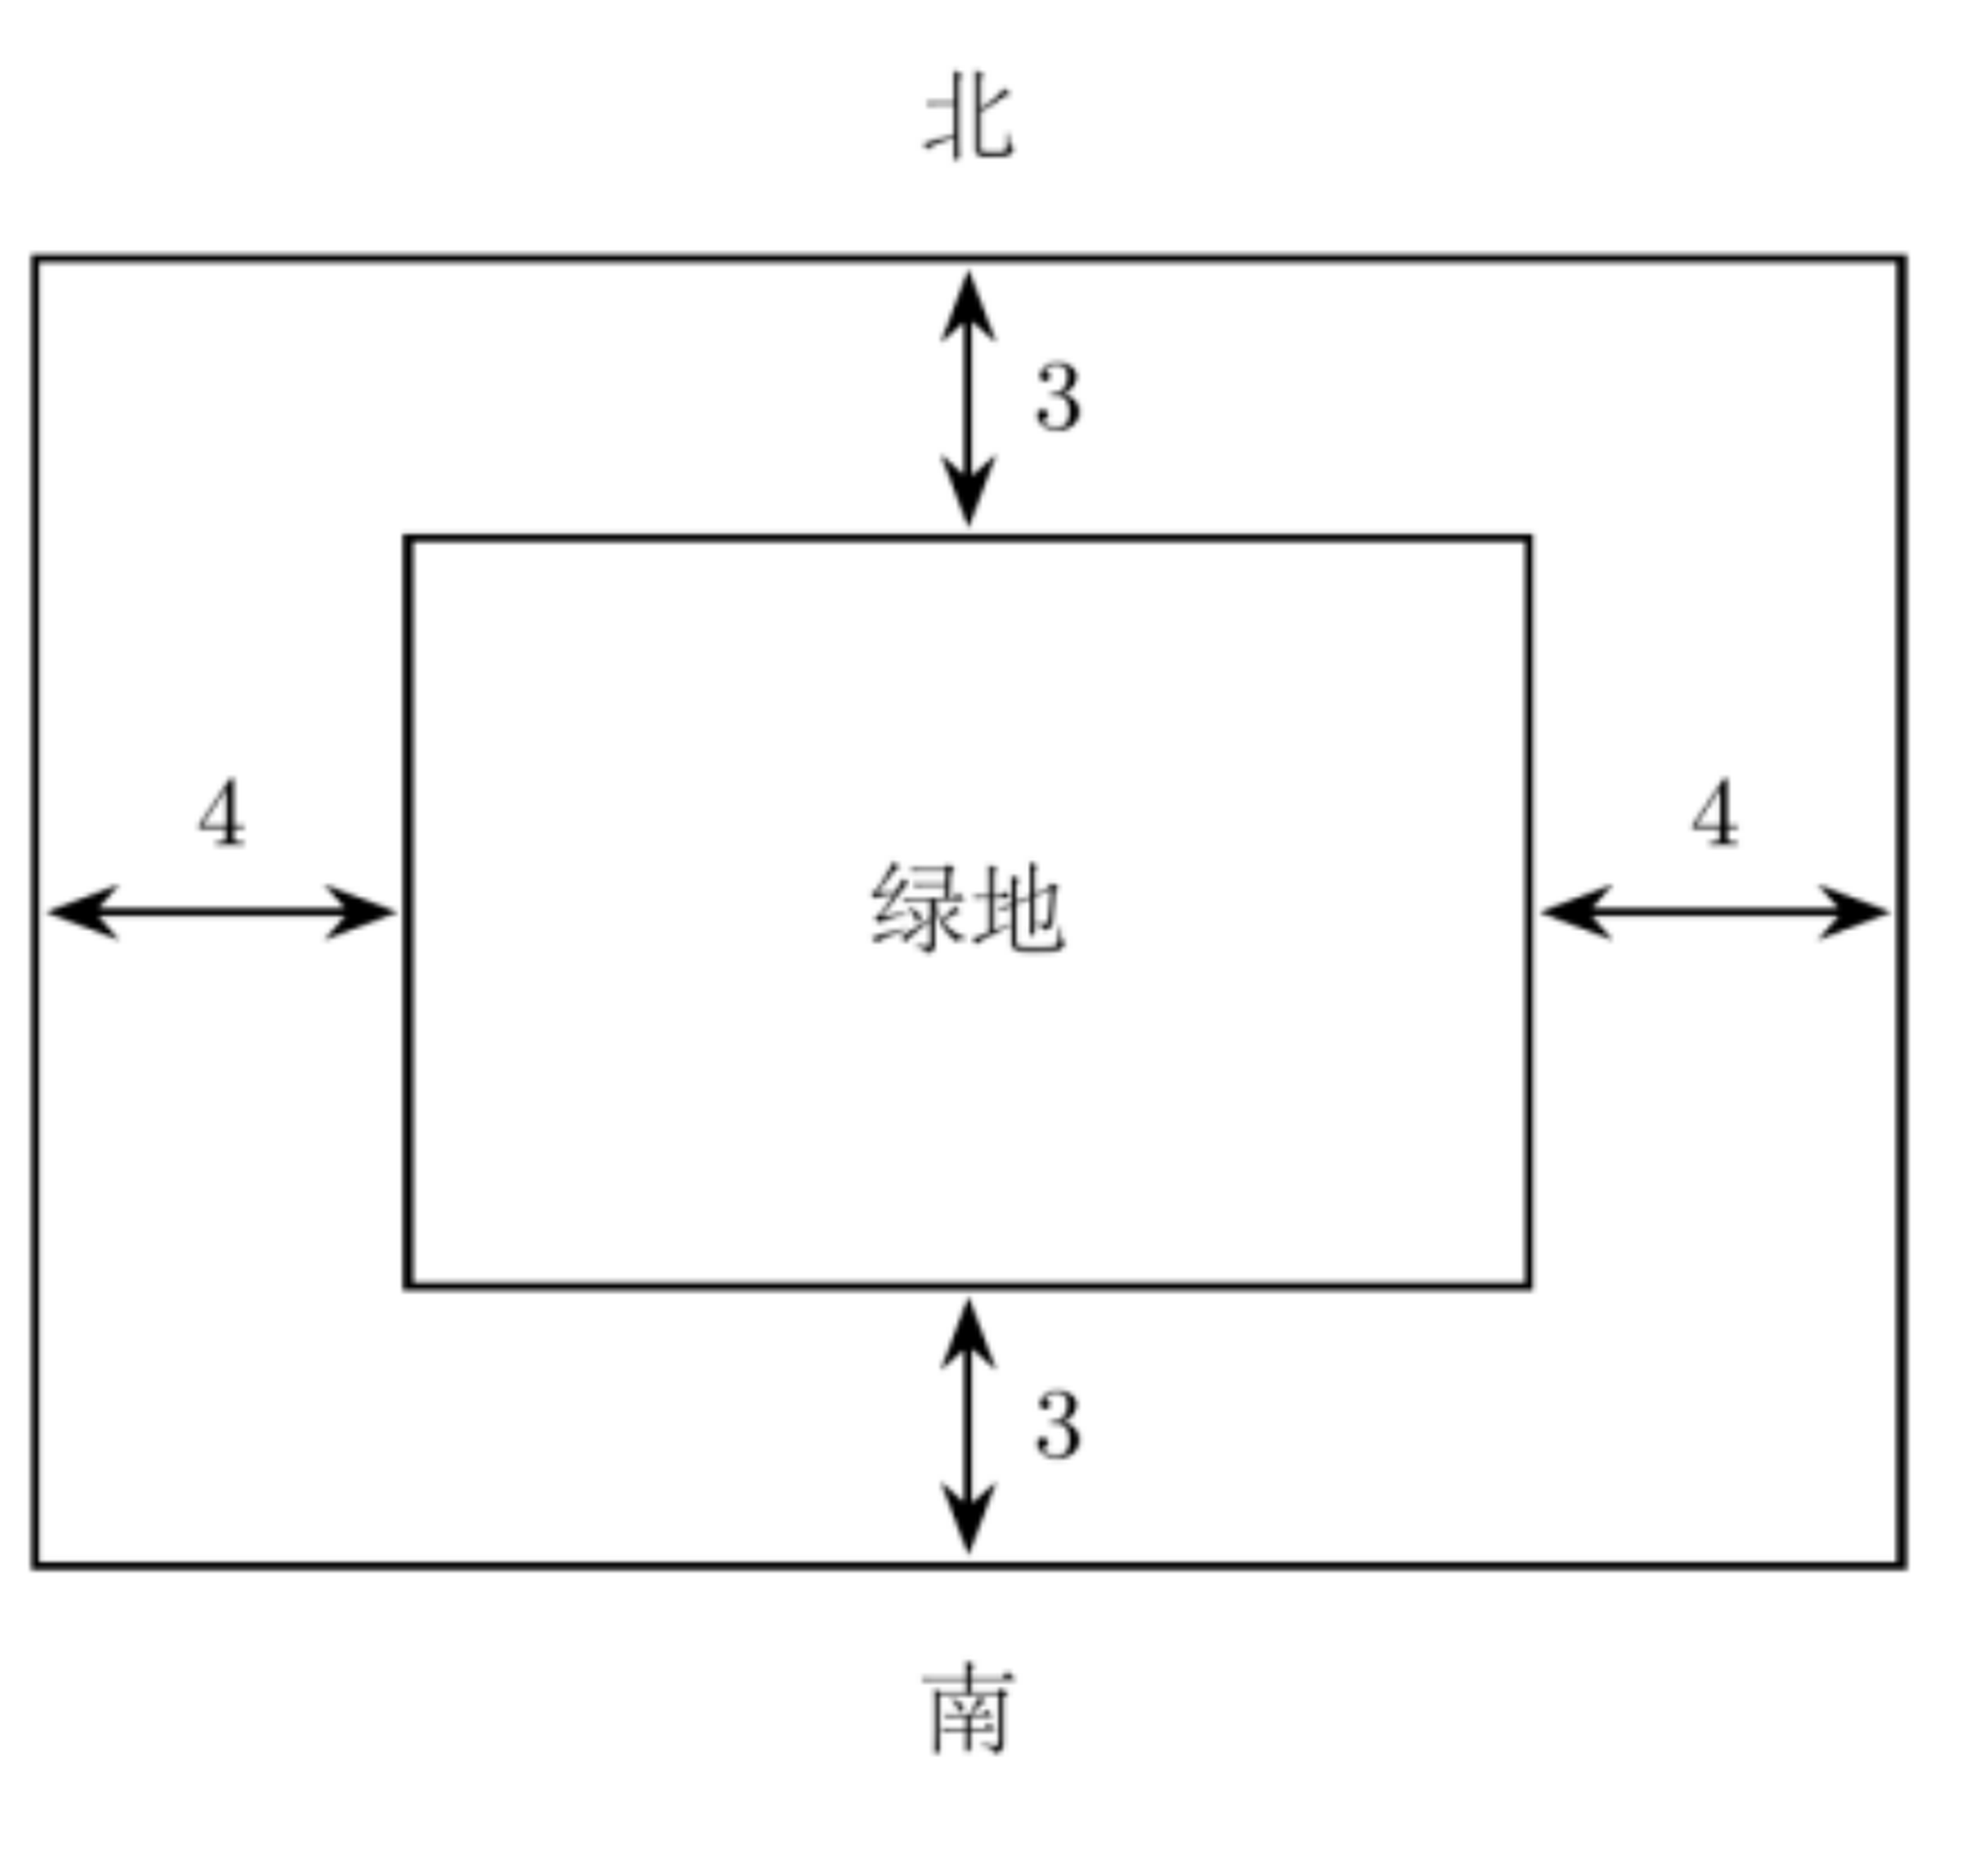
\includegraphics[width=0.32\textwidth]{figures/gao129_q19.png}
\end{center}

(1) 将 $S$ 表示为 $x$ 的函数；

(2) 试确定绿地东西方向的边长和南北方向的边长，使人行道的占地面积最小，并求出人行道的占地最小面积（结果精确到 0.1 米）

\ifanswer
\solbegin
\step{(1) 绿地南北方向的边长为 $\dfrac{1000}{x}$ 米，$x>0$.}
\step{外矩形东西、南北方向的边长分别为 $x+8$ 米、$\dfrac{1000}{x}+6$ 米.}
\step{因此 $S=(x+8)\left(\dfrac{1000}{x}+6\right)-1000=6x+\dfrac{8000}{x}+48, x>0$.}
\step{(2) 因为 $x>0,S=6x+\dfrac{8000}{x}+48\geqslant2\sqrt{6x\cdot\dfrac{8000}{x}}+48=48+80\sqrt{30}$.}
\step{等号当且仅当 $6x=\dfrac{8000}{x}$，即 $x=\dfrac{20\sqrt{30}}{3}\approx36.5$ 时成立，}
\step{此时绿地南北方向的边长为 $\dfrac{1000}{x}=\dfrac{1000}{\dfrac{20\sqrt{30}}{3}}=5\sqrt{30}\approx27.4$（米），}
\step{所以绿地东西方向、南北方向的边长分别约为 36.5 米、27.4 米时，}
\step{人行道的占地面积最小，最小面积为 $S_{min}=48+80\sqrt{30}\approx486.2$ 平方米.}
\solend
\fi

\item 已知集合 $A=\{x\mid x^2-3x+2=0\},B=\{x\mid x^2-ax+a-1=0\}$，

$C=\{x\mid x^2+2(m+1)x+m^2-5=0\}$.

(1) 若 $A=B$，求实数 $a$ 的值；

(2) 若 $B=\{1\}$，求实数 $a$ 的值；

(3) 若 $A\cap C=C$，求实数 $m$ 的取值范围.

\ifanswer
\solbegin
\step{(1) $A=\{1,2\}$，且 $x^2-ax+a-1=(x-1)(x-a+1)$，所以 $B=\{1,a-1\}$，}
\step{因此 $A=B\Leftrightarrow a-1=2\Leftrightarrow a=3$.}
\step{(2) $B=\{1\}$ 表示原方程只有一个不同的实数根，}
\step{得 $a-1=1$，即 $a=2$.}
\step{当 $a=2$ 时，原方程为 $(x-1)^2=0$，符合题意.}
\step{(3) $A\cap C=C\Leftrightarrow C\subseteq\{1,2\}$，}
\step{方程的判别式为 $\Delta=[2(m+1)]^2-4(m^2-5)=8(m+3)$.}
\step{当 $m<-3$ 时，$\Delta<0, C=\varnothing$，满足条件.}
\step{当 $m=-3$ 时，原方程为 $(x-2)^2=0, C=\{2\}$，满足条件.}
\step{当 $m>-3$ 时，方程有两个不同的实数根，必须有 $C=\{1,2\}$，}
\step{由韦达定理，$\begin{cases}-2(m+1)=1+2=3\\m^2-5=1\cdot2=2\end{cases}$，}
\step{第一式得 $m=-\dfrac52$，但此时 $m^2-5=\dfrac54\neq2$，不合题意.}
\step{因此 $m$ 的取值范围为 $(-\infty,-3]$.}
\solend
\fi

\item 设函数 $f(x)=ax^2+(1-a)x+a-2(a\in\R)$.

(1) 若关于 $x$ 的不等式 $f(x)\leqslant0$ 的解集为 $\left[0,\dfrac12\right]$，求实数 $a$ 的值；

(2) 若不等式 $f(x)\geqslant-2$ 对于实数 $a\in[-1,1]$ 时恒成立，求 $x$ 的取值范围；

(3) 解关于 $x$ 的不等式：$f(x)<a-1$.

\ifanswer
\solbegin
\step{(1) 由题意得 $0,\dfrac12$ 是方程 $ax^2+(1-a)x+a-2=0$ 的两个根，}
\step{则 $\begin{cases}0+\dfrac12=-\dfrac{1-a}{a}\\0\times\dfrac12=\dfrac{a-2}{a}\end{cases}\Rightarrow a=2$；}
\step{(2) $ax^2+(1-a)x+a-2\geqslant-2\Rightarrow a(x^2-x+1)+x\geqslant0$ 对 $a\in[-1,1]$ 恒成立，}
\step{则 $\begin{cases}-(x^2-x+1)+x\geqslant0\\(x^2-x+1)+x\geqslant0\end{cases}\Rightarrow\begin{cases}x=1\\x\in\R\end{cases}\Rightarrow x=1$，则 $x$ 的取值范围为 $\{1\}$；}
\step{(3) $f(x)<a-1$ 等价于 $ax^2+(1-a)x-1<0$，}
\step{当 $a=0$ 时，不等式可化为 $x<1$，解集为 $\{x\mid x<1\}$，}
\step{当 $a>0$ 时，不等式可化为 $(ax+1)(x-1)<0$，解集为 $\{x\mid -\dfrac1a<x<1\}$；}
\step{当 $a<0$ 时，不等式化为 $(ax+1)(x-1)<0$，}
\step{①当 $a=-1$ 时，$-\dfrac1a=1$，不等式的解集为 $\{x\mid x\neq1\}$；}
\step{②当 $-1<a<0$ 时，$-\dfrac1a>1$，不等式的解集为 $\{x\mid x<1$ 或 $x>-\dfrac1a\}$；}
\step{③当 $a<-1$ 时，$-\dfrac1a<1$，不等式的解集为 $\{x\mid x<-\dfrac1a$ 或 $x>1\}$；}
\step{综上，当 $a<-1$ 时，解集为 $\{x\mid x<-\dfrac1a$ 或 $x>1\}$；}
\step{当 $a=-1$ 时，解集为 $\{x\mid x\neq1\}$；}
\step{当 $-1<a<0$ 时，解集为 $\{x\mid x<1$ 或 $x>-\dfrac1a\}$；}
\step{当 $a=0$ 时，解集为 $\{x\mid x<1\}$；}
\step{当 $a>0$ 时，解集为 $\{x\mid -\dfrac1a<x<1\}$.}
\solend
\fi

\end{enumerate}

\end{document}
"
%
% 原始材料：微信公众号"魔都数学加油站"文章，作者破晓，2026-11-12 18:56 发布；
% 连载"27学年高一129"，原文标题"27学年高一129——2026-2027年上海市立达中学高一上期中"；
% 原文链接：https://mp.weixin.qq.com/s/gJhGsOBiWi7gW62u8EWLYA。
% 正文为 8 张 PNG 页（01、02、03、05、06 为 4762x6735，04、07、08 为 2560x3620），
% 题目下印有【解析】或【答案】，为讲评版。题目、解析均据原图转录；
% 卷面粉红色水印"魔都数学加油站"及公众号页脚未录入。全卷仅第 19 题有 1 幅插图。
%
% 卷首标题：原卷印作"2026-2027 年立达中学高一上期中"（公众号标题中的"上海市"
% 卷面标题行没有，本稿照卷面），年份区间按全稿惯例排 en dash；原卷未印副标题，
% 本卷为期中卷、跨集合与常用逻辑用语／不等式／函数三章，按题目内容标为
% "集合与常用逻辑用语、不等式、函数"（与 125、126 同为期中卷，口径相同）：
% 集合与逻辑见 Q3、Q4、Q13、Q20，不等式见 Q5、Q6、Q7、Q9、Q10、Q11、Q12、
% Q14、Q15、Q16、Q17、Q18、Q21，函数（含二次函数、基本不等式应用）见 Q8、Q19、Q21。
%
% 与原卷的排版差异：
%   ① 原文从第 3 题起，填空题编号为 3—12、选择题为 13—16、解答题为 17—21，本稿保留原题号；
%   ② 原卷每题下直接印【解析】／【答案】，本稿按全稿惯例置于答案版；第 3、5 题只印
%      【答案】，另提 \ans{}；第 13—16 题答案均在【解析】末句"故选 …"，题干括号内留空、
%      不另提 \ans{}；四道选择题括号内原卷均未印答案；
%   ③ 原卷未印副标题，本稿按"知识模块"口径补出（见上"卷首标题"）；
%   ④ 原卷填空横线按全稿惯例排为 \blankline[4.4em]；选择题括号排 \mbox{（\quad）}、
%      选项段前按惯例加 \keepwithprev；解答题不留作答区（原卷为讲评版，与 109—128 同）；
%   ⑤ 原卷数集排斜体 $R$，按全稿惯例改 \R；绝对值排 \lvert…\rvert，集合描述竖线排 \mid；
%      不等号按全稿惯例排 \leqslant／\geqslant；子题标号原卷一律用半角括号 (1)(2)(3)，本稿照录；
%   ⑥ 原卷第 19 题插图浮排在 Q18 解析右侧、"19."题干之上，本稿按体例就近置于 Q19
%      题干"如图所示"之后（居中 \includegraphics），图取原卷截图去水印；题前按惯例加
%      \needvspace{7cm} 守卫（照 高一120／127 成例），保证"题干 + 图"整块不被页边界切开；
%   ⑦ 原卷 Q8 解析续头印在第 2 页页首、Q17 解析续头印在第 5 页页首、Q19 题干续在第 6 页、
%      Q20 解析跨 6—7 页、Q21 解析续头印在第 8 页页首，本稿按题合并连续排版；
%      末页第 8 页为 Q21 解析的续尾，按实际印刷行单列（照 高一127 第 09 页续尾成例）。
%
% 判别式字形：第 8 题解析 $\Delta=m^2+4m>0$、第 10 题解析 $\Delta=k^2+6k=k(k+6)<0$、
%   第 20 题 (3) 解析 $\Delta=[2(m+1)]^2-4(m^2-5)=8(m+3)$ 三处原卷均排 $\Delta$
%   （等腰、高；回原图逐处放大核对、三处字形一致），照录 \Delta；全卷未出现 \triangle
%   （等边、扁）。
%
% 子集符号：第 13 题 ② $\{0,1,2\}\subseteq\{2,1,0\}$、③ $\varnothing\subseteq\{0,1,2\}$，
%   第 17 题 (2)② $B\subseteq A$、$B\subseteq(3,+\infty)$，第 20 题 (3) $C\subseteq\{1,2\}$
%   均印带下划线，照录 \subseteq；全卷未出现单线 \subset（回原图放大逐处确认）。
%
% 原卷存疑照录：
%   第 15 题解析"即 $m=4$，$n=3$ 时取等号"与题干 $\dfrac1m+n=1$、等号条件
%     $mn=\dfrac9{mn}$ 均不一致（按题应为 $n=\dfrac34$），照录、未统一；
%   第 18 题 (1) 题干"设 $M=2x^2+3x-1,N=7x-3$ 比较 $M$ 与 $N$ 两个数的大小"
%     两式间用半角逗号、且"$N=7x-3$"后无标点直接接"比较"，照录；
%   第 11 题解析"$1-x+2x-1=-(3x-2), 4x=2, x=\dfrac12$"、第 14 题解析
%     "$a=2, b=1, c=4, d=0$"、第 19 题解析"$6x+\dfrac{8000}{x}+48, x>0$"、
%     第 20 题解析"$\Delta<0, C=\varnothing$"与"$(x-2)^2=0, C=\{2\}$"、
%     第 12 题解析"$(x+y)^2=3+t\geqslant0,(x-y)^2=3-3t\geqslant0$"等处数学式内
%     用半角逗号，照录；
%   第 19 题题干"如图所示（图中单位：米）设绿地东西方向的边长为 $x$"在右括号后
%     无标点直接续"设"，照录；
%   第 21 题 (3) 解析先按 $a>0$、$a=0$、$a<0$ 分述解集，又在"综上"处重列全部
%     五类（含已给出的 $a>0$、$a=0$），照录；
%   第 21 题 (2) 题干与解析均作 $f(x)\geqslant-2$（与 $a(x^2-x+1)+x\geqslant0$ 相符），
%     照录，勿误读为 $f(x)\geqslant2$。
%
% 行数复核：逐题数 \step 条数，合计 93 条（Q3：0；Q4：2；Q5：0；Q6：3；Q7：3；
% Q8：2；Q9：4；Q10：3；Q11：5；Q12：5；Q13：1；Q14：3；Q15：3；Q16：7；
% Q17：7；Q18：8；Q19：8；Q20：13；Q21：16），与原卷印刷行逐题相等
% （cases 块作一个印刷行计）。第 3、5 题只印【答案】，提 \ans{}，不计入 \step 账；
% 四道选择题答案均在解析末句，括号内留空、不另提 \ans{}。
%
\documentclass[a4paper,11pt]{article}
\usepackage{common}

\begin{document}

\examtitlest[3]{2026--2027 年立达中学高一上期中}{集合与常用逻辑用语、不等式、函数}

\bigsec{一、填空题}

\begin{enumerate}
\setcounter{enumi}{2}

\item 若 $A=\{x\mid -3<x\leqslant2\},B=\{x\mid 1<x\leqslant3\}$，则 $A\cup B=$\blankline[4.4em].

\ifanswer
\ans{$(-3,3]$}
\fi

\item 若 $A$ 是 $B$ 的必要非充分条件，$B$ 是 $C$ 的充要条件，$C$ 是 $D$ 的必要非充分条件，则 $D$ 是 $A$ 的\blankline[4.4em]条件.

\ifanswer
\solbegin
\step{$D\Rightarrow C\Leftrightarrow B\Rightarrow A$，且 $A\nRightarrow B$，因此 $D\Rightarrow A$ 且 $A\nRightarrow D$，}
\step{故 $D$ 是 $A$ 的充分非必要条件.}
\solend
\fi

\item 不等式 $\dfrac1x<1$ 的解集为\blankline[4.4em].

\ifanswer
\ans{$(-\infty,0)\cup(1,+\infty)$}
\fi

\item 已知正实数 $x$、$y$ 满足 $2x+y=2$，则 $xy$ 的最大值为\blankline[4.4em].

\ifanswer
\solbegin
\step{因为 $x>0$，$y>0$，所以 $2x+y\geqslant2\sqrt{2xy}$（当且仅当 $2x=y$ 时，取等号），}
\step{又因为 $2x+y=2$，所以 $2\geqslant2\sqrt{2xy}$（当且仅当 $2x=y$ 时，取等号），}
\step{即 $xy\leqslant\dfrac12$，则 $xy$ 的最大值为 $\dfrac12$.}
\solend
\fi

\item 已知 $x\in\R$，函数 $y=\lvert x+2\rvert+\lvert x-3\rvert$ 的最小值为\blankline[4.4em].

\ifanswer
\solbegin
\step{由 $\lvert x+2\rvert+\lvert x-3\rvert\geqslant\lvert(x+2)-(x-3)\rvert=5$，}
\step{当且仅当 $(x+2)(x-3)\leqslant0$，即 $-2\leqslant x\leqslant3$ 时，上式取等号，}
\step{则函数 $y=\lvert x+2\rvert+\lvert x-3\rvert$ 的最小值是 5.}
\solend
\fi

\item 已知实系数一元二次方程 $x^2+mx-m=0$ 的两根分别为 $x_1,x_2$，且 $\lvert x_1-x_2\rvert=\sqrt{21}$，实数 $m$ 的值为\blankline[4.4em].

\ifanswer
\solbegin
\step{由题意得 $\Delta=m^2+4m>0$，解得 $m>0$ 或 $m<-4,x_1+x_2=-m,x_1x_2=-m$，}
\step{则 $\lvert x_1-x_2\rvert=\sqrt{(x_1+x_2)^2-4x_1x_2}=\sqrt{m^2+4m}=\sqrt{21}$，解得 $m=-7$ 或 $3$.}
\solend
\fi

\item 已知不等式 $ax^2-5x+b>0$ 的解集是 $\{x\mid -3<x<-2\}$，则不等式 $bx^2-5x+a>0$ 的解集是\blankline[4.4em].

\ifanswer
\solbegin
\step{$ax^2-5x+b=a(x+3)(x+2)$，比较系数得 $5a=-5,b=6a$，}
\step{即 $a=-1,b=-6$.}
\step{$bx^2-5x+a>0\Leftrightarrow(3x+1)(2x+1)<0\Leftrightarrow-\dfrac12<x<-\dfrac13$，}
\step{故解集为 $\left\{x\mid -\dfrac12<x<-\dfrac13\right\}$.}
\solend
\fi

\item 不等式 $4kx^2+kx-\dfrac38<0$ 对于一切实数 $x$ 都成立，则实数 $k$ 的取值范围是\blankline[4.4em].

\ifanswer
\solbegin
\step{$k=0$ 时，不等式恒成立；}
\step{$k\neq0$ 时，须 $4k<0$ 且 $\Delta=k^2+6k=k(k+6)<0$，解得 $-6<k<0$.}
\step{因此 $k\in(-6,0]$.}
\solend
\fi

\item 设 $x\in\R$，方程 $\lvert 1-x\rvert+\lvert 2x-1\rvert=\lvert 3x-2\rvert$ 的解集为\blankline[4.4em].

\ifanswer
\solbegin
\step{当 $x\leqslant\dfrac12$ 时，方程化为 $1-x-(2x-1)=-(3x-2)$，$2-3x=-3x+2$，恒成立，}
\step{当 $\dfrac12<x\leqslant\dfrac23$ 时，方程化为 $1-x+2x-1=-(3x-2), 4x=2, x=\dfrac12$，不合题意，}
\step{当 $\dfrac23<x\leqslant1$ 时，方程化为 $1-x+2x-1=3x-2$，$2x=2$，解得 $x=1$，}
\step{当 $x>1$ 时，方程化为 $-(1-x)+2x-1=3x-2$，$3x-2=3x-2$，恒成立，}
\step{综上所述，$\lvert 1-x\rvert+\lvert 2x-1\rvert=\lvert 3x-2\rvert$ 的解集为 $\left(-\infty,\dfrac12\right]\cup[1,+\infty)$.}
\solend
\fi

\item 已知非零实数 $x,y$ 满足 $x^2+xy+y^2=3$，则 $x^2-xy+y^2$ 的取值范围是\blankline[4.4em].

\ifanswer
\solbegin
\step{令 $t=xy\neq0$，由 $(x+y)^2=3+t\geqslant0,(x-y)^2=3-3t\geqslant0$，}
\step{得 $t\in[-3,0)\cup(0,1]$.}
\step{对上述任意 $t$，联立 $x+y=\sqrt{3+t},x-y=\sqrt{3-3t}$，所得 $x,y$ 满足原条件，}
\step{因此上述 $t$ 均可取到.}
\step{于是 $x^2-xy+y^2=3-2t$ 的取值范围为 $[1,3)\cup(3,9]$.}
\solend
\fi

\end{enumerate}

\bigsec{二、选择题}

\begin{enumerate}
\setcounter{enumi}{12}

\item 下列各式中，正确的个数是\mbox{（\quad）}

① $\{0\}\in\{0,1,2\}$；② $\{0,1,2\}\subseteq\{2,1,0\}$；③ $\varnothing\subseteq\{0,1,2\}$；④ $\varnothing=\{0\}$；⑤ $\{0,1\}=\{(0,1)\}$；

⑥ $0=\{0\}$.

\keepwithprev
A. $1$\qquad\qquad B. $2$\qquad\qquad C. $3$\qquad\qquad D. $4$

\ifanswer
\solbegin
\step{①不正确，②正确，③正确，④不正确，⑤不正确，⑥不正确. 故选 $B$.}
\solend
\fi

\item 下列四个命题中，为真命题的是\mbox{（\quad）}

\keepwithprev
A. 若 $a>b$，则 $ac^2>bc^2$\qquad\qquad B. 若 $a>b,c>d$，则 $a-c>b-d$

C. 若 $ac^2>bc^2$，则 $a>b$\qquad\qquad D. 若 $a>b$，则 $\dfrac1a<\dfrac1b$

\ifanswer
\solbegin
\step{C 中，$(a-b)c^2>0$，必有 $c^2>0$ 且 $a-b>0$，即 $a>b$.}
\step{A 取 $c=0$；B 取 $a=2, b=1, c=4, d=0$；D 取 $a=1, b=-1$，均不成立.}
\step{故选 $C$.}
\solend
\fi

\item 已知 $m$、$n\in(0,+\infty)$，$\dfrac1m+n=1$，则 $m+\dfrac9n$ 的最小值为\mbox{（\quad）}

\keepwithprev
A. $13$\qquad\qquad B. $16$\qquad\qquad C. $3$\qquad\qquad D. $6$

\ifanswer
\solbegin
\step{因为 $m$、$n\in(0,+\infty)$，$\dfrac1m+n=1$，}
\step{所以 $m+\dfrac9n=(m+\dfrac9n)(\dfrac1m+n)=10+mn+\dfrac9{mn}\geqslant10+2\sqrt{mn\cdot\dfrac9{mn}}=16$，}
\step{当且仅当 $mn=\dfrac9{mn}$，即 $m=4$，$n=3$ 时取等号. 故选 $B$.}
\solend
\fi

\item 下列不等式：① $\left\lvert x+\dfrac1x\right\rvert\geqslant2$；② $x^2+2x+1>0$；③ $\lvert x\rvert+\lvert x-1\rvert\geqslant1$；④ $\dfrac{x}{x^2+x+1}<1$；

解集为 $\R$ 的不等式的个数是\mbox{（\quad）}

\keepwithprev
A. $0$\qquad\qquad B. $1$\qquad\qquad C. $2$\qquad\qquad D. $3$

\ifanswer
\solbegin
\step{对于①，当 $x=0$ 时，$\dfrac1x$ 无意义，故 $\left\lvert x+\dfrac1x\right\rvert\geqslant2$ 的解集不是 $\R$，错误；}
\step{对于②，$x^2+2x+1=(x+1)^2\geqslant0$，当 $x=-1$ 取到等号，解集不是 $\R$，故错误；}
\step{对于③，$\lvert x\rvert+\lvert x-1\rvert\geqslant\lvert x-(x-1)\rvert=1$，当 $x(x-1)\leqslant0$ 时取等号，解集为 $\R$，}
\step{故正确；}
\step{对于④，由于 $x^2+x+1>0$ 恒成立，}
\step{故 $\dfrac{x}{x^2+x+1}<1$ 等价于 $x<x^2+x+1\Rightarrow x^2+1>0$ 恒成立，故解集为 $\R$，正确，}
\step{故正确的有③④，故选 $C$.}
\solend
\fi

\end{enumerate}

\bigsec{三、解答题}

\begin{enumerate}
\setcounter{enumi}{16}

\item (1) 解不等式组 $\begin{cases}\dfrac{x+3}{x+1}\leqslant2\\\lvert 2x-3\rvert\leqslant2\end{cases}$.

(2) 已知集合 $A=\{x\mid -x+3<0\},B=\{x\mid a\leqslant x\leqslant a+3\}$.

①当 $a=2$，求集合 $A\cap B$；

②若 $A\cup B=A$，求实数 $a$ 的取值范围.

\ifanswer
\solbegin
\step{(1) 由 $\begin{cases}\dfrac{x+3}{x+1}\leqslant2\\\lvert 2x-3\rvert\leqslant2\end{cases}$ 得 $\begin{cases}\dfrac{x+3-2x-2}{x+1}\leqslant0\\-2\leqslant2x-3\leqslant2\end{cases}$，即 $\begin{cases}\dfrac{-x+1}{x+1}\leqslant0\\1\leqslant2x\leqslant5\end{cases}$，则 $\begin{cases}\dfrac{x-1}{x+1}\geqslant0\\\dfrac12\leqslant x\leqslant\dfrac52\end{cases}$，}
\step{解得 $1\leqslant x\leqslant\dfrac52$，即原不等式组的解集为 $\left[1,\dfrac52\right]$.}
\step{(2) $-x+3<0\Leftrightarrow x>3$，所以 $A=(3,+\infty)$.}
\step{①当 $a=2$ 时，$B=[2,5], A\cap B=(3,+\infty)\cap[2,5]=(3,5]$.}
\step{②$A\cup B=A\Leftrightarrow B\subseteq A$.}
\step{因为 $B=[a,a+3]$，且左端点 $a\in B$，所以 $B\subseteq(3,+\infty)\Leftrightarrow a>3$，}
\step{实数 $a$ 的取值范围为 $(3,+\infty)$.}
\solend
\fi

\item (1) 设 $M=2x^2+3x-1,N=7x-3$ 比较 $M$ 与 $N$ 两个数的大小.

(2) 解关于 $x$ 的不等式：$x^2-(a+3)x+3a<0$，$a\in\R$.

\ifanswer
\solbegin
\step{(1) $M-N=2x^2+3x-1-(7x-3)=2(x-1)^2$.}
\step{$x=1$ 时，$M-N=0$，即 $M=N$.}
\step{$x\neq1$ 时，$M-N>0$，即 $M>N$.}
\step{(2) 不等式 $x^2-(a+3)x+3a<0$ 可化为 $(x-3)(x-a)<0$，}
\step{不等式对应方程的解为 $a$ 和 3，}
\step{当 $a<3$ 时，不等式 $x^2-(a+3)x+3a<0$ 的解集为 $(a,3)$，}
\step{当 $a=3$ 时，不等式 $x^2-(a+3)x+3a<0$ 的解集为 $\varnothing$，}
\step{当 $a>3$ 时，不等式 $x^2-(a+3)x+3a<0$ 的解集为 $(3,a)$.}
\solend
\fi

% 第 19 题是"题干 + 图"约 7cm 的一整块，答案版实测断点落在题干之后（图被推到次页页首），
% 照 高一120／127 成例在题前先量一次页高，不够就把"题干 + 图"整块一起挪到次页。
\needvspace{7cm}
\item 某新建居民小区欲建一面积为 1000 平方米的矩形绿地，在绿地四周铺设人行道，设计要求绿地南北两侧人行道宽 3 米，东西两侧人行道宽 4 米，如图所示（图中单位：米）设绿地东西方向的边长为 $x$，人行道的占地面积为 $S$.

\begin{center}
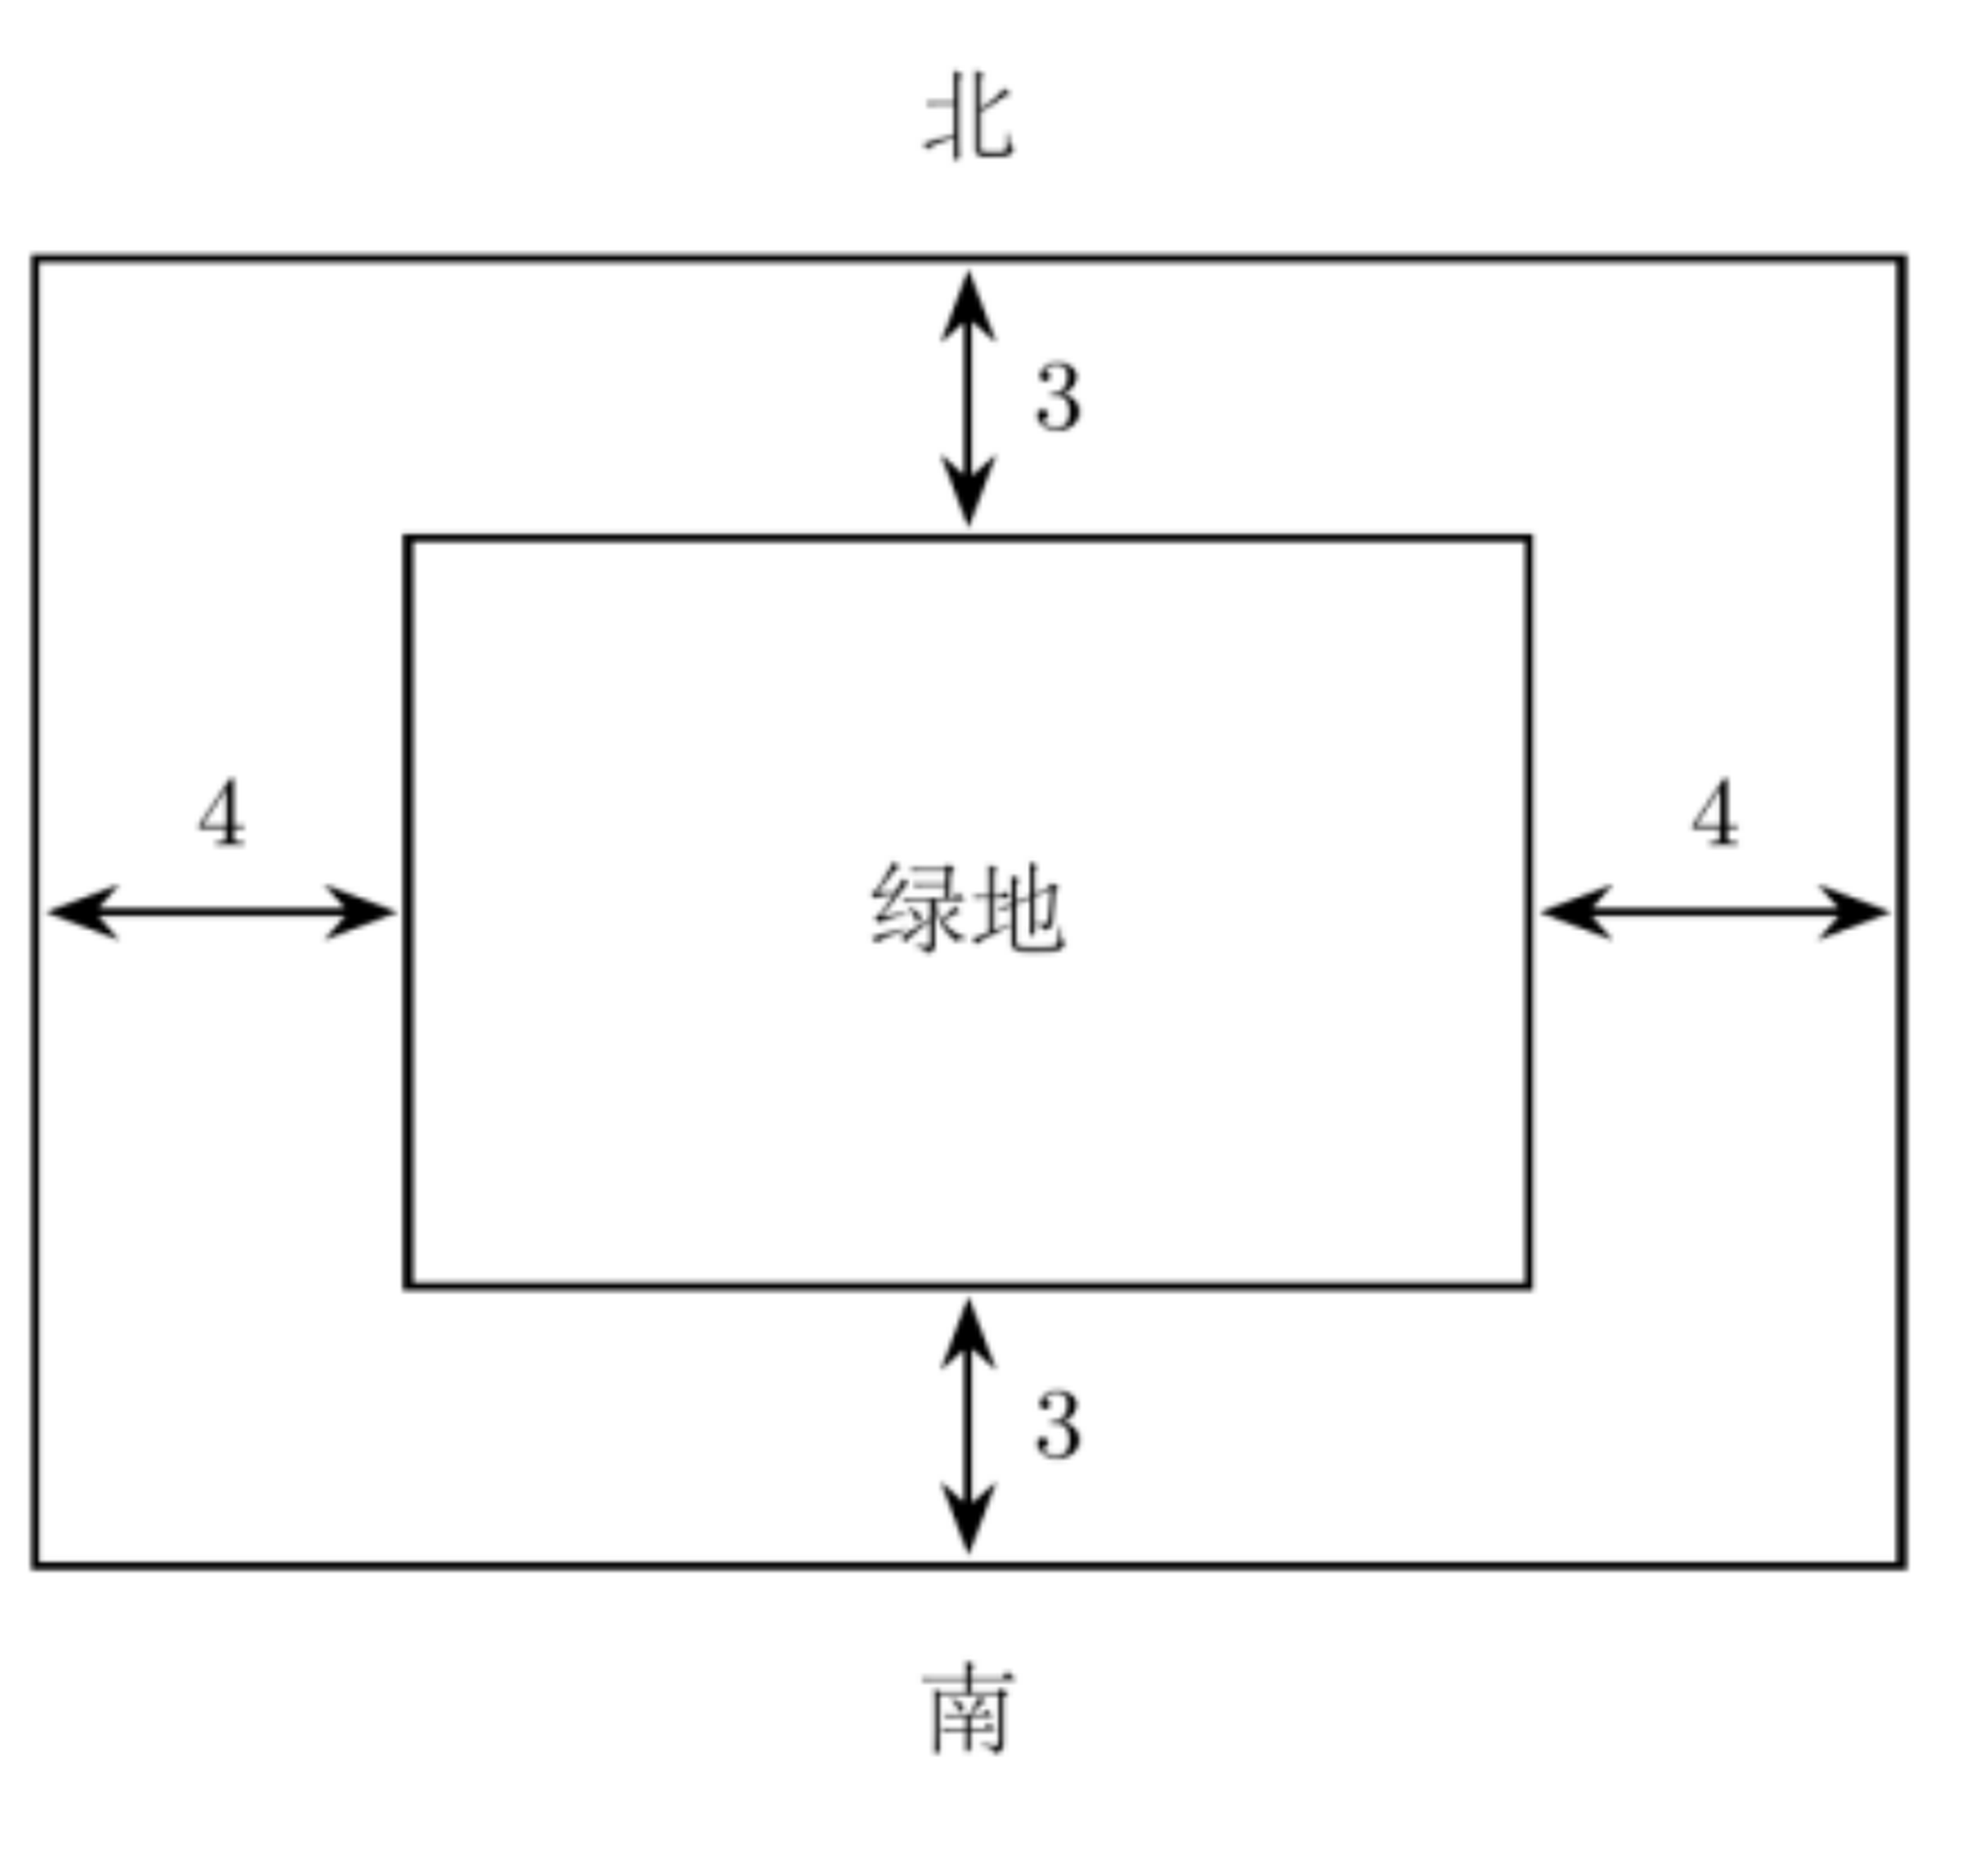
\includegraphics[width=0.32\textwidth]{figures/gao129_q19.png}
\end{center}

(1) 将 $S$ 表示为 $x$ 的函数；

(2) 试确定绿地东西方向的边长和南北方向的边长，使人行道的占地面积最小，并求出人行道的占地最小面积（结果精确到 0.1 米）

\ifanswer
\solbegin
\step{(1) 绿地南北方向的边长为 $\dfrac{1000}{x}$ 米，$x>0$.}
\step{外矩形东西、南北方向的边长分别为 $x+8$ 米、$\dfrac{1000}{x}+6$ 米.}
\step{因此 $S=(x+8)\left(\dfrac{1000}{x}+6\right)-1000=6x+\dfrac{8000}{x}+48, x>0$.}
\step{(2) 因为 $x>0,S=6x+\dfrac{8000}{x}+48\geqslant2\sqrt{6x\cdot\dfrac{8000}{x}}+48=48+80\sqrt{30}$.}
\step{等号当且仅当 $6x=\dfrac{8000}{x}$，即 $x=\dfrac{20\sqrt{30}}{3}\approx36.5$ 时成立，}
\step{此时绿地南北方向的边长为 $\dfrac{1000}{x}=\dfrac{1000}{\dfrac{20\sqrt{30}}{3}}=5\sqrt{30}\approx27.4$（米），}
\step{所以绿地东西方向、南北方向的边长分别约为 36.5 米、27.4 米时，}
\step{人行道的占地面积最小，最小面积为 $S_{min}=48+80\sqrt{30}\approx486.2$ 平方米.}
\solend
\fi

\item 已知集合 $A=\{x\mid x^2-3x+2=0\},B=\{x\mid x^2-ax+a-1=0\}$，

$C=\{x\mid x^2+2(m+1)x+m^2-5=0\}$.

(1) 若 $A=B$，求实数 $a$ 的值；

(2) 若 $B=\{1\}$，求实数 $a$ 的值；

(3) 若 $A\cap C=C$，求实数 $m$ 的取值范围.

\ifanswer
\solbegin
\step{(1) $A=\{1,2\}$，且 $x^2-ax+a-1=(x-1)(x-a+1)$，所以 $B=\{1,a-1\}$，}
\step{因此 $A=B\Leftrightarrow a-1=2\Leftrightarrow a=3$.}
\step{(2) $B=\{1\}$ 表示原方程只有一个不同的实数根，}
\step{得 $a-1=1$，即 $a=2$.}
\step{当 $a=2$ 时，原方程为 $(x-1)^2=0$，符合题意.}
\step{(3) $A\cap C=C\Leftrightarrow C\subseteq\{1,2\}$，}
\step{方程的判别式为 $\Delta=[2(m+1)]^2-4(m^2-5)=8(m+3)$.}
\step{当 $m<-3$ 时，$\Delta<0, C=\varnothing$，满足条件.}
\step{当 $m=-3$ 时，原方程为 $(x-2)^2=0, C=\{2\}$，满足条件.}
\step{当 $m>-3$ 时，方程有两个不同的实数根，必须有 $C=\{1,2\}$，}
\step{由韦达定理，$\begin{cases}-2(m+1)=1+2=3\\m^2-5=1\cdot2=2\end{cases}$，}
\step{第一式得 $m=-\dfrac52$，但此时 $m^2-5=\dfrac54\neq2$，不合题意.}
\step{因此 $m$ 的取值范围为 $(-\infty,-3]$.}
\solend
\fi

\item 设函数 $f(x)=ax^2+(1-a)x+a-2(a\in\R)$.

(1) 若关于 $x$ 的不等式 $f(x)\leqslant0$ 的解集为 $\left[0,\dfrac12\right]$，求实数 $a$ 的值；

(2) 若不等式 $f(x)\geqslant-2$ 对于实数 $a\in[-1,1]$ 时恒成立，求 $x$ 的取值范围；

(3) 解关于 $x$ 的不等式：$f(x)<a-1$.

\ifanswer
\solbegin
\step{(1) 由题意得 $0,\dfrac12$ 是方程 $ax^2+(1-a)x+a-2=0$ 的两个根，}
\step{则 $\begin{cases}0+\dfrac12=-\dfrac{1-a}{a}\\0\times\dfrac12=\dfrac{a-2}{a}\end{cases}\Rightarrow a=2$；}
\step{(2) $ax^2+(1-a)x+a-2\geqslant-2\Rightarrow a(x^2-x+1)+x\geqslant0$ 对 $a\in[-1,1]$ 恒成立，}
\step{则 $\begin{cases}-(x^2-x+1)+x\geqslant0\\(x^2-x+1)+x\geqslant0\end{cases}\Rightarrow\begin{cases}x=1\\x\in\R\end{cases}\Rightarrow x=1$，则 $x$ 的取值范围为 $\{1\}$；}
\step{(3) $f(x)<a-1$ 等价于 $ax^2+(1-a)x-1<0$，}
\step{当 $a=0$ 时，不等式可化为 $x<1$，解集为 $\{x\mid x<1\}$，}
\step{当 $a>0$ 时，不等式可化为 $(ax+1)(x-1)<0$，解集为 $\{x\mid -\dfrac1a<x<1\}$；}
\step{当 $a<0$ 时，不等式化为 $(ax+1)(x-1)<0$，}
\step{①当 $a=-1$ 时，$-\dfrac1a=1$，不等式的解集为 $\{x\mid x\neq1\}$；}
\step{②当 $-1<a<0$ 时，$-\dfrac1a>1$，不等式的解集为 $\{x\mid x<1$ 或 $x>-\dfrac1a\}$；}
\step{③当 $a<-1$ 时，$-\dfrac1a<1$，不等式的解集为 $\{x\mid x<-\dfrac1a$ 或 $x>1\}$；}
\step{综上，当 $a<-1$ 时，解集为 $\{x\mid x<-\dfrac1a$ 或 $x>1\}$；}
\step{当 $a=-1$ 时，解集为 $\{x\mid x\neq1\}$；}
\step{当 $-1<a<0$ 时，解集为 $\{x\mid x<1$ 或 $x>-\dfrac1a\}$；}
\step{当 $a=0$ 时，解集为 $\{x\mid x<1\}$；}
\step{当 $a>0$ 时，解集为 $\{x\mid -\dfrac1a<x<1\}$.}
\solend
\fi

\end{enumerate}

\end{document}
"
% 紧凑版：xelatex "\def\iscompact{1}% 高一129_立达中学_期中.tex
%   —— 高一上数学"2026-2027 年立达中学高一上期中"（试卷版/答案版）
% 试卷版：xelatex 高一129_立达中学_期中.tex
% 答案版：xelatex "\def\isanswer{1}% 高一129_立达中学_期中.tex
%   —— 高一上数学"2026-2027 年立达中学高一上期中"（试卷版/答案版）
% 试卷版：xelatex 高一129_立达中学_期中.tex
% 答案版：xelatex "\def\isanswer{1}% 高一129_立达中学_期中.tex
%   —— 高一上数学"2026-2027 年立达中学高一上期中"（试卷版/答案版）
% 试卷版：xelatex 高一129_立达中学_期中.tex
% 答案版：xelatex "\def\isanswer{1}\input{高一129_立达中学_期中.tex}"
% 紧凑版：xelatex "\def\iscompact{1}\input{高一129_立达中学_期中.tex}"
%
% 原始材料：微信公众号"魔都数学加油站"文章，作者破晓，2026-11-12 18:56 发布；
% 连载"27学年高一129"，原文标题"27学年高一129——2026-2027年上海市立达中学高一上期中"；
% 原文链接：https://mp.weixin.qq.com/s/gJhGsOBiWi7gW62u8EWLYA。
% 正文为 8 张 PNG 页（01、02、03、05、06 为 4762x6735，04、07、08 为 2560x3620），
% 题目下印有【解析】或【答案】，为讲评版。题目、解析均据原图转录；
% 卷面粉红色水印"魔都数学加油站"及公众号页脚未录入。全卷仅第 19 题有 1 幅插图。
%
% 卷首标题：原卷印作"2026-2027 年立达中学高一上期中"（公众号标题中的"上海市"
% 卷面标题行没有，本稿照卷面），年份区间按全稿惯例排 en dash；原卷未印副标题，
% 本卷为期中卷、跨集合与常用逻辑用语／不等式／函数三章，按题目内容标为
% "集合与常用逻辑用语、不等式、函数"（与 125、126 同为期中卷，口径相同）：
% 集合与逻辑见 Q3、Q4、Q13、Q20，不等式见 Q5、Q6、Q7、Q9、Q10、Q11、Q12、
% Q14、Q15、Q16、Q17、Q18、Q21，函数（含二次函数、基本不等式应用）见 Q8、Q19、Q21。
%
% 与原卷的排版差异：
%   ① 原文从第 3 题起，填空题编号为 3—12、选择题为 13—16、解答题为 17—21，本稿保留原题号；
%   ② 原卷每题下直接印【解析】／【答案】，本稿按全稿惯例置于答案版；第 3、5 题只印
%      【答案】，另提 \ans{}；第 13—16 题答案均在【解析】末句"故选 …"，题干括号内留空、
%      不另提 \ans{}；四道选择题括号内原卷均未印答案；
%   ③ 原卷未印副标题，本稿按"知识模块"口径补出（见上"卷首标题"）；
%   ④ 原卷填空横线按全稿惯例排为 \blankline[4.4em]；选择题括号排 \mbox{（\quad）}、
%      选项段前按惯例加 \keepwithprev；解答题不留作答区（原卷为讲评版，与 109—128 同）；
%   ⑤ 原卷数集排斜体 $R$，按全稿惯例改 \R；绝对值排 \lvert…\rvert，集合描述竖线排 \mid；
%      不等号按全稿惯例排 \leqslant／\geqslant；子题标号原卷一律用半角括号 (1)(2)(3)，本稿照录；
%   ⑥ 原卷第 19 题插图浮排在 Q18 解析右侧、"19."题干之上，本稿按体例就近置于 Q19
%      题干"如图所示"之后（居中 \includegraphics），图取原卷截图去水印；题前按惯例加
%      \needvspace{7cm} 守卫（照 高一120／127 成例），保证"题干 + 图"整块不被页边界切开；
%   ⑦ 原卷 Q8 解析续头印在第 2 页页首、Q17 解析续头印在第 5 页页首、Q19 题干续在第 6 页、
%      Q20 解析跨 6—7 页、Q21 解析续头印在第 8 页页首，本稿按题合并连续排版；
%      末页第 8 页为 Q21 解析的续尾，按实际印刷行单列（照 高一127 第 09 页续尾成例）。
%
% 判别式字形：第 8 题解析 $\Delta=m^2+4m>0$、第 10 题解析 $\Delta=k^2+6k=k(k+6)<0$、
%   第 20 题 (3) 解析 $\Delta=[2(m+1)]^2-4(m^2-5)=8(m+3)$ 三处原卷均排 $\Delta$
%   （等腰、高；回原图逐处放大核对、三处字形一致），照录 \Delta；全卷未出现 \triangle
%   （等边、扁）。
%
% 子集符号：第 13 题 ② $\{0,1,2\}\subseteq\{2,1,0\}$、③ $\varnothing\subseteq\{0,1,2\}$，
%   第 17 题 (2)② $B\subseteq A$、$B\subseteq(3,+\infty)$，第 20 题 (3) $C\subseteq\{1,2\}$
%   均印带下划线，照录 \subseteq；全卷未出现单线 \subset（回原图放大逐处确认）。
%
% 原卷存疑照录：
%   第 15 题解析"即 $m=4$，$n=3$ 时取等号"与题干 $\dfrac1m+n=1$、等号条件
%     $mn=\dfrac9{mn}$ 均不一致（按题应为 $n=\dfrac34$），照录、未统一；
%   第 18 题 (1) 题干"设 $M=2x^2+3x-1,N=7x-3$ 比较 $M$ 与 $N$ 两个数的大小"
%     两式间用半角逗号、且"$N=7x-3$"后无标点直接接"比较"，照录；
%   第 11 题解析"$1-x+2x-1=-(3x-2), 4x=2, x=\dfrac12$"、第 14 题解析
%     "$a=2, b=1, c=4, d=0$"、第 19 题解析"$6x+\dfrac{8000}{x}+48, x>0$"、
%     第 20 题解析"$\Delta<0, C=\varnothing$"与"$(x-2)^2=0, C=\{2\}$"、
%     第 12 题解析"$(x+y)^2=3+t\geqslant0,(x-y)^2=3-3t\geqslant0$"等处数学式内
%     用半角逗号，照录；
%   第 19 题题干"如图所示（图中单位：米）设绿地东西方向的边长为 $x$"在右括号后
%     无标点直接续"设"，照录；
%   第 21 题 (3) 解析先按 $a>0$、$a=0$、$a<0$ 分述解集，又在"综上"处重列全部
%     五类（含已给出的 $a>0$、$a=0$），照录；
%   第 21 题 (2) 题干与解析均作 $f(x)\geqslant-2$（与 $a(x^2-x+1)+x\geqslant0$ 相符），
%     照录，勿误读为 $f(x)\geqslant2$。
%
% 行数复核：逐题数 \step 条数，合计 93 条（Q3：0；Q4：2；Q5：0；Q6：3；Q7：3；
% Q8：2；Q9：4；Q10：3；Q11：5；Q12：5；Q13：1；Q14：3；Q15：3；Q16：7；
% Q17：7；Q18：8；Q19：8；Q20：13；Q21：16），与原卷印刷行逐题相等
% （cases 块作一个印刷行计）。第 3、5 题只印【答案】，提 \ans{}，不计入 \step 账；
% 四道选择题答案均在解析末句，括号内留空、不另提 \ans{}。
%
\documentclass[a4paper,11pt]{article}
\usepackage{common}

\begin{document}

\examtitlest[3]{2026--2027 年立达中学高一上期中}{集合与常用逻辑用语、不等式、函数}

\bigsec{一、填空题}

\begin{enumerate}
\setcounter{enumi}{2}

\item 若 $A=\{x\mid -3<x\leqslant2\},B=\{x\mid 1<x\leqslant3\}$，则 $A\cup B=$\blankline[4.4em].

\ifanswer
\ans{$(-3,3]$}
\fi

\item 若 $A$ 是 $B$ 的必要非充分条件，$B$ 是 $C$ 的充要条件，$C$ 是 $D$ 的必要非充分条件，则 $D$ 是 $A$ 的\blankline[4.4em]条件.

\ifanswer
\solbegin
\step{$D\Rightarrow C\Leftrightarrow B\Rightarrow A$，且 $A\nRightarrow B$，因此 $D\Rightarrow A$ 且 $A\nRightarrow D$，}
\step{故 $D$ 是 $A$ 的充分非必要条件.}
\solend
\fi

\item 不等式 $\dfrac1x<1$ 的解集为\blankline[4.4em].

\ifanswer
\ans{$(-\infty,0)\cup(1,+\infty)$}
\fi

\item 已知正实数 $x$、$y$ 满足 $2x+y=2$，则 $xy$ 的最大值为\blankline[4.4em].

\ifanswer
\solbegin
\step{因为 $x>0$，$y>0$，所以 $2x+y\geqslant2\sqrt{2xy}$（当且仅当 $2x=y$ 时，取等号），}
\step{又因为 $2x+y=2$，所以 $2\geqslant2\sqrt{2xy}$（当且仅当 $2x=y$ 时，取等号），}
\step{即 $xy\leqslant\dfrac12$，则 $xy$ 的最大值为 $\dfrac12$.}
\solend
\fi

\item 已知 $x\in\R$，函数 $y=\lvert x+2\rvert+\lvert x-3\rvert$ 的最小值为\blankline[4.4em].

\ifanswer
\solbegin
\step{由 $\lvert x+2\rvert+\lvert x-3\rvert\geqslant\lvert(x+2)-(x-3)\rvert=5$，}
\step{当且仅当 $(x+2)(x-3)\leqslant0$，即 $-2\leqslant x\leqslant3$ 时，上式取等号，}
\step{则函数 $y=\lvert x+2\rvert+\lvert x-3\rvert$ 的最小值是 5.}
\solend
\fi

\item 已知实系数一元二次方程 $x^2+mx-m=0$ 的两根分别为 $x_1,x_2$，且 $\lvert x_1-x_2\rvert=\sqrt{21}$，实数 $m$ 的值为\blankline[4.4em].

\ifanswer
\solbegin
\step{由题意得 $\Delta=m^2+4m>0$，解得 $m>0$ 或 $m<-4,x_1+x_2=-m,x_1x_2=-m$，}
\step{则 $\lvert x_1-x_2\rvert=\sqrt{(x_1+x_2)^2-4x_1x_2}=\sqrt{m^2+4m}=\sqrt{21}$，解得 $m=-7$ 或 $3$.}
\solend
\fi

\item 已知不等式 $ax^2-5x+b>0$ 的解集是 $\{x\mid -3<x<-2\}$，则不等式 $bx^2-5x+a>0$ 的解集是\blankline[4.4em].

\ifanswer
\solbegin
\step{$ax^2-5x+b=a(x+3)(x+2)$，比较系数得 $5a=-5,b=6a$，}
\step{即 $a=-1,b=-6$.}
\step{$bx^2-5x+a>0\Leftrightarrow(3x+1)(2x+1)<0\Leftrightarrow-\dfrac12<x<-\dfrac13$，}
\step{故解集为 $\left\{x\mid -\dfrac12<x<-\dfrac13\right\}$.}
\solend
\fi

\item 不等式 $4kx^2+kx-\dfrac38<0$ 对于一切实数 $x$ 都成立，则实数 $k$ 的取值范围是\blankline[4.4em].

\ifanswer
\solbegin
\step{$k=0$ 时，不等式恒成立；}
\step{$k\neq0$ 时，须 $4k<0$ 且 $\Delta=k^2+6k=k(k+6)<0$，解得 $-6<k<0$.}
\step{因此 $k\in(-6,0]$.}
\solend
\fi

\item 设 $x\in\R$，方程 $\lvert 1-x\rvert+\lvert 2x-1\rvert=\lvert 3x-2\rvert$ 的解集为\blankline[4.4em].

\ifanswer
\solbegin
\step{当 $x\leqslant\dfrac12$ 时，方程化为 $1-x-(2x-1)=-(3x-2)$，$2-3x=-3x+2$，恒成立，}
\step{当 $\dfrac12<x\leqslant\dfrac23$ 时，方程化为 $1-x+2x-1=-(3x-2), 4x=2, x=\dfrac12$，不合题意，}
\step{当 $\dfrac23<x\leqslant1$ 时，方程化为 $1-x+2x-1=3x-2$，$2x=2$，解得 $x=1$，}
\step{当 $x>1$ 时，方程化为 $-(1-x)+2x-1=3x-2$，$3x-2=3x-2$，恒成立，}
\step{综上所述，$\lvert 1-x\rvert+\lvert 2x-1\rvert=\lvert 3x-2\rvert$ 的解集为 $\left(-\infty,\dfrac12\right]\cup[1,+\infty)$.}
\solend
\fi

\item 已知非零实数 $x,y$ 满足 $x^2+xy+y^2=3$，则 $x^2-xy+y^2$ 的取值范围是\blankline[4.4em].

\ifanswer
\solbegin
\step{令 $t=xy\neq0$，由 $(x+y)^2=3+t\geqslant0,(x-y)^2=3-3t\geqslant0$，}
\step{得 $t\in[-3,0)\cup(0,1]$.}
\step{对上述任意 $t$，联立 $x+y=\sqrt{3+t},x-y=\sqrt{3-3t}$，所得 $x,y$ 满足原条件，}
\step{因此上述 $t$ 均可取到.}
\step{于是 $x^2-xy+y^2=3-2t$ 的取值范围为 $[1,3)\cup(3,9]$.}
\solend
\fi

\end{enumerate}

\bigsec{二、选择题}

\begin{enumerate}
\setcounter{enumi}{12}

\item 下列各式中，正确的个数是\mbox{（\quad）}

① $\{0\}\in\{0,1,2\}$；② $\{0,1,2\}\subseteq\{2,1,0\}$；③ $\varnothing\subseteq\{0,1,2\}$；④ $\varnothing=\{0\}$；⑤ $\{0,1\}=\{(0,1)\}$；

⑥ $0=\{0\}$.

\keepwithprev
A. $1$\qquad\qquad B. $2$\qquad\qquad C. $3$\qquad\qquad D. $4$

\ifanswer
\solbegin
\step{①不正确，②正确，③正确，④不正确，⑤不正确，⑥不正确. 故选 $B$.}
\solend
\fi

\item 下列四个命题中，为真命题的是\mbox{（\quad）}

\keepwithprev
A. 若 $a>b$，则 $ac^2>bc^2$\qquad\qquad B. 若 $a>b,c>d$，则 $a-c>b-d$

C. 若 $ac^2>bc^2$，则 $a>b$\qquad\qquad D. 若 $a>b$，则 $\dfrac1a<\dfrac1b$

\ifanswer
\solbegin
\step{C 中，$(a-b)c^2>0$，必有 $c^2>0$ 且 $a-b>0$，即 $a>b$.}
\step{A 取 $c=0$；B 取 $a=2, b=1, c=4, d=0$；D 取 $a=1, b=-1$，均不成立.}
\step{故选 $C$.}
\solend
\fi

\item 已知 $m$、$n\in(0,+\infty)$，$\dfrac1m+n=1$，则 $m+\dfrac9n$ 的最小值为\mbox{（\quad）}

\keepwithprev
A. $13$\qquad\qquad B. $16$\qquad\qquad C. $3$\qquad\qquad D. $6$

\ifanswer
\solbegin
\step{因为 $m$、$n\in(0,+\infty)$，$\dfrac1m+n=1$，}
\step{所以 $m+\dfrac9n=(m+\dfrac9n)(\dfrac1m+n)=10+mn+\dfrac9{mn}\geqslant10+2\sqrt{mn\cdot\dfrac9{mn}}=16$，}
\step{当且仅当 $mn=\dfrac9{mn}$，即 $m=4$，$n=3$ 时取等号. 故选 $B$.}
\solend
\fi

\item 下列不等式：① $\left\lvert x+\dfrac1x\right\rvert\geqslant2$；② $x^2+2x+1>0$；③ $\lvert x\rvert+\lvert x-1\rvert\geqslant1$；④ $\dfrac{x}{x^2+x+1}<1$；

解集为 $\R$ 的不等式的个数是\mbox{（\quad）}

\keepwithprev
A. $0$\qquad\qquad B. $1$\qquad\qquad C. $2$\qquad\qquad D. $3$

\ifanswer
\solbegin
\step{对于①，当 $x=0$ 时，$\dfrac1x$ 无意义，故 $\left\lvert x+\dfrac1x\right\rvert\geqslant2$ 的解集不是 $\R$，错误；}
\step{对于②，$x^2+2x+1=(x+1)^2\geqslant0$，当 $x=-1$ 取到等号，解集不是 $\R$，故错误；}
\step{对于③，$\lvert x\rvert+\lvert x-1\rvert\geqslant\lvert x-(x-1)\rvert=1$，当 $x(x-1)\leqslant0$ 时取等号，解集为 $\R$，}
\step{故正确；}
\step{对于④，由于 $x^2+x+1>0$ 恒成立，}
\step{故 $\dfrac{x}{x^2+x+1}<1$ 等价于 $x<x^2+x+1\Rightarrow x^2+1>0$ 恒成立，故解集为 $\R$，正确，}
\step{故正确的有③④，故选 $C$.}
\solend
\fi

\end{enumerate}

\bigsec{三、解答题}

\begin{enumerate}
\setcounter{enumi}{16}

\item (1) 解不等式组 $\begin{cases}\dfrac{x+3}{x+1}\leqslant2\\\lvert 2x-3\rvert\leqslant2\end{cases}$.

(2) 已知集合 $A=\{x\mid -x+3<0\},B=\{x\mid a\leqslant x\leqslant a+3\}$.

①当 $a=2$，求集合 $A\cap B$；

②若 $A\cup B=A$，求实数 $a$ 的取值范围.

\ifanswer
\solbegin
\step{(1) 由 $\begin{cases}\dfrac{x+3}{x+1}\leqslant2\\\lvert 2x-3\rvert\leqslant2\end{cases}$ 得 $\begin{cases}\dfrac{x+3-2x-2}{x+1}\leqslant0\\-2\leqslant2x-3\leqslant2\end{cases}$，即 $\begin{cases}\dfrac{-x+1}{x+1}\leqslant0\\1\leqslant2x\leqslant5\end{cases}$，则 $\begin{cases}\dfrac{x-1}{x+1}\geqslant0\\\dfrac12\leqslant x\leqslant\dfrac52\end{cases}$，}
\step{解得 $1\leqslant x\leqslant\dfrac52$，即原不等式组的解集为 $\left[1,\dfrac52\right]$.}
\step{(2) $-x+3<0\Leftrightarrow x>3$，所以 $A=(3,+\infty)$.}
\step{①当 $a=2$ 时，$B=[2,5], A\cap B=(3,+\infty)\cap[2,5]=(3,5]$.}
\step{②$A\cup B=A\Leftrightarrow B\subseteq A$.}
\step{因为 $B=[a,a+3]$，且左端点 $a\in B$，所以 $B\subseteq(3,+\infty)\Leftrightarrow a>3$，}
\step{实数 $a$ 的取值范围为 $(3,+\infty)$.}
\solend
\fi

\item (1) 设 $M=2x^2+3x-1,N=7x-3$ 比较 $M$ 与 $N$ 两个数的大小.

(2) 解关于 $x$ 的不等式：$x^2-(a+3)x+3a<0$，$a\in\R$.

\ifanswer
\solbegin
\step{(1) $M-N=2x^2+3x-1-(7x-3)=2(x-1)^2$.}
\step{$x=1$ 时，$M-N=0$，即 $M=N$.}
\step{$x\neq1$ 时，$M-N>0$，即 $M>N$.}
\step{(2) 不等式 $x^2-(a+3)x+3a<0$ 可化为 $(x-3)(x-a)<0$，}
\step{不等式对应方程的解为 $a$ 和 3，}
\step{当 $a<3$ 时，不等式 $x^2-(a+3)x+3a<0$ 的解集为 $(a,3)$，}
\step{当 $a=3$ 时，不等式 $x^2-(a+3)x+3a<0$ 的解集为 $\varnothing$，}
\step{当 $a>3$ 时，不等式 $x^2-(a+3)x+3a<0$ 的解集为 $(3,a)$.}
\solend
\fi

% 第 19 题是"题干 + 图"约 7cm 的一整块，答案版实测断点落在题干之后（图被推到次页页首），
% 照 高一120／127 成例在题前先量一次页高，不够就把"题干 + 图"整块一起挪到次页。
\needvspace{7cm}
\item 某新建居民小区欲建一面积为 1000 平方米的矩形绿地，在绿地四周铺设人行道，设计要求绿地南北两侧人行道宽 3 米，东西两侧人行道宽 4 米，如图所示（图中单位：米）设绿地东西方向的边长为 $x$，人行道的占地面积为 $S$.

\begin{center}
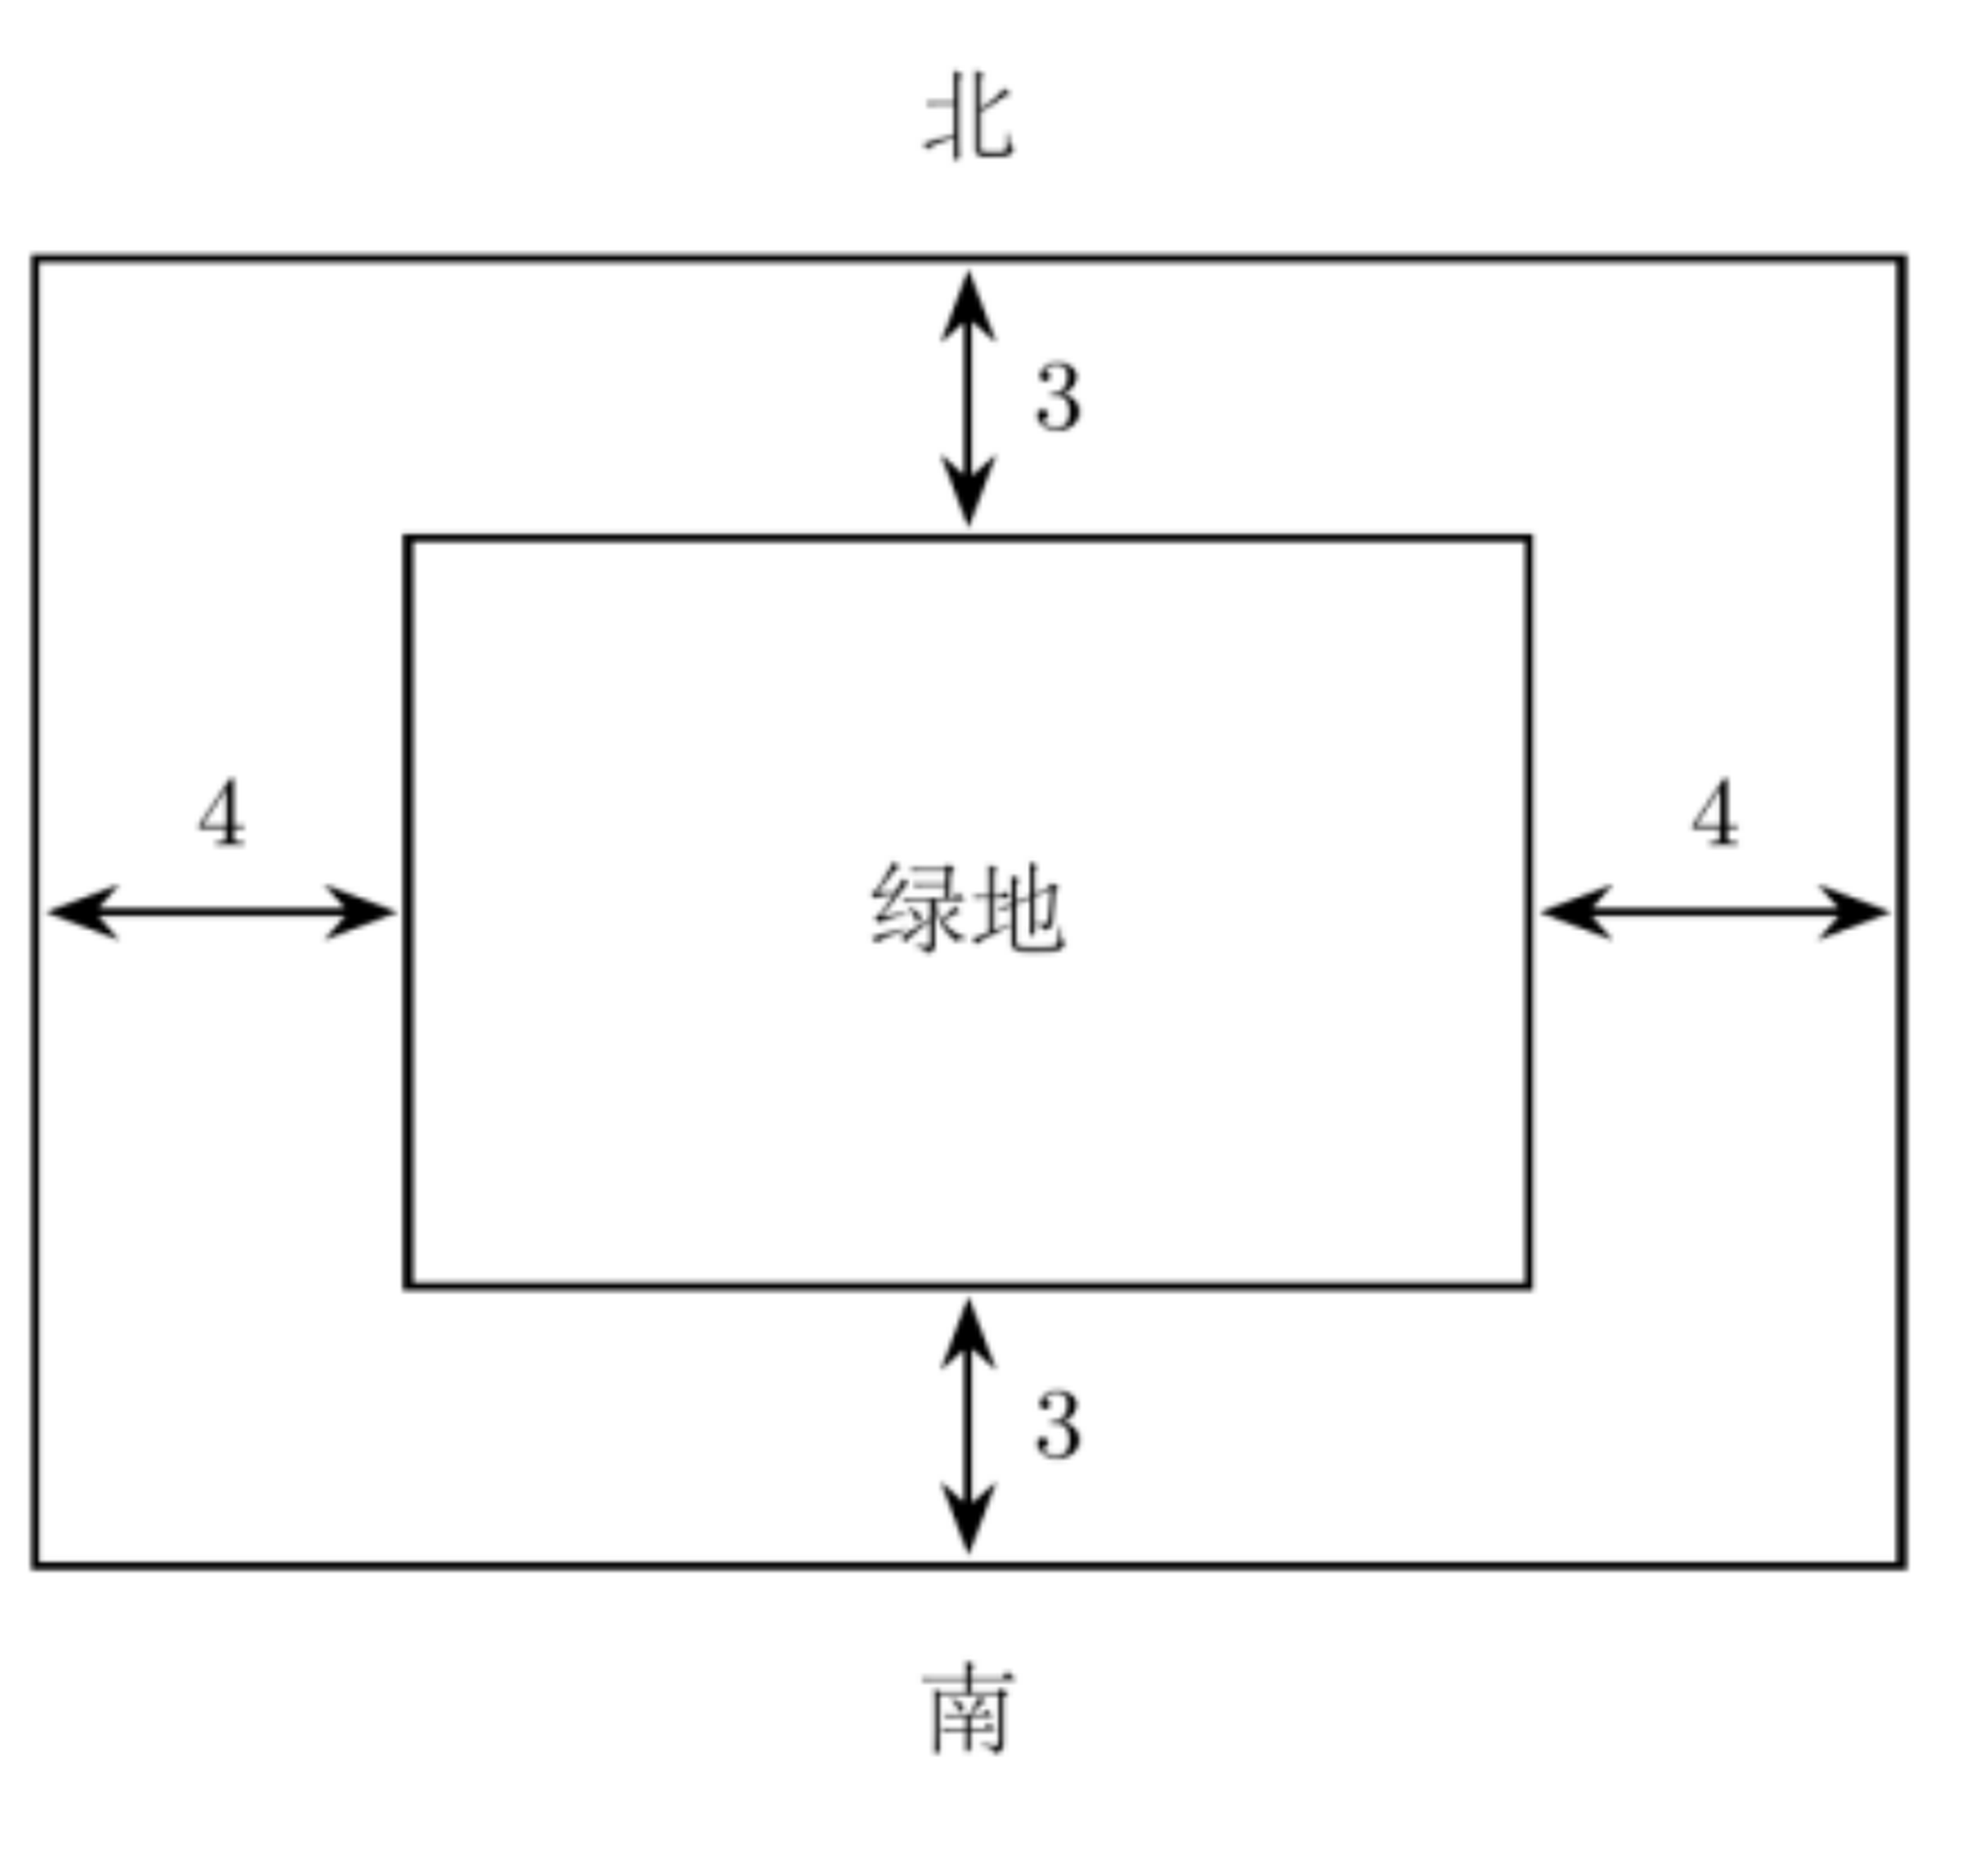
\includegraphics[width=0.32\textwidth]{figures/gao129_q19.png}
\end{center}

(1) 将 $S$ 表示为 $x$ 的函数；

(2) 试确定绿地东西方向的边长和南北方向的边长，使人行道的占地面积最小，并求出人行道的占地最小面积（结果精确到 0.1 米）

\ifanswer
\solbegin
\step{(1) 绿地南北方向的边长为 $\dfrac{1000}{x}$ 米，$x>0$.}
\step{外矩形东西、南北方向的边长分别为 $x+8$ 米、$\dfrac{1000}{x}+6$ 米.}
\step{因此 $S=(x+8)\left(\dfrac{1000}{x}+6\right)-1000=6x+\dfrac{8000}{x}+48, x>0$.}
\step{(2) 因为 $x>0,S=6x+\dfrac{8000}{x}+48\geqslant2\sqrt{6x\cdot\dfrac{8000}{x}}+48=48+80\sqrt{30}$.}
\step{等号当且仅当 $6x=\dfrac{8000}{x}$，即 $x=\dfrac{20\sqrt{30}}{3}\approx36.5$ 时成立，}
\step{此时绿地南北方向的边长为 $\dfrac{1000}{x}=\dfrac{1000}{\dfrac{20\sqrt{30}}{3}}=5\sqrt{30}\approx27.4$（米），}
\step{所以绿地东西方向、南北方向的边长分别约为 36.5 米、27.4 米时，}
\step{人行道的占地面积最小，最小面积为 $S_{min}=48+80\sqrt{30}\approx486.2$ 平方米.}
\solend
\fi

\item 已知集合 $A=\{x\mid x^2-3x+2=0\},B=\{x\mid x^2-ax+a-1=0\}$，

$C=\{x\mid x^2+2(m+1)x+m^2-5=0\}$.

(1) 若 $A=B$，求实数 $a$ 的值；

(2) 若 $B=\{1\}$，求实数 $a$ 的值；

(3) 若 $A\cap C=C$，求实数 $m$ 的取值范围.

\ifanswer
\solbegin
\step{(1) $A=\{1,2\}$，且 $x^2-ax+a-1=(x-1)(x-a+1)$，所以 $B=\{1,a-1\}$，}
\step{因此 $A=B\Leftrightarrow a-1=2\Leftrightarrow a=3$.}
\step{(2) $B=\{1\}$ 表示原方程只有一个不同的实数根，}
\step{得 $a-1=1$，即 $a=2$.}
\step{当 $a=2$ 时，原方程为 $(x-1)^2=0$，符合题意.}
\step{(3) $A\cap C=C\Leftrightarrow C\subseteq\{1,2\}$，}
\step{方程的判别式为 $\Delta=[2(m+1)]^2-4(m^2-5)=8(m+3)$.}
\step{当 $m<-3$ 时，$\Delta<0, C=\varnothing$，满足条件.}
\step{当 $m=-3$ 时，原方程为 $(x-2)^2=0, C=\{2\}$，满足条件.}
\step{当 $m>-3$ 时，方程有两个不同的实数根，必须有 $C=\{1,2\}$，}
\step{由韦达定理，$\begin{cases}-2(m+1)=1+2=3\\m^2-5=1\cdot2=2\end{cases}$，}
\step{第一式得 $m=-\dfrac52$，但此时 $m^2-5=\dfrac54\neq2$，不合题意.}
\step{因此 $m$ 的取值范围为 $(-\infty,-3]$.}
\solend
\fi

\item 设函数 $f(x)=ax^2+(1-a)x+a-2(a\in\R)$.

(1) 若关于 $x$ 的不等式 $f(x)\leqslant0$ 的解集为 $\left[0,\dfrac12\right]$，求实数 $a$ 的值；

(2) 若不等式 $f(x)\geqslant-2$ 对于实数 $a\in[-1,1]$ 时恒成立，求 $x$ 的取值范围；

(3) 解关于 $x$ 的不等式：$f(x)<a-1$.

\ifanswer
\solbegin
\step{(1) 由题意得 $0,\dfrac12$ 是方程 $ax^2+(1-a)x+a-2=0$ 的两个根，}
\step{则 $\begin{cases}0+\dfrac12=-\dfrac{1-a}{a}\\0\times\dfrac12=\dfrac{a-2}{a}\end{cases}\Rightarrow a=2$；}
\step{(2) $ax^2+(1-a)x+a-2\geqslant-2\Rightarrow a(x^2-x+1)+x\geqslant0$ 对 $a\in[-1,1]$ 恒成立，}
\step{则 $\begin{cases}-(x^2-x+1)+x\geqslant0\\(x^2-x+1)+x\geqslant0\end{cases}\Rightarrow\begin{cases}x=1\\x\in\R\end{cases}\Rightarrow x=1$，则 $x$ 的取值范围为 $\{1\}$；}
\step{(3) $f(x)<a-1$ 等价于 $ax^2+(1-a)x-1<0$，}
\step{当 $a=0$ 时，不等式可化为 $x<1$，解集为 $\{x\mid x<1\}$，}
\step{当 $a>0$ 时，不等式可化为 $(ax+1)(x-1)<0$，解集为 $\{x\mid -\dfrac1a<x<1\}$；}
\step{当 $a<0$ 时，不等式化为 $(ax+1)(x-1)<0$，}
\step{①当 $a=-1$ 时，$-\dfrac1a=1$，不等式的解集为 $\{x\mid x\neq1\}$；}
\step{②当 $-1<a<0$ 时，$-\dfrac1a>1$，不等式的解集为 $\{x\mid x<1$ 或 $x>-\dfrac1a\}$；}
\step{③当 $a<-1$ 时，$-\dfrac1a<1$，不等式的解集为 $\{x\mid x<-\dfrac1a$ 或 $x>1\}$；}
\step{综上，当 $a<-1$ 时，解集为 $\{x\mid x<-\dfrac1a$ 或 $x>1\}$；}
\step{当 $a=-1$ 时，解集为 $\{x\mid x\neq1\}$；}
\step{当 $-1<a<0$ 时，解集为 $\{x\mid x<1$ 或 $x>-\dfrac1a\}$；}
\step{当 $a=0$ 时，解集为 $\{x\mid x<1\}$；}
\step{当 $a>0$ 时，解集为 $\{x\mid -\dfrac1a<x<1\}$.}
\solend
\fi

\end{enumerate}

\end{document}
"
% 紧凑版：xelatex "\def\iscompact{1}% 高一129_立达中学_期中.tex
%   —— 高一上数学"2026-2027 年立达中学高一上期中"（试卷版/答案版）
% 试卷版：xelatex 高一129_立达中学_期中.tex
% 答案版：xelatex "\def\isanswer{1}\input{高一129_立达中学_期中.tex}"
% 紧凑版：xelatex "\def\iscompact{1}\input{高一129_立达中学_期中.tex}"
%
% 原始材料：微信公众号"魔都数学加油站"文章，作者破晓，2026-11-12 18:56 发布；
% 连载"27学年高一129"，原文标题"27学年高一129——2026-2027年上海市立达中学高一上期中"；
% 原文链接：https://mp.weixin.qq.com/s/gJhGsOBiWi7gW62u8EWLYA。
% 正文为 8 张 PNG 页（01、02、03、05、06 为 4762x6735，04、07、08 为 2560x3620），
% 题目下印有【解析】或【答案】，为讲评版。题目、解析均据原图转录；
% 卷面粉红色水印"魔都数学加油站"及公众号页脚未录入。全卷仅第 19 题有 1 幅插图。
%
% 卷首标题：原卷印作"2026-2027 年立达中学高一上期中"（公众号标题中的"上海市"
% 卷面标题行没有，本稿照卷面），年份区间按全稿惯例排 en dash；原卷未印副标题，
% 本卷为期中卷、跨集合与常用逻辑用语／不等式／函数三章，按题目内容标为
% "集合与常用逻辑用语、不等式、函数"（与 125、126 同为期中卷，口径相同）：
% 集合与逻辑见 Q3、Q4、Q13、Q20，不等式见 Q5、Q6、Q7、Q9、Q10、Q11、Q12、
% Q14、Q15、Q16、Q17、Q18、Q21，函数（含二次函数、基本不等式应用）见 Q8、Q19、Q21。
%
% 与原卷的排版差异：
%   ① 原文从第 3 题起，填空题编号为 3—12、选择题为 13—16、解答题为 17—21，本稿保留原题号；
%   ② 原卷每题下直接印【解析】／【答案】，本稿按全稿惯例置于答案版；第 3、5 题只印
%      【答案】，另提 \ans{}；第 13—16 题答案均在【解析】末句"故选 …"，题干括号内留空、
%      不另提 \ans{}；四道选择题括号内原卷均未印答案；
%   ③ 原卷未印副标题，本稿按"知识模块"口径补出（见上"卷首标题"）；
%   ④ 原卷填空横线按全稿惯例排为 \blankline[4.4em]；选择题括号排 \mbox{（\quad）}、
%      选项段前按惯例加 \keepwithprev；解答题不留作答区（原卷为讲评版，与 109—128 同）；
%   ⑤ 原卷数集排斜体 $R$，按全稿惯例改 \R；绝对值排 \lvert…\rvert，集合描述竖线排 \mid；
%      不等号按全稿惯例排 \leqslant／\geqslant；子题标号原卷一律用半角括号 (1)(2)(3)，本稿照录；
%   ⑥ 原卷第 19 题插图浮排在 Q18 解析右侧、"19."题干之上，本稿按体例就近置于 Q19
%      题干"如图所示"之后（居中 \includegraphics），图取原卷截图去水印；题前按惯例加
%      \needvspace{7cm} 守卫（照 高一120／127 成例），保证"题干 + 图"整块不被页边界切开；
%   ⑦ 原卷 Q8 解析续头印在第 2 页页首、Q17 解析续头印在第 5 页页首、Q19 题干续在第 6 页、
%      Q20 解析跨 6—7 页、Q21 解析续头印在第 8 页页首，本稿按题合并连续排版；
%      末页第 8 页为 Q21 解析的续尾，按实际印刷行单列（照 高一127 第 09 页续尾成例）。
%
% 判别式字形：第 8 题解析 $\Delta=m^2+4m>0$、第 10 题解析 $\Delta=k^2+6k=k(k+6)<0$、
%   第 20 题 (3) 解析 $\Delta=[2(m+1)]^2-4(m^2-5)=8(m+3)$ 三处原卷均排 $\Delta$
%   （等腰、高；回原图逐处放大核对、三处字形一致），照录 \Delta；全卷未出现 \triangle
%   （等边、扁）。
%
% 子集符号：第 13 题 ② $\{0,1,2\}\subseteq\{2,1,0\}$、③ $\varnothing\subseteq\{0,1,2\}$，
%   第 17 题 (2)② $B\subseteq A$、$B\subseteq(3,+\infty)$，第 20 题 (3) $C\subseteq\{1,2\}$
%   均印带下划线，照录 \subseteq；全卷未出现单线 \subset（回原图放大逐处确认）。
%
% 原卷存疑照录：
%   第 15 题解析"即 $m=4$，$n=3$ 时取等号"与题干 $\dfrac1m+n=1$、等号条件
%     $mn=\dfrac9{mn}$ 均不一致（按题应为 $n=\dfrac34$），照录、未统一；
%   第 18 题 (1) 题干"设 $M=2x^2+3x-1,N=7x-3$ 比较 $M$ 与 $N$ 两个数的大小"
%     两式间用半角逗号、且"$N=7x-3$"后无标点直接接"比较"，照录；
%   第 11 题解析"$1-x+2x-1=-(3x-2), 4x=2, x=\dfrac12$"、第 14 题解析
%     "$a=2, b=1, c=4, d=0$"、第 19 题解析"$6x+\dfrac{8000}{x}+48, x>0$"、
%     第 20 题解析"$\Delta<0, C=\varnothing$"与"$(x-2)^2=0, C=\{2\}$"、
%     第 12 题解析"$(x+y)^2=3+t\geqslant0,(x-y)^2=3-3t\geqslant0$"等处数学式内
%     用半角逗号，照录；
%   第 19 题题干"如图所示（图中单位：米）设绿地东西方向的边长为 $x$"在右括号后
%     无标点直接续"设"，照录；
%   第 21 题 (3) 解析先按 $a>0$、$a=0$、$a<0$ 分述解集，又在"综上"处重列全部
%     五类（含已给出的 $a>0$、$a=0$），照录；
%   第 21 题 (2) 题干与解析均作 $f(x)\geqslant-2$（与 $a(x^2-x+1)+x\geqslant0$ 相符），
%     照录，勿误读为 $f(x)\geqslant2$。
%
% 行数复核：逐题数 \step 条数，合计 93 条（Q3：0；Q4：2；Q5：0；Q6：3；Q7：3；
% Q8：2；Q9：4；Q10：3；Q11：5；Q12：5；Q13：1；Q14：3；Q15：3；Q16：7；
% Q17：7；Q18：8；Q19：8；Q20：13；Q21：16），与原卷印刷行逐题相等
% （cases 块作一个印刷行计）。第 3、5 题只印【答案】，提 \ans{}，不计入 \step 账；
% 四道选择题答案均在解析末句，括号内留空、不另提 \ans{}。
%
\documentclass[a4paper,11pt]{article}
\usepackage{common}

\begin{document}

\examtitlest[3]{2026--2027 年立达中学高一上期中}{集合与常用逻辑用语、不等式、函数}

\bigsec{一、填空题}

\begin{enumerate}
\setcounter{enumi}{2}

\item 若 $A=\{x\mid -3<x\leqslant2\},B=\{x\mid 1<x\leqslant3\}$，则 $A\cup B=$\blankline[4.4em].

\ifanswer
\ans{$(-3,3]$}
\fi

\item 若 $A$ 是 $B$ 的必要非充分条件，$B$ 是 $C$ 的充要条件，$C$ 是 $D$ 的必要非充分条件，则 $D$ 是 $A$ 的\blankline[4.4em]条件.

\ifanswer
\solbegin
\step{$D\Rightarrow C\Leftrightarrow B\Rightarrow A$，且 $A\nRightarrow B$，因此 $D\Rightarrow A$ 且 $A\nRightarrow D$，}
\step{故 $D$ 是 $A$ 的充分非必要条件.}
\solend
\fi

\item 不等式 $\dfrac1x<1$ 的解集为\blankline[4.4em].

\ifanswer
\ans{$(-\infty,0)\cup(1,+\infty)$}
\fi

\item 已知正实数 $x$、$y$ 满足 $2x+y=2$，则 $xy$ 的最大值为\blankline[4.4em].

\ifanswer
\solbegin
\step{因为 $x>0$，$y>0$，所以 $2x+y\geqslant2\sqrt{2xy}$（当且仅当 $2x=y$ 时，取等号），}
\step{又因为 $2x+y=2$，所以 $2\geqslant2\sqrt{2xy}$（当且仅当 $2x=y$ 时，取等号），}
\step{即 $xy\leqslant\dfrac12$，则 $xy$ 的最大值为 $\dfrac12$.}
\solend
\fi

\item 已知 $x\in\R$，函数 $y=\lvert x+2\rvert+\lvert x-3\rvert$ 的最小值为\blankline[4.4em].

\ifanswer
\solbegin
\step{由 $\lvert x+2\rvert+\lvert x-3\rvert\geqslant\lvert(x+2)-(x-3)\rvert=5$，}
\step{当且仅当 $(x+2)(x-3)\leqslant0$，即 $-2\leqslant x\leqslant3$ 时，上式取等号，}
\step{则函数 $y=\lvert x+2\rvert+\lvert x-3\rvert$ 的最小值是 5.}
\solend
\fi

\item 已知实系数一元二次方程 $x^2+mx-m=0$ 的两根分别为 $x_1,x_2$，且 $\lvert x_1-x_2\rvert=\sqrt{21}$，实数 $m$ 的值为\blankline[4.4em].

\ifanswer
\solbegin
\step{由题意得 $\Delta=m^2+4m>0$，解得 $m>0$ 或 $m<-4,x_1+x_2=-m,x_1x_2=-m$，}
\step{则 $\lvert x_1-x_2\rvert=\sqrt{(x_1+x_2)^2-4x_1x_2}=\sqrt{m^2+4m}=\sqrt{21}$，解得 $m=-7$ 或 $3$.}
\solend
\fi

\item 已知不等式 $ax^2-5x+b>0$ 的解集是 $\{x\mid -3<x<-2\}$，则不等式 $bx^2-5x+a>0$ 的解集是\blankline[4.4em].

\ifanswer
\solbegin
\step{$ax^2-5x+b=a(x+3)(x+2)$，比较系数得 $5a=-5,b=6a$，}
\step{即 $a=-1,b=-6$.}
\step{$bx^2-5x+a>0\Leftrightarrow(3x+1)(2x+1)<0\Leftrightarrow-\dfrac12<x<-\dfrac13$，}
\step{故解集为 $\left\{x\mid -\dfrac12<x<-\dfrac13\right\}$.}
\solend
\fi

\item 不等式 $4kx^2+kx-\dfrac38<0$ 对于一切实数 $x$ 都成立，则实数 $k$ 的取值范围是\blankline[4.4em].

\ifanswer
\solbegin
\step{$k=0$ 时，不等式恒成立；}
\step{$k\neq0$ 时，须 $4k<0$ 且 $\Delta=k^2+6k=k(k+6)<0$，解得 $-6<k<0$.}
\step{因此 $k\in(-6,0]$.}
\solend
\fi

\item 设 $x\in\R$，方程 $\lvert 1-x\rvert+\lvert 2x-1\rvert=\lvert 3x-2\rvert$ 的解集为\blankline[4.4em].

\ifanswer
\solbegin
\step{当 $x\leqslant\dfrac12$ 时，方程化为 $1-x-(2x-1)=-(3x-2)$，$2-3x=-3x+2$，恒成立，}
\step{当 $\dfrac12<x\leqslant\dfrac23$ 时，方程化为 $1-x+2x-1=-(3x-2), 4x=2, x=\dfrac12$，不合题意，}
\step{当 $\dfrac23<x\leqslant1$ 时，方程化为 $1-x+2x-1=3x-2$，$2x=2$，解得 $x=1$，}
\step{当 $x>1$ 时，方程化为 $-(1-x)+2x-1=3x-2$，$3x-2=3x-2$，恒成立，}
\step{综上所述，$\lvert 1-x\rvert+\lvert 2x-1\rvert=\lvert 3x-2\rvert$ 的解集为 $\left(-\infty,\dfrac12\right]\cup[1,+\infty)$.}
\solend
\fi

\item 已知非零实数 $x,y$ 满足 $x^2+xy+y^2=3$，则 $x^2-xy+y^2$ 的取值范围是\blankline[4.4em].

\ifanswer
\solbegin
\step{令 $t=xy\neq0$，由 $(x+y)^2=3+t\geqslant0,(x-y)^2=3-3t\geqslant0$，}
\step{得 $t\in[-3,0)\cup(0,1]$.}
\step{对上述任意 $t$，联立 $x+y=\sqrt{3+t},x-y=\sqrt{3-3t}$，所得 $x,y$ 满足原条件，}
\step{因此上述 $t$ 均可取到.}
\step{于是 $x^2-xy+y^2=3-2t$ 的取值范围为 $[1,3)\cup(3,9]$.}
\solend
\fi

\end{enumerate}

\bigsec{二、选择题}

\begin{enumerate}
\setcounter{enumi}{12}

\item 下列各式中，正确的个数是\mbox{（\quad）}

① $\{0\}\in\{0,1,2\}$；② $\{0,1,2\}\subseteq\{2,1,0\}$；③ $\varnothing\subseteq\{0,1,2\}$；④ $\varnothing=\{0\}$；⑤ $\{0,1\}=\{(0,1)\}$；

⑥ $0=\{0\}$.

\keepwithprev
A. $1$\qquad\qquad B. $2$\qquad\qquad C. $3$\qquad\qquad D. $4$

\ifanswer
\solbegin
\step{①不正确，②正确，③正确，④不正确，⑤不正确，⑥不正确. 故选 $B$.}
\solend
\fi

\item 下列四个命题中，为真命题的是\mbox{（\quad）}

\keepwithprev
A. 若 $a>b$，则 $ac^2>bc^2$\qquad\qquad B. 若 $a>b,c>d$，则 $a-c>b-d$

C. 若 $ac^2>bc^2$，则 $a>b$\qquad\qquad D. 若 $a>b$，则 $\dfrac1a<\dfrac1b$

\ifanswer
\solbegin
\step{C 中，$(a-b)c^2>0$，必有 $c^2>0$ 且 $a-b>0$，即 $a>b$.}
\step{A 取 $c=0$；B 取 $a=2, b=1, c=4, d=0$；D 取 $a=1, b=-1$，均不成立.}
\step{故选 $C$.}
\solend
\fi

\item 已知 $m$、$n\in(0,+\infty)$，$\dfrac1m+n=1$，则 $m+\dfrac9n$ 的最小值为\mbox{（\quad）}

\keepwithprev
A. $13$\qquad\qquad B. $16$\qquad\qquad C. $3$\qquad\qquad D. $6$

\ifanswer
\solbegin
\step{因为 $m$、$n\in(0,+\infty)$，$\dfrac1m+n=1$，}
\step{所以 $m+\dfrac9n=(m+\dfrac9n)(\dfrac1m+n)=10+mn+\dfrac9{mn}\geqslant10+2\sqrt{mn\cdot\dfrac9{mn}}=16$，}
\step{当且仅当 $mn=\dfrac9{mn}$，即 $m=4$，$n=3$ 时取等号. 故选 $B$.}
\solend
\fi

\item 下列不等式：① $\left\lvert x+\dfrac1x\right\rvert\geqslant2$；② $x^2+2x+1>0$；③ $\lvert x\rvert+\lvert x-1\rvert\geqslant1$；④ $\dfrac{x}{x^2+x+1}<1$；

解集为 $\R$ 的不等式的个数是\mbox{（\quad）}

\keepwithprev
A. $0$\qquad\qquad B. $1$\qquad\qquad C. $2$\qquad\qquad D. $3$

\ifanswer
\solbegin
\step{对于①，当 $x=0$ 时，$\dfrac1x$ 无意义，故 $\left\lvert x+\dfrac1x\right\rvert\geqslant2$ 的解集不是 $\R$，错误；}
\step{对于②，$x^2+2x+1=(x+1)^2\geqslant0$，当 $x=-1$ 取到等号，解集不是 $\R$，故错误；}
\step{对于③，$\lvert x\rvert+\lvert x-1\rvert\geqslant\lvert x-(x-1)\rvert=1$，当 $x(x-1)\leqslant0$ 时取等号，解集为 $\R$，}
\step{故正确；}
\step{对于④，由于 $x^2+x+1>0$ 恒成立，}
\step{故 $\dfrac{x}{x^2+x+1}<1$ 等价于 $x<x^2+x+1\Rightarrow x^2+1>0$ 恒成立，故解集为 $\R$，正确，}
\step{故正确的有③④，故选 $C$.}
\solend
\fi

\end{enumerate}

\bigsec{三、解答题}

\begin{enumerate}
\setcounter{enumi}{16}

\item (1) 解不等式组 $\begin{cases}\dfrac{x+3}{x+1}\leqslant2\\\lvert 2x-3\rvert\leqslant2\end{cases}$.

(2) 已知集合 $A=\{x\mid -x+3<0\},B=\{x\mid a\leqslant x\leqslant a+3\}$.

①当 $a=2$，求集合 $A\cap B$；

②若 $A\cup B=A$，求实数 $a$ 的取值范围.

\ifanswer
\solbegin
\step{(1) 由 $\begin{cases}\dfrac{x+3}{x+1}\leqslant2\\\lvert 2x-3\rvert\leqslant2\end{cases}$ 得 $\begin{cases}\dfrac{x+3-2x-2}{x+1}\leqslant0\\-2\leqslant2x-3\leqslant2\end{cases}$，即 $\begin{cases}\dfrac{-x+1}{x+1}\leqslant0\\1\leqslant2x\leqslant5\end{cases}$，则 $\begin{cases}\dfrac{x-1}{x+1}\geqslant0\\\dfrac12\leqslant x\leqslant\dfrac52\end{cases}$，}
\step{解得 $1\leqslant x\leqslant\dfrac52$，即原不等式组的解集为 $\left[1,\dfrac52\right]$.}
\step{(2) $-x+3<0\Leftrightarrow x>3$，所以 $A=(3,+\infty)$.}
\step{①当 $a=2$ 时，$B=[2,5], A\cap B=(3,+\infty)\cap[2,5]=(3,5]$.}
\step{②$A\cup B=A\Leftrightarrow B\subseteq A$.}
\step{因为 $B=[a,a+3]$，且左端点 $a\in B$，所以 $B\subseteq(3,+\infty)\Leftrightarrow a>3$，}
\step{实数 $a$ 的取值范围为 $(3,+\infty)$.}
\solend
\fi

\item (1) 设 $M=2x^2+3x-1,N=7x-3$ 比较 $M$ 与 $N$ 两个数的大小.

(2) 解关于 $x$ 的不等式：$x^2-(a+3)x+3a<0$，$a\in\R$.

\ifanswer
\solbegin
\step{(1) $M-N=2x^2+3x-1-(7x-3)=2(x-1)^2$.}
\step{$x=1$ 时，$M-N=0$，即 $M=N$.}
\step{$x\neq1$ 时，$M-N>0$，即 $M>N$.}
\step{(2) 不等式 $x^2-(a+3)x+3a<0$ 可化为 $(x-3)(x-a)<0$，}
\step{不等式对应方程的解为 $a$ 和 3，}
\step{当 $a<3$ 时，不等式 $x^2-(a+3)x+3a<0$ 的解集为 $(a,3)$，}
\step{当 $a=3$ 时，不等式 $x^2-(a+3)x+3a<0$ 的解集为 $\varnothing$，}
\step{当 $a>3$ 时，不等式 $x^2-(a+3)x+3a<0$ 的解集为 $(3,a)$.}
\solend
\fi

% 第 19 题是"题干 + 图"约 7cm 的一整块，答案版实测断点落在题干之后（图被推到次页页首），
% 照 高一120／127 成例在题前先量一次页高，不够就把"题干 + 图"整块一起挪到次页。
\needvspace{7cm}
\item 某新建居民小区欲建一面积为 1000 平方米的矩形绿地，在绿地四周铺设人行道，设计要求绿地南北两侧人行道宽 3 米，东西两侧人行道宽 4 米，如图所示（图中单位：米）设绿地东西方向的边长为 $x$，人行道的占地面积为 $S$.

\begin{center}
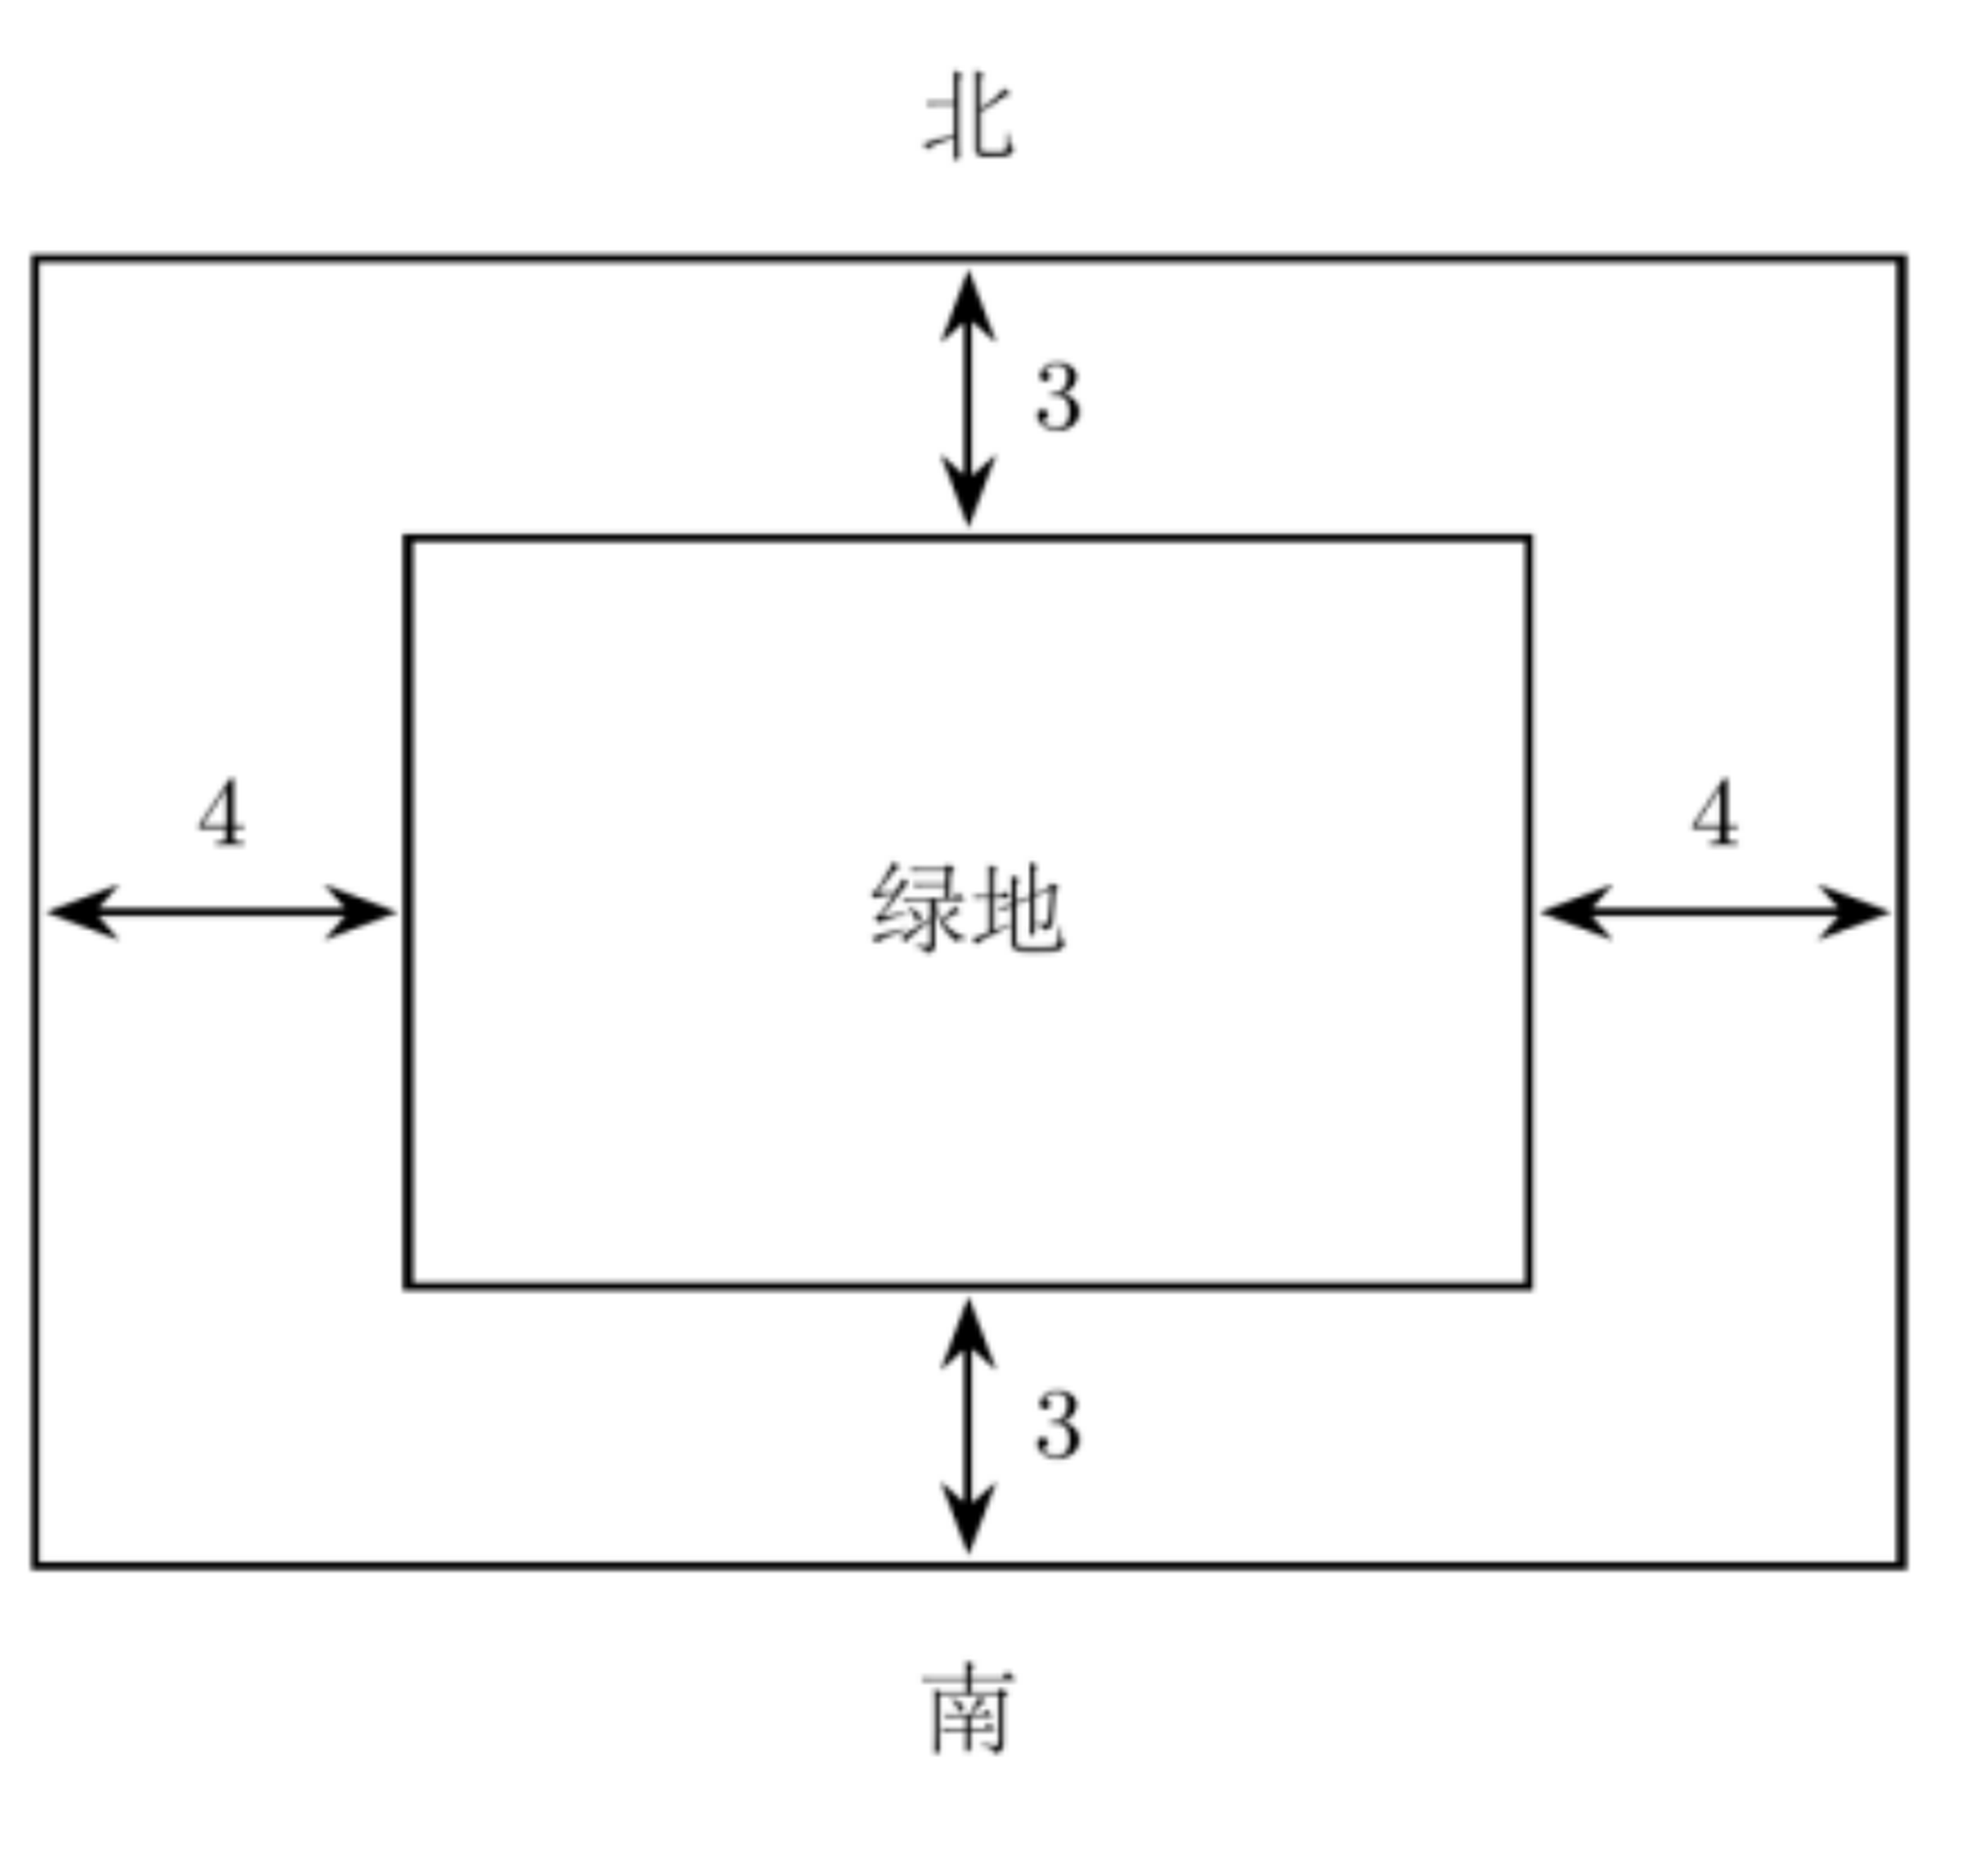
\includegraphics[width=0.32\textwidth]{figures/gao129_q19.png}
\end{center}

(1) 将 $S$ 表示为 $x$ 的函数；

(2) 试确定绿地东西方向的边长和南北方向的边长，使人行道的占地面积最小，并求出人行道的占地最小面积（结果精确到 0.1 米）

\ifanswer
\solbegin
\step{(1) 绿地南北方向的边长为 $\dfrac{1000}{x}$ 米，$x>0$.}
\step{外矩形东西、南北方向的边长分别为 $x+8$ 米、$\dfrac{1000}{x}+6$ 米.}
\step{因此 $S=(x+8)\left(\dfrac{1000}{x}+6\right)-1000=6x+\dfrac{8000}{x}+48, x>0$.}
\step{(2) 因为 $x>0,S=6x+\dfrac{8000}{x}+48\geqslant2\sqrt{6x\cdot\dfrac{8000}{x}}+48=48+80\sqrt{30}$.}
\step{等号当且仅当 $6x=\dfrac{8000}{x}$，即 $x=\dfrac{20\sqrt{30}}{3}\approx36.5$ 时成立，}
\step{此时绿地南北方向的边长为 $\dfrac{1000}{x}=\dfrac{1000}{\dfrac{20\sqrt{30}}{3}}=5\sqrt{30}\approx27.4$（米），}
\step{所以绿地东西方向、南北方向的边长分别约为 36.5 米、27.4 米时，}
\step{人行道的占地面积最小，最小面积为 $S_{min}=48+80\sqrt{30}\approx486.2$ 平方米.}
\solend
\fi

\item 已知集合 $A=\{x\mid x^2-3x+2=0\},B=\{x\mid x^2-ax+a-1=0\}$，

$C=\{x\mid x^2+2(m+1)x+m^2-5=0\}$.

(1) 若 $A=B$，求实数 $a$ 的值；

(2) 若 $B=\{1\}$，求实数 $a$ 的值；

(3) 若 $A\cap C=C$，求实数 $m$ 的取值范围.

\ifanswer
\solbegin
\step{(1) $A=\{1,2\}$，且 $x^2-ax+a-1=(x-1)(x-a+1)$，所以 $B=\{1,a-1\}$，}
\step{因此 $A=B\Leftrightarrow a-1=2\Leftrightarrow a=3$.}
\step{(2) $B=\{1\}$ 表示原方程只有一个不同的实数根，}
\step{得 $a-1=1$，即 $a=2$.}
\step{当 $a=2$ 时，原方程为 $(x-1)^2=0$，符合题意.}
\step{(3) $A\cap C=C\Leftrightarrow C\subseteq\{1,2\}$，}
\step{方程的判别式为 $\Delta=[2(m+1)]^2-4(m^2-5)=8(m+3)$.}
\step{当 $m<-3$ 时，$\Delta<0, C=\varnothing$，满足条件.}
\step{当 $m=-3$ 时，原方程为 $(x-2)^2=0, C=\{2\}$，满足条件.}
\step{当 $m>-3$ 时，方程有两个不同的实数根，必须有 $C=\{1,2\}$，}
\step{由韦达定理，$\begin{cases}-2(m+1)=1+2=3\\m^2-5=1\cdot2=2\end{cases}$，}
\step{第一式得 $m=-\dfrac52$，但此时 $m^2-5=\dfrac54\neq2$，不合题意.}
\step{因此 $m$ 的取值范围为 $(-\infty,-3]$.}
\solend
\fi

\item 设函数 $f(x)=ax^2+(1-a)x+a-2(a\in\R)$.

(1) 若关于 $x$ 的不等式 $f(x)\leqslant0$ 的解集为 $\left[0,\dfrac12\right]$，求实数 $a$ 的值；

(2) 若不等式 $f(x)\geqslant-2$ 对于实数 $a\in[-1,1]$ 时恒成立，求 $x$ 的取值范围；

(3) 解关于 $x$ 的不等式：$f(x)<a-1$.

\ifanswer
\solbegin
\step{(1) 由题意得 $0,\dfrac12$ 是方程 $ax^2+(1-a)x+a-2=0$ 的两个根，}
\step{则 $\begin{cases}0+\dfrac12=-\dfrac{1-a}{a}\\0\times\dfrac12=\dfrac{a-2}{a}\end{cases}\Rightarrow a=2$；}
\step{(2) $ax^2+(1-a)x+a-2\geqslant-2\Rightarrow a(x^2-x+1)+x\geqslant0$ 对 $a\in[-1,1]$ 恒成立，}
\step{则 $\begin{cases}-(x^2-x+1)+x\geqslant0\\(x^2-x+1)+x\geqslant0\end{cases}\Rightarrow\begin{cases}x=1\\x\in\R\end{cases}\Rightarrow x=1$，则 $x$ 的取值范围为 $\{1\}$；}
\step{(3) $f(x)<a-1$ 等价于 $ax^2+(1-a)x-1<0$，}
\step{当 $a=0$ 时，不等式可化为 $x<1$，解集为 $\{x\mid x<1\}$，}
\step{当 $a>0$ 时，不等式可化为 $(ax+1)(x-1)<0$，解集为 $\{x\mid -\dfrac1a<x<1\}$；}
\step{当 $a<0$ 时，不等式化为 $(ax+1)(x-1)<0$，}
\step{①当 $a=-1$ 时，$-\dfrac1a=1$，不等式的解集为 $\{x\mid x\neq1\}$；}
\step{②当 $-1<a<0$ 时，$-\dfrac1a>1$，不等式的解集为 $\{x\mid x<1$ 或 $x>-\dfrac1a\}$；}
\step{③当 $a<-1$ 时，$-\dfrac1a<1$，不等式的解集为 $\{x\mid x<-\dfrac1a$ 或 $x>1\}$；}
\step{综上，当 $a<-1$ 时，解集为 $\{x\mid x<-\dfrac1a$ 或 $x>1\}$；}
\step{当 $a=-1$ 时，解集为 $\{x\mid x\neq1\}$；}
\step{当 $-1<a<0$ 时，解集为 $\{x\mid x<1$ 或 $x>-\dfrac1a\}$；}
\step{当 $a=0$ 时，解集为 $\{x\mid x<1\}$；}
\step{当 $a>0$ 时，解集为 $\{x\mid -\dfrac1a<x<1\}$.}
\solend
\fi

\end{enumerate}

\end{document}
"
%
% 原始材料：微信公众号"魔都数学加油站"文章，作者破晓，2026-11-12 18:56 发布；
% 连载"27学年高一129"，原文标题"27学年高一129——2026-2027年上海市立达中学高一上期中"；
% 原文链接：https://mp.weixin.qq.com/s/gJhGsOBiWi7gW62u8EWLYA。
% 正文为 8 张 PNG 页（01、02、03、05、06 为 4762x6735，04、07、08 为 2560x3620），
% 题目下印有【解析】或【答案】，为讲评版。题目、解析均据原图转录；
% 卷面粉红色水印"魔都数学加油站"及公众号页脚未录入。全卷仅第 19 题有 1 幅插图。
%
% 卷首标题：原卷印作"2026-2027 年立达中学高一上期中"（公众号标题中的"上海市"
% 卷面标题行没有，本稿照卷面），年份区间按全稿惯例排 en dash；原卷未印副标题，
% 本卷为期中卷、跨集合与常用逻辑用语／不等式／函数三章，按题目内容标为
% "集合与常用逻辑用语、不等式、函数"（与 125、126 同为期中卷，口径相同）：
% 集合与逻辑见 Q3、Q4、Q13、Q20，不等式见 Q5、Q6、Q7、Q9、Q10、Q11、Q12、
% Q14、Q15、Q16、Q17、Q18、Q21，函数（含二次函数、基本不等式应用）见 Q8、Q19、Q21。
%
% 与原卷的排版差异：
%   ① 原文从第 3 题起，填空题编号为 3—12、选择题为 13—16、解答题为 17—21，本稿保留原题号；
%   ② 原卷每题下直接印【解析】／【答案】，本稿按全稿惯例置于答案版；第 3、5 题只印
%      【答案】，另提 \ans{}；第 13—16 题答案均在【解析】末句"故选 …"，题干括号内留空、
%      不另提 \ans{}；四道选择题括号内原卷均未印答案；
%   ③ 原卷未印副标题，本稿按"知识模块"口径补出（见上"卷首标题"）；
%   ④ 原卷填空横线按全稿惯例排为 \blankline[4.4em]；选择题括号排 \mbox{（\quad）}、
%      选项段前按惯例加 \keepwithprev；解答题不留作答区（原卷为讲评版，与 109—128 同）；
%   ⑤ 原卷数集排斜体 $R$，按全稿惯例改 \R；绝对值排 \lvert…\rvert，集合描述竖线排 \mid；
%      不等号按全稿惯例排 \leqslant／\geqslant；子题标号原卷一律用半角括号 (1)(2)(3)，本稿照录；
%   ⑥ 原卷第 19 题插图浮排在 Q18 解析右侧、"19."题干之上，本稿按体例就近置于 Q19
%      题干"如图所示"之后（居中 \includegraphics），图取原卷截图去水印；题前按惯例加
%      \needvspace{7cm} 守卫（照 高一120／127 成例），保证"题干 + 图"整块不被页边界切开；
%   ⑦ 原卷 Q8 解析续头印在第 2 页页首、Q17 解析续头印在第 5 页页首、Q19 题干续在第 6 页、
%      Q20 解析跨 6—7 页、Q21 解析续头印在第 8 页页首，本稿按题合并连续排版；
%      末页第 8 页为 Q21 解析的续尾，按实际印刷行单列（照 高一127 第 09 页续尾成例）。
%
% 判别式字形：第 8 题解析 $\Delta=m^2+4m>0$、第 10 题解析 $\Delta=k^2+6k=k(k+6)<0$、
%   第 20 题 (3) 解析 $\Delta=[2(m+1)]^2-4(m^2-5)=8(m+3)$ 三处原卷均排 $\Delta$
%   （等腰、高；回原图逐处放大核对、三处字形一致），照录 \Delta；全卷未出现 \triangle
%   （等边、扁）。
%
% 子集符号：第 13 题 ② $\{0,1,2\}\subseteq\{2,1,0\}$、③ $\varnothing\subseteq\{0,1,2\}$，
%   第 17 题 (2)② $B\subseteq A$、$B\subseteq(3,+\infty)$，第 20 题 (3) $C\subseteq\{1,2\}$
%   均印带下划线，照录 \subseteq；全卷未出现单线 \subset（回原图放大逐处确认）。
%
% 原卷存疑照录：
%   第 15 题解析"即 $m=4$，$n=3$ 时取等号"与题干 $\dfrac1m+n=1$、等号条件
%     $mn=\dfrac9{mn}$ 均不一致（按题应为 $n=\dfrac34$），照录、未统一；
%   第 18 题 (1) 题干"设 $M=2x^2+3x-1,N=7x-3$ 比较 $M$ 与 $N$ 两个数的大小"
%     两式间用半角逗号、且"$N=7x-3$"后无标点直接接"比较"，照录；
%   第 11 题解析"$1-x+2x-1=-(3x-2), 4x=2, x=\dfrac12$"、第 14 题解析
%     "$a=2, b=1, c=4, d=0$"、第 19 题解析"$6x+\dfrac{8000}{x}+48, x>0$"、
%     第 20 题解析"$\Delta<0, C=\varnothing$"与"$(x-2)^2=0, C=\{2\}$"、
%     第 12 题解析"$(x+y)^2=3+t\geqslant0,(x-y)^2=3-3t\geqslant0$"等处数学式内
%     用半角逗号，照录；
%   第 19 题题干"如图所示（图中单位：米）设绿地东西方向的边长为 $x$"在右括号后
%     无标点直接续"设"，照录；
%   第 21 题 (3) 解析先按 $a>0$、$a=0$、$a<0$ 分述解集，又在"综上"处重列全部
%     五类（含已给出的 $a>0$、$a=0$），照录；
%   第 21 题 (2) 题干与解析均作 $f(x)\geqslant-2$（与 $a(x^2-x+1)+x\geqslant0$ 相符），
%     照录，勿误读为 $f(x)\geqslant2$。
%
% 行数复核：逐题数 \step 条数，合计 93 条（Q3：0；Q4：2；Q5：0；Q6：3；Q7：3；
% Q8：2；Q9：4；Q10：3；Q11：5；Q12：5；Q13：1；Q14：3；Q15：3；Q16：7；
% Q17：7；Q18：8；Q19：8；Q20：13；Q21：16），与原卷印刷行逐题相等
% （cases 块作一个印刷行计）。第 3、5 题只印【答案】，提 \ans{}，不计入 \step 账；
% 四道选择题答案均在解析末句，括号内留空、不另提 \ans{}。
%
\documentclass[a4paper,11pt]{article}
\usepackage{common}

\begin{document}

\examtitlest[3]{2026--2027 年立达中学高一上期中}{集合与常用逻辑用语、不等式、函数}

\bigsec{一、填空题}

\begin{enumerate}
\setcounter{enumi}{2}

\item 若 $A=\{x\mid -3<x\leqslant2\},B=\{x\mid 1<x\leqslant3\}$，则 $A\cup B=$\blankline[4.4em].

\ifanswer
\ans{$(-3,3]$}
\fi

\item 若 $A$ 是 $B$ 的必要非充分条件，$B$ 是 $C$ 的充要条件，$C$ 是 $D$ 的必要非充分条件，则 $D$ 是 $A$ 的\blankline[4.4em]条件.

\ifanswer
\solbegin
\step{$D\Rightarrow C\Leftrightarrow B\Rightarrow A$，且 $A\nRightarrow B$，因此 $D\Rightarrow A$ 且 $A\nRightarrow D$，}
\step{故 $D$ 是 $A$ 的充分非必要条件.}
\solend
\fi

\item 不等式 $\dfrac1x<1$ 的解集为\blankline[4.4em].

\ifanswer
\ans{$(-\infty,0)\cup(1,+\infty)$}
\fi

\item 已知正实数 $x$、$y$ 满足 $2x+y=2$，则 $xy$ 的最大值为\blankline[4.4em].

\ifanswer
\solbegin
\step{因为 $x>0$，$y>0$，所以 $2x+y\geqslant2\sqrt{2xy}$（当且仅当 $2x=y$ 时，取等号），}
\step{又因为 $2x+y=2$，所以 $2\geqslant2\sqrt{2xy}$（当且仅当 $2x=y$ 时，取等号），}
\step{即 $xy\leqslant\dfrac12$，则 $xy$ 的最大值为 $\dfrac12$.}
\solend
\fi

\item 已知 $x\in\R$，函数 $y=\lvert x+2\rvert+\lvert x-3\rvert$ 的最小值为\blankline[4.4em].

\ifanswer
\solbegin
\step{由 $\lvert x+2\rvert+\lvert x-3\rvert\geqslant\lvert(x+2)-(x-3)\rvert=5$，}
\step{当且仅当 $(x+2)(x-3)\leqslant0$，即 $-2\leqslant x\leqslant3$ 时，上式取等号，}
\step{则函数 $y=\lvert x+2\rvert+\lvert x-3\rvert$ 的最小值是 5.}
\solend
\fi

\item 已知实系数一元二次方程 $x^2+mx-m=0$ 的两根分别为 $x_1,x_2$，且 $\lvert x_1-x_2\rvert=\sqrt{21}$，实数 $m$ 的值为\blankline[4.4em].

\ifanswer
\solbegin
\step{由题意得 $\Delta=m^2+4m>0$，解得 $m>0$ 或 $m<-4,x_1+x_2=-m,x_1x_2=-m$，}
\step{则 $\lvert x_1-x_2\rvert=\sqrt{(x_1+x_2)^2-4x_1x_2}=\sqrt{m^2+4m}=\sqrt{21}$，解得 $m=-7$ 或 $3$.}
\solend
\fi

\item 已知不等式 $ax^2-5x+b>0$ 的解集是 $\{x\mid -3<x<-2\}$，则不等式 $bx^2-5x+a>0$ 的解集是\blankline[4.4em].

\ifanswer
\solbegin
\step{$ax^2-5x+b=a(x+3)(x+2)$，比较系数得 $5a=-5,b=6a$，}
\step{即 $a=-1,b=-6$.}
\step{$bx^2-5x+a>0\Leftrightarrow(3x+1)(2x+1)<0\Leftrightarrow-\dfrac12<x<-\dfrac13$，}
\step{故解集为 $\left\{x\mid -\dfrac12<x<-\dfrac13\right\}$.}
\solend
\fi

\item 不等式 $4kx^2+kx-\dfrac38<0$ 对于一切实数 $x$ 都成立，则实数 $k$ 的取值范围是\blankline[4.4em].

\ifanswer
\solbegin
\step{$k=0$ 时，不等式恒成立；}
\step{$k\neq0$ 时，须 $4k<0$ 且 $\Delta=k^2+6k=k(k+6)<0$，解得 $-6<k<0$.}
\step{因此 $k\in(-6,0]$.}
\solend
\fi

\item 设 $x\in\R$，方程 $\lvert 1-x\rvert+\lvert 2x-1\rvert=\lvert 3x-2\rvert$ 的解集为\blankline[4.4em].

\ifanswer
\solbegin
\step{当 $x\leqslant\dfrac12$ 时，方程化为 $1-x-(2x-1)=-(3x-2)$，$2-3x=-3x+2$，恒成立，}
\step{当 $\dfrac12<x\leqslant\dfrac23$ 时，方程化为 $1-x+2x-1=-(3x-2), 4x=2, x=\dfrac12$，不合题意，}
\step{当 $\dfrac23<x\leqslant1$ 时，方程化为 $1-x+2x-1=3x-2$，$2x=2$，解得 $x=1$，}
\step{当 $x>1$ 时，方程化为 $-(1-x)+2x-1=3x-2$，$3x-2=3x-2$，恒成立，}
\step{综上所述，$\lvert 1-x\rvert+\lvert 2x-1\rvert=\lvert 3x-2\rvert$ 的解集为 $\left(-\infty,\dfrac12\right]\cup[1,+\infty)$.}
\solend
\fi

\item 已知非零实数 $x,y$ 满足 $x^2+xy+y^2=3$，则 $x^2-xy+y^2$ 的取值范围是\blankline[4.4em].

\ifanswer
\solbegin
\step{令 $t=xy\neq0$，由 $(x+y)^2=3+t\geqslant0,(x-y)^2=3-3t\geqslant0$，}
\step{得 $t\in[-3,0)\cup(0,1]$.}
\step{对上述任意 $t$，联立 $x+y=\sqrt{3+t},x-y=\sqrt{3-3t}$，所得 $x,y$ 满足原条件，}
\step{因此上述 $t$ 均可取到.}
\step{于是 $x^2-xy+y^2=3-2t$ 的取值范围为 $[1,3)\cup(3,9]$.}
\solend
\fi

\end{enumerate}

\bigsec{二、选择题}

\begin{enumerate}
\setcounter{enumi}{12}

\item 下列各式中，正确的个数是\mbox{（\quad）}

① $\{0\}\in\{0,1,2\}$；② $\{0,1,2\}\subseteq\{2,1,0\}$；③ $\varnothing\subseteq\{0,1,2\}$；④ $\varnothing=\{0\}$；⑤ $\{0,1\}=\{(0,1)\}$；

⑥ $0=\{0\}$.

\keepwithprev
A. $1$\qquad\qquad B. $2$\qquad\qquad C. $3$\qquad\qquad D. $4$

\ifanswer
\solbegin
\step{①不正确，②正确，③正确，④不正确，⑤不正确，⑥不正确. 故选 $B$.}
\solend
\fi

\item 下列四个命题中，为真命题的是\mbox{（\quad）}

\keepwithprev
A. 若 $a>b$，则 $ac^2>bc^2$\qquad\qquad B. 若 $a>b,c>d$，则 $a-c>b-d$

C. 若 $ac^2>bc^2$，则 $a>b$\qquad\qquad D. 若 $a>b$，则 $\dfrac1a<\dfrac1b$

\ifanswer
\solbegin
\step{C 中，$(a-b)c^2>0$，必有 $c^2>0$ 且 $a-b>0$，即 $a>b$.}
\step{A 取 $c=0$；B 取 $a=2, b=1, c=4, d=0$；D 取 $a=1, b=-1$，均不成立.}
\step{故选 $C$.}
\solend
\fi

\item 已知 $m$、$n\in(0,+\infty)$，$\dfrac1m+n=1$，则 $m+\dfrac9n$ 的最小值为\mbox{（\quad）}

\keepwithprev
A. $13$\qquad\qquad B. $16$\qquad\qquad C. $3$\qquad\qquad D. $6$

\ifanswer
\solbegin
\step{因为 $m$、$n\in(0,+\infty)$，$\dfrac1m+n=1$，}
\step{所以 $m+\dfrac9n=(m+\dfrac9n)(\dfrac1m+n)=10+mn+\dfrac9{mn}\geqslant10+2\sqrt{mn\cdot\dfrac9{mn}}=16$，}
\step{当且仅当 $mn=\dfrac9{mn}$，即 $m=4$，$n=3$ 时取等号. 故选 $B$.}
\solend
\fi

\item 下列不等式：① $\left\lvert x+\dfrac1x\right\rvert\geqslant2$；② $x^2+2x+1>0$；③ $\lvert x\rvert+\lvert x-1\rvert\geqslant1$；④ $\dfrac{x}{x^2+x+1}<1$；

解集为 $\R$ 的不等式的个数是\mbox{（\quad）}

\keepwithprev
A. $0$\qquad\qquad B. $1$\qquad\qquad C. $2$\qquad\qquad D. $3$

\ifanswer
\solbegin
\step{对于①，当 $x=0$ 时，$\dfrac1x$ 无意义，故 $\left\lvert x+\dfrac1x\right\rvert\geqslant2$ 的解集不是 $\R$，错误；}
\step{对于②，$x^2+2x+1=(x+1)^2\geqslant0$，当 $x=-1$ 取到等号，解集不是 $\R$，故错误；}
\step{对于③，$\lvert x\rvert+\lvert x-1\rvert\geqslant\lvert x-(x-1)\rvert=1$，当 $x(x-1)\leqslant0$ 时取等号，解集为 $\R$，}
\step{故正确；}
\step{对于④，由于 $x^2+x+1>0$ 恒成立，}
\step{故 $\dfrac{x}{x^2+x+1}<1$ 等价于 $x<x^2+x+1\Rightarrow x^2+1>0$ 恒成立，故解集为 $\R$，正确，}
\step{故正确的有③④，故选 $C$.}
\solend
\fi

\end{enumerate}

\bigsec{三、解答题}

\begin{enumerate}
\setcounter{enumi}{16}

\item (1) 解不等式组 $\begin{cases}\dfrac{x+3}{x+1}\leqslant2\\\lvert 2x-3\rvert\leqslant2\end{cases}$.

(2) 已知集合 $A=\{x\mid -x+3<0\},B=\{x\mid a\leqslant x\leqslant a+3\}$.

①当 $a=2$，求集合 $A\cap B$；

②若 $A\cup B=A$，求实数 $a$ 的取值范围.

\ifanswer
\solbegin
\step{(1) 由 $\begin{cases}\dfrac{x+3}{x+1}\leqslant2\\\lvert 2x-3\rvert\leqslant2\end{cases}$ 得 $\begin{cases}\dfrac{x+3-2x-2}{x+1}\leqslant0\\-2\leqslant2x-3\leqslant2\end{cases}$，即 $\begin{cases}\dfrac{-x+1}{x+1}\leqslant0\\1\leqslant2x\leqslant5\end{cases}$，则 $\begin{cases}\dfrac{x-1}{x+1}\geqslant0\\\dfrac12\leqslant x\leqslant\dfrac52\end{cases}$，}
\step{解得 $1\leqslant x\leqslant\dfrac52$，即原不等式组的解集为 $\left[1,\dfrac52\right]$.}
\step{(2) $-x+3<0\Leftrightarrow x>3$，所以 $A=(3,+\infty)$.}
\step{①当 $a=2$ 时，$B=[2,5], A\cap B=(3,+\infty)\cap[2,5]=(3,5]$.}
\step{②$A\cup B=A\Leftrightarrow B\subseteq A$.}
\step{因为 $B=[a,a+3]$，且左端点 $a\in B$，所以 $B\subseteq(3,+\infty)\Leftrightarrow a>3$，}
\step{实数 $a$ 的取值范围为 $(3,+\infty)$.}
\solend
\fi

\item (1) 设 $M=2x^2+3x-1,N=7x-3$ 比较 $M$ 与 $N$ 两个数的大小.

(2) 解关于 $x$ 的不等式：$x^2-(a+3)x+3a<0$，$a\in\R$.

\ifanswer
\solbegin
\step{(1) $M-N=2x^2+3x-1-(7x-3)=2(x-1)^2$.}
\step{$x=1$ 时，$M-N=0$，即 $M=N$.}
\step{$x\neq1$ 时，$M-N>0$，即 $M>N$.}
\step{(2) 不等式 $x^2-(a+3)x+3a<0$ 可化为 $(x-3)(x-a)<0$，}
\step{不等式对应方程的解为 $a$ 和 3，}
\step{当 $a<3$ 时，不等式 $x^2-(a+3)x+3a<0$ 的解集为 $(a,3)$，}
\step{当 $a=3$ 时，不等式 $x^2-(a+3)x+3a<0$ 的解集为 $\varnothing$，}
\step{当 $a>3$ 时，不等式 $x^2-(a+3)x+3a<0$ 的解集为 $(3,a)$.}
\solend
\fi

% 第 19 题是"题干 + 图"约 7cm 的一整块，答案版实测断点落在题干之后（图被推到次页页首），
% 照 高一120／127 成例在题前先量一次页高，不够就把"题干 + 图"整块一起挪到次页。
\needvspace{7cm}
\item 某新建居民小区欲建一面积为 1000 平方米的矩形绿地，在绿地四周铺设人行道，设计要求绿地南北两侧人行道宽 3 米，东西两侧人行道宽 4 米，如图所示（图中单位：米）设绿地东西方向的边长为 $x$，人行道的占地面积为 $S$.

\begin{center}
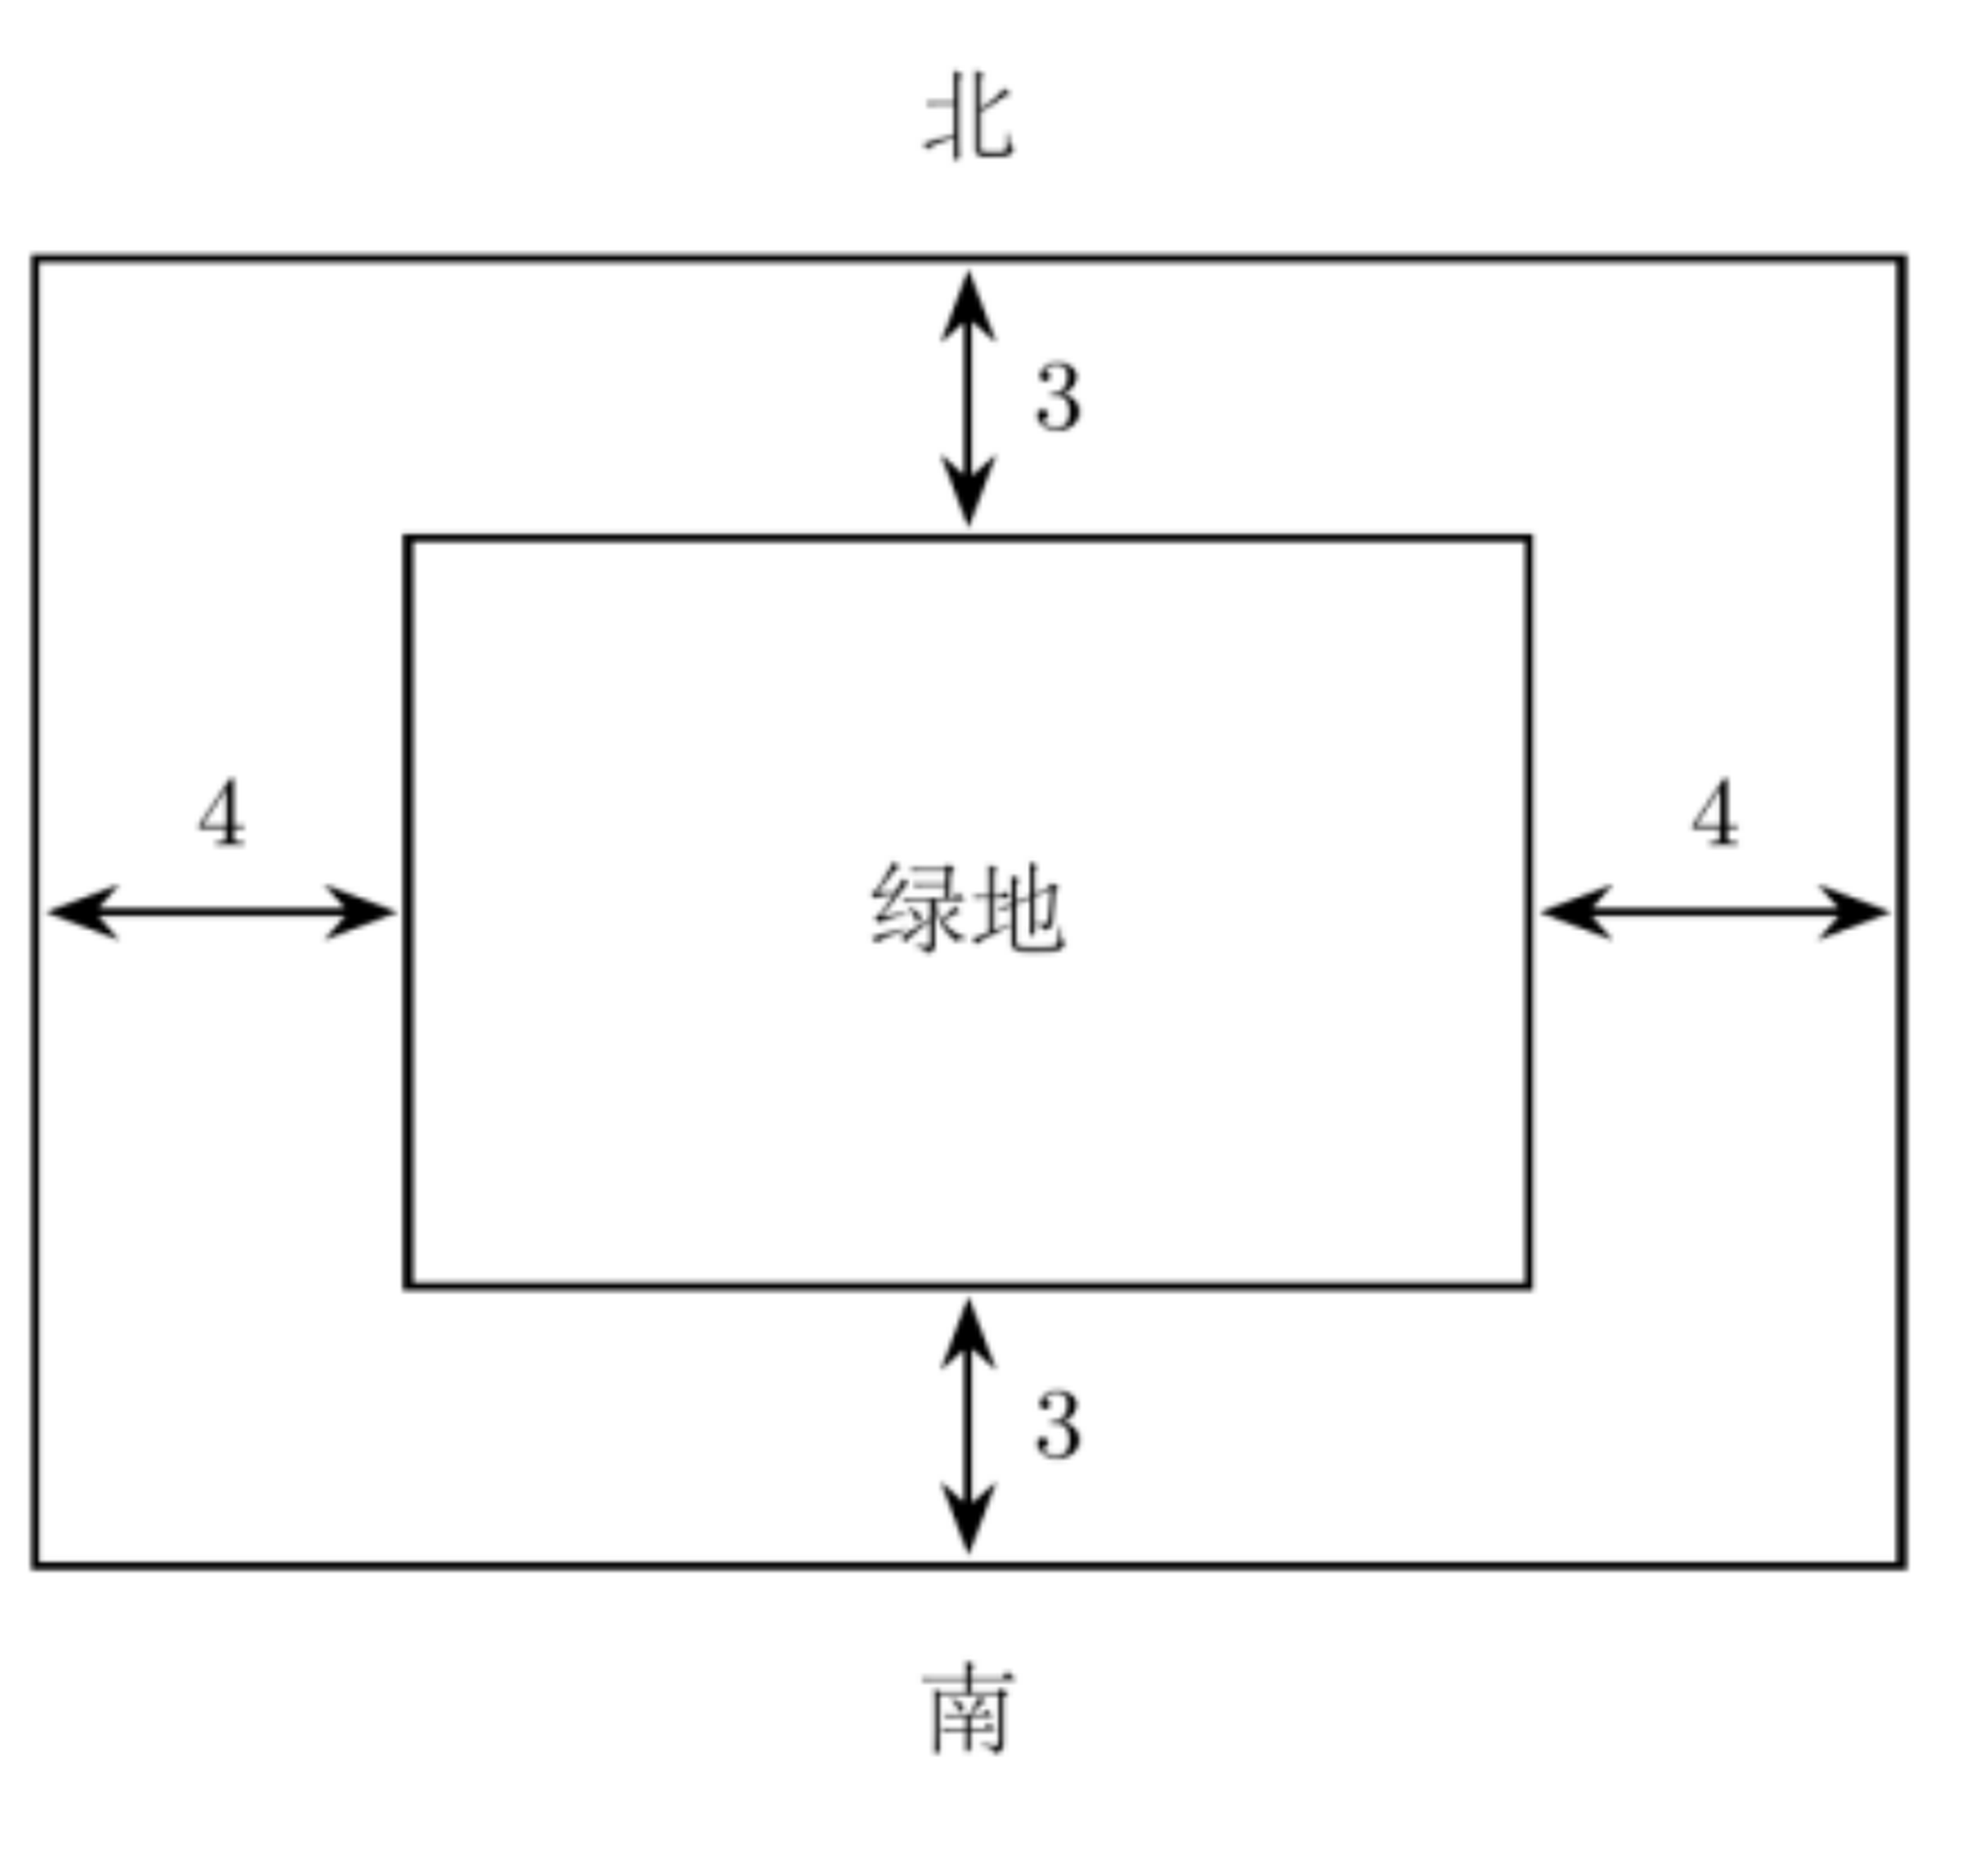
\includegraphics[width=0.32\textwidth]{figures/gao129_q19.png}
\end{center}

(1) 将 $S$ 表示为 $x$ 的函数；

(2) 试确定绿地东西方向的边长和南北方向的边长，使人行道的占地面积最小，并求出人行道的占地最小面积（结果精确到 0.1 米）

\ifanswer
\solbegin
\step{(1) 绿地南北方向的边长为 $\dfrac{1000}{x}$ 米，$x>0$.}
\step{外矩形东西、南北方向的边长分别为 $x+8$ 米、$\dfrac{1000}{x}+6$ 米.}
\step{因此 $S=(x+8)\left(\dfrac{1000}{x}+6\right)-1000=6x+\dfrac{8000}{x}+48, x>0$.}
\step{(2) 因为 $x>0,S=6x+\dfrac{8000}{x}+48\geqslant2\sqrt{6x\cdot\dfrac{8000}{x}}+48=48+80\sqrt{30}$.}
\step{等号当且仅当 $6x=\dfrac{8000}{x}$，即 $x=\dfrac{20\sqrt{30}}{3}\approx36.5$ 时成立，}
\step{此时绿地南北方向的边长为 $\dfrac{1000}{x}=\dfrac{1000}{\dfrac{20\sqrt{30}}{3}}=5\sqrt{30}\approx27.4$（米），}
\step{所以绿地东西方向、南北方向的边长分别约为 36.5 米、27.4 米时，}
\step{人行道的占地面积最小，最小面积为 $S_{min}=48+80\sqrt{30}\approx486.2$ 平方米.}
\solend
\fi

\item 已知集合 $A=\{x\mid x^2-3x+2=0\},B=\{x\mid x^2-ax+a-1=0\}$，

$C=\{x\mid x^2+2(m+1)x+m^2-5=0\}$.

(1) 若 $A=B$，求实数 $a$ 的值；

(2) 若 $B=\{1\}$，求实数 $a$ 的值；

(3) 若 $A\cap C=C$，求实数 $m$ 的取值范围.

\ifanswer
\solbegin
\step{(1) $A=\{1,2\}$，且 $x^2-ax+a-1=(x-1)(x-a+1)$，所以 $B=\{1,a-1\}$，}
\step{因此 $A=B\Leftrightarrow a-1=2\Leftrightarrow a=3$.}
\step{(2) $B=\{1\}$ 表示原方程只有一个不同的实数根，}
\step{得 $a-1=1$，即 $a=2$.}
\step{当 $a=2$ 时，原方程为 $(x-1)^2=0$，符合题意.}
\step{(3) $A\cap C=C\Leftrightarrow C\subseteq\{1,2\}$，}
\step{方程的判别式为 $\Delta=[2(m+1)]^2-4(m^2-5)=8(m+3)$.}
\step{当 $m<-3$ 时，$\Delta<0, C=\varnothing$，满足条件.}
\step{当 $m=-3$ 时，原方程为 $(x-2)^2=0, C=\{2\}$，满足条件.}
\step{当 $m>-3$ 时，方程有两个不同的实数根，必须有 $C=\{1,2\}$，}
\step{由韦达定理，$\begin{cases}-2(m+1)=1+2=3\\m^2-5=1\cdot2=2\end{cases}$，}
\step{第一式得 $m=-\dfrac52$，但此时 $m^2-5=\dfrac54\neq2$，不合题意.}
\step{因此 $m$ 的取值范围为 $(-\infty,-3]$.}
\solend
\fi

\item 设函数 $f(x)=ax^2+(1-a)x+a-2(a\in\R)$.

(1) 若关于 $x$ 的不等式 $f(x)\leqslant0$ 的解集为 $\left[0,\dfrac12\right]$，求实数 $a$ 的值；

(2) 若不等式 $f(x)\geqslant-2$ 对于实数 $a\in[-1,1]$ 时恒成立，求 $x$ 的取值范围；

(3) 解关于 $x$ 的不等式：$f(x)<a-1$.

\ifanswer
\solbegin
\step{(1) 由题意得 $0,\dfrac12$ 是方程 $ax^2+(1-a)x+a-2=0$ 的两个根，}
\step{则 $\begin{cases}0+\dfrac12=-\dfrac{1-a}{a}\\0\times\dfrac12=\dfrac{a-2}{a}\end{cases}\Rightarrow a=2$；}
\step{(2) $ax^2+(1-a)x+a-2\geqslant-2\Rightarrow a(x^2-x+1)+x\geqslant0$ 对 $a\in[-1,1]$ 恒成立，}
\step{则 $\begin{cases}-(x^2-x+1)+x\geqslant0\\(x^2-x+1)+x\geqslant0\end{cases}\Rightarrow\begin{cases}x=1\\x\in\R\end{cases}\Rightarrow x=1$，则 $x$ 的取值范围为 $\{1\}$；}
\step{(3) $f(x)<a-1$ 等价于 $ax^2+(1-a)x-1<0$，}
\step{当 $a=0$ 时，不等式可化为 $x<1$，解集为 $\{x\mid x<1\}$，}
\step{当 $a>0$ 时，不等式可化为 $(ax+1)(x-1)<0$，解集为 $\{x\mid -\dfrac1a<x<1\}$；}
\step{当 $a<0$ 时，不等式化为 $(ax+1)(x-1)<0$，}
\step{①当 $a=-1$ 时，$-\dfrac1a=1$，不等式的解集为 $\{x\mid x\neq1\}$；}
\step{②当 $-1<a<0$ 时，$-\dfrac1a>1$，不等式的解集为 $\{x\mid x<1$ 或 $x>-\dfrac1a\}$；}
\step{③当 $a<-1$ 时，$-\dfrac1a<1$，不等式的解集为 $\{x\mid x<-\dfrac1a$ 或 $x>1\}$；}
\step{综上，当 $a<-1$ 时，解集为 $\{x\mid x<-\dfrac1a$ 或 $x>1\}$；}
\step{当 $a=-1$ 时，解集为 $\{x\mid x\neq1\}$；}
\step{当 $-1<a<0$ 时，解集为 $\{x\mid x<1$ 或 $x>-\dfrac1a\}$；}
\step{当 $a=0$ 时，解集为 $\{x\mid x<1\}$；}
\step{当 $a>0$ 时，解集为 $\{x\mid -\dfrac1a<x<1\}$.}
\solend
\fi

\end{enumerate}

\end{document}
"
% 紧凑版：xelatex "\def\iscompact{1}% 高一129_立达中学_期中.tex
%   —— 高一上数学"2026-2027 年立达中学高一上期中"（试卷版/答案版）
% 试卷版：xelatex 高一129_立达中学_期中.tex
% 答案版：xelatex "\def\isanswer{1}% 高一129_立达中学_期中.tex
%   —— 高一上数学"2026-2027 年立达中学高一上期中"（试卷版/答案版）
% 试卷版：xelatex 高一129_立达中学_期中.tex
% 答案版：xelatex "\def\isanswer{1}\input{高一129_立达中学_期中.tex}"
% 紧凑版：xelatex "\def\iscompact{1}\input{高一129_立达中学_期中.tex}"
%
% 原始材料：微信公众号"魔都数学加油站"文章，作者破晓，2026-11-12 18:56 发布；
% 连载"27学年高一129"，原文标题"27学年高一129——2026-2027年上海市立达中学高一上期中"；
% 原文链接：https://mp.weixin.qq.com/s/gJhGsOBiWi7gW62u8EWLYA。
% 正文为 8 张 PNG 页（01、02、03、05、06 为 4762x6735，04、07、08 为 2560x3620），
% 题目下印有【解析】或【答案】，为讲评版。题目、解析均据原图转录；
% 卷面粉红色水印"魔都数学加油站"及公众号页脚未录入。全卷仅第 19 题有 1 幅插图。
%
% 卷首标题：原卷印作"2026-2027 年立达中学高一上期中"（公众号标题中的"上海市"
% 卷面标题行没有，本稿照卷面），年份区间按全稿惯例排 en dash；原卷未印副标题，
% 本卷为期中卷、跨集合与常用逻辑用语／不等式／函数三章，按题目内容标为
% "集合与常用逻辑用语、不等式、函数"（与 125、126 同为期中卷，口径相同）：
% 集合与逻辑见 Q3、Q4、Q13、Q20，不等式见 Q5、Q6、Q7、Q9、Q10、Q11、Q12、
% Q14、Q15、Q16、Q17、Q18、Q21，函数（含二次函数、基本不等式应用）见 Q8、Q19、Q21。
%
% 与原卷的排版差异：
%   ① 原文从第 3 题起，填空题编号为 3—12、选择题为 13—16、解答题为 17—21，本稿保留原题号；
%   ② 原卷每题下直接印【解析】／【答案】，本稿按全稿惯例置于答案版；第 3、5 题只印
%      【答案】，另提 \ans{}；第 13—16 题答案均在【解析】末句"故选 …"，题干括号内留空、
%      不另提 \ans{}；四道选择题括号内原卷均未印答案；
%   ③ 原卷未印副标题，本稿按"知识模块"口径补出（见上"卷首标题"）；
%   ④ 原卷填空横线按全稿惯例排为 \blankline[4.4em]；选择题括号排 \mbox{（\quad）}、
%      选项段前按惯例加 \keepwithprev；解答题不留作答区（原卷为讲评版，与 109—128 同）；
%   ⑤ 原卷数集排斜体 $R$，按全稿惯例改 \R；绝对值排 \lvert…\rvert，集合描述竖线排 \mid；
%      不等号按全稿惯例排 \leqslant／\geqslant；子题标号原卷一律用半角括号 (1)(2)(3)，本稿照录；
%   ⑥ 原卷第 19 题插图浮排在 Q18 解析右侧、"19."题干之上，本稿按体例就近置于 Q19
%      题干"如图所示"之后（居中 \includegraphics），图取原卷截图去水印；题前按惯例加
%      \needvspace{7cm} 守卫（照 高一120／127 成例），保证"题干 + 图"整块不被页边界切开；
%   ⑦ 原卷 Q8 解析续头印在第 2 页页首、Q17 解析续头印在第 5 页页首、Q19 题干续在第 6 页、
%      Q20 解析跨 6—7 页、Q21 解析续头印在第 8 页页首，本稿按题合并连续排版；
%      末页第 8 页为 Q21 解析的续尾，按实际印刷行单列（照 高一127 第 09 页续尾成例）。
%
% 判别式字形：第 8 题解析 $\Delta=m^2+4m>0$、第 10 题解析 $\Delta=k^2+6k=k(k+6)<0$、
%   第 20 题 (3) 解析 $\Delta=[2(m+1)]^2-4(m^2-5)=8(m+3)$ 三处原卷均排 $\Delta$
%   （等腰、高；回原图逐处放大核对、三处字形一致），照录 \Delta；全卷未出现 \triangle
%   （等边、扁）。
%
% 子集符号：第 13 题 ② $\{0,1,2\}\subseteq\{2,1,0\}$、③ $\varnothing\subseteq\{0,1,2\}$，
%   第 17 题 (2)② $B\subseteq A$、$B\subseteq(3,+\infty)$，第 20 题 (3) $C\subseteq\{1,2\}$
%   均印带下划线，照录 \subseteq；全卷未出现单线 \subset（回原图放大逐处确认）。
%
% 原卷存疑照录：
%   第 15 题解析"即 $m=4$，$n=3$ 时取等号"与题干 $\dfrac1m+n=1$、等号条件
%     $mn=\dfrac9{mn}$ 均不一致（按题应为 $n=\dfrac34$），照录、未统一；
%   第 18 题 (1) 题干"设 $M=2x^2+3x-1,N=7x-3$ 比较 $M$ 与 $N$ 两个数的大小"
%     两式间用半角逗号、且"$N=7x-3$"后无标点直接接"比较"，照录；
%   第 11 题解析"$1-x+2x-1=-(3x-2), 4x=2, x=\dfrac12$"、第 14 题解析
%     "$a=2, b=1, c=4, d=0$"、第 19 题解析"$6x+\dfrac{8000}{x}+48, x>0$"、
%     第 20 题解析"$\Delta<0, C=\varnothing$"与"$(x-2)^2=0, C=\{2\}$"、
%     第 12 题解析"$(x+y)^2=3+t\geqslant0,(x-y)^2=3-3t\geqslant0$"等处数学式内
%     用半角逗号，照录；
%   第 19 题题干"如图所示（图中单位：米）设绿地东西方向的边长为 $x$"在右括号后
%     无标点直接续"设"，照录；
%   第 21 题 (3) 解析先按 $a>0$、$a=0$、$a<0$ 分述解集，又在"综上"处重列全部
%     五类（含已给出的 $a>0$、$a=0$），照录；
%   第 21 题 (2) 题干与解析均作 $f(x)\geqslant-2$（与 $a(x^2-x+1)+x\geqslant0$ 相符），
%     照录，勿误读为 $f(x)\geqslant2$。
%
% 行数复核：逐题数 \step 条数，合计 93 条（Q3：0；Q4：2；Q5：0；Q6：3；Q7：3；
% Q8：2；Q9：4；Q10：3；Q11：5；Q12：5；Q13：1；Q14：3；Q15：3；Q16：7；
% Q17：7；Q18：8；Q19：8；Q20：13；Q21：16），与原卷印刷行逐题相等
% （cases 块作一个印刷行计）。第 3、5 题只印【答案】，提 \ans{}，不计入 \step 账；
% 四道选择题答案均在解析末句，括号内留空、不另提 \ans{}。
%
\documentclass[a4paper,11pt]{article}
\usepackage{common}

\begin{document}

\examtitlest[3]{2026--2027 年立达中学高一上期中}{集合与常用逻辑用语、不等式、函数}

\bigsec{一、填空题}

\begin{enumerate}
\setcounter{enumi}{2}

\item 若 $A=\{x\mid -3<x\leqslant2\},B=\{x\mid 1<x\leqslant3\}$，则 $A\cup B=$\blankline[4.4em].

\ifanswer
\ans{$(-3,3]$}
\fi

\item 若 $A$ 是 $B$ 的必要非充分条件，$B$ 是 $C$ 的充要条件，$C$ 是 $D$ 的必要非充分条件，则 $D$ 是 $A$ 的\blankline[4.4em]条件.

\ifanswer
\solbegin
\step{$D\Rightarrow C\Leftrightarrow B\Rightarrow A$，且 $A\nRightarrow B$，因此 $D\Rightarrow A$ 且 $A\nRightarrow D$，}
\step{故 $D$ 是 $A$ 的充分非必要条件.}
\solend
\fi

\item 不等式 $\dfrac1x<1$ 的解集为\blankline[4.4em].

\ifanswer
\ans{$(-\infty,0)\cup(1,+\infty)$}
\fi

\item 已知正实数 $x$、$y$ 满足 $2x+y=2$，则 $xy$ 的最大值为\blankline[4.4em].

\ifanswer
\solbegin
\step{因为 $x>0$，$y>0$，所以 $2x+y\geqslant2\sqrt{2xy}$（当且仅当 $2x=y$ 时，取等号），}
\step{又因为 $2x+y=2$，所以 $2\geqslant2\sqrt{2xy}$（当且仅当 $2x=y$ 时，取等号），}
\step{即 $xy\leqslant\dfrac12$，则 $xy$ 的最大值为 $\dfrac12$.}
\solend
\fi

\item 已知 $x\in\R$，函数 $y=\lvert x+2\rvert+\lvert x-3\rvert$ 的最小值为\blankline[4.4em].

\ifanswer
\solbegin
\step{由 $\lvert x+2\rvert+\lvert x-3\rvert\geqslant\lvert(x+2)-(x-3)\rvert=5$，}
\step{当且仅当 $(x+2)(x-3)\leqslant0$，即 $-2\leqslant x\leqslant3$ 时，上式取等号，}
\step{则函数 $y=\lvert x+2\rvert+\lvert x-3\rvert$ 的最小值是 5.}
\solend
\fi

\item 已知实系数一元二次方程 $x^2+mx-m=0$ 的两根分别为 $x_1,x_2$，且 $\lvert x_1-x_2\rvert=\sqrt{21}$，实数 $m$ 的值为\blankline[4.4em].

\ifanswer
\solbegin
\step{由题意得 $\Delta=m^2+4m>0$，解得 $m>0$ 或 $m<-4,x_1+x_2=-m,x_1x_2=-m$，}
\step{则 $\lvert x_1-x_2\rvert=\sqrt{(x_1+x_2)^2-4x_1x_2}=\sqrt{m^2+4m}=\sqrt{21}$，解得 $m=-7$ 或 $3$.}
\solend
\fi

\item 已知不等式 $ax^2-5x+b>0$ 的解集是 $\{x\mid -3<x<-2\}$，则不等式 $bx^2-5x+a>0$ 的解集是\blankline[4.4em].

\ifanswer
\solbegin
\step{$ax^2-5x+b=a(x+3)(x+2)$，比较系数得 $5a=-5,b=6a$，}
\step{即 $a=-1,b=-6$.}
\step{$bx^2-5x+a>0\Leftrightarrow(3x+1)(2x+1)<0\Leftrightarrow-\dfrac12<x<-\dfrac13$，}
\step{故解集为 $\left\{x\mid -\dfrac12<x<-\dfrac13\right\}$.}
\solend
\fi

\item 不等式 $4kx^2+kx-\dfrac38<0$ 对于一切实数 $x$ 都成立，则实数 $k$ 的取值范围是\blankline[4.4em].

\ifanswer
\solbegin
\step{$k=0$ 时，不等式恒成立；}
\step{$k\neq0$ 时，须 $4k<0$ 且 $\Delta=k^2+6k=k(k+6)<0$，解得 $-6<k<0$.}
\step{因此 $k\in(-6,0]$.}
\solend
\fi

\item 设 $x\in\R$，方程 $\lvert 1-x\rvert+\lvert 2x-1\rvert=\lvert 3x-2\rvert$ 的解集为\blankline[4.4em].

\ifanswer
\solbegin
\step{当 $x\leqslant\dfrac12$ 时，方程化为 $1-x-(2x-1)=-(3x-2)$，$2-3x=-3x+2$，恒成立，}
\step{当 $\dfrac12<x\leqslant\dfrac23$ 时，方程化为 $1-x+2x-1=-(3x-2), 4x=2, x=\dfrac12$，不合题意，}
\step{当 $\dfrac23<x\leqslant1$ 时，方程化为 $1-x+2x-1=3x-2$，$2x=2$，解得 $x=1$，}
\step{当 $x>1$ 时，方程化为 $-(1-x)+2x-1=3x-2$，$3x-2=3x-2$，恒成立，}
\step{综上所述，$\lvert 1-x\rvert+\lvert 2x-1\rvert=\lvert 3x-2\rvert$ 的解集为 $\left(-\infty,\dfrac12\right]\cup[1,+\infty)$.}
\solend
\fi

\item 已知非零实数 $x,y$ 满足 $x^2+xy+y^2=3$，则 $x^2-xy+y^2$ 的取值范围是\blankline[4.4em].

\ifanswer
\solbegin
\step{令 $t=xy\neq0$，由 $(x+y)^2=3+t\geqslant0,(x-y)^2=3-3t\geqslant0$，}
\step{得 $t\in[-3,0)\cup(0,1]$.}
\step{对上述任意 $t$，联立 $x+y=\sqrt{3+t},x-y=\sqrt{3-3t}$，所得 $x,y$ 满足原条件，}
\step{因此上述 $t$ 均可取到.}
\step{于是 $x^2-xy+y^2=3-2t$ 的取值范围为 $[1,3)\cup(3,9]$.}
\solend
\fi

\end{enumerate}

\bigsec{二、选择题}

\begin{enumerate}
\setcounter{enumi}{12}

\item 下列各式中，正确的个数是\mbox{（\quad）}

① $\{0\}\in\{0,1,2\}$；② $\{0,1,2\}\subseteq\{2,1,0\}$；③ $\varnothing\subseteq\{0,1,2\}$；④ $\varnothing=\{0\}$；⑤ $\{0,1\}=\{(0,1)\}$；

⑥ $0=\{0\}$.

\keepwithprev
A. $1$\qquad\qquad B. $2$\qquad\qquad C. $3$\qquad\qquad D. $4$

\ifanswer
\solbegin
\step{①不正确，②正确，③正确，④不正确，⑤不正确，⑥不正确. 故选 $B$.}
\solend
\fi

\item 下列四个命题中，为真命题的是\mbox{（\quad）}

\keepwithprev
A. 若 $a>b$，则 $ac^2>bc^2$\qquad\qquad B. 若 $a>b,c>d$，则 $a-c>b-d$

C. 若 $ac^2>bc^2$，则 $a>b$\qquad\qquad D. 若 $a>b$，则 $\dfrac1a<\dfrac1b$

\ifanswer
\solbegin
\step{C 中，$(a-b)c^2>0$，必有 $c^2>0$ 且 $a-b>0$，即 $a>b$.}
\step{A 取 $c=0$；B 取 $a=2, b=1, c=4, d=0$；D 取 $a=1, b=-1$，均不成立.}
\step{故选 $C$.}
\solend
\fi

\item 已知 $m$、$n\in(0,+\infty)$，$\dfrac1m+n=1$，则 $m+\dfrac9n$ 的最小值为\mbox{（\quad）}

\keepwithprev
A. $13$\qquad\qquad B. $16$\qquad\qquad C. $3$\qquad\qquad D. $6$

\ifanswer
\solbegin
\step{因为 $m$、$n\in(0,+\infty)$，$\dfrac1m+n=1$，}
\step{所以 $m+\dfrac9n=(m+\dfrac9n)(\dfrac1m+n)=10+mn+\dfrac9{mn}\geqslant10+2\sqrt{mn\cdot\dfrac9{mn}}=16$，}
\step{当且仅当 $mn=\dfrac9{mn}$，即 $m=4$，$n=3$ 时取等号. 故选 $B$.}
\solend
\fi

\item 下列不等式：① $\left\lvert x+\dfrac1x\right\rvert\geqslant2$；② $x^2+2x+1>0$；③ $\lvert x\rvert+\lvert x-1\rvert\geqslant1$；④ $\dfrac{x}{x^2+x+1}<1$；

解集为 $\R$ 的不等式的个数是\mbox{（\quad）}

\keepwithprev
A. $0$\qquad\qquad B. $1$\qquad\qquad C. $2$\qquad\qquad D. $3$

\ifanswer
\solbegin
\step{对于①，当 $x=0$ 时，$\dfrac1x$ 无意义，故 $\left\lvert x+\dfrac1x\right\rvert\geqslant2$ 的解集不是 $\R$，错误；}
\step{对于②，$x^2+2x+1=(x+1)^2\geqslant0$，当 $x=-1$ 取到等号，解集不是 $\R$，故错误；}
\step{对于③，$\lvert x\rvert+\lvert x-1\rvert\geqslant\lvert x-(x-1)\rvert=1$，当 $x(x-1)\leqslant0$ 时取等号，解集为 $\R$，}
\step{故正确；}
\step{对于④，由于 $x^2+x+1>0$ 恒成立，}
\step{故 $\dfrac{x}{x^2+x+1}<1$ 等价于 $x<x^2+x+1\Rightarrow x^2+1>0$ 恒成立，故解集为 $\R$，正确，}
\step{故正确的有③④，故选 $C$.}
\solend
\fi

\end{enumerate}

\bigsec{三、解答题}

\begin{enumerate}
\setcounter{enumi}{16}

\item (1) 解不等式组 $\begin{cases}\dfrac{x+3}{x+1}\leqslant2\\\lvert 2x-3\rvert\leqslant2\end{cases}$.

(2) 已知集合 $A=\{x\mid -x+3<0\},B=\{x\mid a\leqslant x\leqslant a+3\}$.

①当 $a=2$，求集合 $A\cap B$；

②若 $A\cup B=A$，求实数 $a$ 的取值范围.

\ifanswer
\solbegin
\step{(1) 由 $\begin{cases}\dfrac{x+3}{x+1}\leqslant2\\\lvert 2x-3\rvert\leqslant2\end{cases}$ 得 $\begin{cases}\dfrac{x+3-2x-2}{x+1}\leqslant0\\-2\leqslant2x-3\leqslant2\end{cases}$，即 $\begin{cases}\dfrac{-x+1}{x+1}\leqslant0\\1\leqslant2x\leqslant5\end{cases}$，则 $\begin{cases}\dfrac{x-1}{x+1}\geqslant0\\\dfrac12\leqslant x\leqslant\dfrac52\end{cases}$，}
\step{解得 $1\leqslant x\leqslant\dfrac52$，即原不等式组的解集为 $\left[1,\dfrac52\right]$.}
\step{(2) $-x+3<0\Leftrightarrow x>3$，所以 $A=(3,+\infty)$.}
\step{①当 $a=2$ 时，$B=[2,5], A\cap B=(3,+\infty)\cap[2,5]=(3,5]$.}
\step{②$A\cup B=A\Leftrightarrow B\subseteq A$.}
\step{因为 $B=[a,a+3]$，且左端点 $a\in B$，所以 $B\subseteq(3,+\infty)\Leftrightarrow a>3$，}
\step{实数 $a$ 的取值范围为 $(3,+\infty)$.}
\solend
\fi

\item (1) 设 $M=2x^2+3x-1,N=7x-3$ 比较 $M$ 与 $N$ 两个数的大小.

(2) 解关于 $x$ 的不等式：$x^2-(a+3)x+3a<0$，$a\in\R$.

\ifanswer
\solbegin
\step{(1) $M-N=2x^2+3x-1-(7x-3)=2(x-1)^2$.}
\step{$x=1$ 时，$M-N=0$，即 $M=N$.}
\step{$x\neq1$ 时，$M-N>0$，即 $M>N$.}
\step{(2) 不等式 $x^2-(a+3)x+3a<0$ 可化为 $(x-3)(x-a)<0$，}
\step{不等式对应方程的解为 $a$ 和 3，}
\step{当 $a<3$ 时，不等式 $x^2-(a+3)x+3a<0$ 的解集为 $(a,3)$，}
\step{当 $a=3$ 时，不等式 $x^2-(a+3)x+3a<0$ 的解集为 $\varnothing$，}
\step{当 $a>3$ 时，不等式 $x^2-(a+3)x+3a<0$ 的解集为 $(3,a)$.}
\solend
\fi

% 第 19 题是"题干 + 图"约 7cm 的一整块，答案版实测断点落在题干之后（图被推到次页页首），
% 照 高一120／127 成例在题前先量一次页高，不够就把"题干 + 图"整块一起挪到次页。
\needvspace{7cm}
\item 某新建居民小区欲建一面积为 1000 平方米的矩形绿地，在绿地四周铺设人行道，设计要求绿地南北两侧人行道宽 3 米，东西两侧人行道宽 4 米，如图所示（图中单位：米）设绿地东西方向的边长为 $x$，人行道的占地面积为 $S$.

\begin{center}
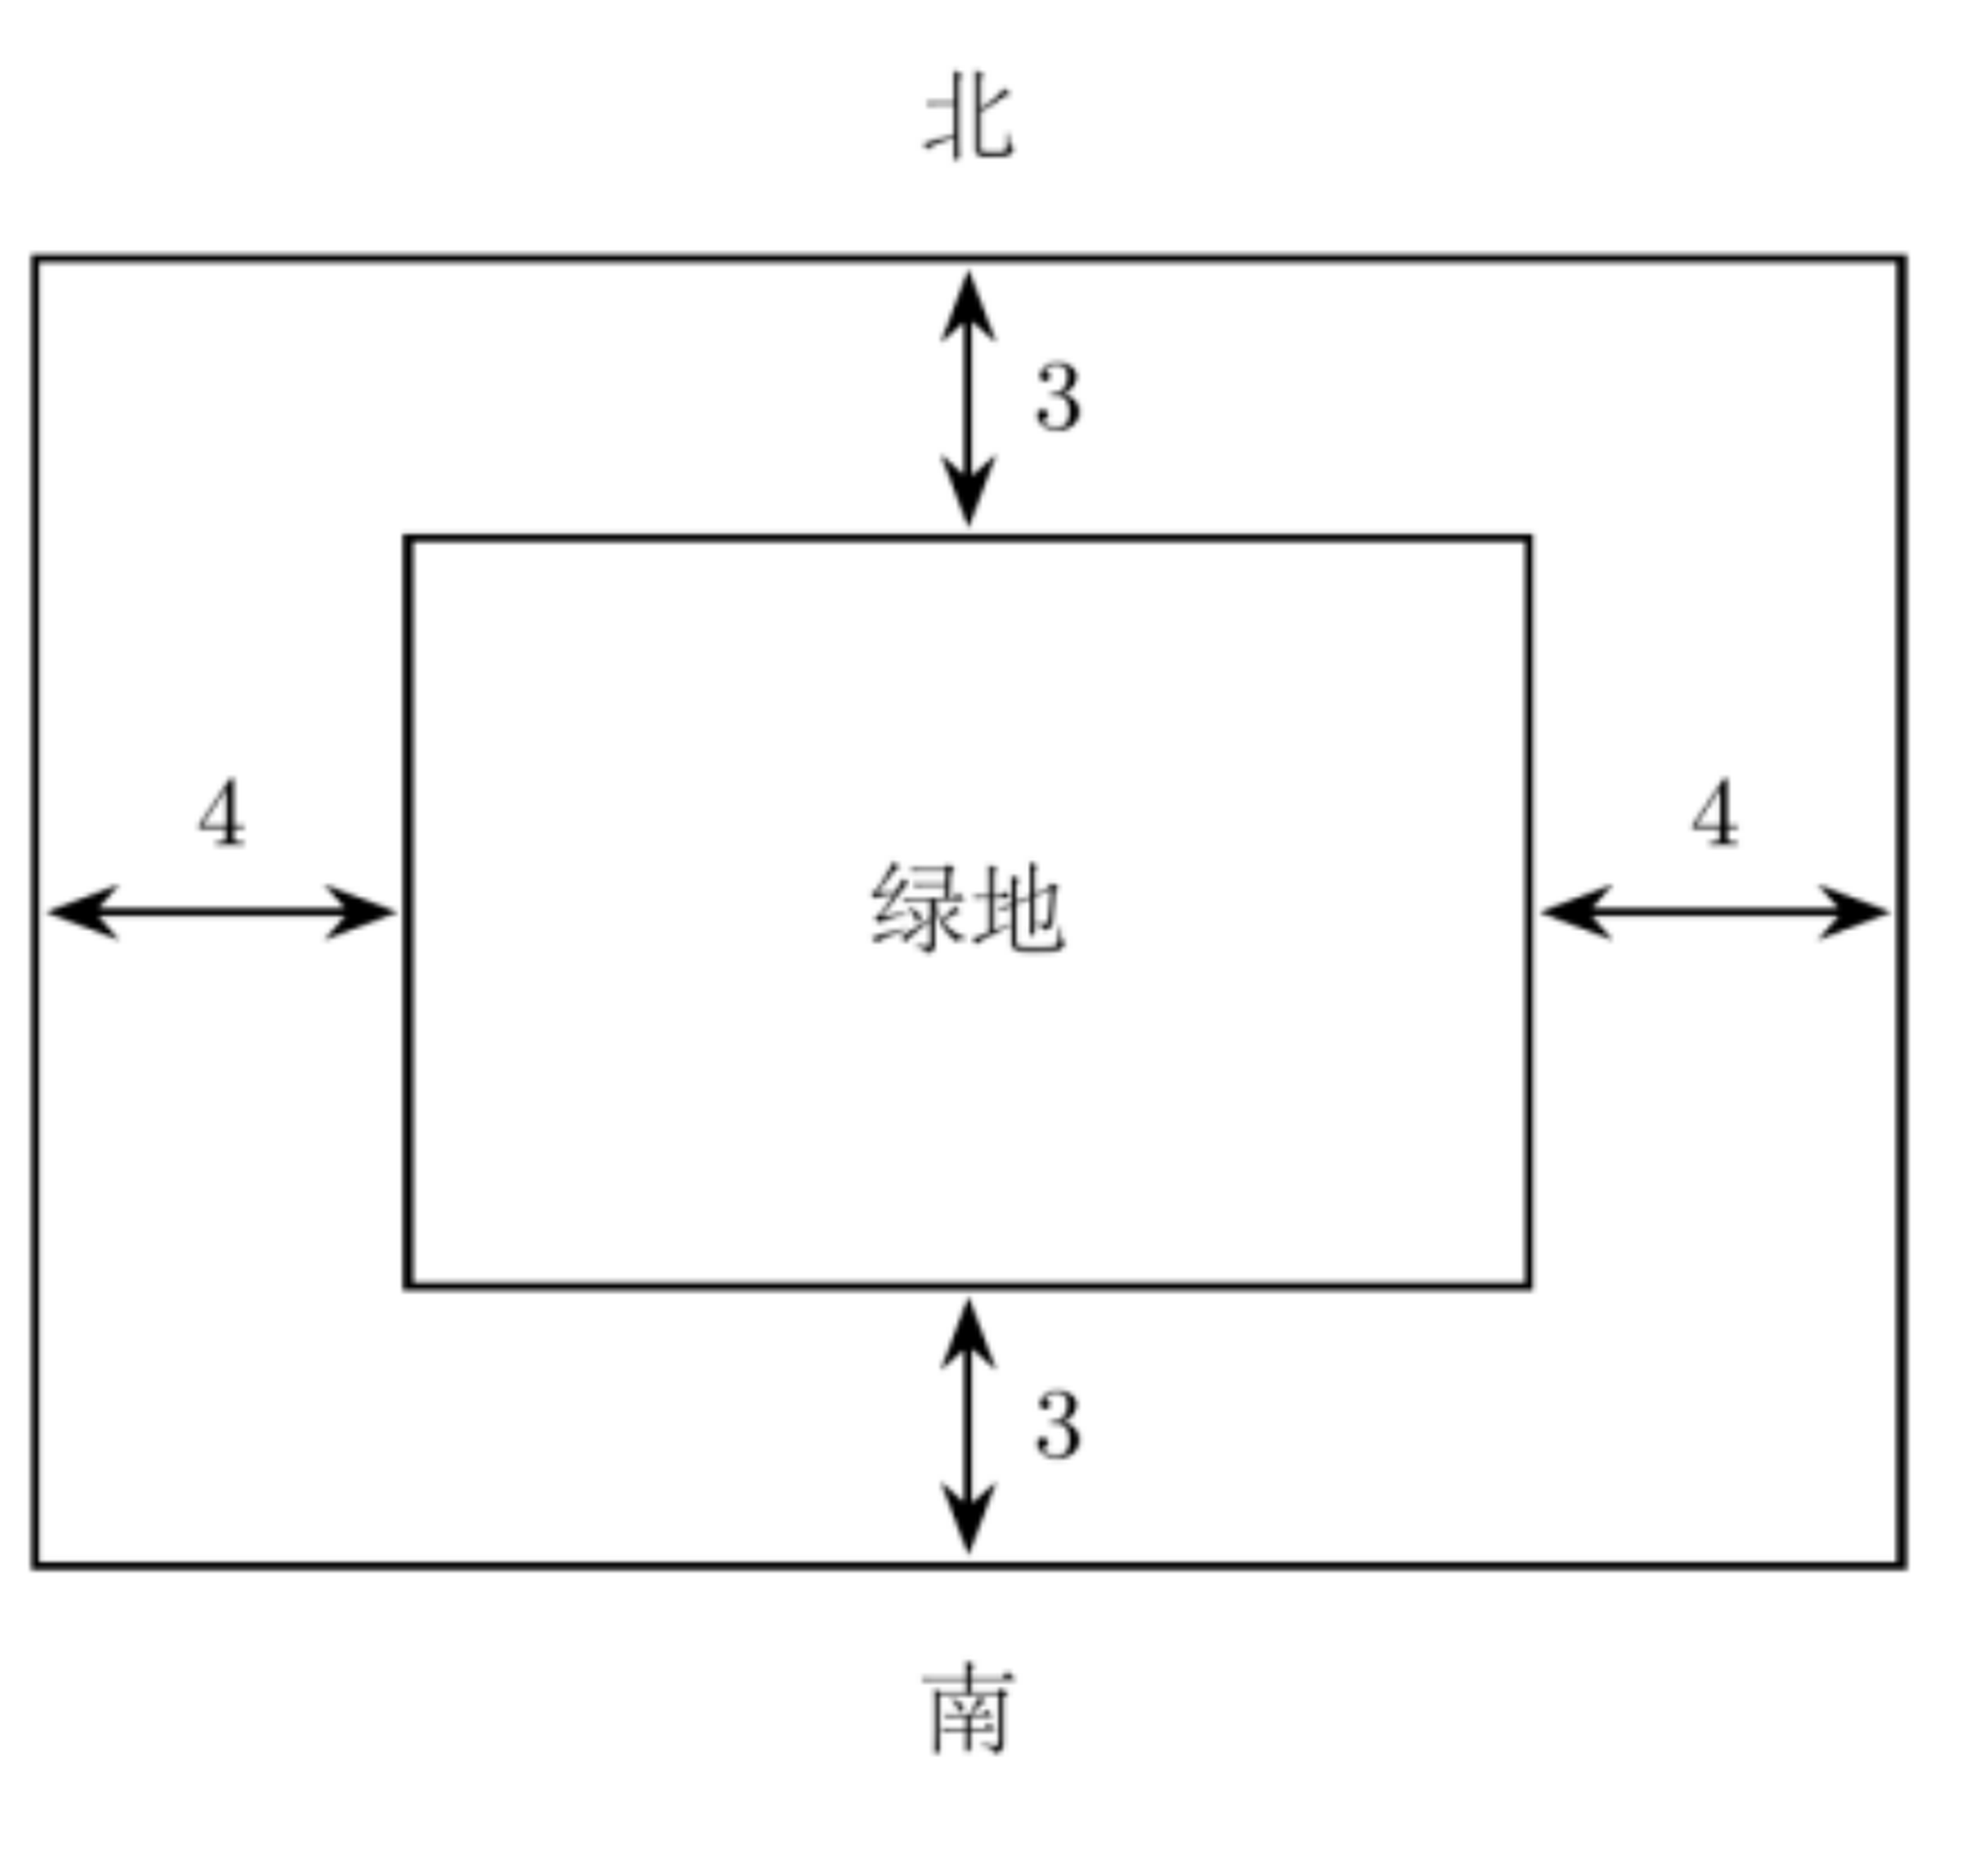
\includegraphics[width=0.32\textwidth]{figures/gao129_q19.png}
\end{center}

(1) 将 $S$ 表示为 $x$ 的函数；

(2) 试确定绿地东西方向的边长和南北方向的边长，使人行道的占地面积最小，并求出人行道的占地最小面积（结果精确到 0.1 米）

\ifanswer
\solbegin
\step{(1) 绿地南北方向的边长为 $\dfrac{1000}{x}$ 米，$x>0$.}
\step{外矩形东西、南北方向的边长分别为 $x+8$ 米、$\dfrac{1000}{x}+6$ 米.}
\step{因此 $S=(x+8)\left(\dfrac{1000}{x}+6\right)-1000=6x+\dfrac{8000}{x}+48, x>0$.}
\step{(2) 因为 $x>0,S=6x+\dfrac{8000}{x}+48\geqslant2\sqrt{6x\cdot\dfrac{8000}{x}}+48=48+80\sqrt{30}$.}
\step{等号当且仅当 $6x=\dfrac{8000}{x}$，即 $x=\dfrac{20\sqrt{30}}{3}\approx36.5$ 时成立，}
\step{此时绿地南北方向的边长为 $\dfrac{1000}{x}=\dfrac{1000}{\dfrac{20\sqrt{30}}{3}}=5\sqrt{30}\approx27.4$（米），}
\step{所以绿地东西方向、南北方向的边长分别约为 36.5 米、27.4 米时，}
\step{人行道的占地面积最小，最小面积为 $S_{min}=48+80\sqrt{30}\approx486.2$ 平方米.}
\solend
\fi

\item 已知集合 $A=\{x\mid x^2-3x+2=0\},B=\{x\mid x^2-ax+a-1=0\}$，

$C=\{x\mid x^2+2(m+1)x+m^2-5=0\}$.

(1) 若 $A=B$，求实数 $a$ 的值；

(2) 若 $B=\{1\}$，求实数 $a$ 的值；

(3) 若 $A\cap C=C$，求实数 $m$ 的取值范围.

\ifanswer
\solbegin
\step{(1) $A=\{1,2\}$，且 $x^2-ax+a-1=(x-1)(x-a+1)$，所以 $B=\{1,a-1\}$，}
\step{因此 $A=B\Leftrightarrow a-1=2\Leftrightarrow a=3$.}
\step{(2) $B=\{1\}$ 表示原方程只有一个不同的实数根，}
\step{得 $a-1=1$，即 $a=2$.}
\step{当 $a=2$ 时，原方程为 $(x-1)^2=0$，符合题意.}
\step{(3) $A\cap C=C\Leftrightarrow C\subseteq\{1,2\}$，}
\step{方程的判别式为 $\Delta=[2(m+1)]^2-4(m^2-5)=8(m+3)$.}
\step{当 $m<-3$ 时，$\Delta<0, C=\varnothing$，满足条件.}
\step{当 $m=-3$ 时，原方程为 $(x-2)^2=0, C=\{2\}$，满足条件.}
\step{当 $m>-3$ 时，方程有两个不同的实数根，必须有 $C=\{1,2\}$，}
\step{由韦达定理，$\begin{cases}-2(m+1)=1+2=3\\m^2-5=1\cdot2=2\end{cases}$，}
\step{第一式得 $m=-\dfrac52$，但此时 $m^2-5=\dfrac54\neq2$，不合题意.}
\step{因此 $m$ 的取值范围为 $(-\infty,-3]$.}
\solend
\fi

\item 设函数 $f(x)=ax^2+(1-a)x+a-2(a\in\R)$.

(1) 若关于 $x$ 的不等式 $f(x)\leqslant0$ 的解集为 $\left[0,\dfrac12\right]$，求实数 $a$ 的值；

(2) 若不等式 $f(x)\geqslant-2$ 对于实数 $a\in[-1,1]$ 时恒成立，求 $x$ 的取值范围；

(3) 解关于 $x$ 的不等式：$f(x)<a-1$.

\ifanswer
\solbegin
\step{(1) 由题意得 $0,\dfrac12$ 是方程 $ax^2+(1-a)x+a-2=0$ 的两个根，}
\step{则 $\begin{cases}0+\dfrac12=-\dfrac{1-a}{a}\\0\times\dfrac12=\dfrac{a-2}{a}\end{cases}\Rightarrow a=2$；}
\step{(2) $ax^2+(1-a)x+a-2\geqslant-2\Rightarrow a(x^2-x+1)+x\geqslant0$ 对 $a\in[-1,1]$ 恒成立，}
\step{则 $\begin{cases}-(x^2-x+1)+x\geqslant0\\(x^2-x+1)+x\geqslant0\end{cases}\Rightarrow\begin{cases}x=1\\x\in\R\end{cases}\Rightarrow x=1$，则 $x$ 的取值范围为 $\{1\}$；}
\step{(3) $f(x)<a-1$ 等价于 $ax^2+(1-a)x-1<0$，}
\step{当 $a=0$ 时，不等式可化为 $x<1$，解集为 $\{x\mid x<1\}$，}
\step{当 $a>0$ 时，不等式可化为 $(ax+1)(x-1)<0$，解集为 $\{x\mid -\dfrac1a<x<1\}$；}
\step{当 $a<0$ 时，不等式化为 $(ax+1)(x-1)<0$，}
\step{①当 $a=-1$ 时，$-\dfrac1a=1$，不等式的解集为 $\{x\mid x\neq1\}$；}
\step{②当 $-1<a<0$ 时，$-\dfrac1a>1$，不等式的解集为 $\{x\mid x<1$ 或 $x>-\dfrac1a\}$；}
\step{③当 $a<-1$ 时，$-\dfrac1a<1$，不等式的解集为 $\{x\mid x<-\dfrac1a$ 或 $x>1\}$；}
\step{综上，当 $a<-1$ 时，解集为 $\{x\mid x<-\dfrac1a$ 或 $x>1\}$；}
\step{当 $a=-1$ 时，解集为 $\{x\mid x\neq1\}$；}
\step{当 $-1<a<0$ 时，解集为 $\{x\mid x<1$ 或 $x>-\dfrac1a\}$；}
\step{当 $a=0$ 时，解集为 $\{x\mid x<1\}$；}
\step{当 $a>0$ 时，解集为 $\{x\mid -\dfrac1a<x<1\}$.}
\solend
\fi

\end{enumerate}

\end{document}
"
% 紧凑版：xelatex "\def\iscompact{1}% 高一129_立达中学_期中.tex
%   —— 高一上数学"2026-2027 年立达中学高一上期中"（试卷版/答案版）
% 试卷版：xelatex 高一129_立达中学_期中.tex
% 答案版：xelatex "\def\isanswer{1}\input{高一129_立达中学_期中.tex}"
% 紧凑版：xelatex "\def\iscompact{1}\input{高一129_立达中学_期中.tex}"
%
% 原始材料：微信公众号"魔都数学加油站"文章，作者破晓，2026-11-12 18:56 发布；
% 连载"27学年高一129"，原文标题"27学年高一129——2026-2027年上海市立达中学高一上期中"；
% 原文链接：https://mp.weixin.qq.com/s/gJhGsOBiWi7gW62u8EWLYA。
% 正文为 8 张 PNG 页（01、02、03、05、06 为 4762x6735，04、07、08 为 2560x3620），
% 题目下印有【解析】或【答案】，为讲评版。题目、解析均据原图转录；
% 卷面粉红色水印"魔都数学加油站"及公众号页脚未录入。全卷仅第 19 题有 1 幅插图。
%
% 卷首标题：原卷印作"2026-2027 年立达中学高一上期中"（公众号标题中的"上海市"
% 卷面标题行没有，本稿照卷面），年份区间按全稿惯例排 en dash；原卷未印副标题，
% 本卷为期中卷、跨集合与常用逻辑用语／不等式／函数三章，按题目内容标为
% "集合与常用逻辑用语、不等式、函数"（与 125、126 同为期中卷，口径相同）：
% 集合与逻辑见 Q3、Q4、Q13、Q20，不等式见 Q5、Q6、Q7、Q9、Q10、Q11、Q12、
% Q14、Q15、Q16、Q17、Q18、Q21，函数（含二次函数、基本不等式应用）见 Q8、Q19、Q21。
%
% 与原卷的排版差异：
%   ① 原文从第 3 题起，填空题编号为 3—12、选择题为 13—16、解答题为 17—21，本稿保留原题号；
%   ② 原卷每题下直接印【解析】／【答案】，本稿按全稿惯例置于答案版；第 3、5 题只印
%      【答案】，另提 \ans{}；第 13—16 题答案均在【解析】末句"故选 …"，题干括号内留空、
%      不另提 \ans{}；四道选择题括号内原卷均未印答案；
%   ③ 原卷未印副标题，本稿按"知识模块"口径补出（见上"卷首标题"）；
%   ④ 原卷填空横线按全稿惯例排为 \blankline[4.4em]；选择题括号排 \mbox{（\quad）}、
%      选项段前按惯例加 \keepwithprev；解答题不留作答区（原卷为讲评版，与 109—128 同）；
%   ⑤ 原卷数集排斜体 $R$，按全稿惯例改 \R；绝对值排 \lvert…\rvert，集合描述竖线排 \mid；
%      不等号按全稿惯例排 \leqslant／\geqslant；子题标号原卷一律用半角括号 (1)(2)(3)，本稿照录；
%   ⑥ 原卷第 19 题插图浮排在 Q18 解析右侧、"19."题干之上，本稿按体例就近置于 Q19
%      题干"如图所示"之后（居中 \includegraphics），图取原卷截图去水印；题前按惯例加
%      \needvspace{7cm} 守卫（照 高一120／127 成例），保证"题干 + 图"整块不被页边界切开；
%   ⑦ 原卷 Q8 解析续头印在第 2 页页首、Q17 解析续头印在第 5 页页首、Q19 题干续在第 6 页、
%      Q20 解析跨 6—7 页、Q21 解析续头印在第 8 页页首，本稿按题合并连续排版；
%      末页第 8 页为 Q21 解析的续尾，按实际印刷行单列（照 高一127 第 09 页续尾成例）。
%
% 判别式字形：第 8 题解析 $\Delta=m^2+4m>0$、第 10 题解析 $\Delta=k^2+6k=k(k+6)<0$、
%   第 20 题 (3) 解析 $\Delta=[2(m+1)]^2-4(m^2-5)=8(m+3)$ 三处原卷均排 $\Delta$
%   （等腰、高；回原图逐处放大核对、三处字形一致），照录 \Delta；全卷未出现 \triangle
%   （等边、扁）。
%
% 子集符号：第 13 题 ② $\{0,1,2\}\subseteq\{2,1,0\}$、③ $\varnothing\subseteq\{0,1,2\}$，
%   第 17 题 (2)② $B\subseteq A$、$B\subseteq(3,+\infty)$，第 20 题 (3) $C\subseteq\{1,2\}$
%   均印带下划线，照录 \subseteq；全卷未出现单线 \subset（回原图放大逐处确认）。
%
% 原卷存疑照录：
%   第 15 题解析"即 $m=4$，$n=3$ 时取等号"与题干 $\dfrac1m+n=1$、等号条件
%     $mn=\dfrac9{mn}$ 均不一致（按题应为 $n=\dfrac34$），照录、未统一；
%   第 18 题 (1) 题干"设 $M=2x^2+3x-1,N=7x-3$ 比较 $M$ 与 $N$ 两个数的大小"
%     两式间用半角逗号、且"$N=7x-3$"后无标点直接接"比较"，照录；
%   第 11 题解析"$1-x+2x-1=-(3x-2), 4x=2, x=\dfrac12$"、第 14 题解析
%     "$a=2, b=1, c=4, d=0$"、第 19 题解析"$6x+\dfrac{8000}{x}+48, x>0$"、
%     第 20 题解析"$\Delta<0, C=\varnothing$"与"$(x-2)^2=0, C=\{2\}$"、
%     第 12 题解析"$(x+y)^2=3+t\geqslant0,(x-y)^2=3-3t\geqslant0$"等处数学式内
%     用半角逗号，照录；
%   第 19 题题干"如图所示（图中单位：米）设绿地东西方向的边长为 $x$"在右括号后
%     无标点直接续"设"，照录；
%   第 21 题 (3) 解析先按 $a>0$、$a=0$、$a<0$ 分述解集，又在"综上"处重列全部
%     五类（含已给出的 $a>0$、$a=0$），照录；
%   第 21 题 (2) 题干与解析均作 $f(x)\geqslant-2$（与 $a(x^2-x+1)+x\geqslant0$ 相符），
%     照录，勿误读为 $f(x)\geqslant2$。
%
% 行数复核：逐题数 \step 条数，合计 93 条（Q3：0；Q4：2；Q5：0；Q6：3；Q7：3；
% Q8：2；Q9：4；Q10：3；Q11：5；Q12：5；Q13：1；Q14：3；Q15：3；Q16：7；
% Q17：7；Q18：8；Q19：8；Q20：13；Q21：16），与原卷印刷行逐题相等
% （cases 块作一个印刷行计）。第 3、5 题只印【答案】，提 \ans{}，不计入 \step 账；
% 四道选择题答案均在解析末句，括号内留空、不另提 \ans{}。
%
\documentclass[a4paper,11pt]{article}
\usepackage{common}

\begin{document}

\examtitlest[3]{2026--2027 年立达中学高一上期中}{集合与常用逻辑用语、不等式、函数}

\bigsec{一、填空题}

\begin{enumerate}
\setcounter{enumi}{2}

\item 若 $A=\{x\mid -3<x\leqslant2\},B=\{x\mid 1<x\leqslant3\}$，则 $A\cup B=$\blankline[4.4em].

\ifanswer
\ans{$(-3,3]$}
\fi

\item 若 $A$ 是 $B$ 的必要非充分条件，$B$ 是 $C$ 的充要条件，$C$ 是 $D$ 的必要非充分条件，则 $D$ 是 $A$ 的\blankline[4.4em]条件.

\ifanswer
\solbegin
\step{$D\Rightarrow C\Leftrightarrow B\Rightarrow A$，且 $A\nRightarrow B$，因此 $D\Rightarrow A$ 且 $A\nRightarrow D$，}
\step{故 $D$ 是 $A$ 的充分非必要条件.}
\solend
\fi

\item 不等式 $\dfrac1x<1$ 的解集为\blankline[4.4em].

\ifanswer
\ans{$(-\infty,0)\cup(1,+\infty)$}
\fi

\item 已知正实数 $x$、$y$ 满足 $2x+y=2$，则 $xy$ 的最大值为\blankline[4.4em].

\ifanswer
\solbegin
\step{因为 $x>0$，$y>0$，所以 $2x+y\geqslant2\sqrt{2xy}$（当且仅当 $2x=y$ 时，取等号），}
\step{又因为 $2x+y=2$，所以 $2\geqslant2\sqrt{2xy}$（当且仅当 $2x=y$ 时，取等号），}
\step{即 $xy\leqslant\dfrac12$，则 $xy$ 的最大值为 $\dfrac12$.}
\solend
\fi

\item 已知 $x\in\R$，函数 $y=\lvert x+2\rvert+\lvert x-3\rvert$ 的最小值为\blankline[4.4em].

\ifanswer
\solbegin
\step{由 $\lvert x+2\rvert+\lvert x-3\rvert\geqslant\lvert(x+2)-(x-3)\rvert=5$，}
\step{当且仅当 $(x+2)(x-3)\leqslant0$，即 $-2\leqslant x\leqslant3$ 时，上式取等号，}
\step{则函数 $y=\lvert x+2\rvert+\lvert x-3\rvert$ 的最小值是 5.}
\solend
\fi

\item 已知实系数一元二次方程 $x^2+mx-m=0$ 的两根分别为 $x_1,x_2$，且 $\lvert x_1-x_2\rvert=\sqrt{21}$，实数 $m$ 的值为\blankline[4.4em].

\ifanswer
\solbegin
\step{由题意得 $\Delta=m^2+4m>0$，解得 $m>0$ 或 $m<-4,x_1+x_2=-m,x_1x_2=-m$，}
\step{则 $\lvert x_1-x_2\rvert=\sqrt{(x_1+x_2)^2-4x_1x_2}=\sqrt{m^2+4m}=\sqrt{21}$，解得 $m=-7$ 或 $3$.}
\solend
\fi

\item 已知不等式 $ax^2-5x+b>0$ 的解集是 $\{x\mid -3<x<-2\}$，则不等式 $bx^2-5x+a>0$ 的解集是\blankline[4.4em].

\ifanswer
\solbegin
\step{$ax^2-5x+b=a(x+3)(x+2)$，比较系数得 $5a=-5,b=6a$，}
\step{即 $a=-1,b=-6$.}
\step{$bx^2-5x+a>0\Leftrightarrow(3x+1)(2x+1)<0\Leftrightarrow-\dfrac12<x<-\dfrac13$，}
\step{故解集为 $\left\{x\mid -\dfrac12<x<-\dfrac13\right\}$.}
\solend
\fi

\item 不等式 $4kx^2+kx-\dfrac38<0$ 对于一切实数 $x$ 都成立，则实数 $k$ 的取值范围是\blankline[4.4em].

\ifanswer
\solbegin
\step{$k=0$ 时，不等式恒成立；}
\step{$k\neq0$ 时，须 $4k<0$ 且 $\Delta=k^2+6k=k(k+6)<0$，解得 $-6<k<0$.}
\step{因此 $k\in(-6,0]$.}
\solend
\fi

\item 设 $x\in\R$，方程 $\lvert 1-x\rvert+\lvert 2x-1\rvert=\lvert 3x-2\rvert$ 的解集为\blankline[4.4em].

\ifanswer
\solbegin
\step{当 $x\leqslant\dfrac12$ 时，方程化为 $1-x-(2x-1)=-(3x-2)$，$2-3x=-3x+2$，恒成立，}
\step{当 $\dfrac12<x\leqslant\dfrac23$ 时，方程化为 $1-x+2x-1=-(3x-2), 4x=2, x=\dfrac12$，不合题意，}
\step{当 $\dfrac23<x\leqslant1$ 时，方程化为 $1-x+2x-1=3x-2$，$2x=2$，解得 $x=1$，}
\step{当 $x>1$ 时，方程化为 $-(1-x)+2x-1=3x-2$，$3x-2=3x-2$，恒成立，}
\step{综上所述，$\lvert 1-x\rvert+\lvert 2x-1\rvert=\lvert 3x-2\rvert$ 的解集为 $\left(-\infty,\dfrac12\right]\cup[1,+\infty)$.}
\solend
\fi

\item 已知非零实数 $x,y$ 满足 $x^2+xy+y^2=3$，则 $x^2-xy+y^2$ 的取值范围是\blankline[4.4em].

\ifanswer
\solbegin
\step{令 $t=xy\neq0$，由 $(x+y)^2=3+t\geqslant0,(x-y)^2=3-3t\geqslant0$，}
\step{得 $t\in[-3,0)\cup(0,1]$.}
\step{对上述任意 $t$，联立 $x+y=\sqrt{3+t},x-y=\sqrt{3-3t}$，所得 $x,y$ 满足原条件，}
\step{因此上述 $t$ 均可取到.}
\step{于是 $x^2-xy+y^2=3-2t$ 的取值范围为 $[1,3)\cup(3,9]$.}
\solend
\fi

\end{enumerate}

\bigsec{二、选择题}

\begin{enumerate}
\setcounter{enumi}{12}

\item 下列各式中，正确的个数是\mbox{（\quad）}

① $\{0\}\in\{0,1,2\}$；② $\{0,1,2\}\subseteq\{2,1,0\}$；③ $\varnothing\subseteq\{0,1,2\}$；④ $\varnothing=\{0\}$；⑤ $\{0,1\}=\{(0,1)\}$；

⑥ $0=\{0\}$.

\keepwithprev
A. $1$\qquad\qquad B. $2$\qquad\qquad C. $3$\qquad\qquad D. $4$

\ifanswer
\solbegin
\step{①不正确，②正确，③正确，④不正确，⑤不正确，⑥不正确. 故选 $B$.}
\solend
\fi

\item 下列四个命题中，为真命题的是\mbox{（\quad）}

\keepwithprev
A. 若 $a>b$，则 $ac^2>bc^2$\qquad\qquad B. 若 $a>b,c>d$，则 $a-c>b-d$

C. 若 $ac^2>bc^2$，则 $a>b$\qquad\qquad D. 若 $a>b$，则 $\dfrac1a<\dfrac1b$

\ifanswer
\solbegin
\step{C 中，$(a-b)c^2>0$，必有 $c^2>0$ 且 $a-b>0$，即 $a>b$.}
\step{A 取 $c=0$；B 取 $a=2, b=1, c=4, d=0$；D 取 $a=1, b=-1$，均不成立.}
\step{故选 $C$.}
\solend
\fi

\item 已知 $m$、$n\in(0,+\infty)$，$\dfrac1m+n=1$，则 $m+\dfrac9n$ 的最小值为\mbox{（\quad）}

\keepwithprev
A. $13$\qquad\qquad B. $16$\qquad\qquad C. $3$\qquad\qquad D. $6$

\ifanswer
\solbegin
\step{因为 $m$、$n\in(0,+\infty)$，$\dfrac1m+n=1$，}
\step{所以 $m+\dfrac9n=(m+\dfrac9n)(\dfrac1m+n)=10+mn+\dfrac9{mn}\geqslant10+2\sqrt{mn\cdot\dfrac9{mn}}=16$，}
\step{当且仅当 $mn=\dfrac9{mn}$，即 $m=4$，$n=3$ 时取等号. 故选 $B$.}
\solend
\fi

\item 下列不等式：① $\left\lvert x+\dfrac1x\right\rvert\geqslant2$；② $x^2+2x+1>0$；③ $\lvert x\rvert+\lvert x-1\rvert\geqslant1$；④ $\dfrac{x}{x^2+x+1}<1$；

解集为 $\R$ 的不等式的个数是\mbox{（\quad）}

\keepwithprev
A. $0$\qquad\qquad B. $1$\qquad\qquad C. $2$\qquad\qquad D. $3$

\ifanswer
\solbegin
\step{对于①，当 $x=0$ 时，$\dfrac1x$ 无意义，故 $\left\lvert x+\dfrac1x\right\rvert\geqslant2$ 的解集不是 $\R$，错误；}
\step{对于②，$x^2+2x+1=(x+1)^2\geqslant0$，当 $x=-1$ 取到等号，解集不是 $\R$，故错误；}
\step{对于③，$\lvert x\rvert+\lvert x-1\rvert\geqslant\lvert x-(x-1)\rvert=1$，当 $x(x-1)\leqslant0$ 时取等号，解集为 $\R$，}
\step{故正确；}
\step{对于④，由于 $x^2+x+1>0$ 恒成立，}
\step{故 $\dfrac{x}{x^2+x+1}<1$ 等价于 $x<x^2+x+1\Rightarrow x^2+1>0$ 恒成立，故解集为 $\R$，正确，}
\step{故正确的有③④，故选 $C$.}
\solend
\fi

\end{enumerate}

\bigsec{三、解答题}

\begin{enumerate}
\setcounter{enumi}{16}

\item (1) 解不等式组 $\begin{cases}\dfrac{x+3}{x+1}\leqslant2\\\lvert 2x-3\rvert\leqslant2\end{cases}$.

(2) 已知集合 $A=\{x\mid -x+3<0\},B=\{x\mid a\leqslant x\leqslant a+3\}$.

①当 $a=2$，求集合 $A\cap B$；

②若 $A\cup B=A$，求实数 $a$ 的取值范围.

\ifanswer
\solbegin
\step{(1) 由 $\begin{cases}\dfrac{x+3}{x+1}\leqslant2\\\lvert 2x-3\rvert\leqslant2\end{cases}$ 得 $\begin{cases}\dfrac{x+3-2x-2}{x+1}\leqslant0\\-2\leqslant2x-3\leqslant2\end{cases}$，即 $\begin{cases}\dfrac{-x+1}{x+1}\leqslant0\\1\leqslant2x\leqslant5\end{cases}$，则 $\begin{cases}\dfrac{x-1}{x+1}\geqslant0\\\dfrac12\leqslant x\leqslant\dfrac52\end{cases}$，}
\step{解得 $1\leqslant x\leqslant\dfrac52$，即原不等式组的解集为 $\left[1,\dfrac52\right]$.}
\step{(2) $-x+3<0\Leftrightarrow x>3$，所以 $A=(3,+\infty)$.}
\step{①当 $a=2$ 时，$B=[2,5], A\cap B=(3,+\infty)\cap[2,5]=(3,5]$.}
\step{②$A\cup B=A\Leftrightarrow B\subseteq A$.}
\step{因为 $B=[a,a+3]$，且左端点 $a\in B$，所以 $B\subseteq(3,+\infty)\Leftrightarrow a>3$，}
\step{实数 $a$ 的取值范围为 $(3,+\infty)$.}
\solend
\fi

\item (1) 设 $M=2x^2+3x-1,N=7x-3$ 比较 $M$ 与 $N$ 两个数的大小.

(2) 解关于 $x$ 的不等式：$x^2-(a+3)x+3a<0$，$a\in\R$.

\ifanswer
\solbegin
\step{(1) $M-N=2x^2+3x-1-(7x-3)=2(x-1)^2$.}
\step{$x=1$ 时，$M-N=0$，即 $M=N$.}
\step{$x\neq1$ 时，$M-N>0$，即 $M>N$.}
\step{(2) 不等式 $x^2-(a+3)x+3a<0$ 可化为 $(x-3)(x-a)<0$，}
\step{不等式对应方程的解为 $a$ 和 3，}
\step{当 $a<3$ 时，不等式 $x^2-(a+3)x+3a<0$ 的解集为 $(a,3)$，}
\step{当 $a=3$ 时，不等式 $x^2-(a+3)x+3a<0$ 的解集为 $\varnothing$，}
\step{当 $a>3$ 时，不等式 $x^2-(a+3)x+3a<0$ 的解集为 $(3,a)$.}
\solend
\fi

% 第 19 题是"题干 + 图"约 7cm 的一整块，答案版实测断点落在题干之后（图被推到次页页首），
% 照 高一120／127 成例在题前先量一次页高，不够就把"题干 + 图"整块一起挪到次页。
\needvspace{7cm}
\item 某新建居民小区欲建一面积为 1000 平方米的矩形绿地，在绿地四周铺设人行道，设计要求绿地南北两侧人行道宽 3 米，东西两侧人行道宽 4 米，如图所示（图中单位：米）设绿地东西方向的边长为 $x$，人行道的占地面积为 $S$.

\begin{center}
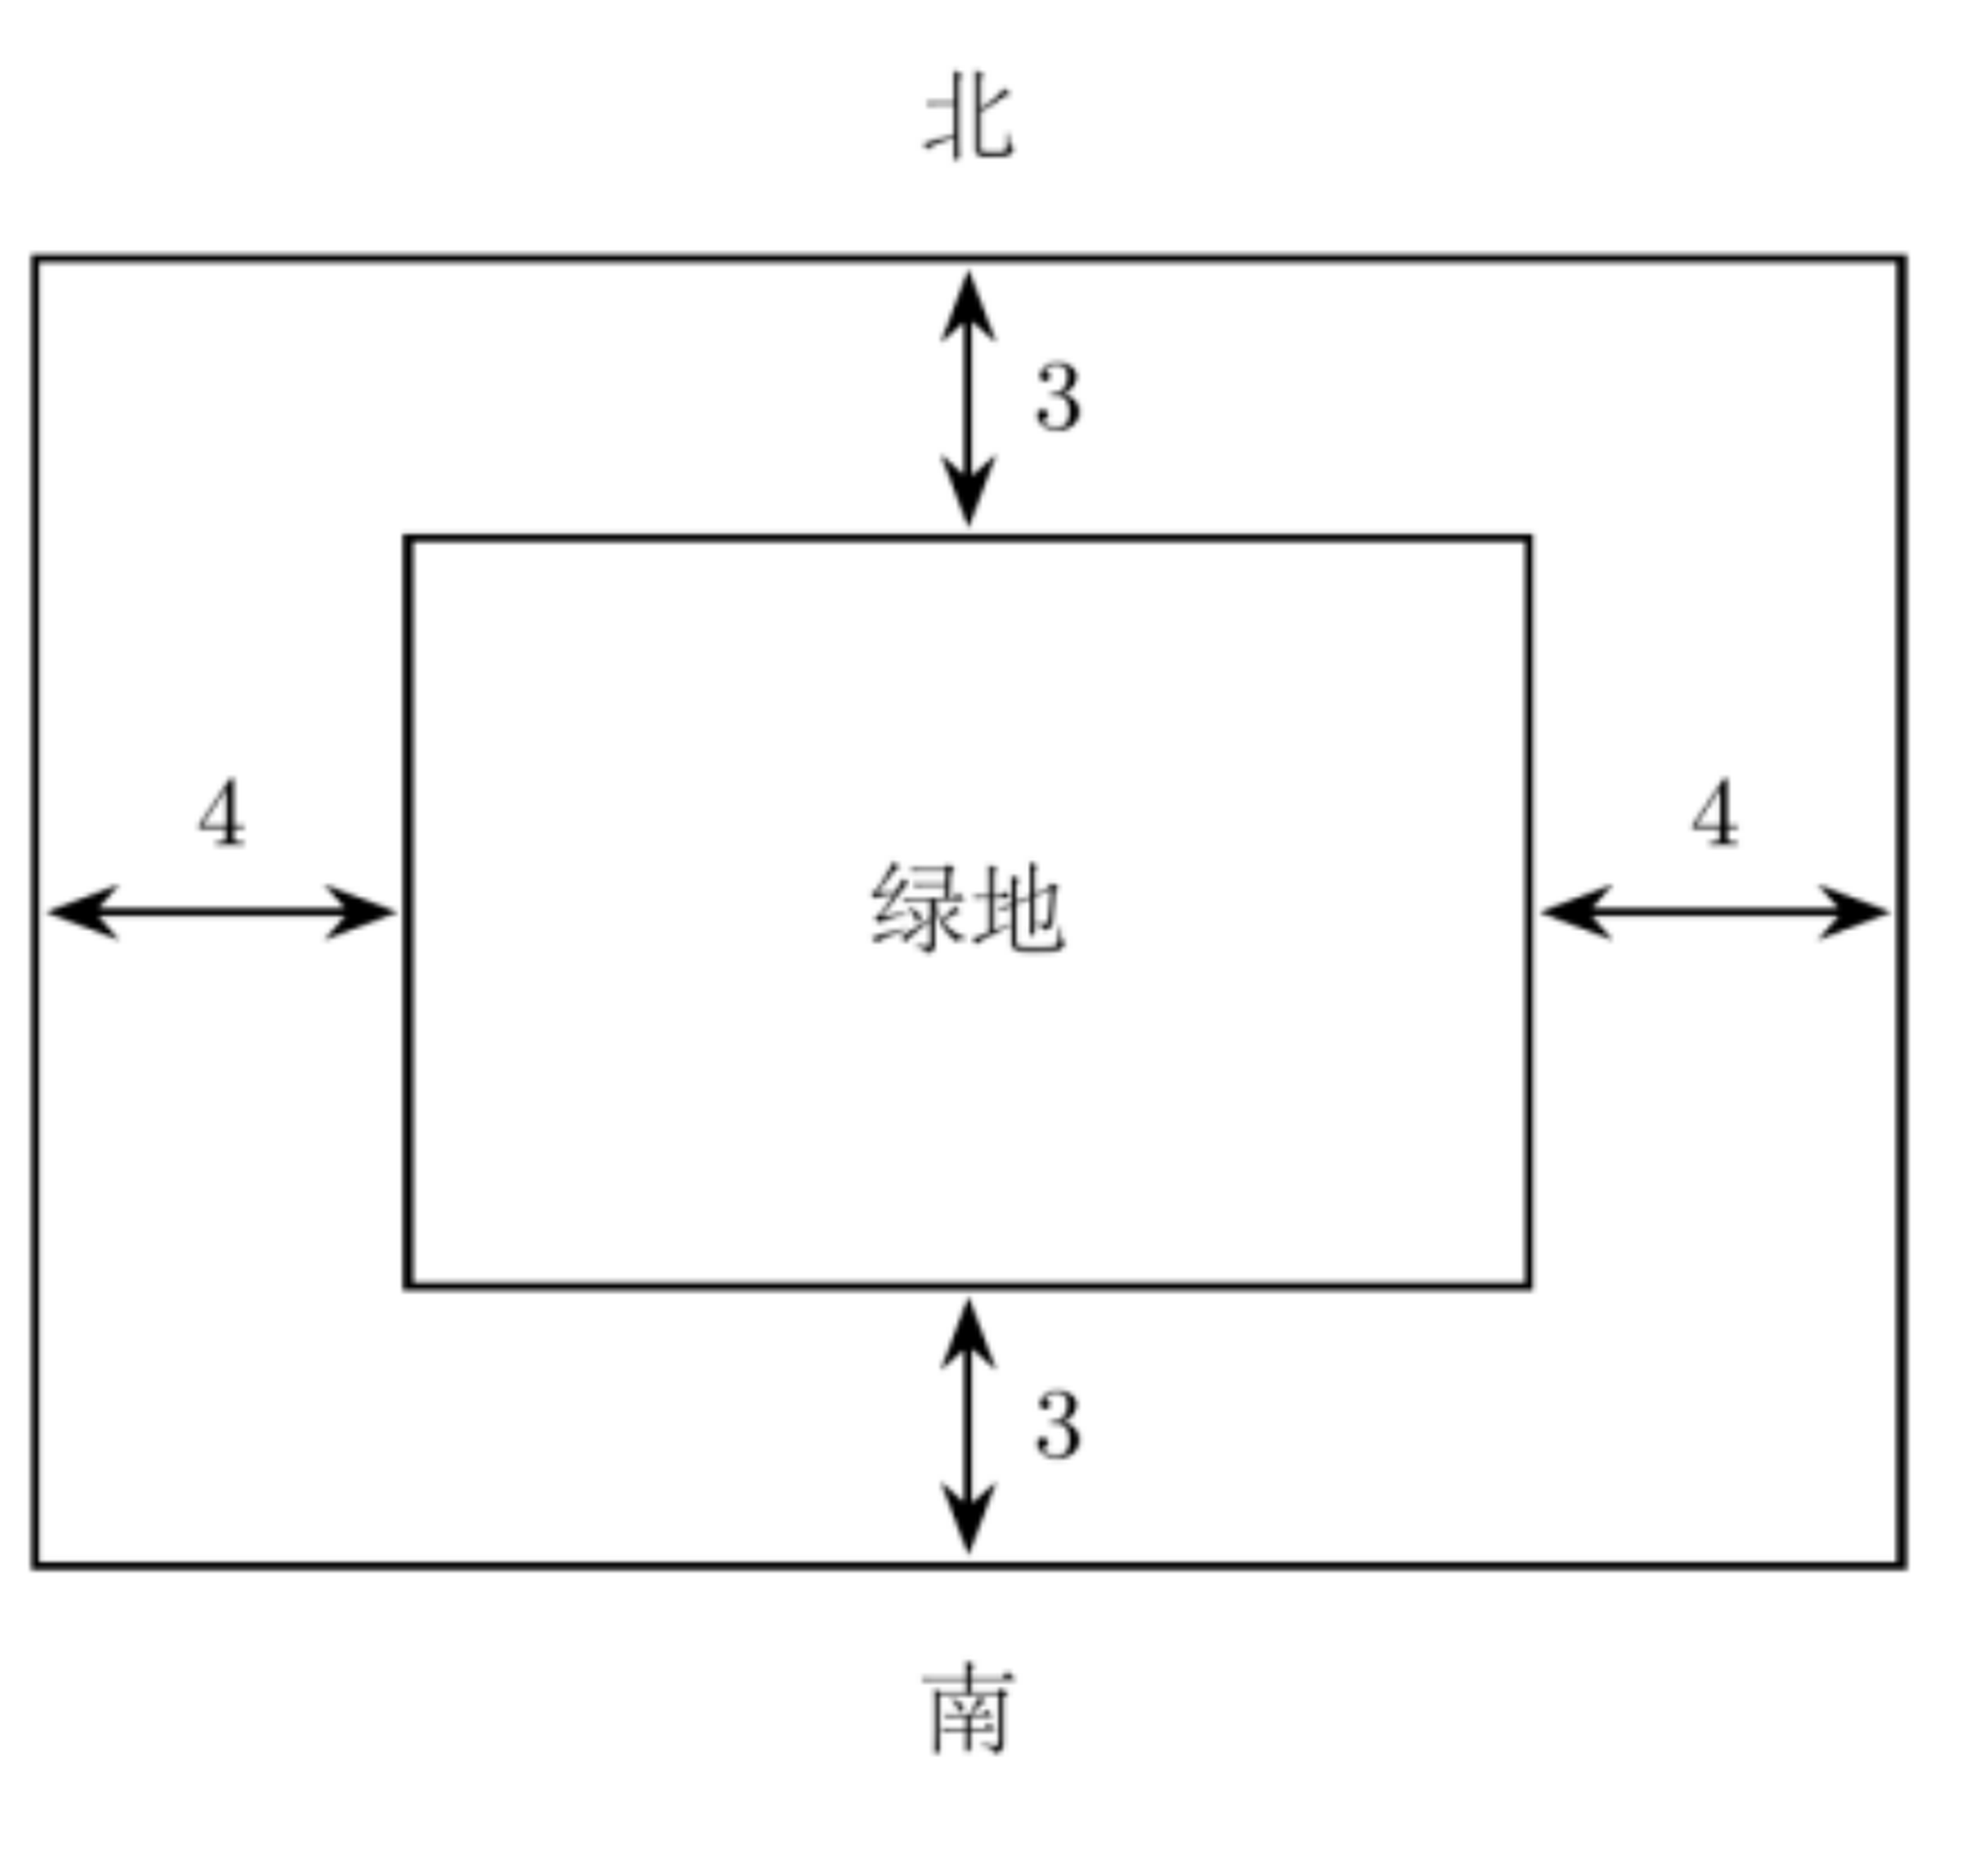
\includegraphics[width=0.32\textwidth]{figures/gao129_q19.png}
\end{center}

(1) 将 $S$ 表示为 $x$ 的函数；

(2) 试确定绿地东西方向的边长和南北方向的边长，使人行道的占地面积最小，并求出人行道的占地最小面积（结果精确到 0.1 米）

\ifanswer
\solbegin
\step{(1) 绿地南北方向的边长为 $\dfrac{1000}{x}$ 米，$x>0$.}
\step{外矩形东西、南北方向的边长分别为 $x+8$ 米、$\dfrac{1000}{x}+6$ 米.}
\step{因此 $S=(x+8)\left(\dfrac{1000}{x}+6\right)-1000=6x+\dfrac{8000}{x}+48, x>0$.}
\step{(2) 因为 $x>0,S=6x+\dfrac{8000}{x}+48\geqslant2\sqrt{6x\cdot\dfrac{8000}{x}}+48=48+80\sqrt{30}$.}
\step{等号当且仅当 $6x=\dfrac{8000}{x}$，即 $x=\dfrac{20\sqrt{30}}{3}\approx36.5$ 时成立，}
\step{此时绿地南北方向的边长为 $\dfrac{1000}{x}=\dfrac{1000}{\dfrac{20\sqrt{30}}{3}}=5\sqrt{30}\approx27.4$（米），}
\step{所以绿地东西方向、南北方向的边长分别约为 36.5 米、27.4 米时，}
\step{人行道的占地面积最小，最小面积为 $S_{min}=48+80\sqrt{30}\approx486.2$ 平方米.}
\solend
\fi

\item 已知集合 $A=\{x\mid x^2-3x+2=0\},B=\{x\mid x^2-ax+a-1=0\}$，

$C=\{x\mid x^2+2(m+1)x+m^2-5=0\}$.

(1) 若 $A=B$，求实数 $a$ 的值；

(2) 若 $B=\{1\}$，求实数 $a$ 的值；

(3) 若 $A\cap C=C$，求实数 $m$ 的取值范围.

\ifanswer
\solbegin
\step{(1) $A=\{1,2\}$，且 $x^2-ax+a-1=(x-1)(x-a+1)$，所以 $B=\{1,a-1\}$，}
\step{因此 $A=B\Leftrightarrow a-1=2\Leftrightarrow a=3$.}
\step{(2) $B=\{1\}$ 表示原方程只有一个不同的实数根，}
\step{得 $a-1=1$，即 $a=2$.}
\step{当 $a=2$ 时，原方程为 $(x-1)^2=0$，符合题意.}
\step{(3) $A\cap C=C\Leftrightarrow C\subseteq\{1,2\}$，}
\step{方程的判别式为 $\Delta=[2(m+1)]^2-4(m^2-5)=8(m+3)$.}
\step{当 $m<-3$ 时，$\Delta<0, C=\varnothing$，满足条件.}
\step{当 $m=-3$ 时，原方程为 $(x-2)^2=0, C=\{2\}$，满足条件.}
\step{当 $m>-3$ 时，方程有两个不同的实数根，必须有 $C=\{1,2\}$，}
\step{由韦达定理，$\begin{cases}-2(m+1)=1+2=3\\m^2-5=1\cdot2=2\end{cases}$，}
\step{第一式得 $m=-\dfrac52$，但此时 $m^2-5=\dfrac54\neq2$，不合题意.}
\step{因此 $m$ 的取值范围为 $(-\infty,-3]$.}
\solend
\fi

\item 设函数 $f(x)=ax^2+(1-a)x+a-2(a\in\R)$.

(1) 若关于 $x$ 的不等式 $f(x)\leqslant0$ 的解集为 $\left[0,\dfrac12\right]$，求实数 $a$ 的值；

(2) 若不等式 $f(x)\geqslant-2$ 对于实数 $a\in[-1,1]$ 时恒成立，求 $x$ 的取值范围；

(3) 解关于 $x$ 的不等式：$f(x)<a-1$.

\ifanswer
\solbegin
\step{(1) 由题意得 $0,\dfrac12$ 是方程 $ax^2+(1-a)x+a-2=0$ 的两个根，}
\step{则 $\begin{cases}0+\dfrac12=-\dfrac{1-a}{a}\\0\times\dfrac12=\dfrac{a-2}{a}\end{cases}\Rightarrow a=2$；}
\step{(2) $ax^2+(1-a)x+a-2\geqslant-2\Rightarrow a(x^2-x+1)+x\geqslant0$ 对 $a\in[-1,1]$ 恒成立，}
\step{则 $\begin{cases}-(x^2-x+1)+x\geqslant0\\(x^2-x+1)+x\geqslant0\end{cases}\Rightarrow\begin{cases}x=1\\x\in\R\end{cases}\Rightarrow x=1$，则 $x$ 的取值范围为 $\{1\}$；}
\step{(3) $f(x)<a-1$ 等价于 $ax^2+(1-a)x-1<0$，}
\step{当 $a=0$ 时，不等式可化为 $x<1$，解集为 $\{x\mid x<1\}$，}
\step{当 $a>0$ 时，不等式可化为 $(ax+1)(x-1)<0$，解集为 $\{x\mid -\dfrac1a<x<1\}$；}
\step{当 $a<0$ 时，不等式化为 $(ax+1)(x-1)<0$，}
\step{①当 $a=-1$ 时，$-\dfrac1a=1$，不等式的解集为 $\{x\mid x\neq1\}$；}
\step{②当 $-1<a<0$ 时，$-\dfrac1a>1$，不等式的解集为 $\{x\mid x<1$ 或 $x>-\dfrac1a\}$；}
\step{③当 $a<-1$ 时，$-\dfrac1a<1$，不等式的解集为 $\{x\mid x<-\dfrac1a$ 或 $x>1\}$；}
\step{综上，当 $a<-1$ 时，解集为 $\{x\mid x<-\dfrac1a$ 或 $x>1\}$；}
\step{当 $a=-1$ 时，解集为 $\{x\mid x\neq1\}$；}
\step{当 $-1<a<0$ 时，解集为 $\{x\mid x<1$ 或 $x>-\dfrac1a\}$；}
\step{当 $a=0$ 时，解集为 $\{x\mid x<1\}$；}
\step{当 $a>0$ 时，解集为 $\{x\mid -\dfrac1a<x<1\}$.}
\solend
\fi

\end{enumerate}

\end{document}
"
%
% 原始材料：微信公众号"魔都数学加油站"文章，作者破晓，2026-11-12 18:56 发布；
% 连载"27学年高一129"，原文标题"27学年高一129——2026-2027年上海市立达中学高一上期中"；
% 原文链接：https://mp.weixin.qq.com/s/gJhGsOBiWi7gW62u8EWLYA。
% 正文为 8 张 PNG 页（01、02、03、05、06 为 4762x6735，04、07、08 为 2560x3620），
% 题目下印有【解析】或【答案】，为讲评版。题目、解析均据原图转录；
% 卷面粉红色水印"魔都数学加油站"及公众号页脚未录入。全卷仅第 19 题有 1 幅插图。
%
% 卷首标题：原卷印作"2026-2027 年立达中学高一上期中"（公众号标题中的"上海市"
% 卷面标题行没有，本稿照卷面），年份区间按全稿惯例排 en dash；原卷未印副标题，
% 本卷为期中卷、跨集合与常用逻辑用语／不等式／函数三章，按题目内容标为
% "集合与常用逻辑用语、不等式、函数"（与 125、126 同为期中卷，口径相同）：
% 集合与逻辑见 Q3、Q4、Q13、Q20，不等式见 Q5、Q6、Q7、Q9、Q10、Q11、Q12、
% Q14、Q15、Q16、Q17、Q18、Q21，函数（含二次函数、基本不等式应用）见 Q8、Q19、Q21。
%
% 与原卷的排版差异：
%   ① 原文从第 3 题起，填空题编号为 3—12、选择题为 13—16、解答题为 17—21，本稿保留原题号；
%   ② 原卷每题下直接印【解析】／【答案】，本稿按全稿惯例置于答案版；第 3、5 题只印
%      【答案】，另提 \ans{}；第 13—16 题答案均在【解析】末句"故选 …"，题干括号内留空、
%      不另提 \ans{}；四道选择题括号内原卷均未印答案；
%   ③ 原卷未印副标题，本稿按"知识模块"口径补出（见上"卷首标题"）；
%   ④ 原卷填空横线按全稿惯例排为 \blankline[4.4em]；选择题括号排 \mbox{（\quad）}、
%      选项段前按惯例加 \keepwithprev；解答题不留作答区（原卷为讲评版，与 109—128 同）；
%   ⑤ 原卷数集排斜体 $R$，按全稿惯例改 \R；绝对值排 \lvert…\rvert，集合描述竖线排 \mid；
%      不等号按全稿惯例排 \leqslant／\geqslant；子题标号原卷一律用半角括号 (1)(2)(3)，本稿照录；
%   ⑥ 原卷第 19 题插图浮排在 Q18 解析右侧、"19."题干之上，本稿按体例就近置于 Q19
%      题干"如图所示"之后（居中 \includegraphics），图取原卷截图去水印；题前按惯例加
%      \needvspace{7cm} 守卫（照 高一120／127 成例），保证"题干 + 图"整块不被页边界切开；
%   ⑦ 原卷 Q8 解析续头印在第 2 页页首、Q17 解析续头印在第 5 页页首、Q19 题干续在第 6 页、
%      Q20 解析跨 6—7 页、Q21 解析续头印在第 8 页页首，本稿按题合并连续排版；
%      末页第 8 页为 Q21 解析的续尾，按实际印刷行单列（照 高一127 第 09 页续尾成例）。
%
% 判别式字形：第 8 题解析 $\Delta=m^2+4m>0$、第 10 题解析 $\Delta=k^2+6k=k(k+6)<0$、
%   第 20 题 (3) 解析 $\Delta=[2(m+1)]^2-4(m^2-5)=8(m+3)$ 三处原卷均排 $\Delta$
%   （等腰、高；回原图逐处放大核对、三处字形一致），照录 \Delta；全卷未出现 \triangle
%   （等边、扁）。
%
% 子集符号：第 13 题 ② $\{0,1,2\}\subseteq\{2,1,0\}$、③ $\varnothing\subseteq\{0,1,2\}$，
%   第 17 题 (2)② $B\subseteq A$、$B\subseteq(3,+\infty)$，第 20 题 (3) $C\subseteq\{1,2\}$
%   均印带下划线，照录 \subseteq；全卷未出现单线 \subset（回原图放大逐处确认）。
%
% 原卷存疑照录：
%   第 15 题解析"即 $m=4$，$n=3$ 时取等号"与题干 $\dfrac1m+n=1$、等号条件
%     $mn=\dfrac9{mn}$ 均不一致（按题应为 $n=\dfrac34$），照录、未统一；
%   第 18 题 (1) 题干"设 $M=2x^2+3x-1,N=7x-3$ 比较 $M$ 与 $N$ 两个数的大小"
%     两式间用半角逗号、且"$N=7x-3$"后无标点直接接"比较"，照录；
%   第 11 题解析"$1-x+2x-1=-(3x-2), 4x=2, x=\dfrac12$"、第 14 题解析
%     "$a=2, b=1, c=4, d=0$"、第 19 题解析"$6x+\dfrac{8000}{x}+48, x>0$"、
%     第 20 题解析"$\Delta<0, C=\varnothing$"与"$(x-2)^2=0, C=\{2\}$"、
%     第 12 题解析"$(x+y)^2=3+t\geqslant0,(x-y)^2=3-3t\geqslant0$"等处数学式内
%     用半角逗号，照录；
%   第 19 题题干"如图所示（图中单位：米）设绿地东西方向的边长为 $x$"在右括号后
%     无标点直接续"设"，照录；
%   第 21 题 (3) 解析先按 $a>0$、$a=0$、$a<0$ 分述解集，又在"综上"处重列全部
%     五类（含已给出的 $a>0$、$a=0$），照录；
%   第 21 题 (2) 题干与解析均作 $f(x)\geqslant-2$（与 $a(x^2-x+1)+x\geqslant0$ 相符），
%     照录，勿误读为 $f(x)\geqslant2$。
%
% 行数复核：逐题数 \step 条数，合计 93 条（Q3：0；Q4：2；Q5：0；Q6：3；Q7：3；
% Q8：2；Q9：4；Q10：3；Q11：5；Q12：5；Q13：1；Q14：3；Q15：3；Q16：7；
% Q17：7；Q18：8；Q19：8；Q20：13；Q21：16），与原卷印刷行逐题相等
% （cases 块作一个印刷行计）。第 3、5 题只印【答案】，提 \ans{}，不计入 \step 账；
% 四道选择题答案均在解析末句，括号内留空、不另提 \ans{}。
%
\documentclass[a4paper,11pt]{article}
\usepackage{common}

\begin{document}

\examtitlest[3]{2026--2027 年立达中学高一上期中}{集合与常用逻辑用语、不等式、函数}

\bigsec{一、填空题}

\begin{enumerate}
\setcounter{enumi}{2}

\item 若 $A=\{x\mid -3<x\leqslant2\},B=\{x\mid 1<x\leqslant3\}$，则 $A\cup B=$\blankline[4.4em].

\ifanswer
\ans{$(-3,3]$}
\fi

\item 若 $A$ 是 $B$ 的必要非充分条件，$B$ 是 $C$ 的充要条件，$C$ 是 $D$ 的必要非充分条件，则 $D$ 是 $A$ 的\blankline[4.4em]条件.

\ifanswer
\solbegin
\step{$D\Rightarrow C\Leftrightarrow B\Rightarrow A$，且 $A\nRightarrow B$，因此 $D\Rightarrow A$ 且 $A\nRightarrow D$，}
\step{故 $D$ 是 $A$ 的充分非必要条件.}
\solend
\fi

\item 不等式 $\dfrac1x<1$ 的解集为\blankline[4.4em].

\ifanswer
\ans{$(-\infty,0)\cup(1,+\infty)$}
\fi

\item 已知正实数 $x$、$y$ 满足 $2x+y=2$，则 $xy$ 的最大值为\blankline[4.4em].

\ifanswer
\solbegin
\step{因为 $x>0$，$y>0$，所以 $2x+y\geqslant2\sqrt{2xy}$（当且仅当 $2x=y$ 时，取等号），}
\step{又因为 $2x+y=2$，所以 $2\geqslant2\sqrt{2xy}$（当且仅当 $2x=y$ 时，取等号），}
\step{即 $xy\leqslant\dfrac12$，则 $xy$ 的最大值为 $\dfrac12$.}
\solend
\fi

\item 已知 $x\in\R$，函数 $y=\lvert x+2\rvert+\lvert x-3\rvert$ 的最小值为\blankline[4.4em].

\ifanswer
\solbegin
\step{由 $\lvert x+2\rvert+\lvert x-3\rvert\geqslant\lvert(x+2)-(x-3)\rvert=5$，}
\step{当且仅当 $(x+2)(x-3)\leqslant0$，即 $-2\leqslant x\leqslant3$ 时，上式取等号，}
\step{则函数 $y=\lvert x+2\rvert+\lvert x-3\rvert$ 的最小值是 5.}
\solend
\fi

\item 已知实系数一元二次方程 $x^2+mx-m=0$ 的两根分别为 $x_1,x_2$，且 $\lvert x_1-x_2\rvert=\sqrt{21}$，实数 $m$ 的值为\blankline[4.4em].

\ifanswer
\solbegin
\step{由题意得 $\Delta=m^2+4m>0$，解得 $m>0$ 或 $m<-4,x_1+x_2=-m,x_1x_2=-m$，}
\step{则 $\lvert x_1-x_2\rvert=\sqrt{(x_1+x_2)^2-4x_1x_2}=\sqrt{m^2+4m}=\sqrt{21}$，解得 $m=-7$ 或 $3$.}
\solend
\fi

\item 已知不等式 $ax^2-5x+b>0$ 的解集是 $\{x\mid -3<x<-2\}$，则不等式 $bx^2-5x+a>0$ 的解集是\blankline[4.4em].

\ifanswer
\solbegin
\step{$ax^2-5x+b=a(x+3)(x+2)$，比较系数得 $5a=-5,b=6a$，}
\step{即 $a=-1,b=-6$.}
\step{$bx^2-5x+a>0\Leftrightarrow(3x+1)(2x+1)<0\Leftrightarrow-\dfrac12<x<-\dfrac13$，}
\step{故解集为 $\left\{x\mid -\dfrac12<x<-\dfrac13\right\}$.}
\solend
\fi

\item 不等式 $4kx^2+kx-\dfrac38<0$ 对于一切实数 $x$ 都成立，则实数 $k$ 的取值范围是\blankline[4.4em].

\ifanswer
\solbegin
\step{$k=0$ 时，不等式恒成立；}
\step{$k\neq0$ 时，须 $4k<0$ 且 $\Delta=k^2+6k=k(k+6)<0$，解得 $-6<k<0$.}
\step{因此 $k\in(-6,0]$.}
\solend
\fi

\item 设 $x\in\R$，方程 $\lvert 1-x\rvert+\lvert 2x-1\rvert=\lvert 3x-2\rvert$ 的解集为\blankline[4.4em].

\ifanswer
\solbegin
\step{当 $x\leqslant\dfrac12$ 时，方程化为 $1-x-(2x-1)=-(3x-2)$，$2-3x=-3x+2$，恒成立，}
\step{当 $\dfrac12<x\leqslant\dfrac23$ 时，方程化为 $1-x+2x-1=-(3x-2), 4x=2, x=\dfrac12$，不合题意，}
\step{当 $\dfrac23<x\leqslant1$ 时，方程化为 $1-x+2x-1=3x-2$，$2x=2$，解得 $x=1$，}
\step{当 $x>1$ 时，方程化为 $-(1-x)+2x-1=3x-2$，$3x-2=3x-2$，恒成立，}
\step{综上所述，$\lvert 1-x\rvert+\lvert 2x-1\rvert=\lvert 3x-2\rvert$ 的解集为 $\left(-\infty,\dfrac12\right]\cup[1,+\infty)$.}
\solend
\fi

\item 已知非零实数 $x,y$ 满足 $x^2+xy+y^2=3$，则 $x^2-xy+y^2$ 的取值范围是\blankline[4.4em].

\ifanswer
\solbegin
\step{令 $t=xy\neq0$，由 $(x+y)^2=3+t\geqslant0,(x-y)^2=3-3t\geqslant0$，}
\step{得 $t\in[-3,0)\cup(0,1]$.}
\step{对上述任意 $t$，联立 $x+y=\sqrt{3+t},x-y=\sqrt{3-3t}$，所得 $x,y$ 满足原条件，}
\step{因此上述 $t$ 均可取到.}
\step{于是 $x^2-xy+y^2=3-2t$ 的取值范围为 $[1,3)\cup(3,9]$.}
\solend
\fi

\end{enumerate}

\bigsec{二、选择题}

\begin{enumerate}
\setcounter{enumi}{12}

\item 下列各式中，正确的个数是\mbox{（\quad）}

① $\{0\}\in\{0,1,2\}$；② $\{0,1,2\}\subseteq\{2,1,0\}$；③ $\varnothing\subseteq\{0,1,2\}$；④ $\varnothing=\{0\}$；⑤ $\{0,1\}=\{(0,1)\}$；

⑥ $0=\{0\}$.

\keepwithprev
A. $1$\qquad\qquad B. $2$\qquad\qquad C. $3$\qquad\qquad D. $4$

\ifanswer
\solbegin
\step{①不正确，②正确，③正确，④不正确，⑤不正确，⑥不正确. 故选 $B$.}
\solend
\fi

\item 下列四个命题中，为真命题的是\mbox{（\quad）}

\keepwithprev
A. 若 $a>b$，则 $ac^2>bc^2$\qquad\qquad B. 若 $a>b,c>d$，则 $a-c>b-d$

C. 若 $ac^2>bc^2$，则 $a>b$\qquad\qquad D. 若 $a>b$，则 $\dfrac1a<\dfrac1b$

\ifanswer
\solbegin
\step{C 中，$(a-b)c^2>0$，必有 $c^2>0$ 且 $a-b>0$，即 $a>b$.}
\step{A 取 $c=0$；B 取 $a=2, b=1, c=4, d=0$；D 取 $a=1, b=-1$，均不成立.}
\step{故选 $C$.}
\solend
\fi

\item 已知 $m$、$n\in(0,+\infty)$，$\dfrac1m+n=1$，则 $m+\dfrac9n$ 的最小值为\mbox{（\quad）}

\keepwithprev
A. $13$\qquad\qquad B. $16$\qquad\qquad C. $3$\qquad\qquad D. $6$

\ifanswer
\solbegin
\step{因为 $m$、$n\in(0,+\infty)$，$\dfrac1m+n=1$，}
\step{所以 $m+\dfrac9n=(m+\dfrac9n)(\dfrac1m+n)=10+mn+\dfrac9{mn}\geqslant10+2\sqrt{mn\cdot\dfrac9{mn}}=16$，}
\step{当且仅当 $mn=\dfrac9{mn}$，即 $m=4$，$n=3$ 时取等号. 故选 $B$.}
\solend
\fi

\item 下列不等式：① $\left\lvert x+\dfrac1x\right\rvert\geqslant2$；② $x^2+2x+1>0$；③ $\lvert x\rvert+\lvert x-1\rvert\geqslant1$；④ $\dfrac{x}{x^2+x+1}<1$；

解集为 $\R$ 的不等式的个数是\mbox{（\quad）}

\keepwithprev
A. $0$\qquad\qquad B. $1$\qquad\qquad C. $2$\qquad\qquad D. $3$

\ifanswer
\solbegin
\step{对于①，当 $x=0$ 时，$\dfrac1x$ 无意义，故 $\left\lvert x+\dfrac1x\right\rvert\geqslant2$ 的解集不是 $\R$，错误；}
\step{对于②，$x^2+2x+1=(x+1)^2\geqslant0$，当 $x=-1$ 取到等号，解集不是 $\R$，故错误；}
\step{对于③，$\lvert x\rvert+\lvert x-1\rvert\geqslant\lvert x-(x-1)\rvert=1$，当 $x(x-1)\leqslant0$ 时取等号，解集为 $\R$，}
\step{故正确；}
\step{对于④，由于 $x^2+x+1>0$ 恒成立，}
\step{故 $\dfrac{x}{x^2+x+1}<1$ 等价于 $x<x^2+x+1\Rightarrow x^2+1>0$ 恒成立，故解集为 $\R$，正确，}
\step{故正确的有③④，故选 $C$.}
\solend
\fi

\end{enumerate}

\bigsec{三、解答题}

\begin{enumerate}
\setcounter{enumi}{16}

\item (1) 解不等式组 $\begin{cases}\dfrac{x+3}{x+1}\leqslant2\\\lvert 2x-3\rvert\leqslant2\end{cases}$.

(2) 已知集合 $A=\{x\mid -x+3<0\},B=\{x\mid a\leqslant x\leqslant a+3\}$.

①当 $a=2$，求集合 $A\cap B$；

②若 $A\cup B=A$，求实数 $a$ 的取值范围.

\ifanswer
\solbegin
\step{(1) 由 $\begin{cases}\dfrac{x+3}{x+1}\leqslant2\\\lvert 2x-3\rvert\leqslant2\end{cases}$ 得 $\begin{cases}\dfrac{x+3-2x-2}{x+1}\leqslant0\\-2\leqslant2x-3\leqslant2\end{cases}$，即 $\begin{cases}\dfrac{-x+1}{x+1}\leqslant0\\1\leqslant2x\leqslant5\end{cases}$，则 $\begin{cases}\dfrac{x-1}{x+1}\geqslant0\\\dfrac12\leqslant x\leqslant\dfrac52\end{cases}$，}
\step{解得 $1\leqslant x\leqslant\dfrac52$，即原不等式组的解集为 $\left[1,\dfrac52\right]$.}
\step{(2) $-x+3<0\Leftrightarrow x>3$，所以 $A=(3,+\infty)$.}
\step{①当 $a=2$ 时，$B=[2,5], A\cap B=(3,+\infty)\cap[2,5]=(3,5]$.}
\step{②$A\cup B=A\Leftrightarrow B\subseteq A$.}
\step{因为 $B=[a,a+3]$，且左端点 $a\in B$，所以 $B\subseteq(3,+\infty)\Leftrightarrow a>3$，}
\step{实数 $a$ 的取值范围为 $(3,+\infty)$.}
\solend
\fi

\item (1) 设 $M=2x^2+3x-1,N=7x-3$ 比较 $M$ 与 $N$ 两个数的大小.

(2) 解关于 $x$ 的不等式：$x^2-(a+3)x+3a<0$，$a\in\R$.

\ifanswer
\solbegin
\step{(1) $M-N=2x^2+3x-1-(7x-3)=2(x-1)^2$.}
\step{$x=1$ 时，$M-N=0$，即 $M=N$.}
\step{$x\neq1$ 时，$M-N>0$，即 $M>N$.}
\step{(2) 不等式 $x^2-(a+3)x+3a<0$ 可化为 $(x-3)(x-a)<0$，}
\step{不等式对应方程的解为 $a$ 和 3，}
\step{当 $a<3$ 时，不等式 $x^2-(a+3)x+3a<0$ 的解集为 $(a,3)$，}
\step{当 $a=3$ 时，不等式 $x^2-(a+3)x+3a<0$ 的解集为 $\varnothing$，}
\step{当 $a>3$ 时，不等式 $x^2-(a+3)x+3a<0$ 的解集为 $(3,a)$.}
\solend
\fi

% 第 19 题是"题干 + 图"约 7cm 的一整块，答案版实测断点落在题干之后（图被推到次页页首），
% 照 高一120／127 成例在题前先量一次页高，不够就把"题干 + 图"整块一起挪到次页。
\needvspace{7cm}
\item 某新建居民小区欲建一面积为 1000 平方米的矩形绿地，在绿地四周铺设人行道，设计要求绿地南北两侧人行道宽 3 米，东西两侧人行道宽 4 米，如图所示（图中单位：米）设绿地东西方向的边长为 $x$，人行道的占地面积为 $S$.

\begin{center}
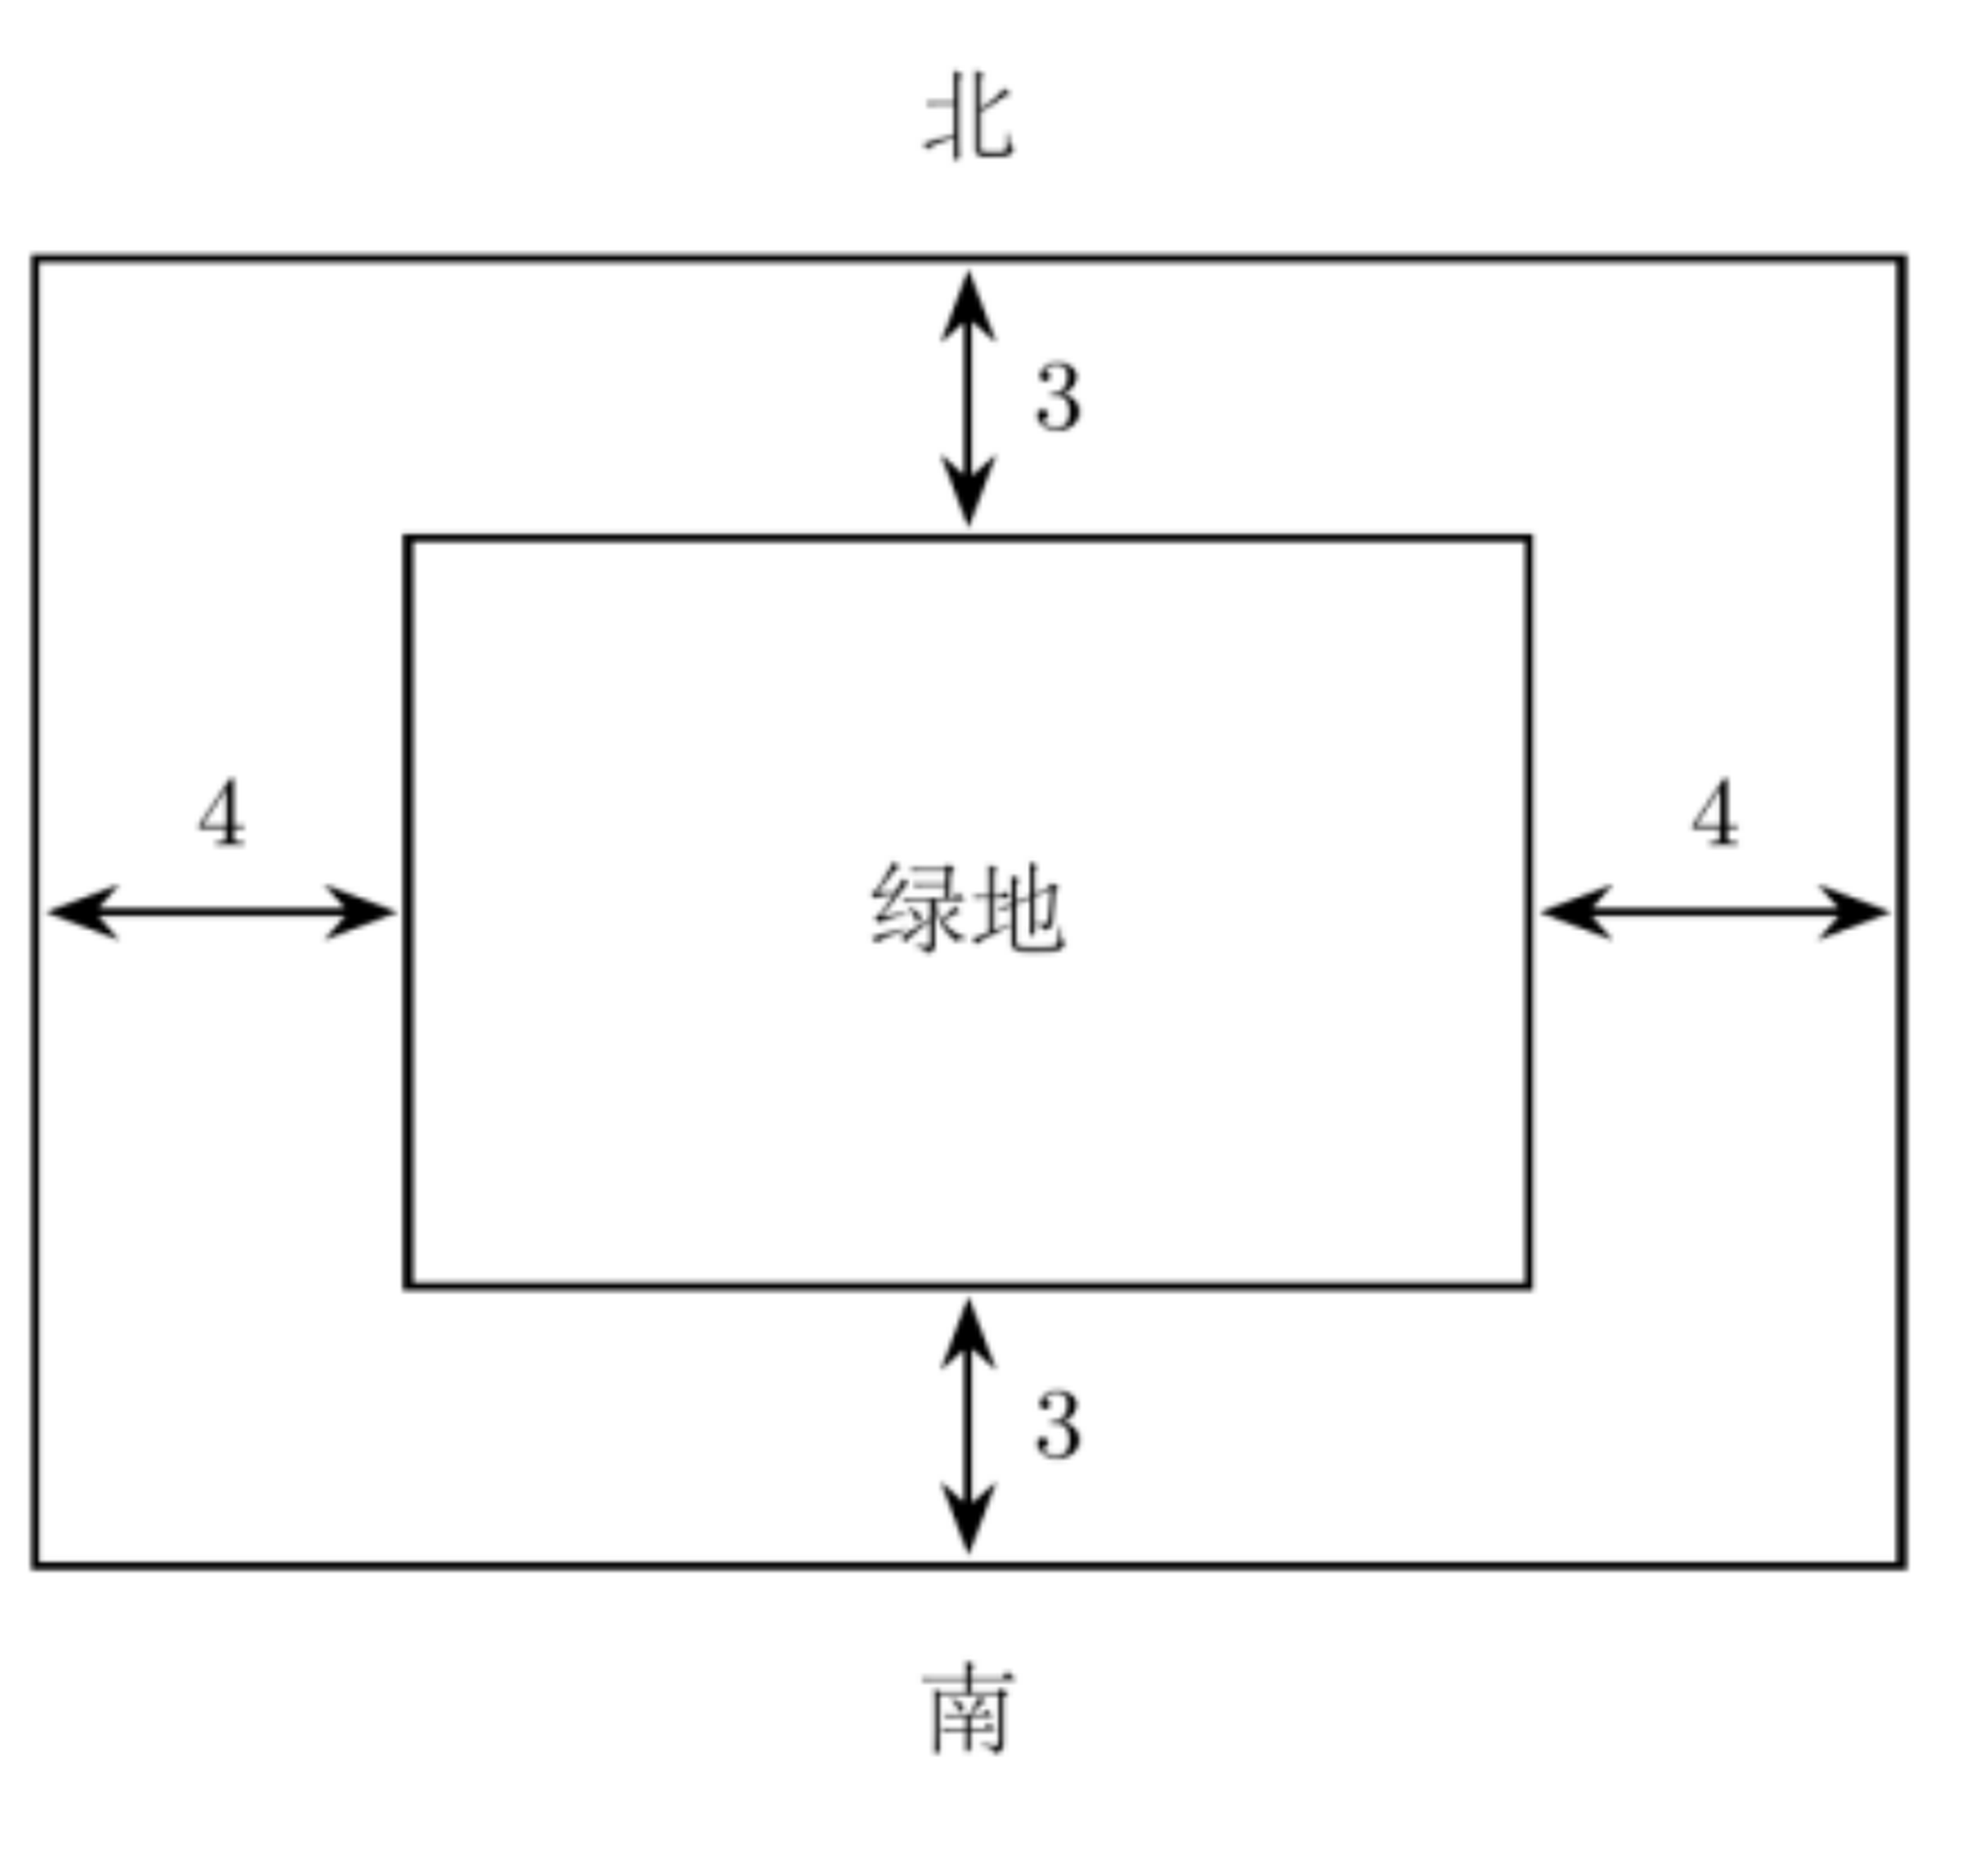
\includegraphics[width=0.32\textwidth]{figures/gao129_q19.png}
\end{center}

(1) 将 $S$ 表示为 $x$ 的函数；

(2) 试确定绿地东西方向的边长和南北方向的边长，使人行道的占地面积最小，并求出人行道的占地最小面积（结果精确到 0.1 米）

\ifanswer
\solbegin
\step{(1) 绿地南北方向的边长为 $\dfrac{1000}{x}$ 米，$x>0$.}
\step{外矩形东西、南北方向的边长分别为 $x+8$ 米、$\dfrac{1000}{x}+6$ 米.}
\step{因此 $S=(x+8)\left(\dfrac{1000}{x}+6\right)-1000=6x+\dfrac{8000}{x}+48, x>0$.}
\step{(2) 因为 $x>0,S=6x+\dfrac{8000}{x}+48\geqslant2\sqrt{6x\cdot\dfrac{8000}{x}}+48=48+80\sqrt{30}$.}
\step{等号当且仅当 $6x=\dfrac{8000}{x}$，即 $x=\dfrac{20\sqrt{30}}{3}\approx36.5$ 时成立，}
\step{此时绿地南北方向的边长为 $\dfrac{1000}{x}=\dfrac{1000}{\dfrac{20\sqrt{30}}{3}}=5\sqrt{30}\approx27.4$（米），}
\step{所以绿地东西方向、南北方向的边长分别约为 36.5 米、27.4 米时，}
\step{人行道的占地面积最小，最小面积为 $S_{min}=48+80\sqrt{30}\approx486.2$ 平方米.}
\solend
\fi

\item 已知集合 $A=\{x\mid x^2-3x+2=0\},B=\{x\mid x^2-ax+a-1=0\}$，

$C=\{x\mid x^2+2(m+1)x+m^2-5=0\}$.

(1) 若 $A=B$，求实数 $a$ 的值；

(2) 若 $B=\{1\}$，求实数 $a$ 的值；

(3) 若 $A\cap C=C$，求实数 $m$ 的取值范围.

\ifanswer
\solbegin
\step{(1) $A=\{1,2\}$，且 $x^2-ax+a-1=(x-1)(x-a+1)$，所以 $B=\{1,a-1\}$，}
\step{因此 $A=B\Leftrightarrow a-1=2\Leftrightarrow a=3$.}
\step{(2) $B=\{1\}$ 表示原方程只有一个不同的实数根，}
\step{得 $a-1=1$，即 $a=2$.}
\step{当 $a=2$ 时，原方程为 $(x-1)^2=0$，符合题意.}
\step{(3) $A\cap C=C\Leftrightarrow C\subseteq\{1,2\}$，}
\step{方程的判别式为 $\Delta=[2(m+1)]^2-4(m^2-5)=8(m+3)$.}
\step{当 $m<-3$ 时，$\Delta<0, C=\varnothing$，满足条件.}
\step{当 $m=-3$ 时，原方程为 $(x-2)^2=0, C=\{2\}$，满足条件.}
\step{当 $m>-3$ 时，方程有两个不同的实数根，必须有 $C=\{1,2\}$，}
\step{由韦达定理，$\begin{cases}-2(m+1)=1+2=3\\m^2-5=1\cdot2=2\end{cases}$，}
\step{第一式得 $m=-\dfrac52$，但此时 $m^2-5=\dfrac54\neq2$，不合题意.}
\step{因此 $m$ 的取值范围为 $(-\infty,-3]$.}
\solend
\fi

\item 设函数 $f(x)=ax^2+(1-a)x+a-2(a\in\R)$.

(1) 若关于 $x$ 的不等式 $f(x)\leqslant0$ 的解集为 $\left[0,\dfrac12\right]$，求实数 $a$ 的值；

(2) 若不等式 $f(x)\geqslant-2$ 对于实数 $a\in[-1,1]$ 时恒成立，求 $x$ 的取值范围；

(3) 解关于 $x$ 的不等式：$f(x)<a-1$.

\ifanswer
\solbegin
\step{(1) 由题意得 $0,\dfrac12$ 是方程 $ax^2+(1-a)x+a-2=0$ 的两个根，}
\step{则 $\begin{cases}0+\dfrac12=-\dfrac{1-a}{a}\\0\times\dfrac12=\dfrac{a-2}{a}\end{cases}\Rightarrow a=2$；}
\step{(2) $ax^2+(1-a)x+a-2\geqslant-2\Rightarrow a(x^2-x+1)+x\geqslant0$ 对 $a\in[-1,1]$ 恒成立，}
\step{则 $\begin{cases}-(x^2-x+1)+x\geqslant0\\(x^2-x+1)+x\geqslant0\end{cases}\Rightarrow\begin{cases}x=1\\x\in\R\end{cases}\Rightarrow x=1$，则 $x$ 的取值范围为 $\{1\}$；}
\step{(3) $f(x)<a-1$ 等价于 $ax^2+(1-a)x-1<0$，}
\step{当 $a=0$ 时，不等式可化为 $x<1$，解集为 $\{x\mid x<1\}$，}
\step{当 $a>0$ 时，不等式可化为 $(ax+1)(x-1)<0$，解集为 $\{x\mid -\dfrac1a<x<1\}$；}
\step{当 $a<0$ 时，不等式化为 $(ax+1)(x-1)<0$，}
\step{①当 $a=-1$ 时，$-\dfrac1a=1$，不等式的解集为 $\{x\mid x\neq1\}$；}
\step{②当 $-1<a<0$ 时，$-\dfrac1a>1$，不等式的解集为 $\{x\mid x<1$ 或 $x>-\dfrac1a\}$；}
\step{③当 $a<-1$ 时，$-\dfrac1a<1$，不等式的解集为 $\{x\mid x<-\dfrac1a$ 或 $x>1\}$；}
\step{综上，当 $a<-1$ 时，解集为 $\{x\mid x<-\dfrac1a$ 或 $x>1\}$；}
\step{当 $a=-1$ 时，解集为 $\{x\mid x\neq1\}$；}
\step{当 $-1<a<0$ 时，解集为 $\{x\mid x<1$ 或 $x>-\dfrac1a\}$；}
\step{当 $a=0$ 时，解集为 $\{x\mid x<1\}$；}
\step{当 $a>0$ 时，解集为 $\{x\mid -\dfrac1a<x<1\}$.}
\solend
\fi

\end{enumerate}

\end{document}
"
%
% 原始材料：微信公众号"魔都数学加油站"文章，作者破晓，2026-11-12 18:56 发布；
% 连载"27学年高一129"，原文标题"27学年高一129——2026-2027年上海市立达中学高一上期中"；
% 原文链接：https://mp.weixin.qq.com/s/gJhGsOBiWi7gW62u8EWLYA。
% 正文为 8 张 PNG 页（01、02、03、05、06 为 4762x6735，04、07、08 为 2560x3620），
% 题目下印有【解析】或【答案】，为讲评版。题目、解析均据原图转录；
% 卷面粉红色水印"魔都数学加油站"及公众号页脚未录入。全卷仅第 19 题有 1 幅插图。
%
% 卷首标题：原卷印作"2026-2027 年立达中学高一上期中"（公众号标题中的"上海市"
% 卷面标题行没有，本稿照卷面），年份区间按全稿惯例排 en dash；原卷未印副标题，
% 本卷为期中卷、跨集合与常用逻辑用语／不等式／函数三章，按题目内容标为
% "集合与常用逻辑用语、不等式、函数"（与 125、126 同为期中卷，口径相同）：
% 集合与逻辑见 Q3、Q4、Q13、Q20，不等式见 Q5、Q6、Q7、Q9、Q10、Q11、Q12、
% Q14、Q15、Q16、Q17、Q18、Q21，函数（含二次函数、基本不等式应用）见 Q8、Q19、Q21。
%
% 与原卷的排版差异：
%   ① 原文从第 3 题起，填空题编号为 3—12、选择题为 13—16、解答题为 17—21，本稿保留原题号；
%   ② 原卷每题下直接印【解析】／【答案】，本稿按全稿惯例置于答案版；第 3、5 题只印
%      【答案】，另提 \ans{}；第 13—16 题答案均在【解析】末句"故选 …"，题干括号内留空、
%      不另提 \ans{}；四道选择题括号内原卷均未印答案；
%   ③ 原卷未印副标题，本稿按"知识模块"口径补出（见上"卷首标题"）；
%   ④ 原卷填空横线按全稿惯例排为 \blankline[4.4em]；选择题括号排 \mbox{（\quad）}、
%      选项段前按惯例加 \keepwithprev；解答题不留作答区（原卷为讲评版，与 109—128 同）；
%   ⑤ 原卷数集排斜体 $R$，按全稿惯例改 \R；绝对值排 \lvert…\rvert，集合描述竖线排 \mid；
%      不等号按全稿惯例排 \leqslant／\geqslant；子题标号原卷一律用半角括号 (1)(2)(3)，本稿照录；
%   ⑥ 原卷第 19 题插图浮排在 Q18 解析右侧、"19."题干之上，本稿按体例就近置于 Q19
%      题干"如图所示"之后（居中 \includegraphics），图取原卷截图去水印；题前按惯例加
%      \needvspace{7cm} 守卫（照 高一120／127 成例），保证"题干 + 图"整块不被页边界切开；
%   ⑦ 原卷 Q8 解析续头印在第 2 页页首、Q17 解析续头印在第 5 页页首、Q19 题干续在第 6 页、
%      Q20 解析跨 6—7 页、Q21 解析续头印在第 8 页页首，本稿按题合并连续排版；
%      末页第 8 页为 Q21 解析的续尾，按实际印刷行单列（照 高一127 第 09 页续尾成例）。
%
% 判别式字形：第 8 题解析 $\Delta=m^2+4m>0$、第 10 题解析 $\Delta=k^2+6k=k(k+6)<0$、
%   第 20 题 (3) 解析 $\Delta=[2(m+1)]^2-4(m^2-5)=8(m+3)$ 三处原卷均排 $\Delta$
%   （等腰、高；回原图逐处放大核对、三处字形一致），照录 \Delta；全卷未出现 \triangle
%   （等边、扁）。
%
% 子集符号：第 13 题 ② $\{0,1,2\}\subseteq\{2,1,0\}$、③ $\varnothing\subseteq\{0,1,2\}$，
%   第 17 题 (2)② $B\subseteq A$、$B\subseteq(3,+\infty)$，第 20 题 (3) $C\subseteq\{1,2\}$
%   均印带下划线，照录 \subseteq；全卷未出现单线 \subset（回原图放大逐处确认）。
%
% 原卷存疑照录：
%   第 15 题解析"即 $m=4$，$n=3$ 时取等号"与题干 $\dfrac1m+n=1$、等号条件
%     $mn=\dfrac9{mn}$ 均不一致（按题应为 $n=\dfrac34$），照录、未统一；
%   第 18 题 (1) 题干"设 $M=2x^2+3x-1,N=7x-3$ 比较 $M$ 与 $N$ 两个数的大小"
%     两式间用半角逗号、且"$N=7x-3$"后无标点直接接"比较"，照录；
%   第 11 题解析"$1-x+2x-1=-(3x-2), 4x=2, x=\dfrac12$"、第 14 题解析
%     "$a=2, b=1, c=4, d=0$"、第 19 题解析"$6x+\dfrac{8000}{x}+48, x>0$"、
%     第 20 题解析"$\Delta<0, C=\varnothing$"与"$(x-2)^2=0, C=\{2\}$"、
%     第 12 题解析"$(x+y)^2=3+t\geqslant0,(x-y)^2=3-3t\geqslant0$"等处数学式内
%     用半角逗号，照录；
%   第 19 题题干"如图所示（图中单位：米）设绿地东西方向的边长为 $x$"在右括号后
%     无标点直接续"设"，照录；
%   第 21 题 (3) 解析先按 $a>0$、$a=0$、$a<0$ 分述解集，又在"综上"处重列全部
%     五类（含已给出的 $a>0$、$a=0$），照录；
%   第 21 题 (2) 题干与解析均作 $f(x)\geqslant-2$（与 $a(x^2-x+1)+x\geqslant0$ 相符），
%     照录，勿误读为 $f(x)\geqslant2$。
%
% 行数复核：逐题数 \step 条数，合计 93 条（Q3：0；Q4：2；Q5：0；Q6：3；Q7：3；
% Q8：2；Q9：4；Q10：3；Q11：5；Q12：5；Q13：1；Q14：3；Q15：3；Q16：7；
% Q17：7；Q18：8；Q19：8；Q20：13；Q21：16），与原卷印刷行逐题相等
% （cases 块作一个印刷行计）。第 3、5 题只印【答案】，提 \ans{}，不计入 \step 账；
% 四道选择题答案均在解析末句，括号内留空、不另提 \ans{}。
%
\documentclass[a4paper,11pt]{article}
\usepackage{common}

\begin{document}

\examtitlest[3]{2026--2027 年立达中学高一上期中}{集合与常用逻辑用语、不等式、函数}

\bigsec{一、填空题}

\begin{enumerate}
\setcounter{enumi}{2}

\item 若 $A=\{x\mid -3<x\leqslant2\},B=\{x\mid 1<x\leqslant3\}$，则 $A\cup B=$\blankline[4.4em].

\ifanswer
\ans{$(-3,3]$}
\fi

\item 若 $A$ 是 $B$ 的必要非充分条件，$B$ 是 $C$ 的充要条件，$C$ 是 $D$ 的必要非充分条件，则 $D$ 是 $A$ 的\blankline[4.4em]条件.

\ifanswer
\solbegin
\step{$D\Rightarrow C\Leftrightarrow B\Rightarrow A$，且 $A\nRightarrow B$，因此 $D\Rightarrow A$ 且 $A\nRightarrow D$，}
\step{故 $D$ 是 $A$ 的充分非必要条件.}
\solend
\fi

\item 不等式 $\dfrac1x<1$ 的解集为\blankline[4.4em].

\ifanswer
\ans{$(-\infty,0)\cup(1,+\infty)$}
\fi

\item 已知正实数 $x$、$y$ 满足 $2x+y=2$，则 $xy$ 的最大值为\blankline[4.4em].

\ifanswer
\solbegin
\step{因为 $x>0$，$y>0$，所以 $2x+y\geqslant2\sqrt{2xy}$（当且仅当 $2x=y$ 时，取等号），}
\step{又因为 $2x+y=2$，所以 $2\geqslant2\sqrt{2xy}$（当且仅当 $2x=y$ 时，取等号），}
\step{即 $xy\leqslant\dfrac12$，则 $xy$ 的最大值为 $\dfrac12$.}
\solend
\fi

\item 已知 $x\in\R$，函数 $y=\lvert x+2\rvert+\lvert x-3\rvert$ 的最小值为\blankline[4.4em].

\ifanswer
\solbegin
\step{由 $\lvert x+2\rvert+\lvert x-3\rvert\geqslant\lvert(x+2)-(x-3)\rvert=5$，}
\step{当且仅当 $(x+2)(x-3)\leqslant0$，即 $-2\leqslant x\leqslant3$ 时，上式取等号，}
\step{则函数 $y=\lvert x+2\rvert+\lvert x-3\rvert$ 的最小值是 5.}
\solend
\fi

\item 已知实系数一元二次方程 $x^2+mx-m=0$ 的两根分别为 $x_1,x_2$，且 $\lvert x_1-x_2\rvert=\sqrt{21}$，实数 $m$ 的值为\blankline[4.4em].

\ifanswer
\solbegin
\step{由题意得 $\Delta=m^2+4m>0$，解得 $m>0$ 或 $m<-4,x_1+x_2=-m,x_1x_2=-m$，}
\step{则 $\lvert x_1-x_2\rvert=\sqrt{(x_1+x_2)^2-4x_1x_2}=\sqrt{m^2+4m}=\sqrt{21}$，解得 $m=-7$ 或 $3$.}
\solend
\fi

\item 已知不等式 $ax^2-5x+b>0$ 的解集是 $\{x\mid -3<x<-2\}$，则不等式 $bx^2-5x+a>0$ 的解集是\blankline[4.4em].

\ifanswer
\solbegin
\step{$ax^2-5x+b=a(x+3)(x+2)$，比较系数得 $5a=-5,b=6a$，}
\step{即 $a=-1,b=-6$.}
\step{$bx^2-5x+a>0\Leftrightarrow(3x+1)(2x+1)<0\Leftrightarrow-\dfrac12<x<-\dfrac13$，}
\step{故解集为 $\left\{x\mid -\dfrac12<x<-\dfrac13\right\}$.}
\solend
\fi

\item 不等式 $4kx^2+kx-\dfrac38<0$ 对于一切实数 $x$ 都成立，则实数 $k$ 的取值范围是\blankline[4.4em].

\ifanswer
\solbegin
\step{$k=0$ 时，不等式恒成立；}
\step{$k\neq0$ 时，须 $4k<0$ 且 $\Delta=k^2+6k=k(k+6)<0$，解得 $-6<k<0$.}
\step{因此 $k\in(-6,0]$.}
\solend
\fi

\item 设 $x\in\R$，方程 $\lvert 1-x\rvert+\lvert 2x-1\rvert=\lvert 3x-2\rvert$ 的解集为\blankline[4.4em].

\ifanswer
\solbegin
\step{当 $x\leqslant\dfrac12$ 时，方程化为 $1-x-(2x-1)=-(3x-2)$，$2-3x=-3x+2$，恒成立，}
\step{当 $\dfrac12<x\leqslant\dfrac23$ 时，方程化为 $1-x+2x-1=-(3x-2), 4x=2, x=\dfrac12$，不合题意，}
\step{当 $\dfrac23<x\leqslant1$ 时，方程化为 $1-x+2x-1=3x-2$，$2x=2$，解得 $x=1$，}
\step{当 $x>1$ 时，方程化为 $-(1-x)+2x-1=3x-2$，$3x-2=3x-2$，恒成立，}
\step{综上所述，$\lvert 1-x\rvert+\lvert 2x-1\rvert=\lvert 3x-2\rvert$ 的解集为 $\left(-\infty,\dfrac12\right]\cup[1,+\infty)$.}
\solend
\fi

\item 已知非零实数 $x,y$ 满足 $x^2+xy+y^2=3$，则 $x^2-xy+y^2$ 的取值范围是\blankline[4.4em].

\ifanswer
\solbegin
\step{令 $t=xy\neq0$，由 $(x+y)^2=3+t\geqslant0,(x-y)^2=3-3t\geqslant0$，}
\step{得 $t\in[-3,0)\cup(0,1]$.}
\step{对上述任意 $t$，联立 $x+y=\sqrt{3+t},x-y=\sqrt{3-3t}$，所得 $x,y$ 满足原条件，}
\step{因此上述 $t$ 均可取到.}
\step{于是 $x^2-xy+y^2=3-2t$ 的取值范围为 $[1,3)\cup(3,9]$.}
\solend
\fi

\end{enumerate}

\bigsec{二、选择题}

\begin{enumerate}
\setcounter{enumi}{12}

\item 下列各式中，正确的个数是\mbox{（\quad）}

① $\{0\}\in\{0,1,2\}$；② $\{0,1,2\}\subseteq\{2,1,0\}$；③ $\varnothing\subseteq\{0,1,2\}$；④ $\varnothing=\{0\}$；⑤ $\{0,1\}=\{(0,1)\}$；

⑥ $0=\{0\}$.

\keepwithprev
A. $1$\qquad\qquad B. $2$\qquad\qquad C. $3$\qquad\qquad D. $4$

\ifanswer
\solbegin
\step{①不正确，②正确，③正确，④不正确，⑤不正确，⑥不正确. 故选 $B$.}
\solend
\fi

\item 下列四个命题中，为真命题的是\mbox{（\quad）}

\keepwithprev
A. 若 $a>b$，则 $ac^2>bc^2$\qquad\qquad B. 若 $a>b,c>d$，则 $a-c>b-d$

C. 若 $ac^2>bc^2$，则 $a>b$\qquad\qquad D. 若 $a>b$，则 $\dfrac1a<\dfrac1b$

\ifanswer
\solbegin
\step{C 中，$(a-b)c^2>0$，必有 $c^2>0$ 且 $a-b>0$，即 $a>b$.}
\step{A 取 $c=0$；B 取 $a=2, b=1, c=4, d=0$；D 取 $a=1, b=-1$，均不成立.}
\step{故选 $C$.}
\solend
\fi

\item 已知 $m$、$n\in(0,+\infty)$，$\dfrac1m+n=1$，则 $m+\dfrac9n$ 的最小值为\mbox{（\quad）}

\keepwithprev
A. $13$\qquad\qquad B. $16$\qquad\qquad C. $3$\qquad\qquad D. $6$

\ifanswer
\solbegin
\step{因为 $m$、$n\in(0,+\infty)$，$\dfrac1m+n=1$，}
\step{所以 $m+\dfrac9n=(m+\dfrac9n)(\dfrac1m+n)=10+mn+\dfrac9{mn}\geqslant10+2\sqrt{mn\cdot\dfrac9{mn}}=16$，}
\step{当且仅当 $mn=\dfrac9{mn}$，即 $m=4$，$n=3$ 时取等号. 故选 $B$.}
\solend
\fi

\item 下列不等式：① $\left\lvert x+\dfrac1x\right\rvert\geqslant2$；② $x^2+2x+1>0$；③ $\lvert x\rvert+\lvert x-1\rvert\geqslant1$；④ $\dfrac{x}{x^2+x+1}<1$；

解集为 $\R$ 的不等式的个数是\mbox{（\quad）}

\keepwithprev
A. $0$\qquad\qquad B. $1$\qquad\qquad C. $2$\qquad\qquad D. $3$

\ifanswer
\solbegin
\step{对于①，当 $x=0$ 时，$\dfrac1x$ 无意义，故 $\left\lvert x+\dfrac1x\right\rvert\geqslant2$ 的解集不是 $\R$，错误；}
\step{对于②，$x^2+2x+1=(x+1)^2\geqslant0$，当 $x=-1$ 取到等号，解集不是 $\R$，故错误；}
\step{对于③，$\lvert x\rvert+\lvert x-1\rvert\geqslant\lvert x-(x-1)\rvert=1$，当 $x(x-1)\leqslant0$ 时取等号，解集为 $\R$，}
\step{故正确；}
\step{对于④，由于 $x^2+x+1>0$ 恒成立，}
\step{故 $\dfrac{x}{x^2+x+1}<1$ 等价于 $x<x^2+x+1\Rightarrow x^2+1>0$ 恒成立，故解集为 $\R$，正确，}
\step{故正确的有③④，故选 $C$.}
\solend
\fi

\end{enumerate}

\bigsec{三、解答题}

\begin{enumerate}
\setcounter{enumi}{16}

\item (1) 解不等式组 $\begin{cases}\dfrac{x+3}{x+1}\leqslant2\\\lvert 2x-3\rvert\leqslant2\end{cases}$.

(2) 已知集合 $A=\{x\mid -x+3<0\},B=\{x\mid a\leqslant x\leqslant a+3\}$.

①当 $a=2$，求集合 $A\cap B$；

②若 $A\cup B=A$，求实数 $a$ 的取值范围.

\ifanswer
\solbegin
\step{(1) 由 $\begin{cases}\dfrac{x+3}{x+1}\leqslant2\\\lvert 2x-3\rvert\leqslant2\end{cases}$ 得 $\begin{cases}\dfrac{x+3-2x-2}{x+1}\leqslant0\\-2\leqslant2x-3\leqslant2\end{cases}$，即 $\begin{cases}\dfrac{-x+1}{x+1}\leqslant0\\1\leqslant2x\leqslant5\end{cases}$，则 $\begin{cases}\dfrac{x-1}{x+1}\geqslant0\\\dfrac12\leqslant x\leqslant\dfrac52\end{cases}$，}
\step{解得 $1\leqslant x\leqslant\dfrac52$，即原不等式组的解集为 $\left[1,\dfrac52\right]$.}
\step{(2) $-x+3<0\Leftrightarrow x>3$，所以 $A=(3,+\infty)$.}
\step{①当 $a=2$ 时，$B=[2,5], A\cap B=(3,+\infty)\cap[2,5]=(3,5]$.}
\step{②$A\cup B=A\Leftrightarrow B\subseteq A$.}
\step{因为 $B=[a,a+3]$，且左端点 $a\in B$，所以 $B\subseteq(3,+\infty)\Leftrightarrow a>3$，}
\step{实数 $a$ 的取值范围为 $(3,+\infty)$.}
\solend
\fi

\item (1) 设 $M=2x^2+3x-1,N=7x-3$ 比较 $M$ 与 $N$ 两个数的大小.

(2) 解关于 $x$ 的不等式：$x^2-(a+3)x+3a<0$，$a\in\R$.

\ifanswer
\solbegin
\step{(1) $M-N=2x^2+3x-1-(7x-3)=2(x-1)^2$.}
\step{$x=1$ 时，$M-N=0$，即 $M=N$.}
\step{$x\neq1$ 时，$M-N>0$，即 $M>N$.}
\step{(2) 不等式 $x^2-(a+3)x+3a<0$ 可化为 $(x-3)(x-a)<0$，}
\step{不等式对应方程的解为 $a$ 和 3，}
\step{当 $a<3$ 时，不等式 $x^2-(a+3)x+3a<0$ 的解集为 $(a,3)$，}
\step{当 $a=3$ 时，不等式 $x^2-(a+3)x+3a<0$ 的解集为 $\varnothing$，}
\step{当 $a>3$ 时，不等式 $x^2-(a+3)x+3a<0$ 的解集为 $(3,a)$.}
\solend
\fi

% 第 19 题是"题干 + 图"约 7cm 的一整块，答案版实测断点落在题干之后（图被推到次页页首），
% 照 高一120／127 成例在题前先量一次页高，不够就把"题干 + 图"整块一起挪到次页。
\needvspace{7cm}
\item 某新建居民小区欲建一面积为 1000 平方米的矩形绿地，在绿地四周铺设人行道，设计要求绿地南北两侧人行道宽 3 米，东西两侧人行道宽 4 米，如图所示（图中单位：米）设绿地东西方向的边长为 $x$，人行道的占地面积为 $S$.

\begin{center}
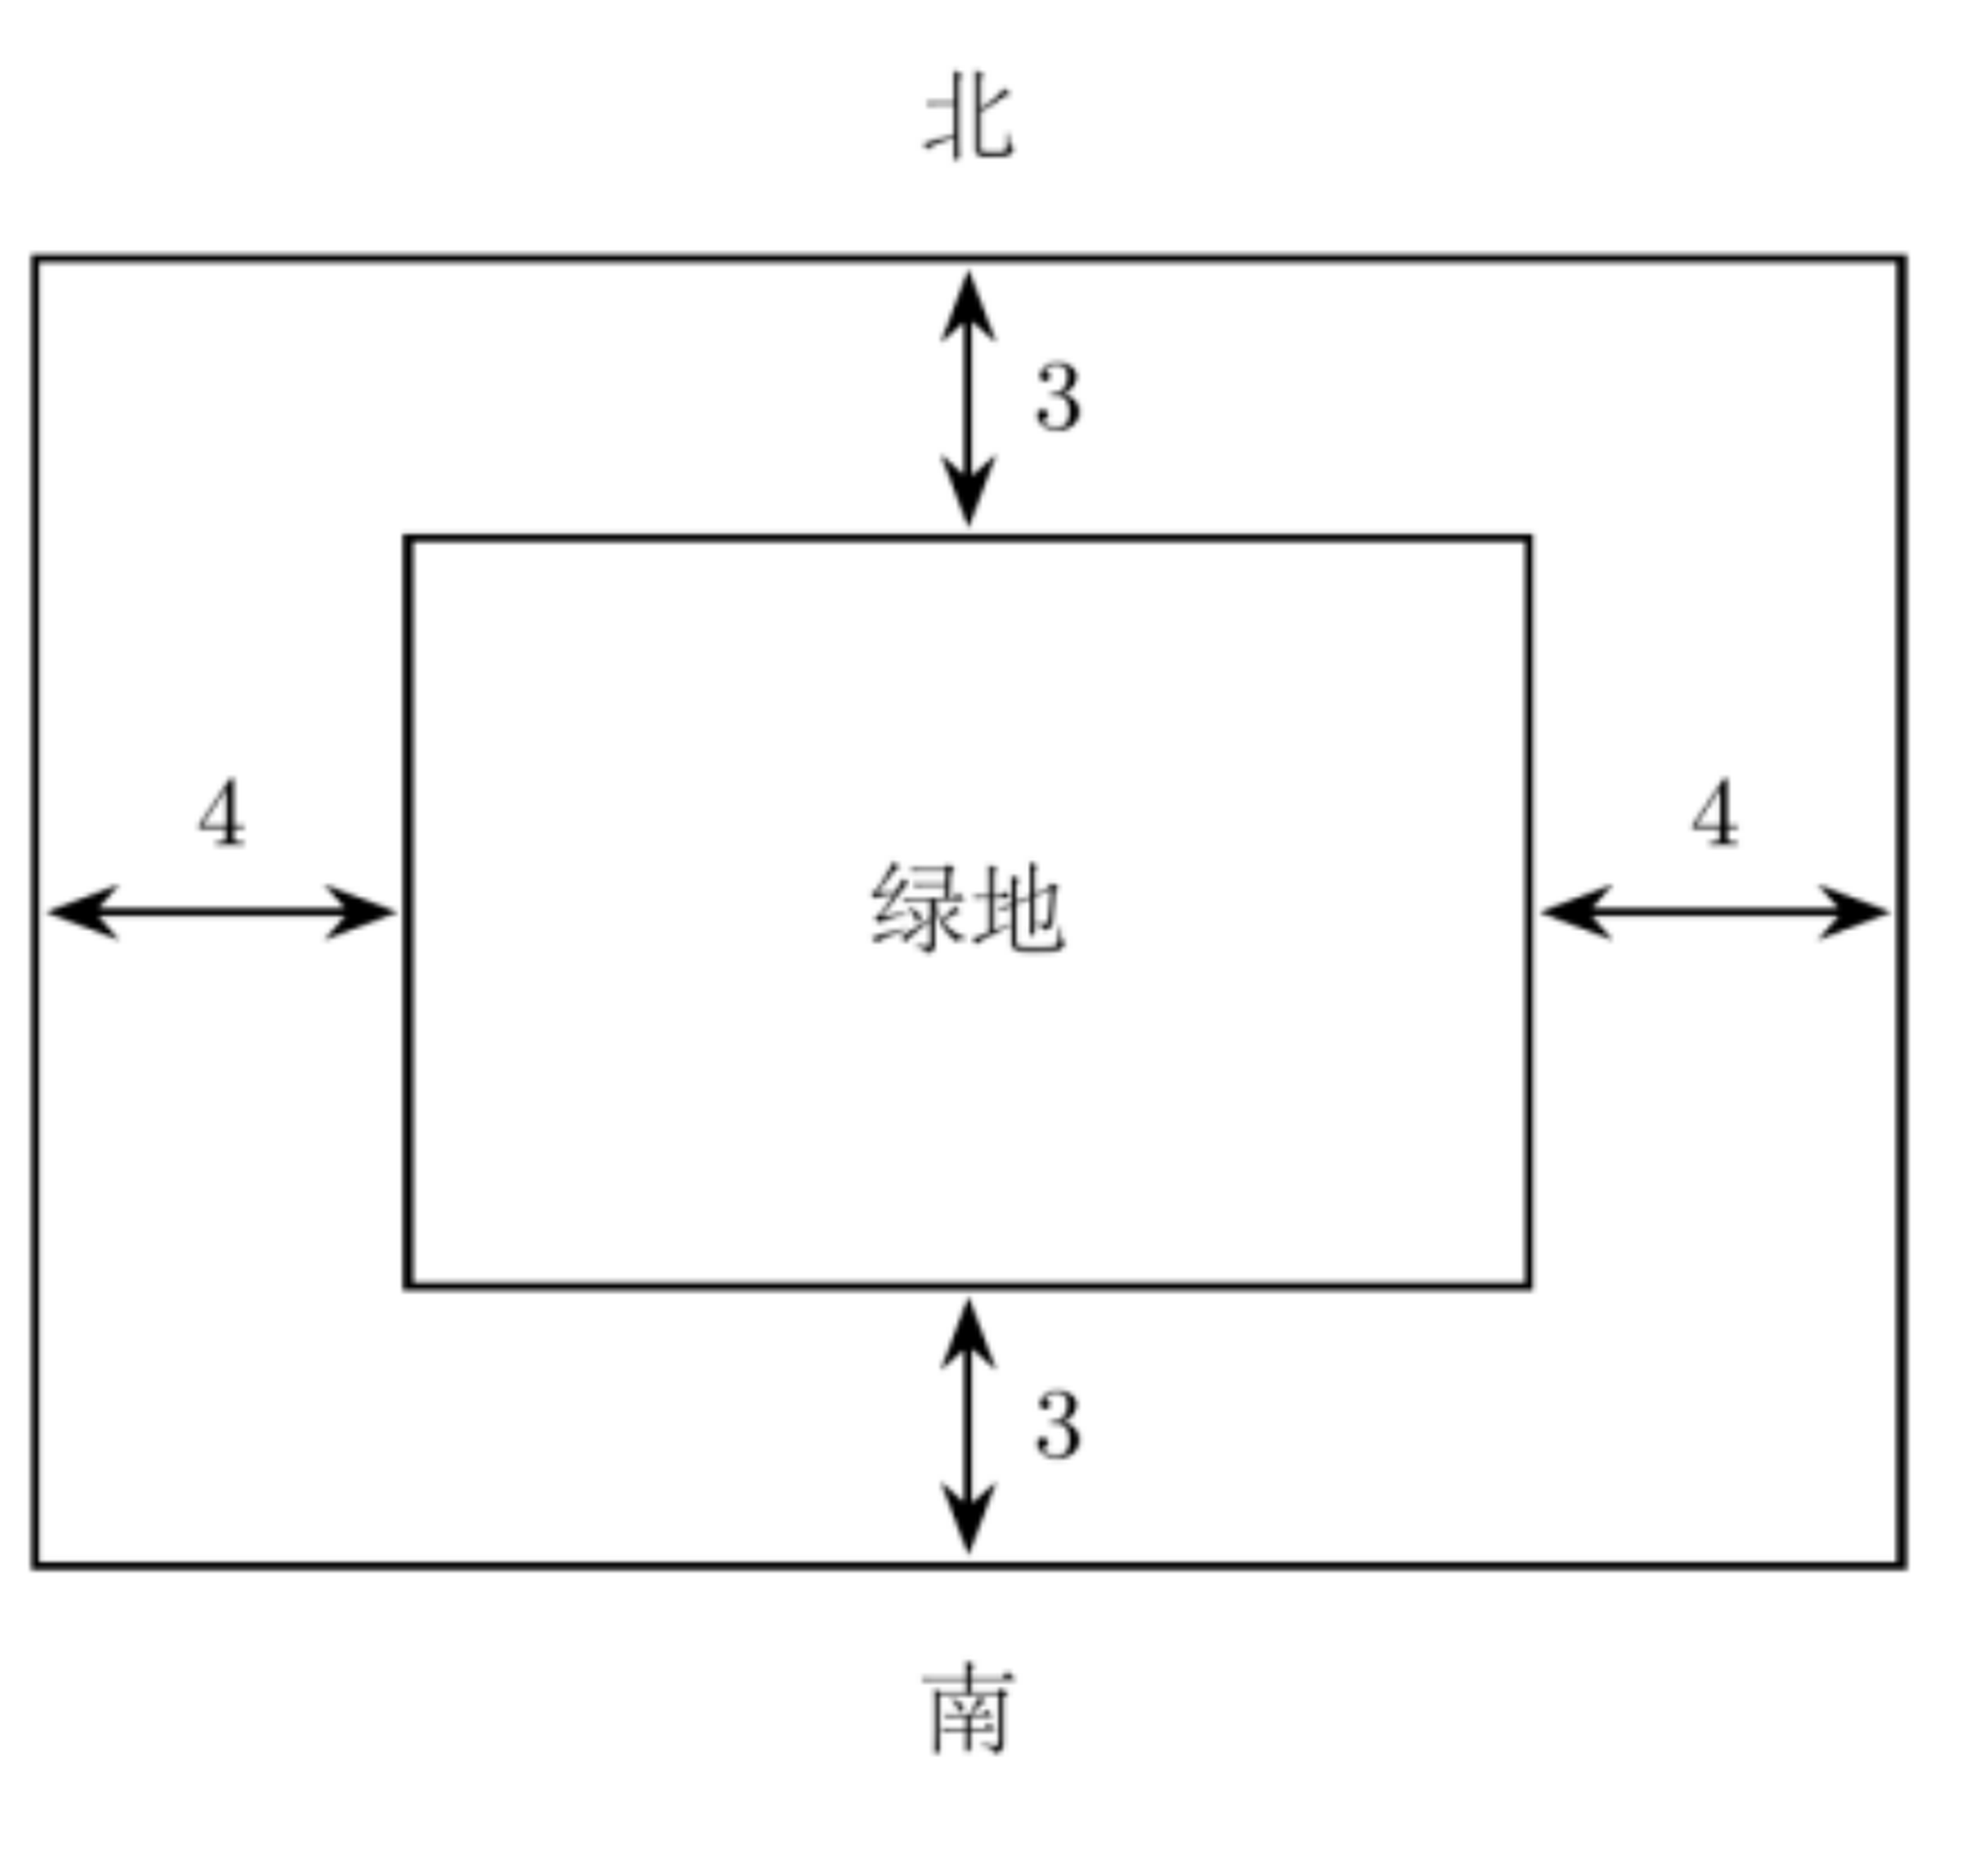
\includegraphics[width=0.32\textwidth]{figures/gao129_q19.png}
\end{center}

(1) 将 $S$ 表示为 $x$ 的函数；

(2) 试确定绿地东西方向的边长和南北方向的边长，使人行道的占地面积最小，并求出人行道的占地最小面积（结果精确到 0.1 米）

\ifanswer
\solbegin
\step{(1) 绿地南北方向的边长为 $\dfrac{1000}{x}$ 米，$x>0$.}
\step{外矩形东西、南北方向的边长分别为 $x+8$ 米、$\dfrac{1000}{x}+6$ 米.}
\step{因此 $S=(x+8)\left(\dfrac{1000}{x}+6\right)-1000=6x+\dfrac{8000}{x}+48, x>0$.}
\step{(2) 因为 $x>0,S=6x+\dfrac{8000}{x}+48\geqslant2\sqrt{6x\cdot\dfrac{8000}{x}}+48=48+80\sqrt{30}$.}
\step{等号当且仅当 $6x=\dfrac{8000}{x}$，即 $x=\dfrac{20\sqrt{30}}{3}\approx36.5$ 时成立，}
\step{此时绿地南北方向的边长为 $\dfrac{1000}{x}=\dfrac{1000}{\dfrac{20\sqrt{30}}{3}}=5\sqrt{30}\approx27.4$（米），}
\step{所以绿地东西方向、南北方向的边长分别约为 36.5 米、27.4 米时，}
\step{人行道的占地面积最小，最小面积为 $S_{min}=48+80\sqrt{30}\approx486.2$ 平方米.}
\solend
\fi

\item 已知集合 $A=\{x\mid x^2-3x+2=0\},B=\{x\mid x^2-ax+a-1=0\}$，

$C=\{x\mid x^2+2(m+1)x+m^2-5=0\}$.

(1) 若 $A=B$，求实数 $a$ 的值；

(2) 若 $B=\{1\}$，求实数 $a$ 的值；

(3) 若 $A\cap C=C$，求实数 $m$ 的取值范围.

\ifanswer
\solbegin
\step{(1) $A=\{1,2\}$，且 $x^2-ax+a-1=(x-1)(x-a+1)$，所以 $B=\{1,a-1\}$，}
\step{因此 $A=B\Leftrightarrow a-1=2\Leftrightarrow a=3$.}
\step{(2) $B=\{1\}$ 表示原方程只有一个不同的实数根，}
\step{得 $a-1=1$，即 $a=2$.}
\step{当 $a=2$ 时，原方程为 $(x-1)^2=0$，符合题意.}
\step{(3) $A\cap C=C\Leftrightarrow C\subseteq\{1,2\}$，}
\step{方程的判别式为 $\Delta=[2(m+1)]^2-4(m^2-5)=8(m+3)$.}
\step{当 $m<-3$ 时，$\Delta<0, C=\varnothing$，满足条件.}
\step{当 $m=-3$ 时，原方程为 $(x-2)^2=0, C=\{2\}$，满足条件.}
\step{当 $m>-3$ 时，方程有两个不同的实数根，必须有 $C=\{1,2\}$，}
\step{由韦达定理，$\begin{cases}-2(m+1)=1+2=3\\m^2-5=1\cdot2=2\end{cases}$，}
\step{第一式得 $m=-\dfrac52$，但此时 $m^2-5=\dfrac54\neq2$，不合题意.}
\step{因此 $m$ 的取值范围为 $(-\infty,-3]$.}
\solend
\fi

\item 设函数 $f(x)=ax^2+(1-a)x+a-2(a\in\R)$.

(1) 若关于 $x$ 的不等式 $f(x)\leqslant0$ 的解集为 $\left[0,\dfrac12\right]$，求实数 $a$ 的值；

(2) 若不等式 $f(x)\geqslant-2$ 对于实数 $a\in[-1,1]$ 时恒成立，求 $x$ 的取值范围；

(3) 解关于 $x$ 的不等式：$f(x)<a-1$.

\ifanswer
\solbegin
\step{(1) 由题意得 $0,\dfrac12$ 是方程 $ax^2+(1-a)x+a-2=0$ 的两个根，}
\step{则 $\begin{cases}0+\dfrac12=-\dfrac{1-a}{a}\\0\times\dfrac12=\dfrac{a-2}{a}\end{cases}\Rightarrow a=2$；}
\step{(2) $ax^2+(1-a)x+a-2\geqslant-2\Rightarrow a(x^2-x+1)+x\geqslant0$ 对 $a\in[-1,1]$ 恒成立，}
\step{则 $\begin{cases}-(x^2-x+1)+x\geqslant0\\(x^2-x+1)+x\geqslant0\end{cases}\Rightarrow\begin{cases}x=1\\x\in\R\end{cases}\Rightarrow x=1$，则 $x$ 的取值范围为 $\{1\}$；}
\step{(3) $f(x)<a-1$ 等价于 $ax^2+(1-a)x-1<0$，}
\step{当 $a=0$ 时，不等式可化为 $x<1$，解集为 $\{x\mid x<1\}$，}
\step{当 $a>0$ 时，不等式可化为 $(ax+1)(x-1)<0$，解集为 $\{x\mid -\dfrac1a<x<1\}$；}
\step{当 $a<0$ 时，不等式化为 $(ax+1)(x-1)<0$，}
\step{①当 $a=-1$ 时，$-\dfrac1a=1$，不等式的解集为 $\{x\mid x\neq1\}$；}
\step{②当 $-1<a<0$ 时，$-\dfrac1a>1$，不等式的解集为 $\{x\mid x<1$ 或 $x>-\dfrac1a\}$；}
\step{③当 $a<-1$ 时，$-\dfrac1a<1$，不等式的解集为 $\{x\mid x<-\dfrac1a$ 或 $x>1\}$；}
\step{综上，当 $a<-1$ 时，解集为 $\{x\mid x<-\dfrac1a$ 或 $x>1\}$；}
\step{当 $a=-1$ 时，解集为 $\{x\mid x\neq1\}$；}
\step{当 $-1<a<0$ 时，解集为 $\{x\mid x<1$ 或 $x>-\dfrac1a\}$；}
\step{当 $a=0$ 时，解集为 $\{x\mid x<1\}$；}
\step{当 $a>0$ 时，解集为 $\{x\mid -\dfrac1a<x<1\}$.}
\solend
\fi

\end{enumerate}

\end{document}
"
%
% 原始材料：微信公众号"魔都数学加油站"文章，作者破晓，2026-11-12 18:56 发布；
% 连载"27学年高一129"，原文标题"27学年高一129——2026-2027年上海市立达中学高一上期中"；
% 原文链接：https://mp.weixin.qq.com/s/gJhGsOBiWi7gW62u8EWLYA。
% 正文为 8 张 PNG 页（01、02、03、05、06 为 4762x6735，04、07、08 为 2560x3620），
% 题目下印有【解析】或【答案】，为讲评版。题目、解析均据原图转录；
% 卷面粉红色水印"魔都数学加油站"及公众号页脚未录入。全卷仅第 19 题有 1 幅插图。
%
% 卷首标题：原卷印作"2026-2027 年立达中学高一上期中"（公众号标题中的"上海市"
% 卷面标题行没有，本稿照卷面），年份区间按全稿惯例排 en dash；原卷未印副标题，
% 本卷为期中卷、跨集合与常用逻辑用语／不等式／函数三章，按题目内容标为
% "集合与常用逻辑用语、不等式、函数"（与 125、126 同为期中卷，口径相同）：
% 集合与逻辑见 Q3、Q4、Q13、Q20，不等式见 Q5、Q6、Q7、Q9、Q10、Q11、Q12、
% Q14、Q15、Q16、Q17、Q18、Q21，函数（含二次函数、基本不等式应用）见 Q8、Q19、Q21。
%
% 与原卷的排版差异：
%   ① 原文从第 3 题起，填空题编号为 3—12、选择题为 13—16、解答题为 17—21，本稿保留原题号；
%   ② 原卷每题下直接印【解析】／【答案】，本稿按全稿惯例置于答案版；第 3、5 题只印
%      【答案】，另提 \ans{}；第 13—16 题答案均在【解析】末句"故选 …"，题干括号内留空、
%      不另提 \ans{}；四道选择题括号内原卷均未印答案；
%   ③ 原卷未印副标题，本稿按"知识模块"口径补出（见上"卷首标题"）；
%   ④ 原卷填空横线按全稿惯例排为 \blankline[4.4em]；选择题括号排 \mbox{（\quad）}、
%      选项段前按惯例加 \keepwithprev；解答题不留作答区（原卷为讲评版，与 109—128 同）；
%   ⑤ 原卷数集排斜体 $R$，按全稿惯例改 \R；绝对值排 \lvert…\rvert，集合描述竖线排 \mid；
%      不等号按全稿惯例排 \leqslant／\geqslant；子题标号原卷一律用半角括号 (1)(2)(3)，本稿照录；
%   ⑥ 原卷第 19 题插图浮排在 Q18 解析右侧、"19."题干之上，本稿按体例就近置于 Q19
%      题干"如图所示"之后（居中 \includegraphics），图取原卷截图去水印；题前按惯例加
%      \needvspace{7cm} 守卫（照 高一120／127 成例），保证"题干 + 图"整块不被页边界切开；
%   ⑦ 原卷 Q8 解析续头印在第 2 页页首、Q17 解析续头印在第 5 页页首、Q19 题干续在第 6 页、
%      Q20 解析跨 6—7 页、Q21 解析续头印在第 8 页页首，本稿按题合并连续排版；
%      末页第 8 页为 Q21 解析的续尾，按实际印刷行单列（照 高一127 第 09 页续尾成例）。
%
% 判别式字形：第 8 题解析 $\Delta=m^2+4m>0$、第 10 题解析 $\Delta=k^2+6k=k(k+6)<0$、
%   第 20 题 (3) 解析 $\Delta=[2(m+1)]^2-4(m^2-5)=8(m+3)$ 三处原卷均排 $\Delta$
%   （等腰、高；回原图逐处放大核对、三处字形一致），照录 \Delta；全卷未出现 \triangle
%   （等边、扁）。
%
% 子集符号：第 13 题 ② $\{0,1,2\}\subseteq\{2,1,0\}$、③ $\varnothing\subseteq\{0,1,2\}$，
%   第 17 题 (2)② $B\subseteq A$、$B\subseteq(3,+\infty)$，第 20 题 (3) $C\subseteq\{1,2\}$
%   均印带下划线，照录 \subseteq；全卷未出现单线 \subset（回原图放大逐处确认）。
%
% 原卷存疑照录：
%   第 15 题解析"即 $m=4$，$n=3$ 时取等号"与题干 $\dfrac1m+n=1$、等号条件
%     $mn=\dfrac9{mn}$ 均不一致（按题应为 $n=\dfrac34$），照录、未统一；
%   第 18 题 (1) 题干"设 $M=2x^2+3x-1,N=7x-3$ 比较 $M$ 与 $N$ 两个数的大小"
%     两式间用半角逗号、且"$N=7x-3$"后无标点直接接"比较"，照录；
%   第 11 题解析"$1-x+2x-1=-(3x-2), 4x=2, x=\dfrac12$"、第 14 题解析
%     "$a=2, b=1, c=4, d=0$"、第 19 题解析"$6x+\dfrac{8000}{x}+48, x>0$"、
%     第 20 题解析"$\Delta<0, C=\varnothing$"与"$(x-2)^2=0, C=\{2\}$"、
%     第 12 题解析"$(x+y)^2=3+t\geqslant0,(x-y)^2=3-3t\geqslant0$"等处数学式内
%     用半角逗号，照录；
%   第 19 题题干"如图所示（图中单位：米）设绿地东西方向的边长为 $x$"在右括号后
%     无标点直接续"设"，照录；
%   第 21 题 (3) 解析先按 $a>0$、$a=0$、$a<0$ 分述解集，又在"综上"处重列全部
%     五类（含已给出的 $a>0$、$a=0$），照录；
%   第 21 题 (2) 题干与解析均作 $f(x)\geqslant-2$（与 $a(x^2-x+1)+x\geqslant0$ 相符），
%     照录，勿误读为 $f(x)\geqslant2$。
%
% 行数复核：逐题数 \step 条数，合计 93 条（Q3：0；Q4：2；Q5：0；Q6：3；Q7：3；
% Q8：2；Q9：4；Q10：3；Q11：5；Q12：5；Q13：1；Q14：3；Q15：3；Q16：7；
% Q17：7；Q18：8；Q19：8；Q20：13；Q21：16），与原卷印刷行逐题相等
% （cases 块作一个印刷行计）。第 3、5 题只印【答案】，提 \ans{}，不计入 \step 账；
% 四道选择题答案均在解析末句，括号内留空、不另提 \ans{}。
%
\documentclass[a4paper,11pt]{article}
\usepackage{common}

\begin{document}

\examtitlest[3]{2026--2027 年立达中学高一上期中}{集合与常用逻辑用语、不等式、函数}

\bigsec{一、填空题}

\begin{enumerate}
\setcounter{enumi}{2}

\item 若 $A=\{x\mid -3<x\leqslant2\},B=\{x\mid 1<x\leqslant3\}$，则 $A\cup B=$\blankline[4.4em].

\ifanswer
\ans{$(-3,3]$}
\fi

\item 若 $A$ 是 $B$ 的必要非充分条件，$B$ 是 $C$ 的充要条件，$C$ 是 $D$ 的必要非充分条件，则 $D$ 是 $A$ 的\blankline[4.4em]条件.

\ifanswer
\solbegin
\step{$D\Rightarrow C\Leftrightarrow B\Rightarrow A$，且 $A\nRightarrow B$，因此 $D\Rightarrow A$ 且 $A\nRightarrow D$，}
\step{故 $D$ 是 $A$ 的充分非必要条件.}
\solend
\fi

\item 不等式 $\dfrac1x<1$ 的解集为\blankline[4.4em].

\ifanswer
\ans{$(-\infty,0)\cup(1,+\infty)$}
\fi

\item 已知正实数 $x$、$y$ 满足 $2x+y=2$，则 $xy$ 的最大值为\blankline[4.4em].

\ifanswer
\solbegin
\step{因为 $x>0$，$y>0$，所以 $2x+y\geqslant2\sqrt{2xy}$（当且仅当 $2x=y$ 时，取等号），}
\step{又因为 $2x+y=2$，所以 $2\geqslant2\sqrt{2xy}$（当且仅当 $2x=y$ 时，取等号），}
\step{即 $xy\leqslant\dfrac12$，则 $xy$ 的最大值为 $\dfrac12$.}
\solend
\fi

\item 已知 $x\in\R$，函数 $y=\lvert x+2\rvert+\lvert x-3\rvert$ 的最小值为\blankline[4.4em].

\ifanswer
\solbegin
\step{由 $\lvert x+2\rvert+\lvert x-3\rvert\geqslant\lvert(x+2)-(x-3)\rvert=5$，}
\step{当且仅当 $(x+2)(x-3)\leqslant0$，即 $-2\leqslant x\leqslant3$ 时，上式取等号，}
\step{则函数 $y=\lvert x+2\rvert+\lvert x-3\rvert$ 的最小值是 5.}
\solend
\fi

\item 已知实系数一元二次方程 $x^2+mx-m=0$ 的两根分别为 $x_1,x_2$，且 $\lvert x_1-x_2\rvert=\sqrt{21}$，实数 $m$ 的值为\blankline[4.4em].

\ifanswer
\solbegin
\step{由题意得 $\Delta=m^2+4m>0$，解得 $m>0$ 或 $m<-4,x_1+x_2=-m,x_1x_2=-m$，}
\step{则 $\lvert x_1-x_2\rvert=\sqrt{(x_1+x_2)^2-4x_1x_2}=\sqrt{m^2+4m}=\sqrt{21}$，解得 $m=-7$ 或 $3$.}
\solend
\fi

\item 已知不等式 $ax^2-5x+b>0$ 的解集是 $\{x\mid -3<x<-2\}$，则不等式 $bx^2-5x+a>0$ 的解集是\blankline[4.4em].

\ifanswer
\solbegin
\step{$ax^2-5x+b=a(x+3)(x+2)$，比较系数得 $5a=-5,b=6a$，}
\step{即 $a=-1,b=-6$.}
\step{$bx^2-5x+a>0\Leftrightarrow(3x+1)(2x+1)<0\Leftrightarrow-\dfrac12<x<-\dfrac13$，}
\step{故解集为 $\left\{x\mid -\dfrac12<x<-\dfrac13\right\}$.}
\solend
\fi

\item 不等式 $4kx^2+kx-\dfrac38<0$ 对于一切实数 $x$ 都成立，则实数 $k$ 的取值范围是\blankline[4.4em].

\ifanswer
\solbegin
\step{$k=0$ 时，不等式恒成立；}
\step{$k\neq0$ 时，须 $4k<0$ 且 $\Delta=k^2+6k=k(k+6)<0$，解得 $-6<k<0$.}
\step{因此 $k\in(-6,0]$.}
\solend
\fi

\item 设 $x\in\R$，方程 $\lvert 1-x\rvert+\lvert 2x-1\rvert=\lvert 3x-2\rvert$ 的解集为\blankline[4.4em].

\ifanswer
\solbegin
\step{当 $x\leqslant\dfrac12$ 时，方程化为 $1-x-(2x-1)=-(3x-2)$，$2-3x=-3x+2$，恒成立，}
\step{当 $\dfrac12<x\leqslant\dfrac23$ 时，方程化为 $1-x+2x-1=-(3x-2), 4x=2, x=\dfrac12$，不合题意，}
\step{当 $\dfrac23<x\leqslant1$ 时，方程化为 $1-x+2x-1=3x-2$，$2x=2$，解得 $x=1$，}
\step{当 $x>1$ 时，方程化为 $-(1-x)+2x-1=3x-2$，$3x-2=3x-2$，恒成立，}
\step{综上所述，$\lvert 1-x\rvert+\lvert 2x-1\rvert=\lvert 3x-2\rvert$ 的解集为 $\left(-\infty,\dfrac12\right]\cup[1,+\infty)$.}
\solend
\fi

\item 已知非零实数 $x,y$ 满足 $x^2+xy+y^2=3$，则 $x^2-xy+y^2$ 的取值范围是\blankline[4.4em].

\ifanswer
\solbegin
\step{令 $t=xy\neq0$，由 $(x+y)^2=3+t\geqslant0,(x-y)^2=3-3t\geqslant0$，}
\step{得 $t\in[-3,0)\cup(0,1]$.}
\step{对上述任意 $t$，联立 $x+y=\sqrt{3+t},x-y=\sqrt{3-3t}$，所得 $x,y$ 满足原条件，}
\step{因此上述 $t$ 均可取到.}
\step{于是 $x^2-xy+y^2=3-2t$ 的取值范围为 $[1,3)\cup(3,9]$.}
\solend
\fi

\end{enumerate}

\bigsec{二、选择题}

\begin{enumerate}
\setcounter{enumi}{12}

\item 下列各式中，正确的个数是\mbox{（\quad）}

① $\{0\}\in\{0,1,2\}$；② $\{0,1,2\}\subseteq\{2,1,0\}$；③ $\varnothing\subseteq\{0,1,2\}$；④ $\varnothing=\{0\}$；⑤ $\{0,1\}=\{(0,1)\}$；

⑥ $0=\{0\}$.

\keepwithprev
A. $1$\qquad\qquad B. $2$\qquad\qquad C. $3$\qquad\qquad D. $4$

\ifanswer
\solbegin
\step{①不正确，②正确，③正确，④不正确，⑤不正确，⑥不正确. 故选 $B$.}
\solend
\fi

\item 下列四个命题中，为真命题的是\mbox{（\quad）}

\keepwithprev
A. 若 $a>b$，则 $ac^2>bc^2$\qquad\qquad B. 若 $a>b,c>d$，则 $a-c>b-d$

C. 若 $ac^2>bc^2$，则 $a>b$\qquad\qquad D. 若 $a>b$，则 $\dfrac1a<\dfrac1b$

\ifanswer
\solbegin
\step{C 中，$(a-b)c^2>0$，必有 $c^2>0$ 且 $a-b>0$，即 $a>b$.}
\step{A 取 $c=0$；B 取 $a=2, b=1, c=4, d=0$；D 取 $a=1, b=-1$，均不成立.}
\step{故选 $C$.}
\solend
\fi

\item 已知 $m$、$n\in(0,+\infty)$，$\dfrac1m+n=1$，则 $m+\dfrac9n$ 的最小值为\mbox{（\quad）}

\keepwithprev
A. $13$\qquad\qquad B. $16$\qquad\qquad C. $3$\qquad\qquad D. $6$

\ifanswer
\solbegin
\step{因为 $m$、$n\in(0,+\infty)$，$\dfrac1m+n=1$，}
\step{所以 $m+\dfrac9n=(m+\dfrac9n)(\dfrac1m+n)=10+mn+\dfrac9{mn}\geqslant10+2\sqrt{mn\cdot\dfrac9{mn}}=16$，}
\step{当且仅当 $mn=\dfrac9{mn}$，即 $m=4$，$n=3$ 时取等号. 故选 $B$.}
\solend
\fi

\item 下列不等式：① $\left\lvert x+\dfrac1x\right\rvert\geqslant2$；② $x^2+2x+1>0$；③ $\lvert x\rvert+\lvert x-1\rvert\geqslant1$；④ $\dfrac{x}{x^2+x+1}<1$；

解集为 $\R$ 的不等式的个数是\mbox{（\quad）}

\keepwithprev
A. $0$\qquad\qquad B. $1$\qquad\qquad C. $2$\qquad\qquad D. $3$

\ifanswer
\solbegin
\step{对于①，当 $x=0$ 时，$\dfrac1x$ 无意义，故 $\left\lvert x+\dfrac1x\right\rvert\geqslant2$ 的解集不是 $\R$，错误；}
\step{对于②，$x^2+2x+1=(x+1)^2\geqslant0$，当 $x=-1$ 取到等号，解集不是 $\R$，故错误；}
\step{对于③，$\lvert x\rvert+\lvert x-1\rvert\geqslant\lvert x-(x-1)\rvert=1$，当 $x(x-1)\leqslant0$ 时取等号，解集为 $\R$，}
\step{故正确；}
\step{对于④，由于 $x^2+x+1>0$ 恒成立，}
\step{故 $\dfrac{x}{x^2+x+1}<1$ 等价于 $x<x^2+x+1\Rightarrow x^2+1>0$ 恒成立，故解集为 $\R$，正确，}
\step{故正确的有③④，故选 $C$.}
\solend
\fi

\end{enumerate}

\bigsec{三、解答题}

\begin{enumerate}
\setcounter{enumi}{16}

\item (1) 解不等式组 $\begin{cases}\dfrac{x+3}{x+1}\leqslant2\\\lvert 2x-3\rvert\leqslant2\end{cases}$.

(2) 已知集合 $A=\{x\mid -x+3<0\},B=\{x\mid a\leqslant x\leqslant a+3\}$.

①当 $a=2$，求集合 $A\cap B$；

②若 $A\cup B=A$，求实数 $a$ 的取值范围.

\ifanswer
\solbegin
\step{(1) 由 $\begin{cases}\dfrac{x+3}{x+1}\leqslant2\\\lvert 2x-3\rvert\leqslant2\end{cases}$ 得 $\begin{cases}\dfrac{x+3-2x-2}{x+1}\leqslant0\\-2\leqslant2x-3\leqslant2\end{cases}$，即 $\begin{cases}\dfrac{-x+1}{x+1}\leqslant0\\1\leqslant2x\leqslant5\end{cases}$，则 $\begin{cases}\dfrac{x-1}{x+1}\geqslant0\\\dfrac12\leqslant x\leqslant\dfrac52\end{cases}$，}
\step{解得 $1\leqslant x\leqslant\dfrac52$，即原不等式组的解集为 $\left[1,\dfrac52\right]$.}
\step{(2) $-x+3<0\Leftrightarrow x>3$，所以 $A=(3,+\infty)$.}
\step{①当 $a=2$ 时，$B=[2,5], A\cap B=(3,+\infty)\cap[2,5]=(3,5]$.}
\step{②$A\cup B=A\Leftrightarrow B\subseteq A$.}
\step{因为 $B=[a,a+3]$，且左端点 $a\in B$，所以 $B\subseteq(3,+\infty)\Leftrightarrow a>3$，}
\step{实数 $a$ 的取值范围为 $(3,+\infty)$.}
\solend
\fi

\item (1) 设 $M=2x^2+3x-1,N=7x-3$ 比较 $M$ 与 $N$ 两个数的大小.

(2) 解关于 $x$ 的不等式：$x^2-(a+3)x+3a<0$，$a\in\R$.

\ifanswer
\solbegin
\step{(1) $M-N=2x^2+3x-1-(7x-3)=2(x-1)^2$.}
\step{$x=1$ 时，$M-N=0$，即 $M=N$.}
\step{$x\neq1$ 时，$M-N>0$，即 $M>N$.}
\step{(2) 不等式 $x^2-(a+3)x+3a<0$ 可化为 $(x-3)(x-a)<0$，}
\step{不等式对应方程的解为 $a$ 和 3，}
\step{当 $a<3$ 时，不等式 $x^2-(a+3)x+3a<0$ 的解集为 $(a,3)$，}
\step{当 $a=3$ 时，不等式 $x^2-(a+3)x+3a<0$ 的解集为 $\varnothing$，}
\step{当 $a>3$ 时，不等式 $x^2-(a+3)x+3a<0$ 的解集为 $(3,a)$.}
\solend
\fi

% 第 19 题是"题干 + 图"约 7cm 的一整块，答案版实测断点落在题干之后（图被推到次页页首），
% 照 高一120／127 成例在题前先量一次页高，不够就把"题干 + 图"整块一起挪到次页。
\needvspace{7cm}
\item 某新建居民小区欲建一面积为 1000 平方米的矩形绿地，在绿地四周铺设人行道，设计要求绿地南北两侧人行道宽 3 米，东西两侧人行道宽 4 米，如图所示（图中单位：米）设绿地东西方向的边长为 $x$，人行道的占地面积为 $S$.

\begin{center}
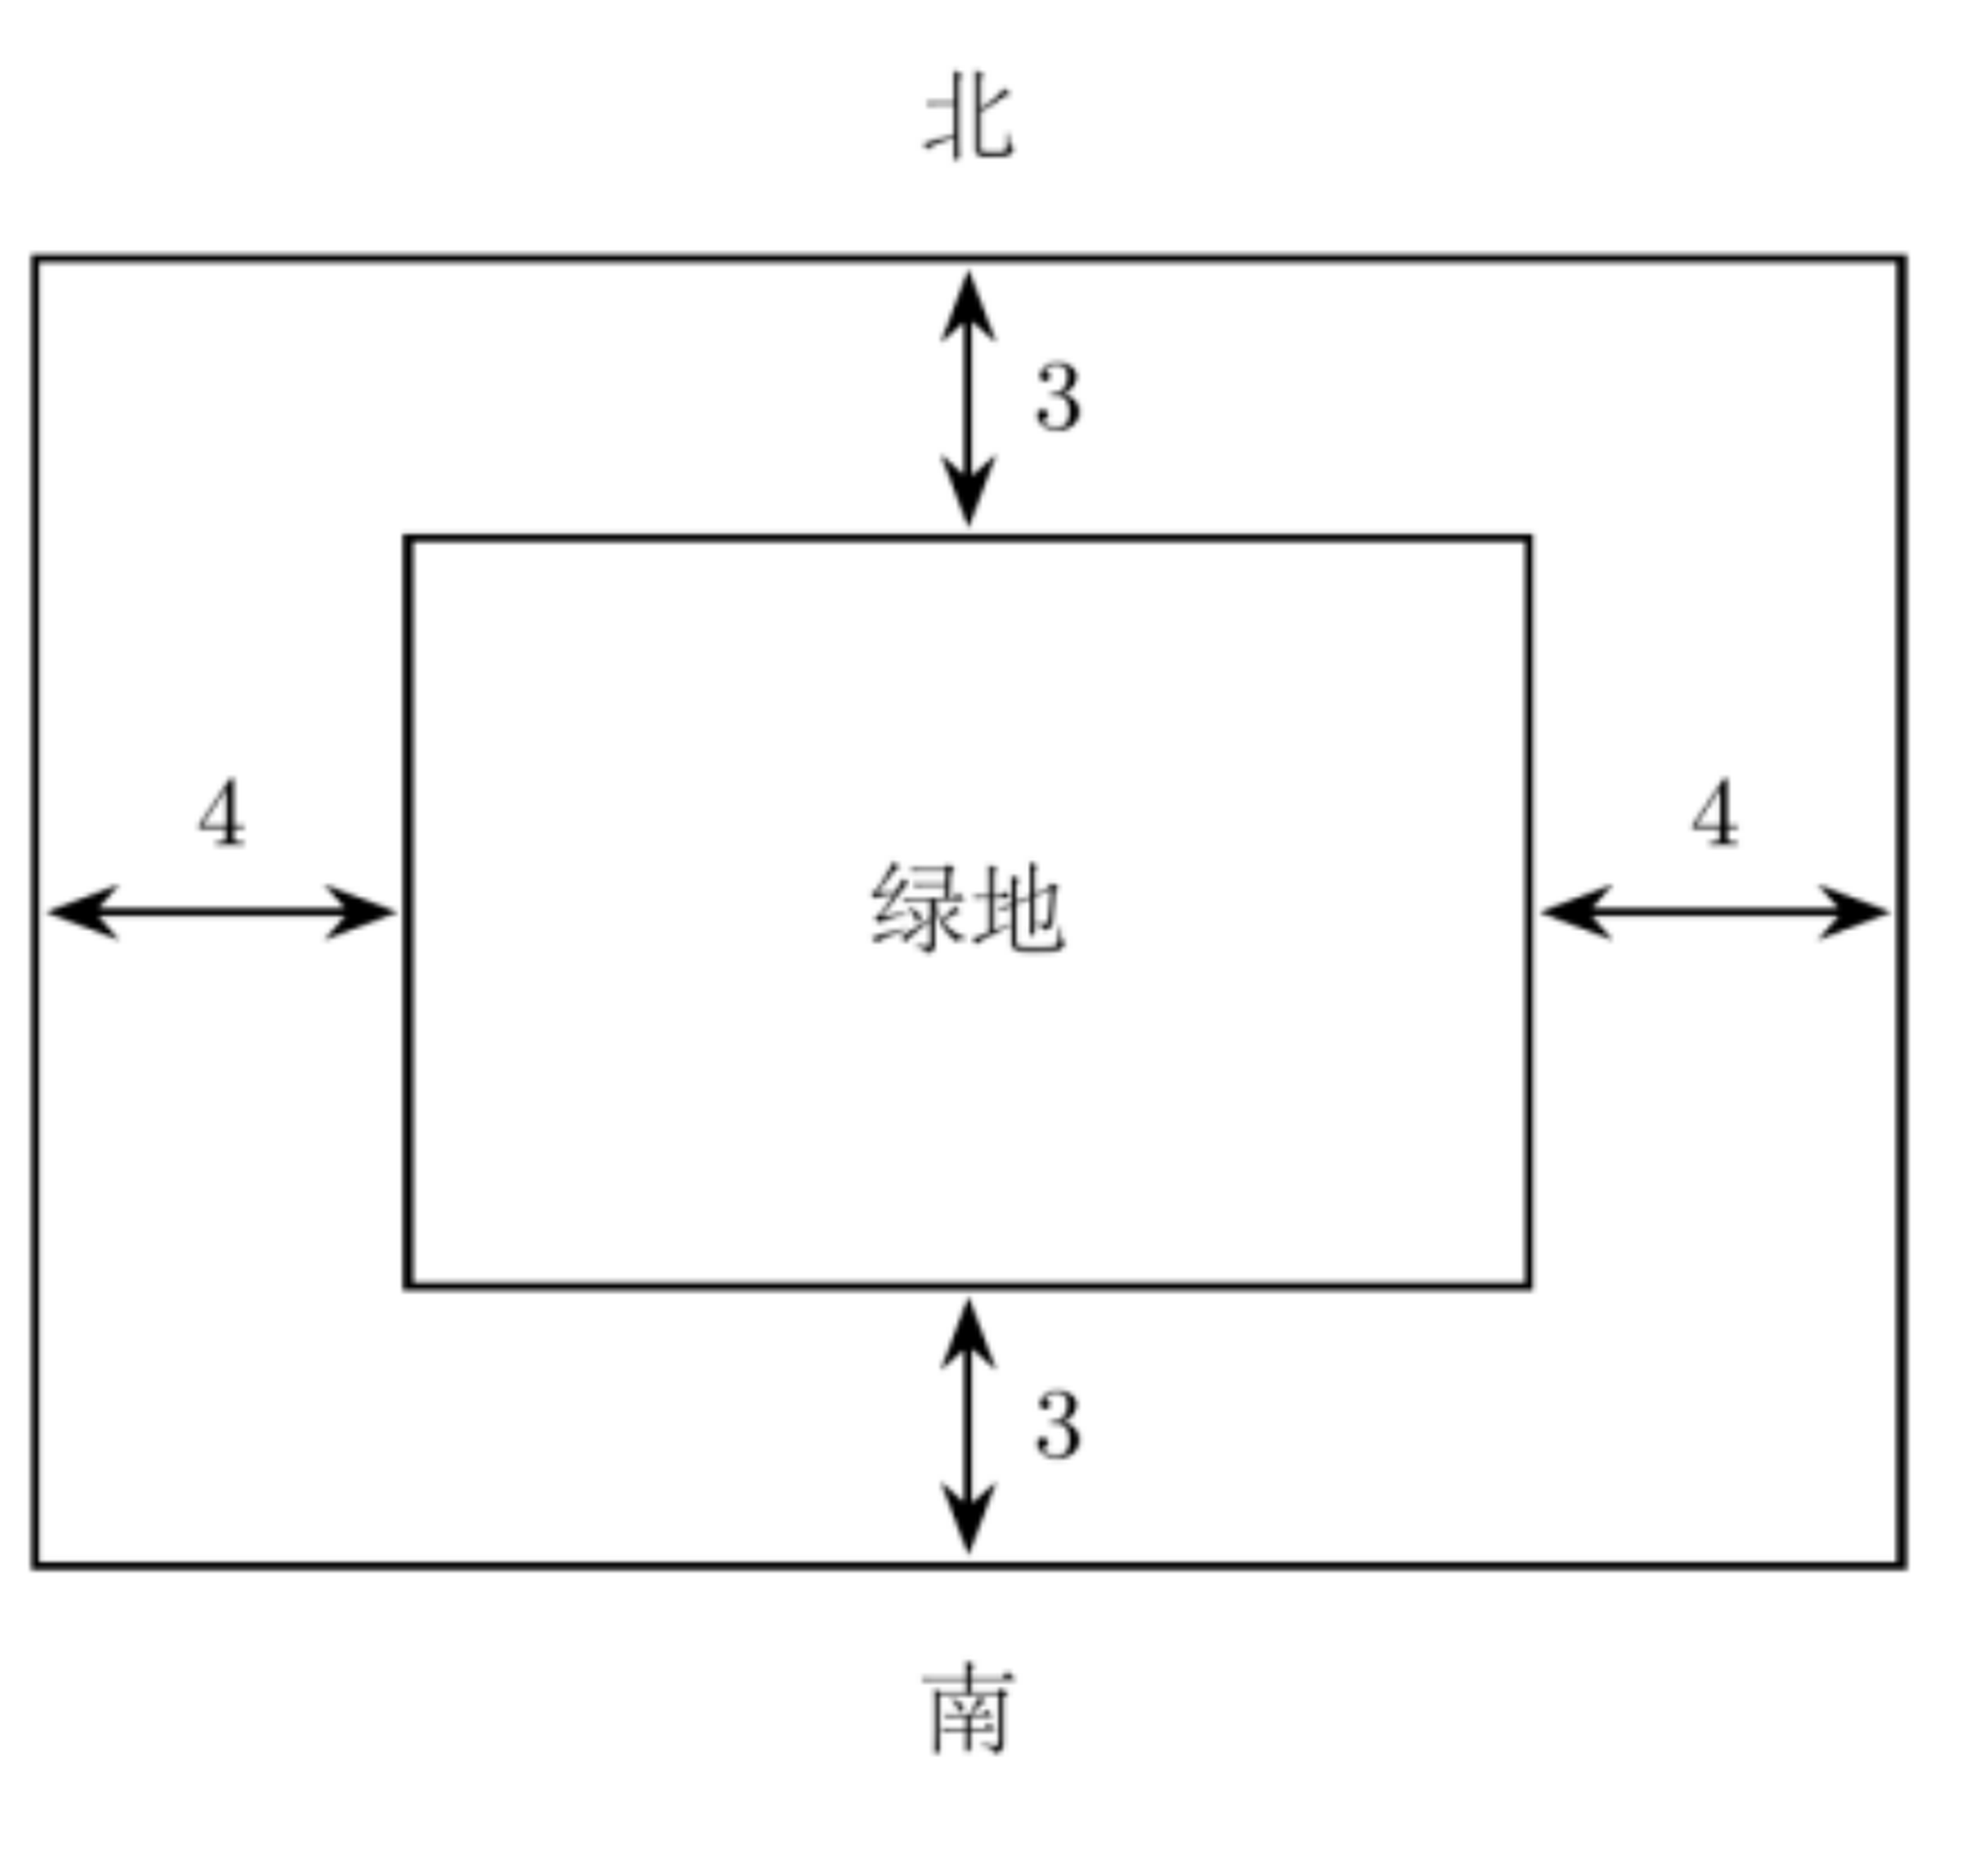
\includegraphics[width=0.32\textwidth]{figures/gao129_q19.png}
\end{center}

(1) 将 $S$ 表示为 $x$ 的函数；

(2) 试确定绿地东西方向的边长和南北方向的边长，使人行道的占地面积最小，并求出人行道的占地最小面积（结果精确到 0.1 米）

\ifanswer
\solbegin
\step{(1) 绿地南北方向的边长为 $\dfrac{1000}{x}$ 米，$x>0$.}
\step{外矩形东西、南北方向的边长分别为 $x+8$ 米、$\dfrac{1000}{x}+6$ 米.}
\step{因此 $S=(x+8)\left(\dfrac{1000}{x}+6\right)-1000=6x+\dfrac{8000}{x}+48, x>0$.}
\step{(2) 因为 $x>0,S=6x+\dfrac{8000}{x}+48\geqslant2\sqrt{6x\cdot\dfrac{8000}{x}}+48=48+80\sqrt{30}$.}
\step{等号当且仅当 $6x=\dfrac{8000}{x}$，即 $x=\dfrac{20\sqrt{30}}{3}\approx36.5$ 时成立，}
\step{此时绿地南北方向的边长为 $\dfrac{1000}{x}=\dfrac{1000}{\dfrac{20\sqrt{30}}{3}}=5\sqrt{30}\approx27.4$（米），}
\step{所以绿地东西方向、南北方向的边长分别约为 36.5 米、27.4 米时，}
\step{人行道的占地面积最小，最小面积为 $S_{min}=48+80\sqrt{30}\approx486.2$ 平方米.}
\solend
\fi

\item 已知集合 $A=\{x\mid x^2-3x+2=0\},B=\{x\mid x^2-ax+a-1=0\}$，

$C=\{x\mid x^2+2(m+1)x+m^2-5=0\}$.

(1) 若 $A=B$，求实数 $a$ 的值；

(2) 若 $B=\{1\}$，求实数 $a$ 的值；

(3) 若 $A\cap C=C$，求实数 $m$ 的取值范围.

\ifanswer
\solbegin
\step{(1) $A=\{1,2\}$，且 $x^2-ax+a-1=(x-1)(x-a+1)$，所以 $B=\{1,a-1\}$，}
\step{因此 $A=B\Leftrightarrow a-1=2\Leftrightarrow a=3$.}
\step{(2) $B=\{1\}$ 表示原方程只有一个不同的实数根，}
\step{得 $a-1=1$，即 $a=2$.}
\step{当 $a=2$ 时，原方程为 $(x-1)^2=0$，符合题意.}
\step{(3) $A\cap C=C\Leftrightarrow C\subseteq\{1,2\}$，}
\step{方程的判别式为 $\Delta=[2(m+1)]^2-4(m^2-5)=8(m+3)$.}
\step{当 $m<-3$ 时，$\Delta<0, C=\varnothing$，满足条件.}
\step{当 $m=-3$ 时，原方程为 $(x-2)^2=0, C=\{2\}$，满足条件.}
\step{当 $m>-3$ 时，方程有两个不同的实数根，必须有 $C=\{1,2\}$，}
\step{由韦达定理，$\begin{cases}-2(m+1)=1+2=3\\m^2-5=1\cdot2=2\end{cases}$，}
\step{第一式得 $m=-\dfrac52$，但此时 $m^2-5=\dfrac54\neq2$，不合题意.}
\step{因此 $m$ 的取值范围为 $(-\infty,-3]$.}
\solend
\fi

\item 设函数 $f(x)=ax^2+(1-a)x+a-2(a\in\R)$.

(1) 若关于 $x$ 的不等式 $f(x)\leqslant0$ 的解集为 $\left[0,\dfrac12\right]$，求实数 $a$ 的值；

(2) 若不等式 $f(x)\geqslant-2$ 对于实数 $a\in[-1,1]$ 时恒成立，求 $x$ 的取值范围；

(3) 解关于 $x$ 的不等式：$f(x)<a-1$.

\ifanswer
\solbegin
\step{(1) 由题意得 $0,\dfrac12$ 是方程 $ax^2+(1-a)x+a-2=0$ 的两个根，}
\step{则 $\begin{cases}0+\dfrac12=-\dfrac{1-a}{a}\\0\times\dfrac12=\dfrac{a-2}{a}\end{cases}\Rightarrow a=2$；}
\step{(2) $ax^2+(1-a)x+a-2\geqslant-2\Rightarrow a(x^2-x+1)+x\geqslant0$ 对 $a\in[-1,1]$ 恒成立，}
\step{则 $\begin{cases}-(x^2-x+1)+x\geqslant0\\(x^2-x+1)+x\geqslant0\end{cases}\Rightarrow\begin{cases}x=1\\x\in\R\end{cases}\Rightarrow x=1$，则 $x$ 的取值范围为 $\{1\}$；}
\step{(3) $f(x)<a-1$ 等价于 $ax^2+(1-a)x-1<0$，}
\step{当 $a=0$ 时，不等式可化为 $x<1$，解集为 $\{x\mid x<1\}$，}
\step{当 $a>0$ 时，不等式可化为 $(ax+1)(x-1)<0$，解集为 $\{x\mid -\dfrac1a<x<1\}$；}
\step{当 $a<0$ 时，不等式化为 $(ax+1)(x-1)<0$，}
\step{①当 $a=-1$ 时，$-\dfrac1a=1$，不等式的解集为 $\{x\mid x\neq1\}$；}
\step{②当 $-1<a<0$ 时，$-\dfrac1a>1$，不等式的解集为 $\{x\mid x<1$ 或 $x>-\dfrac1a\}$；}
\step{③当 $a<-1$ 时，$-\dfrac1a<1$，不等式的解集为 $\{x\mid x<-\dfrac1a$ 或 $x>1\}$；}
\step{综上，当 $a<-1$ 时，解集为 $\{x\mid x<-\dfrac1a$ 或 $x>1\}$；}
\step{当 $a=-1$ 时，解集为 $\{x\mid x\neq1\}$；}
\step{当 $-1<a<0$ 时，解集为 $\{x\mid x<1$ 或 $x>-\dfrac1a\}$；}
\step{当 $a=0$ 时，解集为 $\{x\mid x<1\}$；}
\step{当 $a>0$ 时，解集为 $\{x\mid -\dfrac1a<x<1\}$.}
\solend
\fi

\end{enumerate}

\end{document}
